\documentclass[11pt,a4paper,titlepage]{book}
\usepackage[pdftex]{graphicx}
\usepackage{minitoc}
\usepackage[nottoc]{tocbibind}
\usepackage{fancyheadings}
\usepackage{pdfsync}
\usepackage[latin1]{inputenc}
\usepackage{lettrine}
\usepackage{indentfirst}
\usepackage{alltt}

\usepackage[square,comma]{natbib}
\usepackage[french,english]{babel}
\selectlanguage{english}    % FM, 10.5.2009
% \usepackage{graphicx}
% \usepackage{graphics,ulem,rotating}


% \def\mtctitle{{\sf\bfseries Contents}}  % On change la police pour le titre ``Sommaire''
% \def\stctitle{{\sf\bfseries Contents}}  %
% \def\mtcSfont{\small\sf\bfseries}       % Font des sections : sans serif
\DeclareMathAlphabet{\mathpzc}{OT1}{pzc}{m}{it}

%\usepackage{calc}
%\usepackage{setspace}
%\onehalfspacing
% \usepackage{dimensions} %gère les marges mais c'est pas top!!
 \usepackage[intlimits]{amsmath}
 \usepackage{amsfonts,upgreek,bbm,mathrsfs}
 \usepackage{amssymb,alltt}
 \usepackage{latexsym}  

\usepackage[latin1]{inputenc} 
%\usepackage[sectionbib]{chapterbib}
\usepackage{abbrevjournaux}
% Pour des liens hypertextes + navigation dans le pdf
%\usepackage[backref, pagebackref=true, hyperindex=true, breaklinks=true, colorlinks=true, urlcolor=blue, linkcolor=black, citecolor=blue, citebordercolor=010, pagecolor=red, bookmarks=true, bookmarksopen=true, plainpages=false, pdfpagemode=UseThumbs]{hyperref}

%\usepackage[dvips]{color}
\usepackage{color}
% \usepackage{./astron}

\usepackage{longtable,multirow,enumerate,threeparttable}
 \usepackage{lineno,ulem,cancel}
\usepackage{theorem,algorithm,algorithmic}
\usepackage[ruled,vlined,algochapter,algo2e]{algorithm2e}
\def\newblock{\hskip .11em plus .33em minus .07em}

\bibpunct{(}{)}{;}{a}{}{,}


\bibliographystyle{astron}
% \bibliographystyle{plainnat}

\usepackage{theorem}
\usepackage{chemarrow}
 \usepackage{amsfonts,upgreek,bbm,mathrsfs}
\usepackage{setspace,ulem}
\usepackage{psfig,epsfig,amssymb,alltt}
\usepackage{latexsym}
\usepackage{indentfirst}
\usepackage[english]{babel}
\usepackage{graphicx}
\usepackage{epstopdf}
\usepackage{fancybox}
\usepackage{fancyheadings}
\usepackage{algorithmic}
\usepackage{algorithm}
\usepackage{theorem}
\usepackage{amssymb,amsmath}
 \usepackage{longtable,multirow,enumerate,threeparttable}
 \usepackage{amsfonts,upgreek,bbm,mathrsfs}
\usepackage{lettrine}
\usepackage[latin1]{inputenc}
\usepackage{indentfirst}
\usepackage{alltt}
\usepackage[french,english]{babel}
\usepackage{url}



\usepackage{index}
\makeindex 

\graphicspath{{./FIG/}}

%----------page-style----------
\pagestyle{fancyplain}
\addtolength{\headwidth}{\marginparsep}
\renewcommand{\chaptermark}[1]{\markboth{\sf\bfseries #1}{}}
\renewcommand{\sectionmark}[1]{\markright{\sf\bfseries\thesection\ #1}}
\lhead[\fancyplain{}{\sf\bfseries\thepage}]
      {\fancyplain{}{\sf\bfseries\rightmark}}
\rhead[\fancyplain{}{\sf\bfseries\leftmark}]
      {\fancyplain{}{\sf\bfseries\thepage}}
\cfoot{}


%------ commandes perso ------
\newcommand{\Argmin}[1]{\underset{#1}{\arg\min}}
\newcommand{\Argmax}[1]{\underset{#1}{\arg\max}}
\newcommand{\xbf}[1]{{\bf #1}}
\newcommand{\nor}[1]{\left\|{#1}\right\|}
\newcommand{\scal}[2]{\left\langle{#1},{#2}\right\rangle}
\newcommand{\fre}{\mapsto}
\newcommand{\act}[2]{#1[#2]}
\newcommand{\set}[1]{\{{#1}\}}
\newcommand{\hh}{\mathcal{H}}
\newcommand{\runo}{\mathbb{R}}
\newcommand{\cuno}{\mathbb{C}}
\newcommand{\mug}{\mu_G}
\newcommand{\muh}{\mu_H}
%\newcommand{\sem}{\ltimes}	       % ? \ltimes ?  authors'd def.?
\newcommand{\sem}{\times}
\newcommand{\intg}[1]{\int_{G}{#1}\,d\mug(g)}
\newcommand{\inth}[1]{\int_{H}{#1}\,d\muh(h)}
\newcommand{\norm}[1]{\left\|{#1}\right\|}
\newcommand{\pds}[2]{\left\langle #1, #2\right\rangle}
\newcommand{\apds}[2]{\left|\left\langle #1, #2\right\rangle\right|}
\newcommand{\abs}[1]{\left|#1\right|}
\newcommand{\opnorm}[1]{|\!|\!|#1|\!|\!|}
\newcommand{\veps}{{\varepsilon}}
\newcommand{\Tr}{{\mathrm{T}}}
\newcommand{\vk}{\mathbf{k}}
\newcommand{\rn}{{\mathbb{R}^n}}
\newcommand{\molt}{\runo^+}
\newcommand{\pair}[2]{{#1}\cdot{#2}}
\newcommand{\ccc}{\mathbb{C}}
\newcommand{\vas}{\langle}
\newcommand{\oik}{\rangle}
\newcommand{\mezzo}{\frac 12}
\newcommand{\rmoper}[1]{\text{#1}}	% ? \rmoper ?  authors'd def.?
\newcommand{\xx}[1]{{ #1}}
\newcommand{\yy}[1]{{ #1 }}
\newcommand{\JF}[1]{{#1}}


\newcommand{\corr}[1]{{ #1}}
\newcommand{\var}[1]{{\mathrm{Var}}\left[#1\right]}
\newcommand{\cov}[1]{{\mathrm{Cov}}\left[#1\right]}
\newcommand{\parenth}[1]{\left({#1}\right)}
\newcommand{\crochets}[1]{\left[{#1}\right]}
\newcommand{\be}{\begin{eqnarray}}
\newcommand{\ee}{\end{eqnarray}}
\newcommand{\mmin}{\wedge}
\newcommand{\mmax}{\vee}  
\newcommand{\bmmin}{\bigwedge} 
\newcommand{\bmmax}{\bigvee}   
 \newcommand{\wave}{{\bf \cal W}}
\newcommand{\st}{\mathrm{\quad s.t. \quad}}
% \newcommand{\max}{\mathbf{max}}

\newcommand{\goto}{\rightarrow}
\newcommand{\bitem}{\begin{itemize}}
\newcommand{\eitem}{\end{itemize}}
\newcommand{\pdp}[2]{\big<#1, #2\big>}
\newcommand{\floor}[1]{\left\lfloor#1\right\rfloor}
\newcommand{\bE}{\mathbb{E}}
\newcommand{\bR}{{\bf R}}
\newcommand{\eps}{{\epsilon}}
\newcommand{\cR}{{\mathcal R}}
\newcommand{\cW}{{\mathcal W}}
\newcommand{\Hm}{\mathcal{H}}
\newcommand{\Km}{\mathcal{K}}
\newcommand{\cH}{{\mathcal H}}
\newcommand{\cC}{{\mathcal C}}
\newcommand{\cS}{{\mathcal S}}
\newcommand{\cD}{{\mathcal D}}
\newcommand{\cT}{{\mathcal T}}
\newcommand{\cA}{{\mathcal A}}
\newcommand{\cP}{{\mathcal P}}
\newcommand{\cN}{{\mathcal N}}
\newcommand{\sQ}{{\mathscr Q}}  
\newcommand{\uX}{\underline{X}}
\newcommand{\utX}{\underline{\tilde X}}
\newcommand{\bx}{{\mathbf x}}
\newcommand{\bnu}{{\boldsymbol{\nu}}}
\newcommand{\bt}{{\mathbf t}}
\newcommand{\bk}{{\mathbf k}}
\newcommand{\bZ}{{\mathbb{Z}}}
\newcommand{\RR}{{\mathbb{R}}}
\newcommand{\NN}{\mathbb{N}}
\newcommand{\cM}{{\mathcal M}}
\newcommand{\cRec}{{\mathcal R}}
\newcommand{\Ya}{{\boldsymbol  \beta}}
\newcommand{\Yz}{{\boldsymbol  \zeta}}
\newcommand{\pdf}{\mathrm{pdf}}
\newcommand{\balpha}{{\boldsymbol \alpha}}
 
\newcommand{\cQ}{{\mathcal Q}}
 \newcommand{\<}{\langle}
\renewcommand{\>}{\rangle}
% \newcommand{\qed}{\quad\hbox{\vrule width 4pt height 6pt depth 1.5pt}}
\newcommand{\cL}{{\mathcal L}}
% \newcommand{\JF}[1]{{\bf JF: #1}}	% My comment command.
\renewcommand{\em}{\it}
\newcommand{\sgn}{\mbox{sign}}


\newcommand{\fd}{\mathbf{d}}    
\newcommand{\fs}{\mathbf{s}}
\newcommand{\fv}{\mathbf{v}} 
\newcommand{\fx}{\mathbf{x}}
\newcommand{\fX}{\mathbf{X}}

\newtheorem{remark}{Remark}
\newtheorem{theorem}{Theorem}
\newtheorem{lemma}{Lemma}
\newtheorem{corollary}{Corollary}
\newtheorem{proposition}{Proposition}
 \newtheorem{property}{Property}
 \newtheorem{definition}{Definition}
 \newtheorem{assumption}[theorem]{Assumption}
 \newtheorem{example}{Example}
 
\def\proof{\noindent\hspace{2em}{\it Proof: }}
\def\QED{\mbox{\rule[0pt]{1.5ex}{1.5ex}}}
\def\endproof{\hspace*{\fill}~\QED\par\endtrivlist\unskip}

\newcommand{\bbeta}{{\boldsymbol \beta}}
\newcommand{\I}{\mathbf{I}}
\newcommand{\indic}[1]{\mathbf{1}_{#1}}
\newcommand{\vx}{\mathbf{x}}
% \newcommand{\hx}{\hat{x}}
\newcommand{\y}{\mathbf{y}}
\newcommand{\bY}{\mathbf{Y}}
\newcommand{\vy}{\mathbf{y}}
\newcommand{\vz}{\mathbf{z}}
\newcommand{\da}{d\mathbf{a}}
\newcommand{\vi}{\mathbf{v}}
\newcommand{\U}{\mathcal{U}}
\newcommand{\R}{\mathbf{R}}
\newcommand{\W}{{\bf\Phi}}
\newcommand{\A}{{\mathbf{A}}}
\newcommand{\F}{{\mathbf{F}}}
\renewcommand{\H}{{\mathbf{H}}}
\newcommand{\G}{{\mathbf{G}}}
\newcommand{\T}{{\mathbf{T}}}
\newcommand{\N}{\mathbb{N}}
\newcommand{\Z}{\mathbb{Z}}
\newcommand{\Phic}{\mathsf{\Phi}}
\newcommand{\eqdis}{\overset{D}{=}}
\newcommand{\ba}{\mathbf{\alpha}}
\newcommand{\un}{\mathbf{u}_n}
\newcommand{\wn}{\mathbf{w}_n}
\newcommand{\An}{\mathbf{A}_n}
\newcommand{\tn}{\mathbf{t}_n}
\newcommand{\ib}{\mathbf{i}}
\newcommand{\niter}{N_\mathrm{iter}}
%les descripteurs et les regions
\newcommand{\D}{\mathcal{D}}
\newcommand{\Din}{k_{in}}
\newcommand{\Dinn}{k_{n,in}}
\newcommand{\Dout}{k_{out}}
\newcommand{\Doutn}{k_{n,out}}
\newcommand{\Rin}{\Omega_{in}}
\newcommand{\Rinn}{\Omega_{n,in}}
\newcommand{\Rout}{\Omega_{out}}
\newcommand{\Routn}{\Omega_{n,out}}
\newcommand{\Cn}{\Gamma_n}
\newcommand{\DC}{k_{b}}
\newcommand{\DCn}{k_{n,b}}
%%
\newcommand{\Ri}{\Omega}
\newcommand{\Ci}{\Gamma}
\newcommand{\Di}{k}
\newcommand{\DCi}{k_{b}}
%%%
\newcommand{\Rg}{\Omega}
\newcommand{\Cg}{\Gamma}
\newcommand{\Dg}{k}
%%%
\newcommand{\RI}{\Omega_I}
\newcommand{\RIn}{\Omega_{I_n}}
\newcommand{\Rm}{\Omega_m}

\newcommand{\qed}{\quad\hbox{\vrule width 4pt height 6pt depth 1.5pt}}
\newcommand{\yo}{{{\mathbf{y}}_\mathrm{obs}}}
\newcommand{\ymiss}{{{\mathbf{y}}_\mathrm{miss}}}
\newcommand{\Yo}{{{\mathbf{Y}}_\mathrm{obs}}}
\newcommand{\Ymiss}{{{\mathbf{Y}}_\mathrm{miss}}}
\newcommand{\Y}{\mathcal{Y}}
\newcommand{\M}{\mathbf{M}}
\renewcommand{\P}{\mathsf{P}}
\newcommand{\Q}{\mathsf{Q}}
\DeclareMathOperator{\prox}{prox}
\DeclareMathOperator{\rprox}{rprox}
\DeclareMathOperator{\dom}{dom}
\DeclareMathOperator{\range}{Im}

\DeclareMathOperator{\trace}{\mathrm{trace}}
\DeclareMathOperator{\diag}{\mathrm{diag}}
\DeclareMathOperator{\rank}{\mathrm{rank}}
\DeclareMathOperator{\HT}{\mathrm{HardThresh}}
\DeclareMathOperator{\ST}{\mathrm{SoftThresh}}
\DeclareMathOperator{\Thres}{\mathrm{Thresh}}

\newcommand{\lam}{\lambda}

%number of sub-parts in mini-table of contents
 

\def\isap{iSAP}
\def\projmra{iSAP}
\def\defprojmra{Interactive Sparse astronomical data Analysis  Packages}
\medskip

\def\mrs{MRS }
\def\projmrs{MRS/V3.2 }
\def\defprojmrs{MultiResolution on the Sphere}

\def\pol{SparsePOL}
\def\projpol{SparsePOL/V1.1 }
\def\defprojpol{Polarized Spherical Wavelets and Curvelets}

\def\msvsts{MS-VSTS/}
\def\projmsvsts{MS-VSTS/V1.1 }
\def\defprojmsvsts{Multi-Scale Variance Stabilizing Transform on the Sphere}

\textwidth 16truecm
\textheight 23truecm
\hoffset -1.5truecm
\voffset -0.5truecm

% \makeindex
% \input psfig.tex

% \voffset -1.5cm 
% \hoffset -1.cm
\evensidemargin 1.truecm
\oddsidemargin  1.truecm

\title{{\bf \Huge Interactive Sparse astronomical data Analysis  Packages: iSAP V3.0}\\
\begin{itemize}

 \item{\Large \bf \mbox{MRS -- }} {\large \bf \mbox{MultiResolution on the Sphere:   V3.2}} 
 \item {\Large \bf \mbox{SparsePOL}} -- {\large \bf \mbox{Polarized Spherical Wavelets and Curvelets:  V1.1}} 
 \item {\Large \bf \mbox{MS-VSTS}} -- {\large \bf \mbox{Multi-Scale Variance Stabilizing Transform on the Sphere:  V1.1}}
 \end{itemize}
 $ $ \\
 $ $ \\ {\large CEA Technical Report} }
 \vspace{0.2cm}

\author{CEA-SACLAY/IRFU-AIM}
 
 \date{\begin{figure}[htb]
\centerline{
\hbox{
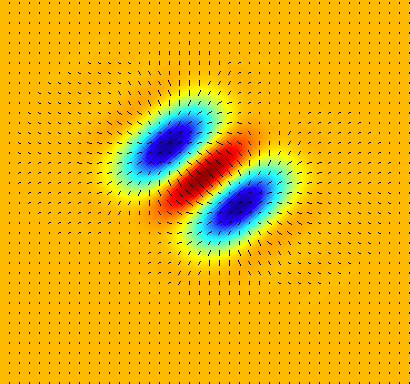
\includegraphics[width=10.cm]{FIG/fig_ecur.png}
}}
\end{figure}}

 
\newpage

\includeonly{cover,foreword,install}

\begin{document}
\maketitle
\newpage
$ $ 
\newpage
{\large
\voffset 0cm
\pagenumbering{roman}
\addcontentsline{toc}{chapter}{Contents}
\tableofcontents

 
\pagenumbering{arabic}
\clearpage



\newpage
\thispagestyle{empty}
$ $
\newpage

{\Huge \bf Acknowledgments}\label{forewd}\\
\vspace{1cm}
\markboth{Acknowledgments}{Acknowledgments}
\addcontentsline{toc}{chapter}{Acknowledgments}

The authors of this software package would like to express their 
gratitude to all of their colleagues who have made this work  
possible through various contributions. 
We are especially thankful to our direct collaborators with whom we 
have been working for years on problems in statistics and data 
analysis in astrophysics and cosmology: Nabila Aghanim, Jacques Delabrouille, David Donoho, 
Olivier Forni, Jiashun Jin, Mai Nguyen and Guillaume Patanchon.
This package is a compilation of the algorithms and methods which were 
developed and/or used successfully in a number of applications 
reported in the following publications: \\
\begin{itemize}
\item[$\bullet$]{ \textbf{ Multi--Detector Multi--Component spectral matching and applications for CMB data analysis}, J. Delabrouille, J.-F. Cardoso and G. Patanchon, \emph{Monthly Notices of the Royal Astronomical Society}, 2003, vol. 346, n. 4, pp. 1089-1102 }
\item[$\bullet$]{ \textbf{ Detecting Cosmological non-Gaussian Signatures by Multi-scale Methods}, J.-L. Starck and N. Aghanim and O. Forni, \emph{Monthly Notices of the Royal Astronomical Society}, 2004, vol. 416, n. 4, pp. 9-17 }
\item[$\bullet$]{ \textbf{ Cosmological Non-Gaussian Signatures Detection: Comparison of Statistical Tests}, J. Jin,  J.-L. Starck,  D.L. Donoho,  N. Aghanim and O. Forni, \emph{EURASIP Journal of Applied Signal Processing},  vol. 2005, n.15, pp 2470-2485, 2005.}
\item[$\bullet$]{ \textbf{ Blind Component Separation in Wavelet Space: Application to {CMB} Analysis}, Y. Moudden and J.-F. Cardoso and J.-L. Starck and J. Delabrouille, 
\emph{EURASIP Journal of Applied Signal Processing}, vol. 2005, n. 15, pp 2437-2454, 2005.}
\item[$\bullet$]{ \textbf{ Wavelets, Ridgelets and Curvelets on the Sphere},  J.-L. Starck,  P. Abrial, Y. Moudden and M. Nguyen, \emph{Astronomy and Astrophysics}, 2005, to appear}
\item[$\bullet$]{ \textbf{ Sunyaev-Zeldovich cluster reconstruction in multiband  bolometer camera surveys}, S. Pires, J.-B. Juin, D. Yvon, Y. Moudden, S. Anthoine and E. Pierpaoli, submitted to \emph{Astronomy and Astrophysics}, June 2005, available at: \\
 http://arxiv.org/pdf/astro-ph/0508641}\\
\end{itemize}

Other colleagues we would like to acknowledge include:
Bedros Afeyan, Jerome Bobin, Emmanuel Candes, Pierre-Fran{\c{c}}ois Honor\'e, Ludovic Poupard, 
Philippe Querre, Sandrine Pires, Ryad Sehil and Patricio Vielva.

\newpage
\thispagestyle{empty}
$ $
\newpage




\chapter{{\isap}  Introduction and Installation}
\label{ch_install}
\markright{Installation}

 
\section{Introduction to {\isap} }

{\isap} is a collection of packages, in IDL and C++, related to sparsity and its application in astronomical data analysis
(the IDL software (\texttt{http://www.idl-envi.com}) is analogous to Matlab and is very widely used in astrophysics and in medical imaging). 
 The C++ routines can be used independently of IDL.  The library is available via the web site:\\ \\
{ \centerline{\texttt{http://www.cosmostat.org/isap.html }}}\\
\\
It contains the following packages:
\begin{itemize}
 \item{\Large \bf  {Sparse2D V1.0: }} {  \bf  {Sparsity for 1D and 2D data set. }} \\
 IDL and C++ code, allowing sparse decomposition, denoising and deconvolution.

 \item{\Large \bf  {MSVST V1.0: }} {  \bf  {Multi-Scale Variance Stabilizing Transform (MSVST) for 1D and 2D data set.}} \\
 IDL and C++ code for Poisson noise removal.
 
 \item{\Large \bf  {MRS V3.2: }} {  \bf  {MultiResolution on the Sphere.}} \\
  IDL and C++ code for sparse representation on the sphere.

 \item {\Large \bf  {SparsePOL V1.1:}}   {  \bf  {Polarized Spherical Wavelets and Curvelets.}}  \\
 IDL code for sparse representation of polarized data on the sphere.
 
 \item {\Large \bf {MRS-MSVSTS   V1.1:}}  { \bf  {Multi-Scale Variance Stabilizing Transform on the Sphere.}} \\
  IDL code for Poisson noise removal and deconvolution on mono-channel and multichannel spherical data.

  \item{\Large \bf  {SparseGal V1.0: }} {  \bf  {Sparsity for galaxies survey analysis.}} \\
 IDL code, with two subpackages:
 \begin{itemize}
 \item ISW V1.0:  Integrated Sachs-Wolfe effect detection.
 \item DarthFader V1.0: Spectroscopic Redshift Estimation using sparsity.
 \end{itemize}
  \item{\Large \bf  {SparseCMB V1.0: }} {  \bf  {Sparsity for CMB data analysis.}}  \\
 IDL and C++ code.
 \end{itemize}

\section{IDL Installation}

A set of routines has been developed in IDL. Starting IDL using the script program {\em isap.pro} allows the user 
to get the sparse IDL astronomical data analysis environment, and all routines described in the following can be called. 
An online help facility is also available by invoking the {\em isaph} program under IDL.

Then, installing the {\isap} package simply requires adding some lines in your environment profile:
\begin{itemize}
\item[$\bullet$] {define the environment variable \textbf{ISAP}}  
\begin{verbatim}
setenv ISAP /home/user/ISAP
\end{verbatim}
 \item[$\bullet$]{define the alias \textbf{isap}}  
\begin{verbatim}
alias isap 'idl $ISAP/idl/isap.pro  $ISAP/idl/compile_healpixfile' 
\end{verbatim}
If the Healpix package is not installed, then replace the previous command with
\begin{verbatim}
alias isap 'idl $ISAP/idl/isap.pro' 
\end{verbatim}
In this case, packages MRS, MRSP, MRS-MSVST  will not be active.

\end{itemize}
Then the command "isap" will start the IDL session using the {\isap} environment. 


\section{\projmrs package}
 
The \mrs package, included in  {\isap}, requires IDL (version 6.0 or later) and HEALPix (version 2.0 or later) to be installed. The HEALPix environment 
variable \textbf{HEALPix} is expected to be defined. HEALPix is available at:\\ \\
{\centerline{\texttt{http://sourceforge.net/projects/healpix}}}\\

 HEALPix binaries must be in the user path.
  
 \projmrs  contains also C++ programs that can be used from IDL or directly from a terminal session. It has been tested using gcc-4.4.1. C++ is not necessary, but for some applications
 such as inpainting, C++ routines are much faster. To compile C++ routine, do the following commands:
\begin{itemize}
\item[$\bullet$] {go the \textbf{iSAP} directory }  
\begin{verbatim}
cd  $ISAP/cxx/mrs/build
\end{verbatim} 
 \item[$\bullet$]{build the makefile}  
\begin{verbatim}
./cmake .. 
\end{verbatim}
\item[$\bullet$]{run the makefile}  
\begin{verbatim}
make
\end{verbatim}
\item[$\bullet$]{copy the created binaries to the \textbf{iSAP} binary directory}
\begin{verbatim}
make install
\end{verbatim}
\item[$\bullet$]{set the IDL global variable ISAPCXX equal to 1 in the file  \textbf{\$iSAP}/isap.pro or on the user command line after being in the IDL-iSAP environment. }
\begin{verbatim}
ISAP>  ISAPCXX=1
\end{verbatim}
\end{itemize}

 Simular installation procedures must be done for each C++ package available in  \textbf{\$iSAP/cxx}.
 
\subsection{Input Data}
Most of the functions of \mrs package are working with spherical maps either as input or as output variables. The maps could be in 
two possible kind of formats: the first one which will be recognized by all functions is the HEALPix format. This format allows 
two kind of pixel order in the data array called NESTED and RING. Unless stated, \mrs functions will work only with NESTED maps. 
Conversions between NESTED and RING schemes could be done with the function "REORDER" from HEALPix package. 

The second format which  is recognized by some functions of \mrs package, but not all, is the GLESP format. In IDL, the variable for an image in GLESP format 
is an IDL structure. The \mrs package includes the file "mrs\_glesp.pro" which contains several functions for working with GLESP images 
especially the functions "healpix2glesp" and "glesp2healpix" which are used for the conversions between Healpix and GLESP format.
To use the GLESP image format, GLESP library, available at {\texttt{http://www.glesp.nbi.dk}, must be installed, and the environment variable \textbf{GLESP}
must be initialized to the correct path.

\subsection{Global IDL \mrs Variable}
Four global \mrs variables, defined in the file "isap.pro", are available, and can be changed by the user.
\begin{itemize}
\item HealpixCXX: default is 1. By default, \mrs uses HEALPix C++ programs to compute the spherical harmonic coefficients. 
If HealpixCXX is set to 0, \mrs will call the HEALPix  Fortran programs. We recommend to keep HealpixCXX equal to 1. Fortran option
will not be supported in the future.
\item DEF\_ALM\_FAST: default is 1. By default, spherical harmonic coefficients are calculated with floating values. This is faster and requires less
memory, but is not as accurate than using double. Set DEF\_ALM\_FAST to zero to make all calculation with double.
\item DEF\_ALM\_NITER: default is 10. This variable is only used when DEF\_ALM\_FAST is equal to zero. DEF\_ALM\_NITER is the number of iterations
used by HEALPix to compute the spherical harmonic coefficients. In the fast mode (default mode), there is no iteration.
\item DEF\_NORM\_POWSPEC: default is 0. If DEF\_NORM\_POWSPEC is set to 1, the command "mrs\_powspec" will return a normalized power spectrum, 
such that a map containing a Gaussian noise with variance 1 will have a power spectrum equal to 1. 
\item ISAPCXX: Default is 0:  If the  \textbf{iSAP}  C++ code has been compiled, it is recommended to set it to 1. When it is equal to 1, then spherical harmonic transform
and recontruction are done using the \textbf{MRScxx} binaries instead of Healpix binaries. 
\end{itemize}


\section{\projpol package}
The {\pol}  package, included in  {\isap}, requires IDL (version 6.0 or later), HEALPix (version 2.0 or later), and \projmrs to be installed.


 

\part{\projmrs: \defprojmrs}


\chapter{Multiscale Entropy Theory}
\label{ch_entrop}
\index{entropy}
\section{Entropy and Image Restoration}

\subsection{Introduction}

The term ``entropy'' is due to Clausius (1865), and the concept of 
entropy was introduced by Boltzmann into statistical mechanics
in order to measure the number of microscopic ways that a given macroscopic
state can be realized. Shannon (1948) \cite{ima:shannon48} founded the mathematical theory of
communication when he suggested that the information gained in a 
measurement depends on the number of possible outcomes out of 
which one is realized. Shannon also suggested that 
the entropy can be used for maximization of the bit transfer rate under
a quality constraint. Jaynes (1957) \cite{entropy:jaynes57} 
proposed to use the entropy measure
for radio interferometric image deconvolution,  in
order to select between a set of possible solutions that which contains the
minimum of information or, following his entropy definition, that 
which has maximum entropy. In principle, the solution verifying such 
a condition should be the most reliable. A great deal of work has been 
carried out 
in the last 30 years on the use of the entropy for the general problem
of data filtering and deconvolution 
\cite{entropy:ables74,entropy:bontekoe94,entropy:burg67,entropy:frieden75,entropy:gull91,entropy:narrayan86,starck:pan96,entropy:skilling89,entropy:weir92,entropy:djafari94,entropy:djafari98}. 

Traditionally information and entropy are determined from events and the
probability of their occurrence.  Signal and noise are basic building-blocks 
of signal and data analysis in the physical sciences.  Instead of the 
probability of an event, we are led to consider the probabilities of our
data being either signal or noise. 

Observed data $Y$ in the physical sciences 
are generally corrupted by noise, which is often additive and which 
follows in many cases a Gaussian distribution, a Poisson distribution, or
a combination of both.  Other noise models may also be considered.
 Using Bayes' theorem to evaluate the probability distribution of the 
realization of the original signal $X$,
knowing the data $Y$, we have
 
\begin{eqnarray}
 \mathrm{p}(X|Y) = \frac{\mathrm{p}(Y|X).\mathrm{p}(X)}{\mathrm{p}(Y)}
\label{eqn_bayes}
\end{eqnarray}
$\mathrm{p}(Y|X)$ is the conditional probability distribution of getting the data 
$Y$ given an original signal $X$, i.e.\ it represents the distribution 
of the noise. It is given, in the case of uncorrelated Gaussian 
noise with variance $\sigma^2$, by:
\begin{eqnarray}
 \mathrm{p}(Y|X) = \mathrm{exp} \left\{
-\sum_{pixels} \frac{ (Y-X)^2}{2{\sigma}^2} \right\}
\label{eqn_proba}
\end{eqnarray}
The denominator in  equation \ref{eqn_bayes} is independent of $X$ and
 is considered as a constant (stationary noise). 
$\mathrm{p}(X)$ is the a priori distribution 
of the solution $X$. In the absence of any information on the solution 
$X$ except its positivity, a possible course of action 
is to derive the probability
of $X$ from its entropy, which is defined from information theory.

The main idea of information theory \cite{ima:shannon48} is to establish
a relation between the received information and the probability of
the observed event \cite{ima:bijaoui84}. If we note ${\cal I}(E)$ the information
related to the event $E$, and $p$ the probability of this
event happening, then we consider that
\begin{eqnarray}
%\cal{I}(E) =    f(p)       
{\cal I}(E) = f(p)
\end{eqnarray}

Then we assume the two following principles:
\begin{itemize}
\item The information is a decreasing function of the probability. This 
implies that the more information we have, the  less will be the probability 
associated with one event.
\item Additivity of the information. If we have two independent events 
$E_1$ and $E_2$, the information ${\cal I}(E)$ associated with the happening
of both is equal
to the addition of the information of each of them.
\begin{eqnarray}
{\cal I}(E) = {\cal I}(E_1) + {\cal I}(E_2)
\end{eqnarray}
\end{itemize}

Since $E_1$ (of probability $p_1$) and $E_2$ (of probability $p_2$) are 
independent, then the probability of both happening is equal to the
product of $p_1$ and $p_2$.  Hence
\begin{eqnarray}
f(p_1 p_2) = f(p_1) + f(p_2) 
\end{eqnarray}

Then we can say that the information measure is
\begin{eqnarray}
{\cal I}(E) = k \ln(p)
\end{eqnarray}
where k is a constant. Information must be positive, and $k$
is generally fixed at $-1$.

Another interesting measure is the mean information which is denoted
\begin{eqnarray}
H = - \sum_i p_i \ln(p_i)
\end{eqnarray}
This quantity is called the entropy of the system and was established by 
Shannon in 1948 \cite{ima:shannon48}.

This measure has several properties:
\begin{itemize}
\item It is maximal when all events have the same probability 
$p_i = 1/ N_e$ ($N_e$ being the number of events), and is equal to 
$\ln(N_e)$. It is in this 
configuration that the system is the most undefined.
\item It is minimal when one event is sure. In this case, the system is 
perfectly known, and no information can be added.
\item The entropy is a positive, continuous, and symmetric function.
%\item The mean information, obtained in two steps, can be added.
\end{itemize}

If we know the entropy $H$ of the solution (the next section 
describes different ways to calculate it), 
we derive its probability by
\begin{eqnarray}
\mathrm{p}(X) = \mathrm{exp}(- \alpha H(X))
\label{info_prop}
\end{eqnarray}

Given the data, the most probable image is obtained by maximizing
$\mathrm{p}(X|Y)$. Taking the logarithm of equation \ref{eqn_bayes}, we 
thus need to maximize
\begin{eqnarray}
 \ln (\mathrm{p}(X|Y))  = - \alpha  H(X) + \ln(\mathrm{p}(Y|X)) - 
\ln(\mathrm{p}(Y))
\end{eqnarray}
The last term is a constant and can be omitted.
Then, in the case of Gaussian noise, the solution is found by minimizing 
\begin{eqnarray}
J(X) = \sum_{pixels} \frac{{(Y-X)}^{2}}{2 {\sigma}^{2}} + {\alpha} H(X)
= \frac{{\chi}^2}{2} + {\alpha} H(X)
\label{eqn_j1}
\end{eqnarray}
which is a linear combination of two terms: the entropy of the signal,
and a quantity corresponding to ${\chi}^2$ in statistics measuring the
discrepancy between the data and the predictions of the model.
$\alpha$ is a parameter that can be viewed alternatively as 
a Lagrangian parameter or a value fixing the relative weight between 
the goodness-of-fit and the entropy H. 

For the deconvolution problem, the object-data relation is given by the
convolution
\begin{eqnarray}
Y = P * X
\end{eqnarray}
where $P$ is the point spread function, and the solution is found (in the case
of Gaussian noise) by minimizing
\begin{eqnarray}
J(X) = \sum_{pixels} \frac{{(Y-P*X)}^{2}}{2 {\sigma}^{2}} + {\alpha} H(X)
\end{eqnarray}

The way the entropy is defined is fundamental, because from its definition
will depend the solution. The next section discusses the different approaches 
which have been proposed in the past.

\clearpage
\newpage

\subsection{The concept of entropy}
\label{sect_entr}
We wish to estimate an unknown probability density $p(X)$ of the data.
 Shannon \cite{ima:shannon48}, in the framework of the information 
 theory, has defined the entropy of an image $X$ by 
\begin{eqnarray}
H_s(X) = - \sum_{k=1}^{N_b} p_k \log p_k
\end{eqnarray}
where  $X=\left\{X_1,.. X_N \right\}$ is an image 
containing integer values, $N_b$ is number of possible values which can 
take a given pixel $X_k$ 
(256 for a 8 bits image), and 
 $p_k$ values are derived the histogram of $X$:
\begin{eqnarray}
p_k = {  \mbox{\#} X_j = k \over  N} 
\end{eqnarray}
$\mbox{\#} X_j = k $ giving the number of pixels  $X_j = k$.

If the image contains floating values, it is possible to
to build up the histogram $L$ of values $L_i$, using
a suitable interval $\Delta$, counting up how many times $m_k$ each interval
$(L_k, L_k + \Delta)$ occurs among the N occurrences. Then the probability
that a data value belongs to an interval $k$ is $p_k = \frac{m_k}{N}$, and
each data value has a probability $p_k$.  

The entropy is minimum and equal to zero when the signal is flat, and
increases when we have some fluctuations. Using this entropy in 
equation~\ref{eqn_j1} leads to minimize:
\begin{eqnarray}
J(X) = \frac{{\chi}^2}{2} + {\alpha} H_s(X)
\label{eqn_j2}
\end{eqnarray}
It is a minimum entropy restoration method.
 
The trouble with this approach is that, because the number of occurrences is
finite, the estimate $p_k$ will be in error by an amount proportional
to $m_k^{-\frac{1}{2}}$~\cite{entropy:frieden91}. The error becomes significant when
$m_k$ is small. Furthermore this kind of entropy definition is not
easy to use for signal restoration, because the gradient of 
equation~\ref{eqn_j2} is not easy to compute. 
For these reasons, other
entropy functions are generally used. The main ones are:
\begin{itemize}
\item Burg \cite{entropy:burg67}:
\begin{eqnarray}
H_b(X) = -\sum_{k=1}^N \ln(X_k) 
\end{eqnarray}
\item Frieden \cite{entropy:frieden75}:
\begin{eqnarray}
H_f(X) = -\sum_{k=1}^N X_k \ln(X_k)
\end{eqnarray}
\item Gull and Skilling \cite{entropy:gull91}:
\begin{eqnarray}
H_g(X) = \sum_{k=1}^N  X_k - M_k - X_k \ln({X_k \over M_k})
\end{eqnarray}
where $M$ is a given model, usually taken as a flat image
\end{itemize}
where $N$ is the number of pixels, and $k$ represents an index pixel.

Each of these entropies can be used, and they correspond to different
probability distributions that one can associate with 
an image \cite{entropy:narrayan86}.
(See \cite{entropy:frieden75,entropy:skilling89} for descriptions).
The last definition of the entropy has the advantage of having a zero
 maximum when $X$ equals the model $M$. 
All of these entropy measures are negative (if $X_k > 1$), 
and maximum when the image is flat.
They are negative because an offset term is omitted which has no importance
for the minimization of the functional. The fact that we consider that
a signal has maximum information value when it is flat is evidently
a curious way to measure information. A consequence is that we must
now maximize the entropy if we want a smooth solution, and
the probability of $X$ 
must be redefined by:
\begin{eqnarray}
\mathrm{p}(X) = \mathrm{exp}(\alpha H(X))
\end{eqnarray}
The sign has been inverted
(see equation~\ref{info_prop}), which is natural if we want the best
solution to be the smoothest. These three entropies, above, lead to the 
Maximum Entropy Method method (MEM), for which the 
solution is found by minimizing 
(for Gaussian noise)
\begin{eqnarray}
J(X) = \sum_{k=1}^N \frac{{(Y_k-X_k)}^{2}}{2 {\sigma}^{2}} - {\alpha} H(X)
\label{eqn_j3}
\end{eqnarray}

These different entropy functions  which have
been proposed for image restoration have the property of being maximal when
the image is flat, and of decreasing when we introduce some information.
So minimizing the information is equivalent to maximizing the entropy, and
this has led to the well known Maximum Entropy Method (MEM). For the Shannon
entropy (which is obtained from the histogram of the data), 
this is the opposite. The entropy is null for a flat image, and increases
when the data contains some information. So, if the Shannon entropy were 
used for restoration, this would lead to a Minimum Entropy Method.

In 1986, Narayan and Nityanda \cite{entropy:narrayan86} 
compared several entropy functions,
 and finally 
concluded by saying that all were comparable if they have good
properties, i.e.\ they enforce positivity, and they have a negative 
second derivative which discourages ripple. They showed also that 
results varied strongly with the background level, and
that these entropy functions produced poor results
for negative structures, i.e.\ structures under the background level
(absorption area in an image, absorption band in a spectrum, etc.), and 
compact structures in the signal.
The Gull and Skilling entropy gives rise to  
the difficulty of estimating a model.
Furthermore it has been shown \cite{entropy:bontekoe94} 
that the solution is dependent on this choice.

The determination of the $\alpha$ parameter is also not an easy task and in 
fact it is a very serious problem facing the maximum entropy method.
In the historic MAXENT algorithm of Skilling and Gull, the choice of $\alpha$ 
is such that it must satisfy the ad hoc constraint $\chi^2=N$ when 
the deconvolution is achieved, $N$ being
 the number of degrees of freedom of the system i.e.\ the number of pixels 
in image deconvolution problems.
But this choice systematically leads to an under-fitting of the data 
 \cite{entropy:titterington85} which is clearly apparent for imaging problems 
with little blurring. In reality, the $\chi^2$ statistic is expected to 
vary in the range $N\pm\sqrt{2N}$ from one data realization to another.
 In the Quantified Maximum Entropy point of view \cite{entropy:skilling89}, the 
optimum value of $\alpha$ is determined by including its probability 
P($\alpha$) in Bayes' equation and then by maximizing the marginal 
probability of having $\alpha$, knowing the data and the model $m$.
 In practice, a value of $\alpha$ which is too large gives a resulting image 
which is too regularized
\index{regularization}
with a large loss of resolution.  A value which is too small
leads to a poorly regularized solution showing unacceptable artifacts. 
Taking a flat model of the prior image softens the discontinuities 
which may appear unacceptable for astronomical images often containing 
stars and other point-like objects. Therefore the basic maximum entropy 
method appears to be not very
appropriate for this kind of image which contains high and low spatial 
frequencies 
at the same time. Another point to be noted 
is a ringing effect of the maximum entropy method algorithm,
producing artifacts around bright sources.

 To solve these problems while still using the maximum entropy concept, some 
enhancements of the maximum entropy method have been proposed.
Noticing that neighboring pixels of reconstructed images with MAXENT 
could have values differing a lot in expected flat regions \cite{entropy:charter89}, 
Gull and Skilling introduced the concepts of hidden image $S$ and intrinsic 
 correlation function $C$ (Gaussian or cubic spline-like) 
in the Preblur MAXENT algorithm.
\index{maximum entropy method}
\index{MEM}
\index{intrinsic correlation function}

 The ICF describes a minimum scale length of correlation in the desired 
image $O$ which is achieved by assuming that
\begin{eqnarray}
 O=C*S
\end{eqnarray}
This corresponds to imposing a  
minimum resolution on the solution $O$. 
Since the hidden space image $S$ is not 
spatially correlated, this can be regularized by the entropy 
\begin{eqnarray}
H_g(h)=\sum_{k=1}^N  S_k - M_k - S_k \ln(\frac{S_k}{M_k})
\end{eqnarray}

Since in astronomical images many scale lengths are present, the 
{\it Multi-channel Maximum Entropy Method}, developed by Weir 
\index{maximum entropy method}
\index{MEM}
\cite{entropy:weir91,entropy:weir92}, uses a set of 
ICFs having different scale lengths, each defining a channel. The 
visible-space image is now formed by a weighted sum of 
 the visible-space image
channels $O_j$:
   
\begin{eqnarray}
  O= \sum_{j=1}^{N_c} p_j O_j
\end{eqnarray}
where $N_c$ is the number of channels.
Like in Preblur MAXENT, each solution $O_j$ is supposed to be the result of the
convolution between a hidden image $S_j$ with a low-pass filter (ICF) $C_j$:
\begin{eqnarray}
O_j = C_j * S_j
\end{eqnarray}

But such a method has several drawbacks:
\begin{enumerate}
\item The solution depends on the width of the ICFs \cite{entropy:bontekoe94}.
\item There is no rigorous way to fix the weights $p_j$ \cite{entropy:bontekoe94}.
\item The computation time increases linearly with the number of pixels.
\item The solution obtained depends on the choice of the models $M_j$ 
($j = 1 \dots N_c$) which were chosen independently of the channel.
\end{enumerate}
\index{intrinsic correlation function}

In 1993, Bontekoe et al.\ \cite{entropy:bontekoe94} used a special application 
of this method which 
they called Pyramid Maximum Entropy on infrared image data.
\index{pyramid}
The pyramidal approach allows the user to have constant ICF width, and the 
computation time is reduced. It is demonstrated \cite{entropy:bontekoe94} that
all weights can be fixed ($p_j = 1$ for each channel). 

This method eliminates the first three drawbacks, and
gives better reconstruction of the sharp 
and smooth structures. But in addition 
to the two last drawbacks, a new one is added:
as the images $O_j$ have different sizes (due to the pyramidal approach),
\index{pyramid}
the solution $O$ is built by duplicating the pixels of 
the subimages $O_j$ of each channel. This procedure is known to produce 
artifacts due to the  appearance of high frequencies which are
incompatible with the 
real spectrum of the true image $\hat{O}$.

However this problem can 
be easily overcome by duplicating the pixels before convolving with the ICF, 
or expanding the channels using linear 
interpolation. Thus the introduction of the ``pyramid of resolution'' has 
solved some problems and brought lots of improvements to the classic maximum
entropy method, but has also raised other questions. In order to derive the
model from a physical value, Pantin and Starck \cite{starck:pan96} 
introduced the wavelet 
transform, and defined entropy as follows:
\begin{eqnarray}
H(O) =  \frac{1}{\sigma_I^2}\sum_{j=1}^l \sum_{k=1}^{N_j} \sigma_j( w_{j,k}- M_{j,k}- |w_{j,k}|\ln{\frac{|w_{j,k}|}{M_{j,k}}})
\label{eqn_entr}
\end{eqnarray}
where $\sigma_I$ is the noise standard deviation in the data, $l$ is the number of scales, and
$N_j$ is the number of samples in the band $j$
($N_j = N$ for the \`a trous algorithm). 
The multiscale entropy is the sum of the entropy at each scale.

The coefficients $w_{j,k}$ are wavelet coefficients, and we 
take the absolute value of $w_{j,k}$ in this definition because the  
values of $w_{j,k}$ can be positive or negative, and a negative signal 
contains also some information in
the wavelet transform. 

The advantage of such a definition of entropy is
 the fact we can use previous work concerning the wavelet transform and
image restoration \cite{starck:mur95_2,starck:sta94_1,starck:sta94_4}. 
The noise behavior has already been studied in the wavelet transform 
and we can estimate the standard deviation of the noise $\sigma_j$ 
at scale $j$. These estimates can be naturally introduced in our 
models $m_j$
\begin{eqnarray}
M_{j,k} = k_{m} \sigma_j
\end{eqnarray}
 The model $M_j$ at scale $j$ represents 
the value taken by a wavelet coefficient in the absence of any relevant
 signal and, in  practice, it must be a small value compared to 
any significant signal value.
Following the Gull and Skilling procedure, we take $M_j$ as a fraction of the 
noise because the value of 
$\sigma_j$ can be considered as a sort of physical limit under which a signal 
cannot be distinguished from the noise ($k_m = \frac{1}{100}$).

\subsection{Conclusion}
\label{sect_5pt}

As described above, many studies   
have been carried out in order to improve the functional to be minimized.
But the question which should be raised is: what is a good entropy for 
signal restoration?

Trying to answer, this corresponds to asking what is the information
in the signal. We first assume that a signal $X$ can be decomposed in
several components:
\begin{eqnarray}
 X = S + B + N
\end{eqnarray}
where $S$ is the signal of interest, $B$ lis the background, and $N$  the noise.

The entropy should verify the following criteria \cite{starck:sta98_2}:
{\bf
\begin{enumerate}
\item The information in a flat signal is zero ($S=0$, $N=0$ et $B=\mathrm{Cst}$). 
\item The amount of information in a signal is independent of the background
($H(X)$ is independent of $B$).
\item The amount of information is dependent on the noise 
($H(X)$ is dependent of $N$). 
A given signal $X$ doesn't furnish the  same information if 
the noise $N$ is high or small.
\item The entropy must work in the same way for a pixel which
has a value $B + \epsilon$, and
for a pixel which has a value $B - \epsilon$.
$H(X)$ must be a function of the absolute value of $S$ instead of $S$.
\item The amount of information is dependent on the correlation in the signal.
If the signal $S$  presents large features above the noise, it contains
a lot of information. By generating a new set of  data from $S$, by 
randomly taking the pixel values in $S$, the large features will
evidently disappear, and this new signal will contain less information.
But the pixel values will be the same as in $S$.
\end{enumerate}
}
% \begin{figure}[htb]
% \centerline{
% \hbox{
% \psfig{figure=lenna256.ps,bbllx=1.8cm,bblly=12.9cm,bburx=14.5cm,bbury=25.5cm,width=8cm,height=8cm,clip=}
% \psfig{figure=scrambled_lenna.ps,bbllx=1.8cm,bblly=12.9cm,bburx=14.5cm,bbury=25.5cm,width=8cm,height=8cm,clip=}
% }}
% \caption{Lena image (left) and the same data distributed differently (right). 
% These
% two images have the same entropy, using any of the standard entropy methods.}
% \label{fig_lenna}
% \end{figure}
\begin{figure}[h]
\centerline{
\vbox{
\hbox{
\psfig{figure=fig_saturn.ps,bbllx=1.7cm,bblly=12.9cm,bburx=11.2cm,bbury=25.6cm,width=9.cm,height=12.3cm,clip=}
\psfig{figure=fig_saturn_scramble.ps,bbllx=1.7cm,bblly=12.9cm,bburx=11.2cm,bbury=25.6cm,width=9.cm,height=12.3cm,clip=}
% \vspace{21cm}
}
}}
\caption{Saturn image (left) and the same data distributed differently (right). 
These
two images have the same entropy, using any of the standard entropy 
definitions.}
\label{fig_saturn}
\end{figure}
 
Fig.~\ref{fig_saturn} illustrates the last point perfectly. 
The second image is obtained  by distributing randomly the Saturn image pixel 
values, and the standard entropy definitions  produce the same information
measurement for both images. The concept of information becomes really
subjective, or at least it depends on the application domain. Indeed, for 
someone who is
not involved in image processing, the second image contains 
{\em less} information
than the first one. For someone working on image transmission, it is clear
that the second image will require more bits for lossless transmission,
and from this point of view, he/she will consider that the second 
image contains
{\em more} information. Finally, for data restoration, all fluctuations
due to noise are not of interest, and do not contain relevant 
information. From this physical point of view, 
the standard  definition of entropy seems badly adapted to information 
measurement in signal restoration.

% \clearpage
% \newpage
  


\chapter{Multiscale Methods on the Sphere}
\label{ch_mms}
\index{Multiscale}

\section{Introduction}
\section{The Isotropic Undecimated Wavelet Transform}
\section{The Isotropic Pyramidal Wavelet Transform}
\section{The Ridgelet Transform}
\section{The Curvelet Transform}





  

\chapter{Data Restoration on the Sphere}
\label{ch_restore}
\index{Denoising}
\index{Filtering}

\label{sect_exp}
\section{Introduction}
\index{wavelet!denoising}
\index{curvelet!denoising}

Wavelets and Curvelets have been used successfully for image denoising \emph{via} non-linear filtering or 
thresholding methods \cite{starck:book02,starck:sta01_3}. Hard thresholding, for instance, consists in 
setting all insignificant coefficients (\emph{i.e.} coefficients with an absolute value below a given 
threshold) to zero. In practice, we need to estimate the noise standard deviation $\sigma_j$ in each band 
$j$ and a wavelet (or curvelet) coefficient $w_j$ is significant if $\mid w_j \mid > k \sigma_j$, where $k$ 
is a user-defined parameter, typically chosen between 3 and 5. The $\sigma_j$ estimation in band $j$ can be 
derived from simulations \cite{starck:book02}. Denoting $D$ the noisy data and $\delta$ the thresholding 
operator, the filtered data $\tilde D$ are obtained by : 
\begin{eqnarray}
 {\tilde D} =    {\cal R} \delta( {\cal T} D)
\end{eqnarray}
where ${\cal T}$ is the wavelet (resp. curvelet) transform operator and ${\cal R}$ is the wavelet (resp. curvelet) reconstruction operator. 


\section{Significant Wavelet Coefficients}
\label{ch_noise}
\subsection{Definition}
\index{noise}
\index{wavelet!significant coefficient}

In most applications, it is necessary to know if a wavelet coefficient is due to signal (i.e.\ it is significant) or to noise. 

The wavelet (resp. curvelet) transform yields a set of resolution-related views of the input image. 
A wavelet (resp. curvelet) band at level $j$ has coefficients given by $w_{j,k}$. If we obtain the 
distribution of the coefficient $w_{j,k}$ for each band of the decomposition, based on the noise, 
we can introduce a statistical significance test for this coefficient. This procedure is the classical 
significance-testing one. Let ${\cal H}_0$ be the hypothesis that the image is locally constant at scale $j$.  
Rejection of hypothesis ${\cal H}_0$ depends (for positive coefficient values) on:
\begin{eqnarray}
P = Prob(\mid w_{j,k} \mid \ < \ \tau \mid {\cal H}_0)  
\end{eqnarray}
The detection threshold, $\tau$, is defined for each scale. Given an estimation threshold, $\epsilon$, 
if $P = P(\tau) > \epsilon$ the null hypothesis is not excluded. Although non-null, the value of the 
coefficient could be due to noise. On the other hand, if $P < \epsilon$, the coefficient value cannot be due to 
the noise alone, and so the null hypothesis is rejected. In this case, a significant coefficient has been detected.

\subsection{Noise Modeling}
\index{noise}
\index{noise!Gaussian}
If the distribution of $w_{j,l}$ is Gaussian, with zero mean and standard deviation $\sigma_j$, we have the probability density
\begin{eqnarray}
p(w_{j,l}) = \frac{1}{\sqrt{2\pi} \sigma_j} e^{{- w_{j,l}^2}/2\sigma^2_j} 
\end{eqnarray}
Rejection of hypothesis ${\cal H}_0$ depends (for a positive coefficient value) on:
\begin{eqnarray}
P = Prob( w_{j,l} > W) = \frac{1}{\sqrt{2\pi} \sigma_j} \int^{+\infty}_{w_{j,l}} e^{-W^2/2\sigma^2_j} dW 
\end{eqnarray}
and if the coefficient value is negative, it depends on 
\begin{eqnarray}
P = Prob( w_{j,l} < W) = \frac{1}{\sqrt{2\pi} \sigma_j} \int^{w_{j,l}}_{-\infty} e^{-W^2/2\sigma^2_j} dW 
\end{eqnarray}

Given stationary Gaussian noise, it suffices to compare $w_{j,l}$ to 
\index{stationary signal}
$k \sigma_j$.  Often $k $ is chosen as 3, which corresponds approximately to $\epsilon = 0.002$.  
If $w_{j,l}$ is small, it is not significant and could be due to noise. If $w_{j,l}$ is large, it is significant:
\begin{eqnarray}
\begin{array}{l}
\mbox{ if }  \mid  w_{j,l} \mid \ \geq \ k \sigma_j \ \ \mbox{ then } w_{j,l}   \mbox{ is significant } \\ 
\mbox{ if }  \mid  w_{j,l} \mid \ < \ k \sigma_j \ \ \mbox{ then }  w_{j,l} \mbox{ is not significant }
\end{array}
\end{eqnarray}

So we need to estimate, in the case of Gaussian noise models, the noise standard deviation at each scale. 
These standard deviations can be determined analytically, but the calculations can become complicated.  

The appropriate value of $\sigma_j$ in the succession of wavelet planes is assessed from the standard deviation 
of the noise $\sigma_N$ in the original data $D$, and from study of the noise in the wavelet space. This study 
consists of simulating a data set containing Gaussian noise with a standard deviation equal to 1, and taking the 
wavelet transform of this data set. Then we compute the standard deviation $\sigma^e_j$ at each scale. We get a curve 
$\sigma^e_j$ as a function of $j$, giving the behavior of the noise in the wavelet space (Note that if we had used 
an orthogonal wavelet transform, this curve would be linear). Due to the properties of the wavelet (resp. curvelet) 
transform, we have $ \sigma_j = \sigma_N \sigma^e_j $. The noise standard deviation at scale $j$ of the data is equal 
to the noise standard deviation $\sigma_N$ multiplied by the noise standard deviation at scale $j$ of the simulated data.

\subsection{Automatic Estimation of Gaussian Noise}
\subsubsection{$k$-sigma clipping}
\index{sigma clipping}
\index{noise!sigma clipping}
\index{noise}
The Gaussian noise $\sigma_N$ can be estimated automatically in a data set $D$. This estimation is particularly important, 
because all the noise standard deviations $\sigma_j$ in the scales $j$ are derived from $\sigma_N$. Thus an error associated 
with $\sigma_N$ will introduce an error on all $\sigma_j$. Noise is therefore more usefully estimated in the high frequencies, 
where it dominates the signal. The resulting method consists first of filtering the data $D$ with an average filter or the 
median filter and subtracting from $D$ the filtered signal $F$: $S = D - F $. In our case, we replace $S$ by the first scale 
of the wavelet transform ($S = w_1$), which is more convenient from the computation time point of view. The histogram of $S$ 
shows a Gaussian peak around 0. A k-sigma clipping is then used to reject pixels where the signal is significantly large. 
We denote $S^{(1)}$ the subset of $S$ which contains only the pixels such that $\mid S_l \mid \ < k \sigma_S$, where $\sigma_S$ 
is the standard deviation of $S$, and $k$ is a constant generally chosen equal to 3. By iterating, we obtain the subset $S^{(n+1)}$ 
verifying $\mid S^{(n)}_l \mid \ < k \sigma_{S^{(n)}}$, where $\sigma_{S^{(n)}}$ is the noise standard deviation of $S^{(n)}$. 
Robust estimation of the noise $\sigma_1$ in $w_1$ (as $S = w_1$) is now obtained by calculation of the standard deviation of 
$S^{(n)}$ ($\sigma_1 = \sigma_{S^{(n)}}$). In practice, three iterations are enough, and accuracy is generally better than $5$\%.
$\sigma_N$ is finally calculated by: 
\be
\sigma_N = \frac{\sigma_1}{\sigma^e_1} = \frac{\sigma_{S^{(n)}} }{\sigma^e_1}
\ee


\subsection{Correlated Noise}
\index{median!median absolute deviation}
\index{MAD}
\index{noise!median absolute deviation}
\index{noise}
In this case, the data can be treated as for the Gaussian case, but the noise standard deviation $\sigma_j$ at scale $j$ 
is calculated independently at each scale. Two methods can be used: 
\begin{enumerate}
\item $\sigma_j$ can be derived from a k-sigma clipping method applied at scale $j$.
\item The median absolute deviation, MAD, can be used as an estimator of the noise standard deviation:
\begin{eqnarray}
\sigma_j = \mbox{median}( \mid w_j \mid ) / 0.6745
\end{eqnarray}
\end{enumerate}

\section{Thresholding}
Many filtering methods have been proposed in the last ten years. {\em Hard thresholding} consists of setting to 0 all 
wavelet coefficients which have an absolute value lower than a threshold $T_j$ (non-significant wavelet coefficient):
\begin{eqnarray}  \tilde w_{j,k} = 
\left\{ \begin{array}{ll} w_{j,k} &  \mbox{ if } \mid w_{j,k} \mid \geq T_j  \nonumber  \\ 

0 &  \mbox{ otherwise}  \end{array} \right. 
\end{eqnarray}
where $w_{j,k}$ is a wavelet coefficient at scale $j$ and at spatial position $k$. 

{\em Soft thresholding} consists of replacing each wavelet coefficient by the value $\tilde w$ where
\begin{eqnarray}  \tilde w_{j,k} = 
\left\{ \begin{array}{ll} sgn(w_{j,k}) ( \mid w_{j,k} \mid - T_j)    &  \mbox{ if } \mid w_{j,k} \mid \geq T_j \nonumber  \\ 
0 &  \mbox{ otherwise}  \end{array} \right. 
\end{eqnarray} 
This operation is generally written as:
\begin{eqnarray} 
 \tilde w_{j,k} = \mathrm{soft}( w_{j,k})  = sgn(w_{j,k}) ( \mid w_{j,k} \mid - T_j)_{+}
\end{eqnarray} 
where $(x)_{+} = MAX(0,x)$.

When the discrete orthogonal wavelet transform is used instead of the \`a trous algorithm, it is interesting to note
that the hard and soft thresholded estimators are solutions of the following minimization problems:
\begin{eqnarray*}
  \tilde w  =   \mathrm{arg}_w \min {1 \over 2} \parallel D - {\cal W}^{-1} w \parallel^2_{l^2} + 
 \lambda \parallel w \parallel^2_{l^0} & & \mbox{\bf   hard threshold} \nonumber \\
  \tilde w   =   \mathrm{arg}_w \min {1 \over 2} \parallel D - {\cal W}^{-1} w \parallel^2_{l^2} + 
 \lambda \parallel w \parallel^2_{l^1} & & \mbox{\bf   soft threshold}  
\end{eqnarray*}
where $D$ is the input data, ${\cal W}$ the wavelet transform operator, and $l^0$ indicates the limit of $l^\delta$ 
when $\delta \rightarrow 0$. This counts in fact the number of non-zero elements in the sequence.
\index{thresholding!hard}
\index{thresholding!soft}
\index{wavelet!hard threshold}
\index{wavelet!soft threshold}

As described before, in the case of Gaussian noise, $T_j = K \sigma_j$, where $j$ is the scale of the wavelet coefficient, 
$\sigma_j$ is the noise standard deviation at the scale $j$, and $K$ is a constant generally chosen equal to 3.

Other threshold methods have been proposed, like the {\em universal threshold} 
\index{universal threshold}
\index{SURE}
\index{thresholding!universal threshold}
\index{thresholding!SURE}
\cite{rest:donoho93_1,rest:donoho93_2}, or the SURE (Stein Unbiased Risk Estimate) method \cite{rest:donoho95},
but they generally do not yield as good results as the hard thresholding method based on the significant coefficients.  
For astronomical data, soft thresholding should never be used because it leads to a photometry loss associated with all 
objects, which can easily be verified by looking at the residual map (i.e.\ data $-$ filtered data). Concerning the 
threshold level, the universal threshold  corresponds to a minimum risk. The larger the number of pixels, the larger 
is the risk, and it is normal that the threshold $T$ depends on the number of pixels ($T = \sqrt{2\log n} \sigma_j$, 
$n$ being the number of pixels). The $K\sigma$ threshold corresponds to a false detection probability, the probability 
to detect a coefficient as significant when it is due to the noise. The $3\sigma$ value corresponds to 0.27 \% false detection.
 
\begin{figure*}
% 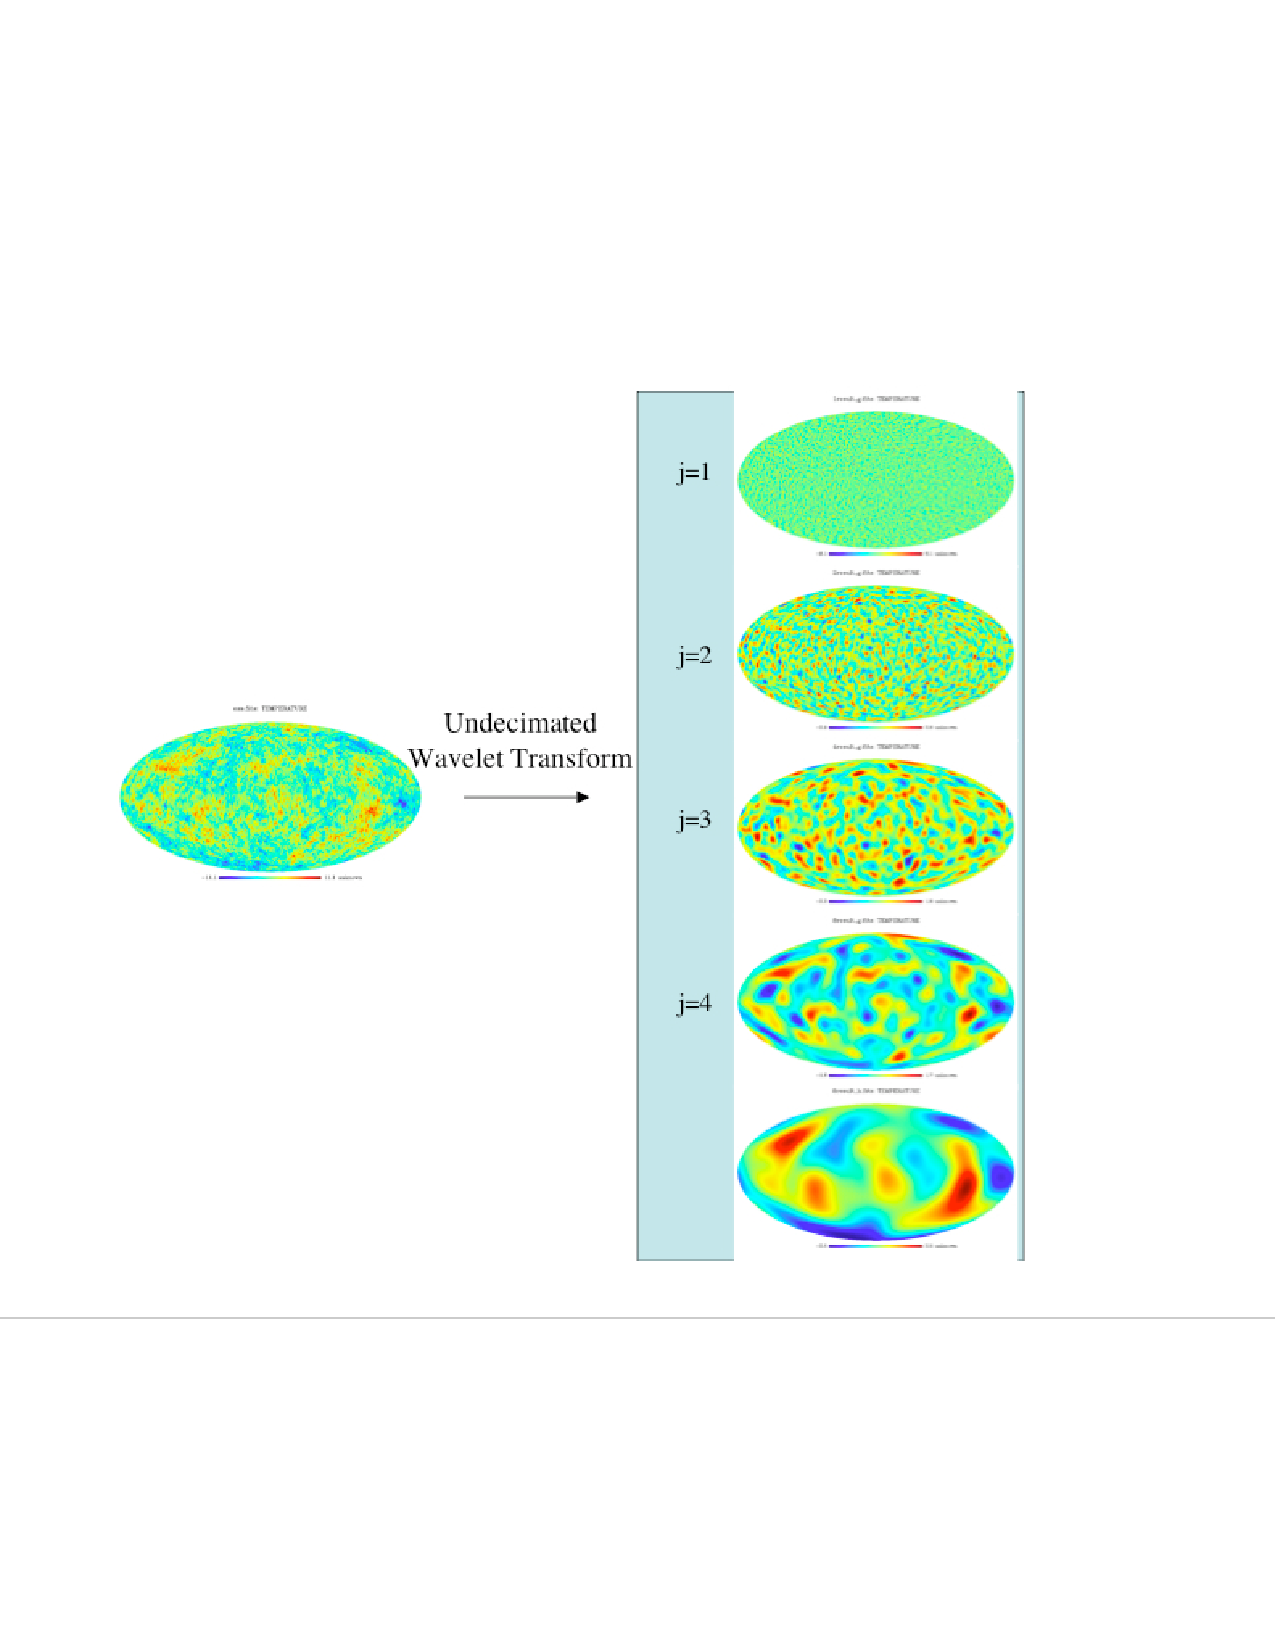
\includegraphics[height=8truecm,width=6truecm]{fig_uwt_sphere.pdf}
% 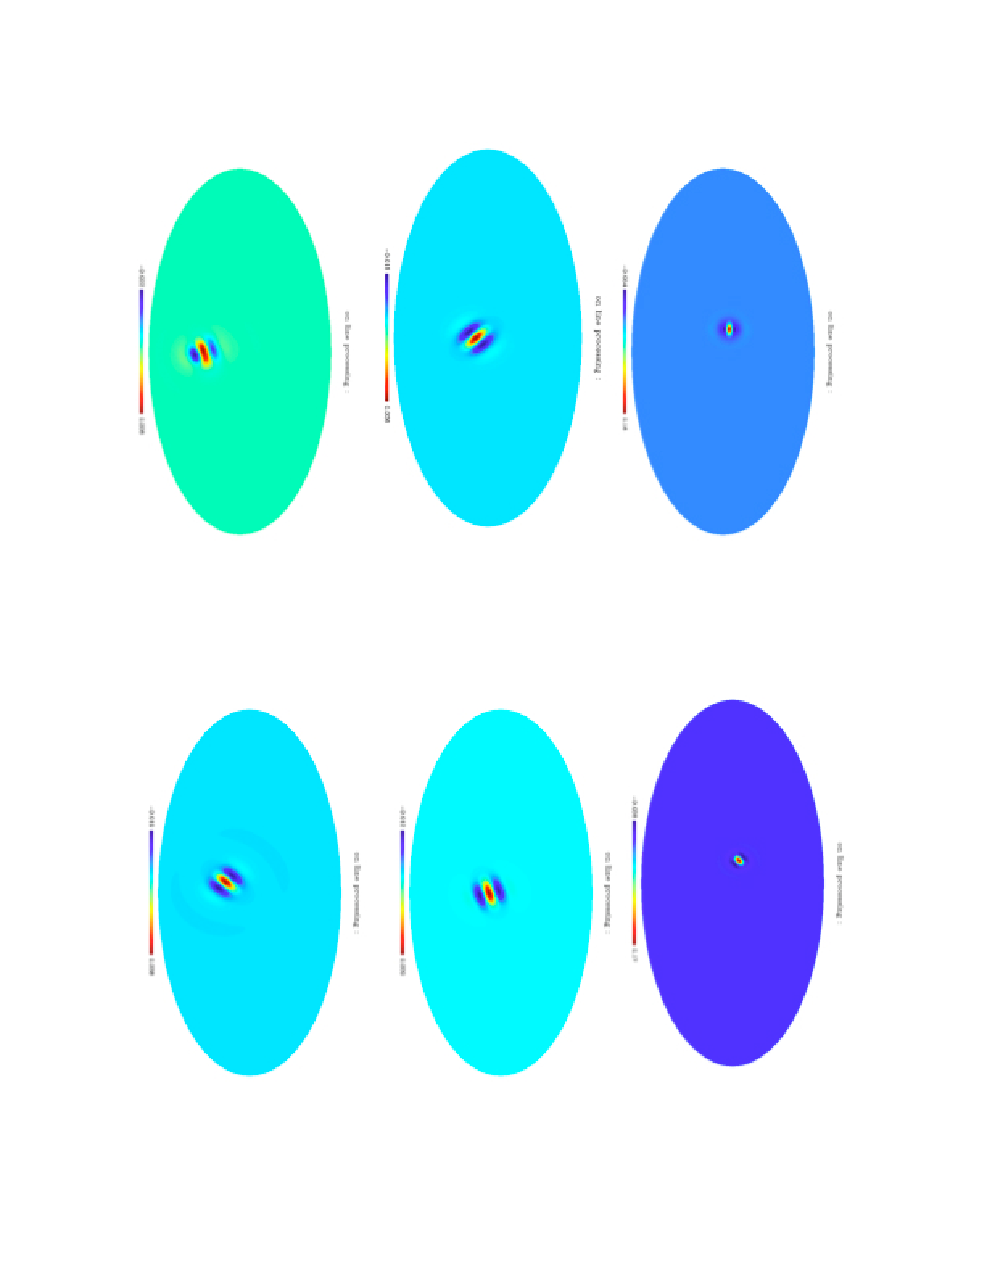
\includegraphics[height = 5 in]{fig_back_cur_sphere.pdf}
\vbox{
\centerline{
\hbox{
\psfig{figure=fig_synchrotron_bw.pdf,bbllx=0.5cm,bblly=9.5cm,bburx=20cm,bbury=20cm,width=8cm,height=4.5cm,clip=}
\psfig{figure=fig_synchrotron_noise5_bw.pdf,bbllx=0.5cm,bblly=9.5cm,bburx=20cm,bbury=20cm,width=8cm,height=4.5cm,clip=}
}}
\centerline{
\hbox{
\psfig{figure=fig_pwt5_synchrotron_noise5_bw.pdf,bbllx=0.5cm,bblly=9.5cm,bburx=20cm,bbury=20cm,width=8cm,height=4.5cm,clip=}
\psfig{figure=fig_resi_pwt5_synchrotron_noise5_bw.pdf,bbllx=0.5cm,bblly=9.5cm,bburx=20cm,bbury=20cm,width=8cm,height=4.5cm,clip=}
}}
\centerline{
\hbox{
\psfig{figure=fig_pcur5_synchrotron_noise5_bw.pdf,bbllx=0.5cm,bblly=9.5cm,bburx=20cm,bbury=20cm,width=8cm,height=4.5cm,clip=}
\psfig{figure=fig_resi_pcur5_synchrotron_noise5_bw.pdf,bbllx=0.5cm,bblly=9.5cm,bburx=20cm,bbury=20cm,width=8cm,height=4.5cm,clip=}
}}
}
\caption{\textbf{Denoising.} Upper left and right : simulated synchrotron image and same image with an additive 
Gaussian noise (\emph{i.e.} simulated data). Middle: pyramidal wavelet filtering and residual. Bottom: pyramidal 
curvelet filtering and residual.{ On such data, presenting very anisotropic features, the residual with a curvelet 
denoising is cleaner than with the wavelet denoising.}}
\label{Figure:sync_filter}
\end{figure*}

Figure~\ref{Figure:sync_filter} describes the setting and the results of a simulated denoising experiment : 
upper left, the original simulated map of the synchrotron emission (renormalized between 0 and 255); upper right, 
the same image plus additive Gaussian noise ($\sigma=5$); middle, the pyramidal wavelet filtered image and the 
residual (i.e. noisy data minus filtered data); bottom, the pyramidal curvelet transform filtered image and the 
residual. A $5 \sigma_j$ detection threshold was used in both cases. On such data, presenting very anisotropic 
features, the curvelets produces better results than the wavelets.


\section{The Combined Filtering Method on the Sphere}
\index{wavelet!combined filtering}
\index{curvelet!combined filtering}
\index{combined filtering method}

%\voffset -1truecm
{\small
\begin{table*}[htb]
\baselineskip=0.4cm
\begin{center}
\begin{tabular}{lccccc} \hline \hline
Method                          &  Error Standard Deviation     &  SNR (dB)    \\ \hline \hline
Noisy map                       & 5.  &      13.65  \\
Wavelet                         & 1.30  &    25.29  \\
Curvelet                        & 1.01  &    27.60  \\
CFM                             & 0.86  &    28.99  \\ \hline
\hline
\end{tabular}
\caption{Table of error standard deviations and SNR values after filtering the synchrotron noisy map (Gaussian white noise - sigma = 5 ) 
by the wavelet, the curvelet and the combined filtering method. Images are available at "http://jstarck.free.fr/mrs.html".}
% \vspace{0.5cm}aa_sphere05
\label{comptab_sync}
\end{center}
\end{table*}
}

\begin{figure}
% 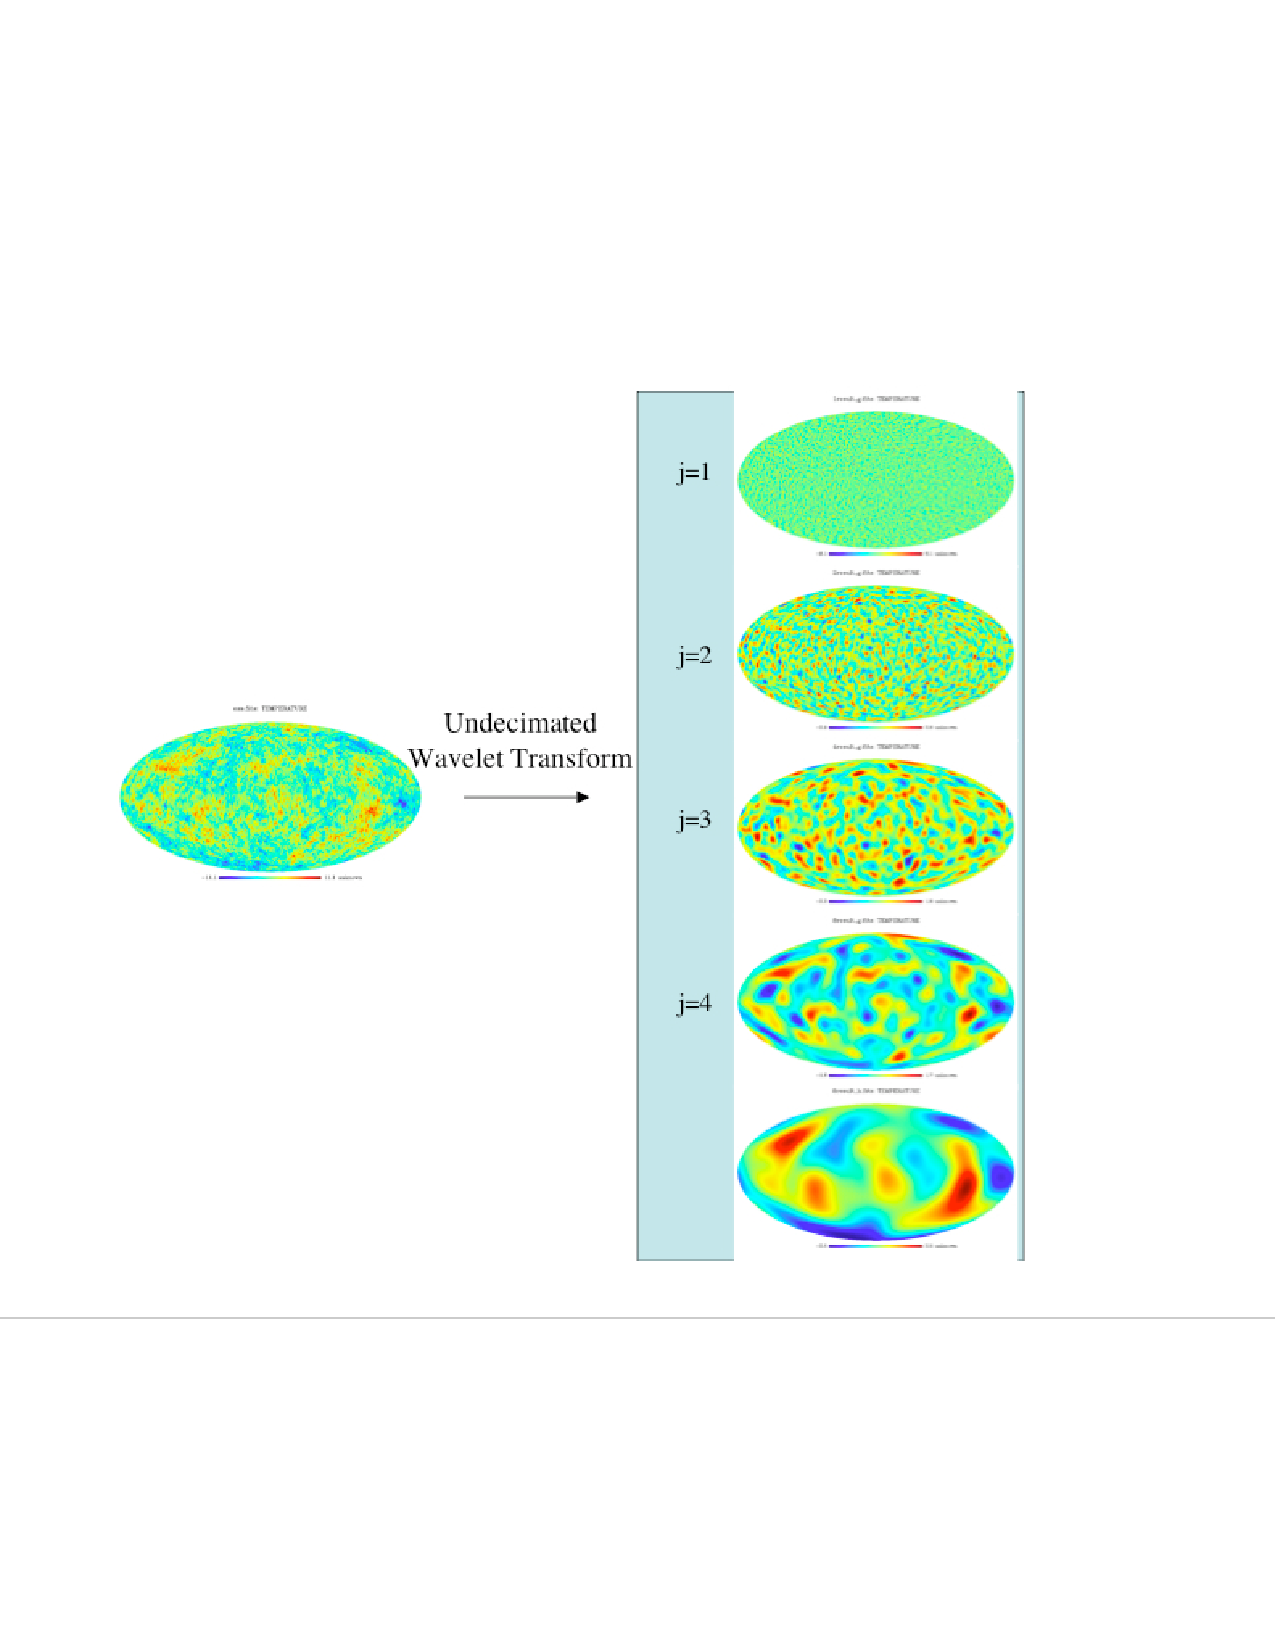
\includegraphics[height=8truecm,width=6truecm]{fig_uwt_sphere.pdf}
% 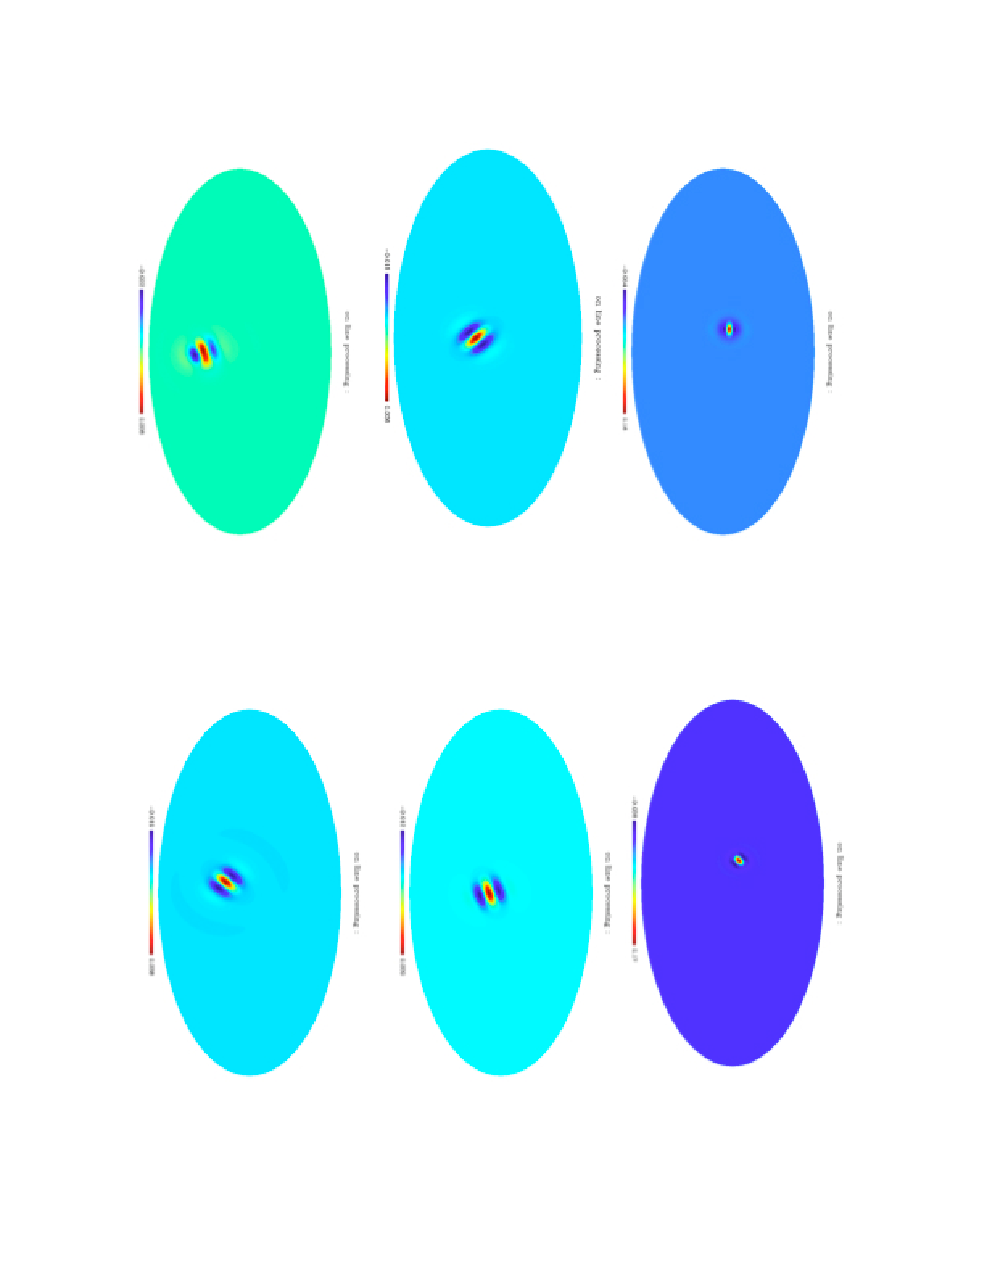
\includegraphics[height = 5 in]{fig_back_cur_sphere.pdf}
\centerline{
\hbox{
\psfig{figure=fig_cbf5_synchrotron_bw.pdf,bbllx=0.5cm,bblly=9.5cm,bburx=20cm,bbury=20cm,width=8cm,height=4.5cm,clip=}
\psfig{figure=fig_resi_cbf5_synchrotron_bw.pdf,bbllx=0.5cm,bblly=9.5cm,bburx=20cm,bbury=20cm,width=8cm,height=4.5cm,clip=}
}}
\caption{Denoising. Combined Filtering Method (pyramidal wavelet and pyramidal curvelet) and residual.}
\label{Figure:sync_cbf_filter}
\end{figure}


\begin{figure}
\centerline{
\hbox{
% \psfig{figure=fig_result_cbf_face5_bw.ps,bbllx=1.5cm,bblly=4.5cm,bburx=20cm,bbury=23cm,height=10cm,width=10cm,clip=}
\psfig{figure=fig_cmp_fil_synchrotron_face6_bw.pdf,bbllx=1.5cm,bblly=12.5cm,bburx=10.5cm,bbury=25.5cm,height=19.5cm,width=13.5cm,clip=}
}}
\caption{{ Combined Filtering Method, face 6 in the Healpix representation of the image shown in figure~\ref{Figure:sync_cbf_filter}. 
From top to bottom and left to right, respectively the a) original image face, b) the noisy image, c) the combined filtered image, 
d) the combined filtering residual, e) the wavelet filtering residual and f) the curvelet filtering residual.}}
\label{Figure:sync_face_cbf_filter}
\end{figure}

Although the results obtained by simply thresholding the curvelet expansion are encouraging, there is of course ample room for further
improvement. A quick inspection of the residual images for both the wavelet and curvelet transforms shown in Figure~\ref{Figure:sync_filter}
reveals the existence of very different features. For instance, wavelets do not restore long features with high fidelity while curvelets
are seriously challenged by isotropic or small features. Each transform has its own area of expertise and this complementarity is of great 
potential. The Combined Filtering Method (CFM) \cite{starck:spie01a} allows us to benefit from the advantages of both transforms. This iterative 
method detects the significant coefficients in both the wavelet domain and the curvelet domain and guarantees that the reconstructed map will 
take into account any pattern which is detected as significant by either of the transforms. A full description of the algorithm is given in Appendix B.
Figure~\ref{Figure:sync_cbf_filter} shows the CFM denoised image and its residual. { Figure~\ref{Figure:sync_face_cbf_filter} shows one face 
(face 6) of the following Healpix images: upper left, original image; upper right, noisy image; middle left, restored image after denoising 
by the combined transform; middle right, the residual; bottom left and right, the residual using respectively the curvelet and the wavelet 
denoising method. } The results are reported in Table~\ref{comptab_sync}. The residual is much better when the combined filtering is applied, 
and no feature can be detected any more by eye in the residual. This was not the case for either the wavelet and the curvelet filtering.

% \section{Deconvolution ?}
  
\chapter{Sparse Component Analysis, data restoration and inpainting on the sphere}
\label{ch_sca_datarest}

\section{Morphological Component Analysis on the sphere}

A usual task  in processing signals, images as well as spherical data maps, is to decompose the data 
into its elementary building blocks. This can be formulated as an inverse problem where the data is 
assumed to have been generated according to the following model : 
\begin{equation}
 y = \sum_{i} \alpha_i \phi_i + \eta
\end{equation}
that is a linear combination of relevant waveforms $\phi_i \in \mathbb{R}^n$ with weights $\alpha_i$. 
Here $\eta$ represents possible contamination by additive, typically Gaussian white noise. Given data 
$y\in \mathbb{R}^n$, one then wants to recover the underlying structures that is to say estimate a set 
of waveforms $\phi_i$ that build the data and their corresponding weights $\tilde{\alpha}_i$. The solution 
to this estimation problem will depend heavily on the available prior information. Of interest here is 
the case where one is given \emph{a priori} a set a waveforms from which to select a good subset. This set 
may be a basis, a frame or several bases or frames grouped into a large redundant dictionary.\\
%
Possible dictionaries in 1D and 2D include Fourier and related bases, wavelet bases, as well as 
other more recent multiscale systems such as the ridgelet~\cite{cur:candes99_1} and curvelet 
frames~\cite{cur:donoho99,starck:sta01_3}, etc. Depending on the morphology of the data, each of 
these dictionaries will have different performance characteristics 
%perform more or less efficiently 
in a non-linear approximation scheme. For instance, sparse approximations of piecewise smooth 
signals or images with point singularities are easily obtained using wavelets. However these 
are no longer optimal in the case of piecewise smooth images with singularities along smooth 
curves or edges. Such images are more efficiently approximated using curvelets which are highly 
anisotropic and thus exhibit high directional selectivity. Digital implementations of both ridgelet 
and curvelet transforms and their application to image denoising are described in~\cite{starck:sta01_3}.\\
%
Available transforms in the spherical topology include the spherical harmonics and several 
wavelet transforms. Software packages such as Healpix\footnote {http://www.eso.org/science/healpix}~\cite{pixel:healpix} 
or Glesp~\cite{pixel:glesp} provide approximate digital spherical harmonic transform routines 
based on their specific pixelization schemes. Schr{\"o}der and Sweldens~\cite{wave:sweldens95a} 
have developed an orthogonal wavelet transform on the sphere based on the Haar wavelet function 
which then suffers from the poor frequency domain localization properties of the primitive Haar function 
%properties of the Haar function 
and from the problems inherent in orthogonal decomposition (\emph{e.g.} lack of translation invariance). 
A few papers describe continuous wavelet transforms on the sphere~\cite{wave:antoine99bis,wave:cayon01,wave:holschneider96,wave:wiaux,bogdanova} 
which have been extended to directional wavelet transforms~\cite{wave:wiaux2005,wave:hobson04}. 
Although useful for data analysis, these continuous transforms lack an inverse transform and hence 
are clearly not suitable for restoration or synthesis purposes.\\
%
In their pioneering  work, Freeden and Maier~\cite{freeden02,freeden03} gave a wavelet transform 
and reconstruction scheme on the sphere which is based on the spherical harmonic transform. 
Following this idea, Starck \emph{et al.}~\cite{starck:sta05_2} have proposed a new invertible 
isotropic undecimated wavelet transform (UWT) on the sphere which preserves the same desirable 
properties as the standard isotropic UWT for flat 2D maps~\cite{starck:book98}: the reconstruction 
is simple and immediate since it is just the addition of all the wavelet bands with the coarsest scale. 
Based on this new decomposition, other multiscale transforms such as the pyramidal wavelet transform, 
the ridgelet transform and the curvelet transform have been successfully constructed on the sphere \cite{starck:sta05_2}. 
%
Each of these decompositions on the sphere will sparsely represent parts of the image based 
on their morphological properties. Wavelets will easily detect more or less isotropic localized 
structures, while curvelets are better suited for efficiently detecting highly anisotropic objects.\\
%
% ,  based on the spherical harmonics decomposition, is to our knowledge the only one to have an inverse transform. This set of spherical transforms has recently been enriched with a new invertible  isotropic undecimated wavelet transform~\cite{starck:sta05_2} the properties of which are similar to those of the \emph{\`a trous} algorithm and with digital ridgelet and curvelet transforms on the sphere. These tools make it possible to detect both point singularities and  edges in spherical maps. 
%
%
A data set $y$ has an exact representation over any complete basis of the data space, or several 
such exact representations in the case of redundant overcomplete dictionaries. However, these 
representations are not equally interesting in terms of data modeling or feature detection. In fact, 
a strong \emph{a priori} is to favor representations of $y$ that use only a small number of waveforms 
leading to a more concise and possibly more interpretable representation of the data. In fact, 
building sparse representations or approximations is the (he)art of structured data processing: 
the design of good detection, denoising, restoration and compression algorithms relies on the 
availability of good dictionaries and good selection algorithms. Indeed, selecting the smallest 
subset of waveforms from a large dictionary, that will linearly combine to reproduce the salient 
features of a given signal or image, is a hard combinatorial problem. Several \emph{pursuit} algorithms 
have been proposed that can help build very sparse decompositions such as the greedy Matching Pursuit (MP)~\cite{wave:mallat93} 
algorithm which refines the signal approximation by picking at each iteration the one waveform 
which best correlates with the current approximation error. Basis Pursuit (BP) ~\cite{wave:donoho98} 
is a global procedure which seeks an approximation $\tilde{y}$ to $y$ by solving the linear programming problem:
\begin{equation}
\min_{ \alpha } ~ \|\alpha\|_{{ \ell_1}} \mbox{ subject to } y = \Phi \alpha.
\label{eqn_bp}
\end{equation}
where the ${\ell_1}$ norm measures sparsity in place of the ${\ell_0}$ counting norm. 
%
In the presence of noise, a noise-aware variant of BP, known as BPDN (for BP denoising), can be 
stated as a convex quadratic programming problem and solved using the Interior Point method 
\cite{wave:donoho98}. The BPDN problem can also be written in the augmented Lagrangian form:
\begin{equation}
\min_{ \alpha } ~  \|y - \Phi\alpha\|_{{ \ell_2}} ^2 + \lambda \cdot \|\alpha\|_{ \ell_1}
\label{eqn_mp}
\end{equation}
Among all possible solutions, the chosen one has the minimum ${\ell_1}$ norm. This choice of 
$\ell_1$ norm is very important. An $\ell_2$ norm, as used in the method of frames \cite{wave:daube88b}, 
does not favor sparsity \cite{wave:donoho98}. A number of recent results prove that these 
algorithms will recover the unique maximally sparse decomposition provided this solution is 
sparse enough and the dictionnary is sufficiently incoherent~\cite{Donoho-Elad,cur:elad02,miki:Gribonval-Nielsen,miki:Temlyakov,miki:fuchs}. 
Nevertheless, in problems involving large data sets~(\emph{e.g.} images, spherical maps), 
BP or MP synthesis algorithms are computationally prohibitive.
%
Morphological Component Analysis (MCA) is a recent faster alternative described in~\cite{starck:sta04} 
%\cite{starck:elad05,starck:sta04_1,starck:sta04,SPIE2005a} 
that  constructs a sparse representation of a signal or an image assuming that it is a combination 
of morphologically distinct features which are sparsely represented in different dictionaries 
associated with fast transform algorithms. For instance, images commonly combine contours and textures: 
the former are well accounted for using curvelets, while the latter may be well represented using 
local cosine functions. In searching for a sparse decomposition of a signal or image $y$, it is 
assumed that $y$ is a sum of $K$ components $ (s_k)_{1,\ldots,K}$, where each can be described as 
$s_k = {\bf \Phi}_k \alpha_k$ with a possibly over-complete dictionary ${\bf \Phi}_k$ and a sparse 
vector of coefficients $\alpha_k$. It is further assumed that for any given component the sparsest 
decomposition over the proper dictionary yields a highly sparse description, while its decomposition 
over the other dictionaries, ${\bf \Phi}_{k'\ne k}$, is non sparse. Thus, the different ${\bf \Phi}_k$ 
can be seen as discriminating between the different components of the initial signal. MCA achieves its 
sparse decomposition relying on an iterative thresholding algorithm with a successively decreasing 
threshold~\cite{starck:bobin06_tip} thus refining the current approximation by including finer structures 
alternatingly in the different morphological components. Based on MCA, it has also been shown that we can 
derive a very efficient inpainting method \cite{starck:elad05}.\\
%
{\em This paper: } Motivated by the success of MCA in signal and image processing, the purpose of this contribution 
is to take advantage of the variety of transforms on the sphere recently made available~\cite{starck:sta05_2} to extend 
the applicability of MCA to the analysis of spherical maps which are commonly recorded in a number of areas such as 
geophysics, astrophysics or medical imaging. As in the case of Euclidean 2D images, we further extend the MCA algorithm 
on the sphere in order to perform inpainting tasks on the sphere. The proposed numerical tools are shown to be valuable 
in several selected applications in physics and astrophysics. The construction of the undecimated isotropic wavelet and 
curvelet transforms on the sphere is reviewed in the next section. Sections~\ref{sect_mca} and~\ref{sect_inpaint} describe 
the extension to the sphere of the MCA algorithm and of its modification for inpainting purposes. 


\section{MCA on the Sphere}
\label{sect_mca}
%---------------------------------------------------------------------------------------------------------------------------------------
%---------------------------------------------------------------------------------------------------------------------------------------
%a short introduction to this section?
%%---------------------------------------------------------------------------------------------------------------------------------------
%	\subsection{Introduction}
%%---------------------------------------------------------------------------------------------------------------------------------------
%---------------------------------------------------------------------------------------------------------------------------------------
 \subsection{Principle and algorithm}
 %---------------------------------------------------------------------------------------------------------------------------------------
For a given spherical map $y$ modeled as a linear { combination} of $K$ spherical maps $s_k$, $y = \sum_{k=1}^K s_k$, 
having different morphologies, MCA assumes that a dictionary of bases $\{ {\bf \Phi}_1,\cdots,{\bf \Phi}_K\}$ exists 
such that, for each $ ~ k$, $ s_k$ is sparse in $ ~ {\bf \Phi}_k$ while its representation in the other 
$ ~ {\bf \Phi}_{k'}$ ($ ~ k' \ne k$) is not sparse : $ ~ \forall k' \neq k, ||{\bf \Phi}_k^T s_k||_0 < ||{\bf \Phi}_{k'}^T s_k||_0$, 
where $||x||_0$ denotes the $\ell_0$ pseudo-norm of the vector $x$
%  (\textit{i.e.}  the number of non-zero coefficients of $x$)
The problem is to separate the mixture $y$ into its constitutive morphological components $ (s_k)_{k=1,\cdots,K}$ relying 
on the discriminating power of the different dictionaries ${\bf \Phi}_k$. Ideally, the $\alpha_k$ are the solutions { to} :
\begin{equation}\label{eq:Separation1}
 ~ 
\min_{ {\alpha}_1, \dots, ~{\alpha}_K }~\sum_{k=1}^K\|{\alpha}_k\|_0 \quad \mbox{subject to } \quad y= \sum_{k=1}^K  {\bf \Phi}_k {\alpha}_k
\end{equation}
While sensible from the point of view of the desired solution, the problem formulated in Equation (\ref{eq:Separation1}) 
is non-convex and combinatorial by nature. Its complexity grows exponentially with the number of columns in the overall 
dictionary { (NP-hard problem)}. Motivated by recent equivalence results \emph{e.g.} in~\cite{Donoho-Elad}, the MCA 
algorithm seeks a solution to the following minimization problem: 
\begin{equation}\label{mca:model1}
 ~ 
\min_{s_1,\ldots,s_K} \lambda \sum_{k=1}^K  \|\alpha_k\|_1 + \left\|y-\sum_{k=1}^K s_k\right\|_2^2\,\,\,\textrm{with}\,\,\,s_k ={\bf \Phi}_k \alpha_k 
\end{equation}
where an ${ \ell_1}$ sparsity measure is substituted to the $\ell_0$ counting norm following a prescription of 
the Basis Pursuit algorithm \cite{wave:donoho98}. In the above, the equality constraint was relaxed and again 
$ ~ s_k = {\bf \Phi}_k \alpha_k $. In the case where each ${\bf \Phi}_k$ is an orthonormal basis, 
{ a block-coordinate solution to the above problem is given by} the following set of coupled equations:
\begin{equation}
 ~
\forall k, s_k = r_k - \frac{\lambda_k}{2 }  {\bf \Phi}_k  \mbox{sign}( {\bf \Phi}_k^{T} s_k ) \mbox{  with  } r_k = s - \sum_{k' \neq k} s_{k'}
\end{equation}
This can be solved efficiently using the iterative \textit{Block-Coordinate Relaxation Method} \cite{text:Bruce98} 
in conjunction with, at a given $k$, a soft-thresholding of the decomposition of $r_k$ over ${\bf {\bf \Phi}_k}$. 
However, when non-unitary or redundant transforms are used, the above is no longer strictly valid. Nevertheless, 
simple shrinkage still gives satisfactory results as explained in~\cite{miki:shrinkage}. Finally, denoting by 
${\bf T}_k$ and ${\bf R}_k$ the forward and inverse transforms associated with the redundant dictionary 
${\bf {\bf \Phi}_k}$, MCA seeks a solution to problem~(\ref{mca:model1}) with the following algorithm: 
\begin{center}
\begin{minipage}[b]{0.9\linewidth}
\vspace{0.1in}
\footnotesize{\textsf{1. Set the number of iterations $I_{\max}$ and the initial thresholds $ ~ \left(\lambda_k^{(0)}\right)_{k}$}

\textsf{2. While  $\lambda^{(t)}_{k}$ is greater than a given lower bound $\lambda_{\min}$ (e.g. can depend on the noise standard deviation), }

\hspace{0.15in} \textsf{-- Proceed with the following iteration to estimate components $ (s_k)_{k=1,\ldots,K}$ at iteration $t$:}

\hspace{0.25in} \textsf{For $ ~ k=1,\cdots,K$ }

\hspace{0.5in} \textsf{$\bullet$ Compute the residual term $ ~ r_k^{(t)}$ assuming the current estimates $\tilde{s}_{k' \neq k}^{(t-1)}$ of $ ~ s_{k' \neq k}$, are 
fixed:}

\hspace{0.75in} \textsf{ $ ~ r_k^{(t)} = y - \sum_{k' \neq k} \tilde{s}_{k'}^{(t-1)}$}

\hspace{0.5in} \textsf{$\bullet$ Estimate the current coefficients of $ ~ \tilde{s}_k^{(t)}$ by thresholding with threshold $ ~ \lambda_k^{(t)}$:}

\hspace{0.75in} \textsf{$ \tilde{\alpha}_k^{(t)} = \delta_{\lambda_k^{(t)}}\left( {\bf T}_k r_k^{(t)}\right)$}

\hspace{0.5in} \textsf{$\bullet$ Get the new estimate of $ s_k$ by reconstructing from the selected coeffcients $ \tilde{\alpha}_k^{(t)}$ :}

\hspace{0.75in} \textsf{$ ~ \tilde{s}_k^{(t)} = {\bf R}_k \tilde{\alpha}_k^{(t)}$}

\hspace{0.15in} \textsf{-- Decrease the thresholds $\lambda_{k}$ following a given strategy.}
}
\vspace{0.05in}
\end{minipage}
\end{center}
%---------------------------------------------------------------------------------------------------------------------------------------
	\subsection{Thresholding strategy}
%---------------------------------------------------------------------------------------------------------------------------------------
The operator $\delta$ in the above algorithm is a soft thresholding operator as a result of the use of an 
${ \ell_1}$ sparsity measure in approximation to the ideal $ ~ \ell_0$ norm. In practice, hard thresholding 
leads generally to better results~\cite{starck:sta04}. The final threshold should vanish in the { noiseless} 
case or it may be set to a multiple of the noise standard deviation in the presence of noise as in common 
detection or denoising methods. The way the threshold is decreased along the iterations of the proposed 
iterative thresholding scheme is paramount in terms of performance of the MCA separation mechanism. 
The original algorithm~\cite{starck:sta04} used a linear strategy :  
\begin{equation}
\lambda^{(t)} = \lambda^{(0)} - (t-1)\frac{\lambda^{(0)} -\lambda_{\min}}{I_{\max}-1}
\end{equation}
where $\lambda^{(0)}$ is the initial threshold, and $I_{\max}$ is the number of iterations. The first threshold 
can be set automatically to a large enough value such as the maximum of all coefficients { $\lambda^{(0)}=\max_k~\|{\bf T}_k y\|_\infty$}. 
But there is no way to estimate the minimum number of iterations yielding a successful separation. Too small a number 
of iterations leads to bad separation while too large a number is computationally costly. Further, experiments have 
clearly shown that the optimal number of iterations depends on the data. We recently focused on devising some new data 
adaptive thresholding strategies to speed up the MCA decomposition preserving the quality of the component separation. 
Hereafter we describe two promising strategies, namely MAD and MOM, in the case where $K = 2$ ; 
generalizing to $K\geq2$ is straightforward.
%~\cite{starck:bobin06_tip,starck:dave06}.
\paragraph{MAD} Consider a map $y$ such that $ ~ y = s_1 + s_2 = {\bf \Phi}_1\alpha_1 + {\bf \Phi}_2\alpha_2$ 
where $ ~ s_1$ and $ ~ s_2$ have similar ${ \ell_2}$ norm and $ \alpha_{k=1,2} = {\bf \Phi}_{k=1,2}^T s_{k=1,2}$ are sparse. 
When both $ ~ {\bf \Phi}_{k=1,2}$ are orthonormal bases, decomposing $y$ in ${\bf \Phi}_{1}$ leads to 
$ y {\bf \Phi}_{1}^T = \alpha_1 + {\bf \Phi}_1^T{\bf \Phi}_2\alpha_2 $. Provided the mutual coherence~\cite{Elad-Bruckstein,miki:Gribonval-Nielsen,Donoho-Elad} 
of ${\bf \Phi}_1$ and ${\bf \Phi}_2$ is low, $y_2$ has no particular structure in ${\bf \Phi}_{1}$ and hence 
it is tempting to model $ ~ {\bf \Phi}_1^Ts_2$ as a Gaussian \emph{noise}. Its { standard deviation} can be 
estimated using a robust estimator such as the Median Absolute Deviation (MAD)~\cite{rest:donoho93_1}. It follows that 
estimating the significant entries $\tilde{\alpha_1}$ in $\alpha_1$ is a denoising problem readily solved 
by thresholding ${\bf \Phi}_{1}^T y$ with { a} threshold $k\sigma$ { (typically $k$ is in the range 3 to 4)}. 
The next step is to project the residual $ ~†y - \tilde{s_1} = y - {\bf \Phi}_{1}\tilde{\alpha_1}$ on ${\bf \Phi}_2$ and so on. 
Clearly, the variance of the residual decreases along iterations and so this provides a simple strategy to adaptively 
control the threshold in the MCA algorithm. In practice, this strategy remains fruitful in the case of redundant dictionaries. 
Donoho \emph{et al.} in \cite{starck:dave06} have recently focused on an iterative thresholding scheme applied to solving 
under-determined linear sparse problems in which they use a similar rule to manage their decreasing threshold.
%
\paragraph{MOM}  Let $ ~ \tilde{s}_1^{(t)}$ and $ ~ \tilde{s}_2^{(t)}$ denote the current estimates of 
components $ ~ s_1$ and $ ~ s_2$ at the $t^{th}$ iteration of the MCA decomposition of $y$. The current 
residual is $ ~ r^{(t)} = y -  \tilde{s}_1^{(t)} - \tilde{s}_2^{(t)} $. In the strategy coined MOM as in 
"Mean of Max", the value of the threshold at iteration $ ~ t$ is given by : 
\begin{equation}
\label{MOM_threshold}
 ~ 
\lambda^{(t)} = \frac{1}{2}\left[ ||{\bf \Phi}_1^T\left( y- \tilde{s}_1^{(t-1)} - \tilde{s}_2^{(t-1)} \right)||_\infty + ||{\bf \Phi}_2^T\left( y- \tilde{s}_1^{(t-1)} - \tilde{s}_2^{(t-1)} \right)||_\infty\right]
\end{equation}
which is easily computed at each step of the iterative process. When one considers more than two dictionaries, 
one should take the mean of the two largest decomposition coefficients of the full residual over two distinct dictionaries. 
The intuition underlying this strategy is that the next significant coefficients to be selected should be attached 
to the dictionary in which the projection of the full residual has coefficients of largest amplitudes. Assuming the 
coefficients selected at iteration $ ~ t$ are in ${\bf \Phi}_1$, it can be shown, under some conditions on the sparsity 
of the components and the mutual coherence of the dictionary~\cite{starck:bobin06_tip}, that the proposed strategy 
fixes the threshold so that :
\begin{equation}
\label{intuitive_choice}
||{\bf \Phi}_1^T{\bf \Phi}_2\bar{\alpha}_2^{(t-1)} ||_\infty < \lambda_1^{(t)} < ||\bar{\alpha}_1^{(t-1)} ||_\infty, \bar{\alpha}_{k=1,2}^{(t-1)}=\alpha_{k=1,2}-\tilde{\alpha}_{k=1,2}^{(t-1)}
\end{equation}
hence avoiding false detections (upper bound) and ensuring that at least one coefficient is selected (lower bound). 
This thresholding strategy can easily be made more or less conservative depending on the desired decomposition speed. 
With these new thresholding strategies, MCA is a fast and robust algorithm to achieve sparse decompositions in redundant 
dictionaries and a practical alternative to other well-known sparse decomposition algorithms~\cite{starck:bobin06_tip}. 
\subsection*{Example}
\begin{figure}
\vbox{
\centerline{
\hbox{
%\psfig{figure=test_gauss_alm_bw.ps,bbllx=0.cm,bblly=6.5cm,bburx=22.cm,bbury=21.5cm,height=6.5cm,width=8cm,clip=}
\psfig{figure=test_gauss_alm_bw.ps,bbllx=0.cm,bblly=8.5cm,bburx=22.cm,bbury=19.5cm,height=4cm,width=6.5cm,clip=}
}
}
\centerline{
\hbox{
%\psfig{figure=test_gauss_alm_mca_alm_bw.ps,bbllx=0.cm,bblly=8.5cm,bburx=22cm,bbury=19.5cm,height=4.5cm,width=8cm,clip=}
%\psfig{figure=test_gauss_alm_mca_wt_bw.ps,bbllx=0.cm,bblly=8.5cm,bburx=22cm,bbury=19.5cm,height=4.5cm,width=8cm,clip=}
\psfig{figure=test_gauss_alm_mca_alm_bw.ps,bbllx=0.cm,bblly=8.5cm,bburx=22cm,bbury=19.5cm,height=4cm,width=6.5cm,clip=}
\psfig{figure=test_gauss_alm_mca_wt_bw.ps,bbllx=0.cm,bblly=8.5cm,bburx=22cm,bbury=19.5cm,height=4cm,width=6.5cm,clip=}
}
}
}
\caption{ Simple toy experiment with MCA on the sphere - The top map shows a linear combination of a spherical harmonic function and a localized Gaussian-like function on the sphere. The bottom maps show the resulting separated components that were obtained using the proposed Morphological Component Analysis on the sphere.}
\label{Figure:mcatoy}
\end{figure}
The spherical maps shown on { figure~\ref{Figure:mcatoy}} illustrate a simple numerical experiment. 
We applied the proposed Morphological Component Analysis on the Sphere to synthetic data resulting 
from the linear mixture of components respectively sparse in the spherical harmonics and the isotropic 
wavelet representations. The method was able to separate the data back into its original constituents. 
A more involved application is described in the next section.    
%---------------------------------------------------------------------------------------------------------------------------------------
\subsection{Application in Physics}
\label{section:bedros}
In Inertial Confinement Fusion (ICF) a spherical shell is irradiated by laser energy directly or after the 
laser energy has been converted to soft X-rays~\cite{bedros:atzeni}. Either way, the aim is to implode the 
capsule which contains a shell of nuclear fusion fuel (deuterium and tritium) ready to ignite if, after it 
has been imploded, its density is high enough and a hot spot in its center becomes hot enough to cause a 
propagating nuclear burn wave to travel through the rest of the fuel. This ultimate energy source will not 
work if during the implosion hydrodynamic instabilities develop which can break apart the shell before it 
assembles at the center and a hot spot forms~\cite{bedros:lindl}. Hydrodynamic instabilities such as Rayleigh-Taylor 
occur due to nonuniformities in the laser spatial profile or imperfections in the composition of multiple 
surfaces which make up the layers of thin material that surround the nuclear  fuel. Very small amplitude imperfections 
initially can result in the ultimate failure of the target due to the large compression ratios involved in ICF.
\begin{figure}
\centerline{
\hbox{
\psfig{figure=bed_mca_orig_data.ps,bbllx=1.5cm,bblly=10cm,bburx=19cm,bbury=19.cm,height=4cm,width=6.5cm,clip=}
\psfig{figure=bed_mca_large_scale.ps,bbllx=1.5cm,bblly=10cm,bburx=19cm,bbury=19.cm,height=4cm,width=6.5cm,clip=}
}
}
\caption{ \textbf{left : }Surface structures of ICF spherical shells measured on the nanometer scale are a superposition of global scale variations, isolated bumps and scratches as well as artifacts which look like interference patterns on intermediate scales. \textbf{right :} Coarsest scale of the undecimated isotropic wavelet transform of the surface measurements of an ICF target.}
\label{bedros_mca_data}
\end{figure}
It is therefore extremely important to characterize the inner and outer surfaces of ICF shell targets 
so as to know whether they are worthy of consideration for ICF implosions. One day in a reactor setting 
tens of thousands of targets will have to be imploded daily so that checking each one is totally 
out of the question. Instead, very good target fabrication quality control processes have to be adopted so that 
confidence levels in proper performance will be high. A major step along this path to fusion energy then is to 
understand why imperfections occur and to correct the systematic elements and control the harm done by random sources.
%
Fine structures on the surfaces of spherical shells can be measured on the nanometer scale, among others, 
by atomic force microscopy or phase shifting spherical diffractive optical interferometry. An example of 
such measurements is shown on figure~\ref{bedros_mca_data}. As can be seen from the figure, there appears 
to be a superposition of global scale variations, isolated bumps and scratches as well as artifacts which 
look like interference patterns on intermediate scales of localization. The latter must be isolated and 
eliminated from consideration when deciding the readiness of the target for implosion. We have achieved 
the morphological feature separation by first doing an isotropic wavelet transform on the spherical data 
and subtracting the coarsest scale information. MCA on the sphere was used on the rest of the image using 
the undecimated wavelet and the local cosine transforms on the sphere. The isolated bumps were thus identified 
and the measurement technique caused artifacts were removed easily. The resulting bumps added to the coarsest scale, 
is the clean data with the interference patterns and artifacts removed as shown in figure~\ref{bedros_mca_result}. 
The spherical harmonic decomposition of the cleaned image gives rise to coefficients of various $\ell$ modes 
which will be amplified by the implosion process which can now be assessed correctly using numerical hydrodynamics 
simulation generated growth factors. If the bumps are clustered and not randomly distributed, then systematic errors 
in the manufacturing process can be tracked down. A code called MODEM has been put together to study such 
target surface data and extract the localized bump statistics including their correlations in height, 
size and relative location. For more details see~\cite{bedros:modem}.
\begin{figure}
\vbox{
\centerline{
\hbox{
\psfig{figure=bed_mca_in_data.ps,bbllx=1.5cm,bblly=10cm,bburx=19cm,bbury=19.cm,height=4cm,width=6.5cm,clip=}
}
}
\centerline{
\hbox{
\psfig{figure=bed_mca_out_dct.ps,bbllx=1.5cm,bblly=10cm,bburx=19cm,bbury=19.cm,height=4cm,width=6.5cm,clip=}
\psfig{figure=bed_mca_out_wt.ps,bbllx=1.5cm,bblly=10cm,bburx=19cm,bbury=19.cm,height=4cm,width=6.5cm,clip=}
}
}
}
\caption{\textbf{top :} Spherical map obtained by subtracting the coarse scale map on the right of figure~\ref{bedros_mca_data} from the initial map on the left of figure~\ref{bedros_mca_data}. \textbf{ bottom :} Component maps separated by the MCA method on the sphere : interference patterns and measurement artifacts were grabbed by the local cosine functions on the sphere (left) while  the isolated bumps were caught using the undecimated wavelet on the sphere (right). Adding back the coarse scale on the right of figure~\ref{bedros_mca_data} to the latter map results in a clean map of the surface structures of an ICF spherical shell with the interference patterns and artifacts removed.} 
\label{bedros_mca_result}
\end{figure}
%---------------------------------------------------------------------------------------------------------------------------------------
\section{Inpainting on the Sphere}
\label{sect_inpaint}
%---------------------------------------------------------------------------------------------------------------------------------------
\subsection{Algorithm}
%---------------------------------------------------------------------------------------------------------------------------------------
Named after the expert recovery process used for the restoration of deteriorated masterpieces, inpainting refers to a set 
of techniques used to alter images in a way that is undetectable to people who are unaware of the original images. There are 
numerous applications among which removing scratches or objects in digitized photographs, removing overlayed text or graphics, 
filling-in missing blocks in unreliably transmitted images, predicting values in images for better compression or image upsampling. 
Inpainting algorithms strive to interpolate through the gaps in the image relying on the available pixels, the continuation of edges, 
the periodicity of textures, etc. The preservation of edges and texture, in other words discontinuities, across gaps has attracted 
much interest, and many contributions have been proposed to solve this interpolation task. Non-texture image inpainting has received 
considerable interest and excitement since the pioneering paper by Masnou and Morel \cite{Masnou98, Masnou02} who proposed variational 
principles for image disocclusion. A recent wave of interest in inpainting has started from the recent contributions of Sapiro 
\emph{et al.}~\cite{text:sapiro1,text:sapiro2,text:sapiro3}, followed by Chan and Shen~\cite{text:chan1}. In these works, authors point 
to the importance of geometry and design anisotropic diffusion PDEs to fill in gaps by smooth continuation of isophotes. 
PDE methods have been shown to perform well on piecewise smooth functions.
% 
A very different approach is the inpainting algorithm based on MCA described in~\cite{starck:elad05} which has proved capable 
of filling in holes in either texture or cartoon content in 2D images. To make the link between building sparse representations 
and inpainting, consider the effect of a rectangular gap on the set of Fourier coefficients of a monochromatic sinewave : 
because of the non-locality of the Fourier basis functions it takes a large number of coefficients to account for the gap, 
which is known as the Gibbs effect. Seeking a sparse representation of the incomplete sine-wave outside the gap, that is without 
fitting the gap, enables the recovery of the complete monochromatic sinewave.
%
Following~\cite{starck:elad05}, an inpainting algorithm on the sphere is readily built from the Morphological Component Analysis 
on the sphere described in the previous section. Consider a discrete spherical data map $y$ and a binary map $M$ such that ones 
in $M$ indicate that the corresponding pixels in $y$ are valid data while zeros indicate invalid data. The objective function of 
MCA~(eq.~\ref{mca:model1}) can be modified as follows : 
 \begin{equation}\label{inp:model}
\min_{s_1,\ldots,s_n} \lambda \sum_{k=1}^K  \|\alpha_k\|_1 + \left\|M  \odot (y-\sum_{k=1}^K s_k) \right\|_2^2\,\,\,\textrm{with}\,\,\,s_k ={\bf \Phi}_k \alpha_k .
\end{equation}
where $\odot$ stands for entry-wise multiplication. Thus we are preventing the sparse model under construction from attempting to fit 
the invalid data. Other constraints can be easily imposed on the interpolated sparse components. For instance, in~\cite{starck:elad05}, 
a total variation penalty is shown to enhance the recovery of piece-wise smooth components. Asking for the regularity across the gaps of 
some localized statistics (~\emph{e.g.} enforcing that the empirical variance of a given inpainted sparse component be \emph{nearly equal} 
outside and inside the masked areas) are other possible constraints. In practice, because of the lack of accuracy of some digital 
transformations we used in the spherical topology, additional constraints, which may be relaxed close to convergence, were also found 
useful in some cases to stabilize the described iterative algorithms. 
%
It is proposed that a solution to the above minimization problem can be reached using the same iterative thresholding process as 
in the MCA algorithm detailed in the previous section, with the only required modification consisting in \emph{masking} the full 
residual using $M$ after each residual estimation. The MCA-inpainting algorithm is as follows : 
\begin{center}
\begin{minipage}[b]{0.9\linewidth}
\vspace{0.1in}
\footnotesize{\textsf{1. Set the number of iterations $I_{\max}$ and the initial thresholds $ \lambda^{(0)} $}

\textsf{2. While  $ ~†\lambda^{(t)}_{k}$ is greater than a given lower bound $\lambda_{\min}$ (e.g. can depend on the noise standard deviation), }

\hspace{0.15in} \textsf{-- Proceed with the following iteration to estimate components $ (s_k)_{k=1,\ldots,K}$ at iteration $t$:}

\hspace{0.25in} \textsf{For $ ~ k=1,\cdots,K$ }

\hspace{0.5in} \textsf{$\bullet$ Compute the residual term $  ~ r^{(t)}$ :}

\hspace{0.75in} \textsf{ $  ~ r^{(t)} = y - \sum_{k} \tilde{s}_{k}^{(t-1)}$}

\hspace{0.5in} \textsf{$\bullet$ Estimate the current coefficients of $  ~ \tilde{s}_k^{(t)}$ by thresholding with threshold $ ~ \lambda_k^{(t)}$:}

\hspace{0.75in} \textsf{$  \tilde{\alpha}_k^{(t)} = \delta_{\lambda_k^{(t)}}\left( {\bf T}_k \left(M \odot  r^{(t)}+\tilde{s}_k^{(t-1)}\right)\right)$}

\hspace{0.5in} \textsf{$\bullet$ Get the new estimate of $s_k$ by reconstructing from the selected coeffcients $  \tilde{\alpha}_k^{(t)}$ :}

\hspace{0.75in} \textsf{$  ~ \tilde{s}_k^{(t)} = {\bf R}_k \tilde{\alpha}_k^{(t)}$}

\hspace{0.15in} \textsf{-- Decrease the thresholds $\lambda_{k}$ following a given strategy.}
}
\vspace{0.05in}
\end{minipage}
\end{center} 
The different thresholding strategies described in the previous section can be used in the proposed MCA inpainting iterative thresholding algorithm. 
%
\subsection*{Example}
\begin{figure*}
\vbox{
\centerline{
\hbox{
\psfig{figure=earth_ori.ps,bbllx=0.cm,bblly=8.8cm,bburx=22cm,bbury=19.75cm,height=3.6cm,width=6.3cm,clip=}
\psfig{figure=earth_mask.ps,bbllx=0.cm,bblly=8.8cm,bburx=22cm,bbury=19.75cm,height=3.6cm,width=6.3cm,clip=}
}
}
\centerline{
\hbox{
\psfig{figure=earth_recons.ps,bbllx=0.cm,bblly=8.8cm,bburx=22cm,bbury=19.75cm,height=3.6cm,width=6.3cm,clip=}
\psfig{figure=earth_diff.ps,bbllx=0.cm,bblly=8.8cm,bburx=22cm,bbury=19.75cm,height=3.6cm,width=6.3cm,clip=}
}
}
}
\caption{ Application of the proposed MCA-inpainting algorithm on the sphere. \textbf{top left :} original satellite view of the Earth (~$mean= 76.9$, $\sigma =  47.7$~).  \textbf{top right :} incomplete map retaining 40 percent of the original pixels.  \textbf{bottom left : } inpainted map.  \textbf{bottom right :} map of reconstruction errors (~$mean= 0.0$, $\sigma =  2.86$ empirically estimated from the reconstructed pixels only~).}
\label{Figure:mcaearth}
\end{figure*}
A simple numerical experiment is shown on figure~\ref{Figure:mcaearth}. Starting with a full satellite view 
of the Earth\footnote{availbale from : http://www.nasa.gov/vision/earth/features/bmng\_gallery\_4.html}, 
an incomplete spherical map was obtained by randomly masking some of the pixels. In fact, as much as sixty percent 
of the pixels were masked. Using both the spherical harmonics transform and the curvelet transform on the sphere 
within the proposed MCA inpainting algorithm, it is possible to fill in the missing pixels in a visually undetectable way. 
The residual map is shown at the bottom right of figure~\ref{Figure:mcaearth}. 
%---------------------------------------------------------------------------------------------------------------------------------------
\subsection{Application in Astrophysics}
%---------------------------------------------------------------------------------------------------------------------------------------
A major issue in modern cosmology is the measurement and the statistical characterization (spatial power spectrum, Gaussianity) 
of the slight fluctuations in the Cosmic Microwave Background radiation field. These are indeed strongly related to the cosmological 
scenarios describing the properties and evolution of our Universe. Some 370 000 years after the 'Big Bang', when the temperature 
of the Universe was around 3000~K, thermal energy was no longer sufficient to keep electrons and positively charged particles apart 
so they combined. Photons were then set free in a nearly transparent Universe. Since the Universe further expanded, these photons 
are now in the microwave range but they should still be distributed according to a Black Body emission law. Indeed, before recombination, 
the Universe was a highly homogeneous opaque plasma in near thermal equilibrium in which photons and charged particles were highly interacting. 
Hence the slight fluctuations in matter density from which such large scale structures as galaxies or clusters of galaxies have evolved, 
are also imprinted on the distribution of photons. 
\begin{figure}
\vbox{
\centerline{
\hbox{
\psfig{figure=ima_wmap3y.ps,bbllx=1.5cm,bblly=10cm,bburx=19cm,bbury=19.cm,height=4cm,width=6.5cm,clip=}
\psfig{figure=wmap3y_inp.ps,bbllx=1.5cm,bblly=10cm,bburx=19cm,bbury=19.cm,height=4cm,width=6.5cm,clip=}
}
}
}
\caption{ \textbf{left :} CMB data map provided by the WMAP team. Areas of significant foreground contamination in the galactic region and at the locations of strong radio point sources have been masked out. \textbf{right :} Map obtained by applying the proposed MCA-inpainting algorithm on the sphere to the former incomplete WMAP CMB data map.}
\label{Figure:cmb_wmap_inpainting}
\end{figure}
The Cosmic Microwave Background~(CMB) was first observed in 1965 by Penzias and Wilson confirming a prediction 
made by Gamow in the late 1940's. But it was not until the early 1990's that evidence for small fluctuations 
in the CMB sky could finally be found thanks to the observations made by COBE~\cite{astro:COBE}. This was confirmed 
by several subsequent observations and recently by NASA's Wilkinson Microwave Anisotropie Probe\footnote{The WMAP data and mask we used here are available online at http://map.gsfc.nasa.gov/}. 
Full-sky multi-spectral observations with unprecedented sensitivity and angular resolution are expected from 
the ESA's PLANCK\footnote{http://astro.estec.esa.nl/Planck} mission, which is to be launched in 2008. The statistical 
analysis of this data set will help set tighter bounds on major cosmological parameters.
%
\begin{figure}
\vbox{
\centerline{
\hbox{
\psfig{figure=tpjls_mask_kp0.ps,bbllx=1.5cm,bblly=10cm,bburx=19cm,bbury=19.cm,height=4cm,width=6.5cm,clip=}
\psfig{figure=wt_wmap_inp_scale_1.ps,bbllx=1.5cm,bblly=10cm,bburx=19cm,bbury=19.cm,height=4cm,width=6.5cm,clip=}
}
}

\centerline{
\hbox{
\psfig{figure=wt_wmap_inp_scale_2.ps,bbllx=1.5cm,bblly=10cm,bburx=19cm,bbury=19.cm,height=4cm,width=6.5cm,clip=}
\psfig{figure=wt_wmap_inp_scale_3.ps,bbllx=1.5cm,bblly=10cm,bburx=19cm,bbury=19.cm,height=4cm,width=6.5cm,clip=}
}
}

\centerline{
\hbox{
\psfig{figure=wt_wmap_inp_scale_4.ps,bbllx=1.5cm,bblly=10cm,bburx=19cm,bbury=19.cm,height=4cm,width=6.5cm,clip=}
\psfig{figure=wt_wmap_inp_scale_5.ps,bbllx=1.5cm,bblly=10cm,bburx=19cm,bbury=19.cm,height=4cm,width=6.5cm,clip=}
}
}
\centerline{
\hbox{
\psfig{figure=wt_wmap_inp_scale_6.ps,bbllx=1.5cm,bblly=10cm,bburx=19cm,bbury=19.cm,height=4cm,width=6.5cm,clip=}
\psfig{figure=wt_wmap_inp_scale_7.ps,bbllx=1.5cm,bblly=10cm,bburx=19cm,bbury=19.cm,height=4cm,width=6.5cm,clip=}
}
}
}
\caption{ \textbf{left :} Mask provided by the WMAP team. The dark blue pixels indicate areas of high level foreground contamination in the WMAP CMB data map.  \textbf{From top to bottom and left to right :} Maps of the wavelet decomposition on seven scales of the inpainted WMAP CMB map shown on the right of figure~\ref{Figure:cmb_wmap_inpainting}. From the visual point of view, the masked area cannot be distinguished anymore in the wavelet scales of the inpainted map.}
\label{Figure:cmb_scale_wmap_inpainting}
\end{figure}
There are nonetheless a few practical issues and notably that several other astrophysical sources also emit radiation 
in the frequency range used for CMB observations~\cite{fb-rg99}. Separating back the observed mixtures into maps of 
the different astrophysical contributions in order to isolate the CMB properly is a difficult inverse problem for which 
methods and algorithms are being actively designed (see \emph{e.g.}~\cite{astro:2005MNRAS.364.1185P,starck:bobin06,starck:yassir05,wlens:pires06} 
and references therein). The estimated spherical CMB maps will inevitably be contaminated by some level of residual 
contributions, most significantly in the galactic region and at the locations of strong radio point sources. Therefore, it is 
common practice to mask out that part of the data (\emph{e.g.} using the mask shown on figure~\ref{Figure:cmb_scale_wmap_inpainting} 
upper left, provided by the WMAP team) in order to reliably assess the non-gaussianity of the CMB field through estimated 
higher order statistics (\emph{e.g.} skewness, kurtosis ) in various representations (\emph{e.g. wavelet, curvelet, etc.}) 
\cite{starck:sta03_1,starck:jin05}. But the gaps in the data thus created need to be handled properly as the detection 
of non-gaussianity in CMB would have a major scientific impact. The proposed MCA-inpainting on the sphere was used here 
successfully to fill in the masked regions in order to restore the stationarity of the observed CMB field and lower the impact 
of the incompleteness of the data set on the estimated measures of non-gaussianity or any other non-local statistical test. 
The experiment was conducted on several simulations of full-sky Gaussian CMB maps. A typical CMB map (the CMB data map disclosed 
by the WMAP consortium) is shown on figure~\ref{Figure:cmb_wmap_inpainting} along with the map obtained as a result of 
the inpainting process allowing for a first visual assessment of the quality of the proposed method. Figure~\ref{Figure:cmb_scale_wmap_inpainting} 
shows the wavelet decomposition of the inpainted map. We can see that the mask is not visible at all in the different scales. 
Here we have applied the MCA-Inpainting algorithm with 200 iterations and a single transform which was the Spherical 
Harmonic Decomposition. A more quantitative evaluation of the proposed inpainting algorithm is reported on figure ~\ref{Figure:mca_skew_kur} 
where plots of the estimated measures of non-Gaussianity on both the original map and the inpainted map are given. 
These reveal no significant discrepancy: we believe that the proposed method will help discriminate between truly non-Gaussian CMB 
and non-Gaussianity related to the non-stationarity of incomplete maps. This will be further investigated in the future.
\begin{figure}
\vbox{
\centerline{
\hbox{
\psfig{figure=skewness.ps,bbllx=1cm,bblly=1cm,bburx=17cm,bbury=14cm,height=4.5cm,width=6.5cm,clip=}
\psfig{figure=kurtosis.ps,bbllx=1cm,bblly=1cm,bburx=17cm,bbury=14cm,height=4.5cm,width=6.5cm,clip=}
}
}
}
\caption{ Horizontally is the scale number increasing for lower frequencies. \textbf{Left :} skewness of the wavelet coefficients in a given scale of the original complete simulated spherical CMB map ($\times$) and of the inpainted map ($\lozenge $). \textbf{Right :} kurtosis of the wavelet coefficients in a given scale of the original complete simulated spherical CMB map ($\times$) and of the inpainted map ($\lozenge $). Error bars were estimated on a small set of fifteen simulated complete CMB maps.}
\label{Figure:mca_skew_kur}
\end{figure}


\section{Generalized Morphological Component Analysis on the sphere}

\label{sec:gmca}
\subsection{The GMCA model}
\label{sec:model}

The observation with detector $i$ is then a noisy linear mixture of $n$ independent sources $\{s_j\}_{j=1,\cdots,n}$ : 
$x_i = \sum_{j=1}^n a_{ij} s_j + n_i$. The coefficient $a_{ij}$ reflects the emission law of source $s_j$ in the 
frequency band of the $i$-th sensor; $n_i$ models instrumental noise. When $m$ sensors provide observations at 
different frequencies, this linear mixture model can be rewritten in a more convenient matrix formulation :
\begin{equation}
\label{eq:lm_model}
{\bf X} = {\bf AS} + {\bf N}
\end{equation}
where ${\bf X}$ is the $m \times t$ data matrix the rows of which are the observed data maps in each channel, ${\bf A}$ 
is the $m \times n$ mixing matrix, ${\bf S}$ is the $n \times t$ source matrix the rows of which are the sources $s_j$, 
and ${\bf N}$ is the $m \times t$ noise matrix.

We further assume that all the protagonists of the model in Equation~\ref{eq:lm_model} are random components (variables 
or vectors). More particularly, the entries of the noise matrix ${\bf N}$ are assumed to be \textit{independently} 
distributed according to a zero mean Gaussian distribution with variance $\sigma_i^2$ depending on the detector. 
From physical considerations, ${\bf N}$ models instrumental noise the level of which varies independently from one 
detector to another. ${\bf N}$ is thus a random Gaussian variable with zero mean and covariance matrix 
${\bf \Gamma_N} = \mbox{diag}(\sigma_1^2,\cdots,\sigma_m^2)$. In practice, as the detectors are assumed to be accurately calibrated, 
${\bf \Gamma_N}$ is known with high precision. The log-likelihood function is then the following one :
\begin{equation}
\label{eq:ll}
\log P({\bf X} \big| {\bf A},{\bf S},{\bf \Gamma_N}) = -\frac{1}{2} \|{\bf X} - {\bf AS}\|_{2,{\bf \Gamma_N}}^2 + C
\end{equation}
where $C$ is a constant. The notation $\| . \|_{2,{\bf \Gamma_N}}^2$ stands for the Frobenius norm of ${\bf Y}$ in the noise 
covariance metric : $\| Y \|_{2,{\bf \Gamma_N}}^2 = \mbox{ Trace}\left( {\bf Y}^T {\bf \Gamma_N}^{-1} {\bf Y}\right)$. 
From a Bayesian point of view, adding physical priors should help the separation task. We first assume no particular knowledge 
about the emission laws of the components modeled by ${\bf A}$. For simplicity, we consider that each entry of the mixing 
matrix ${\bf A}$ is \textit{i.i.d.}\footnote{Independently and identically distributed.} from a uniform zero mean distribution. 
Note that it would be possible to add some physical constraint on the emission laws reflected in ${\bf A}$.

In the general case, source separation is merely a question of diversity and contrast between the sources (see \cite{Cardo1}). 
For instance, on the one hand JADE relies on non-gaussianity to distinguish between the sources. On the other, SMICA takes advantage 
of the diversity of the mixed components' power spectra to achieve the separation task. ``Non-gaussianity" and ``power spectra diversity" 
are contrasts between the sources. A combination of both characteristics, ``Non-gaussianity" and ``power spectra diversity", 
was also proposed to separate CMB from kinetic SZ signal which are otherwise undistinguishable \cite{forni}. Recent work has 
already emphasized on sparsity as a source of diversity to improve component separation (see \cite{Zibu} and \cite{MMCA}). 
In that setting, each source $\{s_j\}_{j=1,\cdots,n}$ is assumed to be sparse in a representation (potentially overcomplete) $\mathcal{D}$. 
Formally, $\mathcal{D}$ is a fixed dictionary of signal waveforms written as a $T \times t$ matrix. We define the set of projection 
coefficients $\alpha_j$ such that : $\forall j \in \{1,\cdots,n\}, \quad s_j = \alpha_j \mathcal{D}$. Any source $s_j$ is said 
to be sparse in $\mathcal{D}$ if most of the entries of $\alpha_j$ are nearly zero and only a few have ``significant" amplitudes. 
When $\mathcal{D}$ is overcomplete ($T > t$), $\mathcal{D}$ is called a dictionary. Overcomplete representations attractiveness 
in image processing theory leans on their potential to generate very sparse representations of data based on their morphological 
content (see e.g. \cite{DH} and references therein).

In the field of basic source separation we showed in \cite{MMCA} that morphological diversity and sparsity are key properties 
leading to better separation. We noticed that the gist of sparsity-based source separation methods leans on the rationale : 
``\textit{independent sources are distinctly sparse in a dictionary $\mathcal{D}$}". In that study, we considered the simple 
case of morphologically different sources : components were assumed to be sparsely represented in different sub-dictionaries. 
We illustrated that such sparsity prior provides a very effective way to distinguish between sources. In the present paper, 
we focus on a more general setting : the sources can have similar morphologies (\textit{i.e.} all the sources are sparsely 
represented over the whole $\mathcal{D}$). When the overcomplete dictionary $\mathcal{D}$ is made of the union of $D$ orthonormal 
bases (\textit{i.e.} $\mathcal{D} = \left[\Phi_1,\cdots,\Phi_D\right]$) then each source is modeled as the linear combination 
of $D$ so-called morphological components (see \cite{SED} for details on Morphological Component Analysis) - each morphological 
component being sparse in a different orthonormal basis $\{\Phi_1,\cdots,\Phi_D\}$:
\begin{eqnarray}
\forall  j\in \{1,\cdots,n\}, \quad s_j  & = &  \sum_{k=1}^D \varphi_{jk} = \sum_{k=1}^D \alpha_{jk} \Phi_k
\end{eqnarray}
From a statistical viewpoint, we assume that the entries of $\alpha_{jk} = \varphi_{jk}\Phi_k^T$ are \textit{i.i.d} from 
a Laplacian probability distribution with scale parameter $1/\mu$:
\begin{equation}
\label{eq:source_prior}
P(\varphi_{jk}) \propto \exp\left(- \mu \|\varphi_{jk}\Phi_k^T\|_1\right)
\end{equation}
where the $\ell_1$-norm $\|.\|_1$ stands for $\|x\|_1 = \sum_{p=1}^t |x[p]|$ in which $x[p]$ is the $p$-th entry of $x$. In practice, 
the Laplacian prior is well adapted to model leptokurtic sparse signals. We classically assume that the morphological components are 
statistically mutually independent : $P({\bf S}) = \prod_{j,k} P(\varphi_{jk})$. Estimating the sources ${\bf S}$ is then equivalent 
to estimating the set of morphological components $\{\varphi_{jk}\}_{j=1,\cdots,n;k=1,\cdots,D}$. In this Bayesian context, we propose 
to estimate those morphological components $\{\varphi_{jk}\}$ and the mixing matrix ${\bf A}$ from a \textit{maximum a posteriori} (MAP) 
leading to the following optimization problem:
\begin{equation}
\left\{\{\hat{\varphi}_{jk}\},{\bf \hat{A}}\right\} = {\arg\max}_{\{\varphi_{jk}\},{\bf A}} P({\bf X}|{\bf A},\{\varphi_{jk}\},{\bf \Gamma_N}) \prod_{j,k}P(\varphi_{jk}) P({\bf A})
\end{equation}
where we further assumed that the morphological components $\{\varphi_{jk}\}$ are independent of ${\bf A}$. Owing to Equations~\ref{eq:ll} 
and \ref{eq:source_prior}, the mixing matrix ${\bf A}$ and the morphological components $\{\varphi_{jk}\}$ are obtained by minimizing 
the following negative log \textit{a posteriori}:
\begin{equation}
\label{eq:optim}
\left\{\{\hat{\varphi}_{jk}\},{\bf \hat{A}}\right\} = {\arg\min}_{\{\varphi_{jk}\},{\bf A}}\|{\bf X} - {\bf AS}\|_{2,{\bf \Gamma_N}}^2 + 2 \mu \sum_{j=1}^n \sum_{k=1}^D \|\varphi_{jk}\Phi_k^T\|_1
\end{equation}
where $\forall j \in \{1,\cdots,n\},\quad s_j = \sum_{k=1}^D \varphi_{jk}$. Equation~\ref{eq:optim} leads to the GMCA estimates 
of the sources and the mixing matrix in a general sparse component separation context. Interestingly, in the case of CMB data, 
the sources we look for (CMB, galactic dust and SZ) are quite sparse in the same unique orthonormal wavelet basis. The dictionary
$\mathcal{D}$ then reduces to a single orthonormal basis $\Phi$. In that case, since $\Phi$ is unitary, Equation~\ref{eq:optim} 
can be rewritten as follows :
\begin{eqnarray}
\label{eq:foptim}
\left\{{\bf \hat{\alpha}},{\bf \hat{A}}\right\} &=& {\arg\min}_{{\boldsymbol \alpha},{\bf A}} \|{\bf X}\Phi^T - {\bf A\alpha}\|_{2,{\bf \Gamma_N}}^2 + 2 \mu \|{\boldsymbol \alpha}\|_1 \nonumber \\
						&=& {\arg\min}_{{\boldsymbol \alpha},{\bf A}} f_\mu({\boldsymbol \alpha},{\bf A}) = {\arg\min}_{{\boldsymbol \alpha},{\bf A}} f_0({\bf A}, {\boldsymbol \alpha}) + 2\mu f_1({\boldsymbol \alpha})
\end{eqnarray}
where ${\boldsymbol \alpha} = {\bf S}\Phi^T$. Note that the estimation is done in the sparse representation $\Phi$ requiring a single 
transform of the data ${\bf X}\Phi^T$. To remain computationally efficient, GMCA relies on practical transforms which generally involve 
fast implicit operators (typical complexity of $\mathcal{O}\left(t\right)$ or $\mathcal{O}\left(t \log t \right)$). In \cite{Zibu}, 
the authors also used a unique orthonormal wavelet basis. While a gradient descent is used in \cite{Zibu}, we use a fast and efficient 
iterative thresholding optimization scheme which we describe in the next section.

\subsection{Solving the optimization problem}
\label{sec:algo}
The \textit{maximum a posteriori} estimates of the coefficients ${\boldsymbol \alpha}$ and the mixing matrix in Equation~\ref{eq:foptim} 
lead to a non-convex minimization problem. Note that in Equation~\ref{eq:foptim} the functional to be minimized suffers from several 
invariances : any permutation or rescaling of the sources and the mixing matrix leaves the product $\bf A{\boldsymbol \alpha}$ unaltered. 
The scale invariance is computationally alleviated by forcing the columns of ${\bf A}$ to have unit $\ell_2$ norm~: $\forall i\in{1,\cdots,n},\quad a^{i^T}a^i = 1$ 
where $a^i$ is the $i$-th column of ${\bf A}$. 

As solutions of problem~(\ref{eq:foptim}) have no explicit formulation, we propose solving it by means of a block-coordinate relaxation 
iterative algorithm such that each iteration $(h)$ is decomposed into two steps : (i) estimation of the sources ${\bf S}$ assuming the 
mixing matrix is fixed to its current estimate ${\bf \hat{A}}^{(h-1)}$ and (ii) estimation of the mixing matrix assuming the sources are 
fixed to their current estimates ${\bf \hat{S}}^{(h)}$. It is not difficult to see that the objective MAP functional in (\ref{eq:foptim}) 
is continuous on its effective domain and has compact level sets. Moreover, this objective function is convex in the source coefficient 
vectors $(\alpha_1,\ldots,\alpha_n)$, and $f_0$ has an open domain, is continuous and G\^ateaux differentiable. Thus by \cite[Theorem 4.1]{Tseng2001}, 
the iterates generated by our alternating algorithm are defined and bounded, and each accumulation point is a stationary point of the MAP 
functional. In other words, our iterative algorithm will converge. Hence, at iteration $(h)$, the sources are estimated from a \textit{maximum a posteriori} 
assuming ${\bf A} = {\bf \hat{A}}^{(h-1)}$. By classical ideas in convex analysis, a necessary condition for ${\boldsymbol \alpha}$ to be 
a minimizer is that the zero is an element of the subdifferential of the objective at ${\boldsymbol \alpha}$. We calculate\footnote{For clarity, 
we drop the upper script $(h-1)$ and write $\hat{\bf A} = \hat{\bf A}^{(h-1)}$.}:
\begin{equation}
\label{eq:subdiff}
\partial_{\boldsymbol \alpha} f_\mu({\boldsymbol \alpha},{\bf A})= -2{\bf {\bf A}}^T{\bf \Gamma_N}^{-1}({\bf X}\Phi^T - {\bf A}{\boldsymbol \alpha}) + 2\mu \partial_{\boldsymbol \alpha} \|{\boldsymbol \alpha}\|_1
\end{equation}
where $\partial_{\boldsymbol \alpha} \|{\boldsymbol \alpha}\|_1$ is defined as (owing to the separability of the prior):
\[
\partial_{\boldsymbol \alpha} \|{\boldsymbol \alpha}\|_1 = \left\{U \in \mathbb{R}^{n \times t} \Bigg| 
\begin{array}{ccc}
U{j,k} & = \mbox{ sign}(\alpha_{j,k}), & ~ \alpha_{j,k} \neq 0 \\
U{j,k} & \in [-1,1], & ~ \alpha_{j,k} = 0
\end{array} \right\}.
\]
Hence, Equation \ref{eq:subdiff} can be rewritten equivalently as two conditions leading to the following (proximal) fixed point equation:
\begin{equation}
\label{eq:it_estim1}
\begin{array}{cc}
\hat{\alpha}_{j,k} = 0, & \text{if} ~ \left|{\left({\bf A}^T{\bf \Gamma_N}^{-1}{\bf X}\Phi^T\right)}_{j,k} \right| \leq \mu \\
{\bf {\bf A}}^T{\bf \Gamma_N}^{-1}({\bf X}\Phi^T - {\bf A}\hat{\boldsymbol \alpha}) = \mu \mbox{ sign}\left(\hat{\boldsymbol \alpha}\right), & \text{otherwise}. 
\end{array}
\end{equation}
Unfortunately, Equation~\ref{eq:it_estim1} has no closed-form solution in general. It must be iterated and is thus computationally demanding. 
Fortunately, it can be simplified when ${\bf A}$ has nearly orthogonal columns in the noise covariance matrix (\textit{i.e.} 
${\bf \hat{A}}^T{\bf \Gamma_N}^{-1}{\bf \hat{A}} \simeq \mbox{diag}\left({\bf \hat{A}}^T{\bf \Gamma_N}^{-1}{\bf \hat{A}}\right)$). 
Let ${\bf C} = {\left({\bf \hat{A}}^T{\bf \Gamma_N}^{-1}{\bf \hat{A}}\right)}^{-1}{\bf A}^T{\bf \Gamma_N}^{-1}{\bf X}\Phi^T$, Equation~\ref{eq:it_estim1} 
boils down to the following set of equations $\forall j\in\{1,\cdots,n\}$:
\begin{equation}
\label{eq:it_estim}
\begin{array}{ccc}
\hat{\alpha}_{j,k} & = 0, \quad \text{if} ~ \left|{{\bf C}}_{j,k} \right| \leq \mu^{(h)} \sigma_j^2 \\
\hat{\alpha}_j & = {\left[{\bf C}\right]}_j - \mu \sigma_j^2  \mbox{ sign}\left(\hat{\alpha}_j\right), \quad \text{otherwise}.
\end{array}
\end{equation}
where $[{\bf Y}]_j$ is the $j$-th row of ${\bf Y}$. In practice, even if the approximation we make is not strictly valid, such a simplification 
leads to good computational results. These equations are known as soft-thresholding with threshold $\mu^{(h)} \sigma_j^2$. We define $\mathrm{ST}_{\delta}(.)$, 
the soft-thresholding operator with threshold $\delta$. At iteration $(h)$, the sources are thus estimated such that:
\begin{equation}
\hat{\alpha}_j^{(h)} = \mathrm{ST}_{\mu^{(h)} \sigma_j^2}\left(\left[{\bf C}\right]_j\right)
\end{equation}
The $j$th source is reconstructed as $\hat{s}_j^{(h)} = \hat{\alpha}_j^{(h)}\Phi$. The mixing matrix ${\bf A}$ is then estimated by a maximum 
likelihood estimate amounting to a simple least-squares update assuming ${\bf S}$ is fixed. The GMCA algorithm is then described as follows :
\begin{flushleft}
\vspace{0.15in}
\centering
\begin{tabular}{|c|} \hline
\begin{minipage}[h]{0.95\linewidth}
\vspace{0.025in} \footnotesize{\textsf{1. Set the number of iterations $I_{\max}$ and thresholds $\delta_j^{(0)} = \mu^{(0)}\sigma_j^2$\\} 
\textsf{2. While each $\mu^{(h)}$ is higher than a given lower bound $\mu_{min}$ (e.g. can depend on the noise variance), \\}
\hspace{0.1in} \textsf{-- Proceed with the following iteration to estimate source coefficients ${\boldsymbol \alpha}$ at iteration $h$ assuming ${\bf A}$ is fixed:}
\hspace{0.2in} \textsf{$\hat{\alpha}_j^{(h)} = \mathrm{ST}_{\mu^{(h)} \sigma_j^2}\left(\left[{\left({\bf \hat{A}}^T{\bf \Gamma_N}^{-1}{\bf \hat{A}}\right)}^{-1}{\bf \hat{A}}^T{\bf \Gamma_N}^{-1}{\bf X}\Phi^T\right]_j\right)$:\\}
\hspace{0.1in} \textsf{-- Update $\bf A$ assuming ${\boldsymbol \alpha}$ is fixed :}
\hspace{0.2in} \textsf{${\bf \hat{A}}^{(h)} = {\bf X}\Phi^T{\bf \hat{\boldsymbol \alpha}}^T\left({\bf \hat{\boldsymbol \alpha}}{\bf \hat{\boldsymbol \alpha}}^T\right)^{-1}$\\}
\textsf{-- Decrease the threshold $\mu^{(h)}$ following a given strategy}}
\vspace{0.05in}
\end{minipage}
\\\hline
\end{tabular}
\vspace{0.15in}
\end{flushleft}
Note that the overall optimization scheme is based on an iterative and alternate thresholding algorithm involving a 
\textit{coarse to fine} estimation process. Indeed, \textit{coarse} versions of the sources (\textit{i.e.} containing 
the most ``significant" features of the sources) are first computed with high values of $\mu^{(h)}$.
%\begin{equation}
%\forall j\in\{1,\cdots,n\},\quad \hat{s}_j = \mathrm{ST}_{\mu^{(h)} \sigma_j^2}\left({\left({\bf \hat{A}}^T{\bf \Gamma_N}^{-1}{\bf \hat{A}}\right)}^{-1}{\bf \hat{A}}^T{\bf \Gamma_N}^{-1}{\bf X}\Phi^T\right)\Phi
%\end{equation}
In the early stages of the algorithm, the mixing matrix is then estimated from the most ``significant" features of the sources 
which are less perturbed by noise. The estimation of ${\bf A}$ and ${\bf S}$ is then refined at each iteration as $\mu^{(h)}$ 
(and thus the thresholds $\{\mu^{(h)}\sigma_j^2\}_{j=1,\cdots,n}$) decreases towards a final value $\mu_{min}$. We already used 
this minimization scheme in \cite{MMCA} where this optimization process provided robustness and helped convergence even in a 
noisy context. Experiments in Section~\ref{sec:results} illustrate that it achieves good results with GMCA as well.




\chapter{Blind Source Separation on the Sphere}
\label{ch_mrs_ica}

\section{Introduction}
\index{blind source separation}
\index{ICA}

Blind Source Separation (BSS) is a problem that occurs in multi-dimensional data processing. The overall goal is to recover 
unobserved signals, images or sources $S$ from mixtures of these sources $X$ observed typically at the output of an 
array of sensors. The simplest mixture model takes the form:
\begin{equation}\label{model0}
X = A S
\end{equation}
where $X$ and $S$ are random vectors of respective sizes $m \times 1$, $n \times 1$ and $A$ is an $m \times n$ matrix. The 
entries of $S$ are assumed to be independent random variables. Multiplying $S$ by $A$ linearly mixes the $n$ sources into 
$m$ observed processes. \\ 
   
Independent Component Analysis methods were developed to solve the BSS problem, i.e. given a batch of $T$ observed 
samples of $X$, estimate the mixing matrix $A$ and reconstruct the corresponding $T$ samples of the source vector $S$, relying 
mostly on the statistical independence of the source processes. Note that with the above model, the independent sources can 
only be recovered up to a multiplication by a non-mixing matrix i.e. up to a permutation and a scaling of the 
entries of $S$. Although independence is a strong assumption, it is in many cases physically plausible. The point is that 
it goes beyond the simple second order decorrelation obtained for instance using Principal Component Analysis (PCA) : decorrelation 
is not enough to recover the source processes since any rotation of a white random vector remains a white random vector.\\

Algorithms for blind component separation and mixing matrix estimation depend on the model used for the probability distribution 
of the sources. In a first set of techniques, source separation is achieved in a noise-less setting, based on the 
non-Gaussianity of all but possibly one of the components. Most mainstream Independent Component Analysis (ICA)  techniques belong to this category : JADE~\citep{ica:jade}, 
FastICA, Infomax~\citep{ica:icabook}. In a second set of blind techniques, the components are modeled as Gaussian processes, either 
stationary or non stationary and, in a given representation, separation requires that the sources have diverse, i.e. non 
proportional, variance profiles. The Spectral Matching ICA method (SMICA) ~\citep{ica:Del2003}, considers in this sense the case of 
mixed stationary Gaussian components and goes further than the above model Eq.~\eqref{model0} by taking into account additive 
instrumental noise $N$:
\begin{equation}\label{model1}
X = A S + N
\end{equation}
Moving to a Fourier representation, the idea is that colored components can be separated based on the diversity of their power spectra.\\ 
 
The next  section give a short overview of two significant ICA methods mentioned above and implemented in the \mrs package: 
JADE  and FastICA ~\citep{ica:icabook}. 
This is followed by a description of ways to 
combine wavelets and ICA techniques. Some useful properties of wavelet transforms can indeed come enhance the performance of ICA  methods in several situations. 
Finally, we present the method GMCA, which performs a blind source separation using the the sparsity concept.
    
\section{JADE}
\index{ICA!jade}

The Joint Approximate Diagonalization of Eigenmatrices method (JADE) assumes the observed data $X$ follows the noiseless mixture 
model~\eqref{model0} where the independent sources $S$ are non-Gaussian i.i.d.\footnote{The letters i.i.d. stand for 
independently and identically distributed meaning that each entries of $X$ at a given time $t$ are independent of $X$ at any other 
time $t'$ and that the distribution of $X$ does not depend on time.} random processes. The mixing matrix is assumed to be square 
and invertible so that (de)mixing is actually just a change of basis.

As mentioned above, second order statistics do not retain enough information for source separation in this context: finding a change of 
basis in which the data covariance matrix is diagonal will not in general enable to identify the independent sources properly. Nevertheless, 
decorrelation is half the job~\citep{ica:tutorial} and one may seek the basis in which the data is represented by maximally independent 
processes among those bases in which the data is decorrelated. This leads to so-called orthogonal algorithms: after a proper whitening of 
the data by multiplication with the inverse of a square root of the covariance matrix of the data $W$, one is then seeking a rotation $R$ 
(which leaves things white) so that $\hat{ S}$ defined by
\begin{equation}
\hat{ S} = W^{-1} \, Y =  W^{-1}\, R \, X_{\textrm{white}}  = W^{-1}\, R \, W \, X 
\end{equation}
and $\hat{B} = \widehat{A^{-1}} =  W^{-1}\, R \, W$ are estimations of the sources and of the inverse of the mixing matrix.\\

JADE is such an orthogonal ICA method and, like most mainstream ICA techniques, it exploits higher order statistics so as to achieve some 
sort of non linear decorrelation. Precisely, in the case of JADE, statistical independence is assessed using fourth order cross cumulants : 
%\begin{eqnarray} \nonumber	 
%F_{ijkl} & = & \textrm{cum}( y_i, y_j, y_k, y_l ) \nonumber \\
%  & = & \mathcal{E} (y_i y_j y_k y_l) - \mathcal{E} (y_i y_j)\mathcal{E} (y_k y_l) \nonumber \\
%  & & -\mathcal{E} (y_iy_l)\mathcal{E} ( y_j y_k)-\mathcal{E} (y_iy_k)\mathcal{E} (y_j y_k)
%\end{eqnarray}
\begin{eqnarray} \nonumber
F_{ijkl} & = & \textrm{cum}( y_i, y_j, y_k, y_l ) \nonumber \\
 & = & \mathcal{E} (y_i y_j y_k y_l) - \mathcal{E} (y_i y_j)\mathcal{E} (y_k y_l) -\mathcal{E} (y_iy_l)\mathcal{E} ( y_j y_k)-\mathcal{E} (y_iy_k)\mathcal{E} (y_j y_k)
\end{eqnarray}
where $\mathcal{E}$ stands for statistical expectation and the $y_i$'s are the entries of vector $Y$ modeled as random variables, 
and the correct change of basis (i.e. rotation) is found by somehow diagonalizing the fourth order cumulant tensor. 
Indeed, if the $y_i$'s were independent, all the cumulants with at least two different indices would be zero. As a consequence of 
the independence assumption of the source processes $S$ and of the whiteness of $Y$ for all rotations $R$, the fourth order 
tensor $F$ is well structured: JADE was precisely devised to take advantage of the algebraic properties of $F$. JADE's objective 
function is given by
\begin{eqnarray}  \nonumber	 
%\mathcal{J}_{\textrm{jade}}( R )   &=& \sum _{ijkl \ne ijkk}  \textrm{cum}(  y_i, y_j, y_k, y_l )^2  \nonumber    \\
  \mathcal{J}_{\textrm{jade}}( R ) & =&  \sum _{ij}   \sum_{k \ne l} \textrm{cum}(  y_i, y_j, y_k, y_l )^2  
\end{eqnarray}
which can be interpreted as a joint diagonalization criterion. Fast and robust algorithms are available for the minimization 
of $\mathcal{J}_{\textrm{jade}}( R )$ with respect to $R$ based on Jacobi's method for matrix diagonalization~\citep{ica:pham2001}. 
More details on JADE can be found in~\citep{ica:jade,ica:tutorial,ica:icabook}.


\subsubsection{JADE for spherical maps}

Applying JADE on multichannel data mapped to the sphere does not require any particular modification of the algorithm. Indeed, JADE estimates 
the fourth order cumulant tensor from the available data samples assuming an i.i.d. random field. Hence, given a pixelization scheme on 
the sphere such as provided by the Healpix package, JADE can be directly applied to the multichannel spherical data pixels.


\section{FastICA}
\index{ICA!fastica}

FastICA is by now a standard technique in ICA. Like JADE, it is meant for the analysis of mixtures of independent non-Gaussian sources in 
a noise-less setting. A complete description of this method can be found in \citep{ica:icabook} and references therein\footnote{Many papers on this 
algorithm are available at http://www.cs.helsinki.fi/u/ahyvarin/papers/fastica.shtml}. We give here a brief and simplified account 
of the algorithm. FastICA, again like JADE, is a so-called orthogonal ICA method: the independent components are sought by maximizing a 
measure of non-Gaussianity under the constraint that they are decorrelated. Intuitively, one should understand that mixtures of independent 
non-Gaussian random variables tend to look more Gaussian. An enlightening view on the relation between mutual information, which is 
a natural measure of independence, decorrelation and non-Gaussianity can be found in~\citep{ica:3easy,ica:geomindep}. Non-Gaussianity is assessed 
in FastICA using a contrast function $G$ based on a non-linear approximation to negentropy~\citep{ica:icabook}. In practice, depending 
on the application, different approximations or non-linear (non-quadratic) functions should be experimented with. In a simple deflation scheme, 
for sphered data, the directions are found sequentially : a direction $r$ of maximal non-Gaussianity is sought by maximizing
\begin{equation}
J_G(r) = \Big( \mathcal{E} \{ G(r^T x_{\textrm{white}}  ) \} - \mathcal{E} \{ G(\nu ) \} \Big)^2 
\end{equation}
where $\nu$ stands for centered unit variance Gaussian variable, under the constraint that $r$ has unit norm and that $r$ is orthogonal 
to the directions found previously.\\ \\
The contrast function $G$ can for instance be chosen among the following~\citep{ica:icabook}:
\begin{eqnarray}
G_0 (u)  & = &  \frac{1}{a} \textrm{log}\,\textrm{cosh} (a u ) \nonumber    \\
G_1 (u)  & = &  -\frac{1}{a} \textrm{exp}(- a u^2 / 2 )   \nonumber	   \\
G_2 (u)  & = &  \frac{1}{4} u^4 \nonumber    \\
\end{eqnarray}
where $a$ is a constant to be determined depending on the application. It can be shown that the maxima of $J_G$ occur at certain maxima 
of $\mathcal{E} \{ G(r^T x_{\textrm{white}} ) \} $. These are obtained for $r$ solution to :
\begin{equation}
\mathcal{E} \{ x_{\textrm{white}} g(r^T x_{\textrm{white}}  ) \} - \lambda r = 0 
\end{equation}
where $\lambda$ is a constant easily expressed in terms of the optimal direction $r_0$, and $g$ is the derivative of $G$. Solving this 
equation using Newton's method, and a few approximations, a fixed-point algorithm is derived which consists in repeating the 
following two steps until convergence :
\begin{eqnarray}
r  & \leftarrow & \mathcal{E} \{ x_{\textrm{white}} g(r^T x_{\textrm{white}}  ) \} - \mathcal{E} \{ g'(r^T x_{\textrm{white}}  ) \} r     \nonumber  \\
r  & \leftarrow  &  \frac{r}{\| r \|}   \nonumber	   \\
\end{eqnarray}
A simple implementation of this algorithm is included in the present package. It is largely based on the $\textbf{Matlab}^{TM}$ code 
available at www.cis.hut.fi/projects/ica/fastica/. 

 
\section{Wavelet and BSS} 
\index{wavelet!ICA}
\index{ICA!wavelet}

\label{sec:wjade}
\index{ICA!wjade}
\index{jade!wavelet}

Wavelets come into play as a sparsifying transform. Applying a wavelet transform on both sides of~\eqref{model0} does not affect the 
mixing matrix and the model structure is preserved. Also, moving the data to a wavelet representation does not affect its information 
content. However, the statistical distribution of the data coefficients in the new representation is different: wavelets are known to 
lead to sparse i.i.d. representations of structured data. Further, the local (coefficient wise) signal to noise ratio 
depends on the choice of a representation. A wavelet transform tends to grab the informative coherence between pixels while averaging 
the noise contributions, thus enhancing structures in the data. Although the standard ICA model~\eqref{model0} is for a noiseless setting, 
the derived methods can be applied to real data. Performance will depend on the detectability of significant coefficients i.e. on 
the sparsity of the statistical distribution of the coefficients. Moving to a wavelet representation will often lead to more robustness to noise.    

Once the data has been transformed to a proper representation (e.g. wavelets but also ridgelets and curvelets in the case of strongly 
anisotropic 2D or 3D data), WJADE (resp. WFastICA) consists in applying the standard JADE (resp. FastICA) method to the new multichannel coefficients. Once the mixing matrix 
is estimated, the initial source maps are obtained using the adequate inverse transform after some non linear denoising or thresholding of 
the coefficients if necessary.


\section{Sparse Blind Source Separation: the GMCA method}
% \section{Generalized Morphological Component Analysis on the sphere}
\label{sec:gmca}

\subsection{Morpho-Spectral Diversity}
%\label{sec:morph-spec-diversity}
Extending the redundant representation framework to the multichannel case requires defining what a multichannel overcomplete representation is.
Let us assume in this section that $\A = [\varphi_{\nu,1}, \cdots, \varphi_{\nu, N_c}] \in \RR^{N_c \times N_s}$ is a \textit{known spectral} dictionary, 
and $\W = [ \varphi_{1}, \cdots, \varphi_{T}] \in \RR^{N \times T}$ is a \textit{spatial} or \textit{temporal} dictionary\footnote{The adjectives 
\textit{spectral} and \textit{spatial} that characterize the dictionaries are not formal. Owing to the symmetry of the multichannel sparse decomposition problems, 
$\A$ and $\W$ have no formal difference. In practice and more particularly in multi/hyperspectral imaging, $\A$ will refer to the dictionary of physical spectra 
and $\W$ to the dictionary of image/signal waveforms. In the BSS problem, $\A$ is unknown.}. We assume that each source $s_i$ can be represented as 
a (sparse) linear combination of atoms in $\W$; $s_i=\W\alpha_i$. Let $\balpha$ the $N_s \times T$ matrix whose rows are $\alpha_i^\Tr$.

From Eq.~\eqref{model0}, the multichannel noiseless data $\bY$ can be written as
\be
\label{eq:tensor1}
\bY = \A\balpha\W^\Tr = \sum_{i=1}^{N_s}\sum_{j=1}^{T} \parenth{\varphi_{\nu,i}\varphi_{j}^\Tr}\alpha_i[j] ~.
\ee
Consequently, each column in of $\bY$ reads
\be
\label{eq:tensor2}
\bY[.,l] = \parenth{\A \otimes \W[l,.]} \mathrm{vect}(\balpha) ~, \quad \forall ~ l=1,\cdots,N ~,
\ee
and finally
\be
\label{eq:tensor3}
\mathrm{vect}(\bY) = \parenth{\A \otimes \W} \mathrm{vect}(\balpha) ~,
\ee
where $\otimes$ is the tensor (Kronecker) product and the operator $\mathrm{vect}$ stacks the columns of its argument in a long 1D vector. 
This latter equation brings a clear and simple insight: the sparsity of the sources in $\W$ translates into sparsity of the multichannel data 
$\bY$ in the multichannel tensor product dictionary ${\bf \Psi}=\A \otimes \W$. 

The multichannel dictionary $\bf \Psi$ can also be seen as concatenation of multichannel atoms ${\bf \Psi}^{(ij)}=\varphi_{\nu,i}\varphi_{j}^\Tr$ 
which are rank-one matrices obtained from each atomic spectrum $\varphi_{\nu,i}$ and each spatial elementary atom $\varphi_{j}$ (see Eq.~\eqref{eq:tensor1}). 

Some of the popular recovery results in sparse component analysis algorithm rely on the mutual coherence of 
the dictionary~\citep{cur:elad02,miki:Gribonval-Nielsen,mca:Donoho-Elad}. In the multichannel case a quantity 
of that kind can be defined. In fact, by standard properties of the tensor product, one can easily show that 
the Gram matrix of a tensor product is the tensor product of the Gram matrices. Thus the mutual coherence of the multichannel dictionary $\bf \Psi$ is:
\index{coherence}
\begin{equation}
\label{eq:mmc}
0 \le \mu_{\bf \Psi}  =  \max\left\{\mu_{\A},\mu_{\W}\right\} < 1 ~ .
\end{equation}

This expression of mutual coherence is instructive as it tells us that multichannel atoms can be distinguished 
based on their spatial or spectral morphology. In other words, discriminating two multichannel atoms $\Psi_{ij}$ and $\Psi_{i'j'}$ may put on different faces:
\begin{itemize}
\item{Spatial or temporal (respectively spectral) diversity:} in this case $i=i'$ and $j \neq j'$ (respectively $i \neq i'$ and $j = j'$). 
These atoms have the same spectrum (respectively, spatial shape) but one can discriminate between them based on their 
spatial (respectively, spectral) diversity. From \eqref{eq:mmc}, their coherence is lower than $\mu_{{\W}}$ (respectively $\mu_{{\A}}$). 
Disentangling these multichannel atoms can equivalently be done in \ref{ch_sca_datarest}.

\item{Both diversities:} $i \neq i'$ and $j \neq j'$, this seems to be a more favorable scenario to differentiate 
the atoms as they do not share neither the same spectrum nor the same spatial (or temporal) ``shape". Note that 
from \eqref{eq:mmc}, the coherence between these atoms in this case is lower than $\mu_{{\A}}\mu_{{\W}} \le \max\left\{\mu_{\A},\mu_{\W}\right\}$.
\end{itemize}

\subsection{Multichannel Sparse Decomposition}

We embark from Eq.~\eqref{eq:tensor1}, where the multichannel dictionary ${\bf \Psi}$ is supposed to be overcomplete, i.e. $NN_c < TN_s$. 
The goal is to recover the sparsest solution $\balpha$ from $\bY$ which requires solving:
\begin{equation}
\label{eq:multi_l0}
\min_{\balpha \in \RR^{N_s \times T}} \sum_{i=1}^{N_s}\norm{\alpha_i}_{0} \st \bY  = \A \balpha \W^\Tr.
\end{equation}
As justified in \ref{sect_mca}, this combinatorial problem can be replaced by its convex relaxation substituting the $\ell_1$ norm for the $\ell_0$ pseudo-norm, hence giving:
\begin{equation}
\label{eq:multi_l1}
\min_{\balpha \in \RR^{N_s \times T}} \sum_{i=1}^{N_s}\norm{\alpha_i}_{1} \st \bY  = \A \balpha \W^\Tr.
\end{equation}

As \eqref{eq:tensor3} is a vectorized monochannel form of \eqref{eq:tensor1}, what we are trying so do is actually to find 
the sparsest solution of a monochannel underdetermined system of linear equations where the solution is sparse in an 
overcomplete tensor product dictionary. Recovery properties of monochannel sparse decomposition by $\ell_1$ minimization 
were overviewed in chapter~\ref{ch_sca_datarest}. Therefore, if one is able to translate those identifiability criteria 
in the language of tensor product dictionaries, then we are done.

In particular, the coherence-based sparse recovery criterion given in \citep{DonohoHuo} is trivial to adapt owing to \eqref{eq:mmc}. 
Indeed, if $\bY$ is $k$-sparse in the multichannel dictionary ${\bf \Psi}$ with $k < C(\mu_{{\bf \Psi}}^{-1}+1)$ for some $C > 0$ (typically $C=1/2$), 
and the dictionary is sufficiently incoherent (both spectrally and spatially), then the solution of Eq.~\eqref{eq:multi_l1} is unique, 
is a point of equivalence of Eq.~\eqref{eq:multi_l0} and Eq.~\eqref{eq:multi_l1}, and the recovery is stable to bounded noise on $\bY$. 

Above, we addressed the multichannel sparse decomposition problem without assuming any constraint on the sparsity pattern 
of the different channels. It is worth however pointing out that sparse recovery conditions from multichannel measurements 
can be refined if some structured sparsity is hypothesized. For instance, for structured multichannel representation 
(e.g. sources with disjoint supports) \citep{GN05} provided coherence-based sufficient recovery conditions by solving Eq.~\eqref{eq:multi_l1}. 
One should note that despite apparent similarities, the multichannel sparse decomposition problem discussed here is conceptually 
different from the one targeting \textit{simultaneous} sparse recovery of multiple measurements vectors (MMV) considered by several authors, see e.g. 
\citep{CREK05,MalioutovMMV05,TroppMMV06,ChenHuo06,ArgyriouMMVLearning08,BachMMVLearning08,GribonvalMMV08,EldarMMV08,LouniciMMVLearning09,WainwrightMMV09}. 
The latter are not aware of any mixing process via $\A$, and their goal is to recover $\balpha$ from MMV $\bY=\balpha\W^\Tr$ in which 
the vectors $\alpha_i$, i.e. rows of $\balpha$, have a common sparsity pattern. However the MMV model can also be written 
$\mathrm{vect}(\bY^\Tr) = \parenth{\W \otimes \I} \mathrm{vect}(\balpha^\Tr)$ as in Eq.~\eqref{eq:tensor3}. The most widely used approach 
to solve the simultaneous sparse recovery problem with joint sparsity is to minimize a mixed $\ell_p-\ell_q$ norm of the form 
$\sum_{j=1}^T\parenth{\norm{\balpha[.,j]}_p^q}^{1/q}$ for $p \geq 1, 0 \leq q \leq +\infty$.

\subsection{Generalized Morphological Component Analysis}
\label{subsec:gmca}
We now turn to the BSS problem and highlight the role of sparsity and morphological diversity as a source of contrast to solve it. 
Towards this goal, we assume that the sources are sparse in the spatial dictionary $\W$ that is the concatenation of $K$ orthonormal bases 
$\parenth{{\W}_{k}}_{k=1,\cdots,K}$: $\W = \left[{\W}_{1},\cdots,{\W}_{K} \right]$. The restriction to orthonormal bases is only formal 
and the algorithms to be presented later still work in practice even with redundant sub-dictionaries $\W_k$. 

\newpage
The Generalized Morphological Component Analysis framework assumes a priori that each source is modeled as the linear combination 
of $K$ morphological components where each component is sparse in a specific basis:
\begin{eqnarray}
\label{eq:sourcecomponents}
\forall i \in \{1,\cdots,N_s\}; \qquad s_i & = & \sum_{k=1}^K x_{i,k} = \sum_{k=1}^K \W_k\alpha_{i,k} \\
& = & \W \alpha_i \qquad \mbox{ where } \alpha_i =  \left[\alpha_{i,1}^\Tr,\cdots,\alpha_{i,K}^\Tr \right]^\Tr ~ \nonumber
\end{eqnarray}
GMCA seeks an unmixing scheme, through the estimation of $\A$, which leads to the sparsest sources $\bf S$ in the dictionary $\W$. 
This is expressed by the following optimization problem written in the augmented Lagrangian form:
\begin{multline}
\label{eq:optimgmca}
\min_{{\A},\alpha_{1,1},\cdots,\alpha_{N_s,K}} \frac{1}{2}\norm{\bY - {\A}\balpha\W^\Tr}^2_{\mathrm{F}} + \lambda \sum_{i=1}^{N_s} \sum_{k=1}^K \norm{\alpha_{i,k}}_p^p \\ 
\st \norm{a_i}_2 = 1 ~ \forall i \in \{1,\cdots,N_s\} ~
\end{multline} 
where typically $p=0$ or its relaxed convex version with $p=1$, and $\norm{{\bf X}}_{\mathrm{F}}=\parenth{\trace({\bf X}^\Tr{\bf X})}^{1/2}$ is the Frobenius norm. 
The unit $\ell_2$-norm constraint on the columns of $\A$ avoids the classical scale indeterminacy of the product $\bf AS$ in \eqref{model1}. 
The reader may have noticed that the MCA problem in chapter~\ref{ch_sca_datarest} is a special case of the GMCA problem Eq.~\eqref{eq:optimgmca} 
when there is only one source $N_s=1$ and one channel $N_c=1$ (no mixing). Thus GMCA is indeed a multichannel generalization of MCA. 

The program \eqref{eq:optimgmca} is a notoriously difficult non-convex optimization problem even for convex penalties when $p \geq 1$. 
More conveniently, following \eqref{model0}, the product $\bf AS$ can be split into $N_s \cdot K$ multichannel morphological components: 
${\bf AS} = \sum_{i,k} a_i x_{i,k}^\Tr = \sum_{i,k} (a_i \alpha_{i,k}^\Tr) \W_k^\Tr$. Based on this decomposition, and inspired by 
the block-coordinate relaxation as for MCA, GMCA yields an alternating minimization algorithm to estimate iteratively one term at a time \citep{starck:bobin07}. 
We will show shortly that the estimation of each morphological component $x_{i,k} = \W_k\alpha_{i,k}$ assuming $\A$ and $x_{\{i',k'\} \neq \{i,k\} }$ 
are fixed is obtained by simple hard or soft thresholding for $p=0$ and $p=1$.

Define the $(i,k)^{\textrm{th}}$ multichannel marginal residual by:
\begin{equation}
\label{eq:gmca_resi}
{\bf R}_{i,k} = {\bY} - \sum_{i' \neq i}   \sum_{k'\neq k}    a_{i'} x_{i',k'}^\Tr ~
\end{equation} 
as the part of the data $\bY$ unexplained by the multichannel morphological component $a_i x_{i,k}^\Tr$. Estimating $x_{i,k} = \W_{k} \alpha_{i,k}$, 
assuming $\A$ and the other components $x_{(i',k') \neq (i,k)}$ are fixed, leads to the component-wise optimization problem:
\begin{equation}
\label{eq:componentwisephi}
\min_{x_{i,k} \in \RR^{N}} \frac{1}{2}\norm{{\bf R}_{i,k} - (a_i \alpha_{i,k}^\Tr)\W^\Tr}_{\mathrm{F}}^2 +  \lambda \norm{\alpha_{i,k}}_p^p ~
\end{equation}

Since here ${\W}_k$ is an orthogonal matrix, with calculations using proximity operators, it can be shown that the unique solution 
of Eq.~\eqref{eq:componentwisephi} is obtained by a hard ($p=0$) or soft ($p=1$) thresholding. Hence, the closed-form estimate of 
the morphological component $x_{i,k}$ is: 
\begin{equation}
\label{eq:st_update}
\tilde{x}_{i,k} = \Delta_{\W_k,\lambda^\prime} \parenth{\frac{1}{\norm{a_i}_2^2} {\bf R}_{i,k}^\Tr a_i} ~
\end{equation}
where $\lambda^\prime=\lambda/\norm{a_i}_2^2$ for soft thresholding and $\lambda^\prime=\sqrt{2\lambda}/{\norm{a_i}_2}$ for hard thresholding. 
The operator $\Delta_{{\bf D}, \lambda}(x)$ consists of (i) computing the coefficients of $x$ in the dictionary ${\bf D}$, (ii)
thresholding (soft or hard) the obtained coefficients with the threshold $\lambda$, and (iii) reconstructing from thresholded coefficients: 
\begin{equation}
\Delta_{{\bf D},\lambda}(x) = {\bf D} \Thres_{\lambda} \left( {\bf D}^\Tr x \right)
\end{equation}
$\Thres_{\lambda}$ is either a hard or a soft thresholding. When $\W_k$ is redundant, \eqref{eq:st_update} is only the first iteration 
of a forward-backward splitting recursion, and which should be used when $\W_k$ is overcomplete.
However in practice \eqref{eq:st_update} can still be used to save computation time.
\index{iterative!hard thresholding}
\index{iterative!soft thresholding}

Now, considering $\{a_{i'}\}_{i' \neq i}$ and all morphological components as fixed, and recalling that $N_c \geq N_s$, updating the column $a_i$ is then just a least-squares estimate
\begin{equation}
\label{eq:a_update}
\tilde{a}_i = \frac{1}{\norm{s_i}^2_2} \left({\bf Y} - \sum_{i' \neq i} a_{i'} s_{i'}^\Tr\right) s_i ~
\end{equation}
where $s_i = \sum_{k=1}^K x_{i,k}$. This estimate is then projected onto the unit sphere to meet the unit $\ell_2$-norm constraint in Eq.~\eqref{eq:optimgmca}.
The GMCA algorithm is summarized in Algorithm~\ref{algo_gmca}.

{\linespread{1}
\begin{algorithm}[htb]
\caption{GMCA algorithm.}
\label{algo_gmca}
\noindent{\bf Task:} Sparse Blind Source Separation.\\
\noindent{\bf Parameters:} The data $\bY$, the dictionary $\W=[\W_1 \cdots \W_K]$, number of iterations $\niter$, number of sources $N_s$ and channels $N_c$, stopping threshold $\lambda_{\min}$, threshold update schedule.\\
\noindent{\bf Initialization:} $x_{i,k}^{(0)} = 0$ for all $(i,k)$, $\A^{(0)}$ random and threshold $\lambda_0$.\\
\noindent{\bf Main iteration:} \\
\For{$t=1$ {\bf to} $\niter$}{
    \For{$i=1,\cdots,N_s$ }{
    \For{$k=1,\cdots,K$ }{
       Compute the marginal residuals: $${\bf R}_{i,k}^{(t)} = {\bY}- \sum_{(i',k') \neq (i,k)} {a}_{i'}^{{(t-1)}}{x}_{i',k'}^{{(t-1)}^\Tr}.$$
       Estimate the current component ${x}_{i,k}^{(t)}$ via thresholding with threshold $\lambda_t$:\\
       ${x}_{i,k}^{(t)} = \Delta_{\W_k, \lambda_t}\left({\bf R}_{i,k}^{{(t)}^\Tr}{a}_i^{{{(t-1)}}}\right)$.
    }
Update $i$th source $s_i^{(t)} = \sum_{k=1}^K x_{ik}^{(t)}$. \\
Update $a_i$ assuming $a_{i' \neq i}^{(t)}$ and the morphological components $ {x}_{i,k}^{(t)} $ are fixed~:\\
 $ {a}_i^{{(t)}} = \frac{1}{\|{s}_i^{(t)}\|_2^2} \left({\bY} - \sum_{i' \neq i}^{N_s} {a}_{i'}^{(t-1)} {s}_{i'}^{{(t)}^\Tr} \right){s}_i^{{(t)}}$ and normalize to a unit $\ell_2$ norm.
}
Update the threshold $\lambda_t$ according to the given schedule.\\
\lIf{$\lambda_t \leq \lambda_{\min}$} stop.
}
\noindent{\bf Output:} Estimated sources $\big(s^{(\niter)}_i\big)_{i=1,\cdots,N_s}$ and mixing matrix ${\A}^{(\niter)}$.
\end{algorithm}}

For $p=1$ and fixed threshold $\lambda$, Algorithm~\ref{algo_gmca} can be shown to converge to a stationary point, see \citep{Tseng01,bobin-gmca-cmb}. 
This point is not guaranteed to be even a local minimum of the energy, and this is even less clear for $p=0$. Thus, in the same vein as MCA, GMCA relies 
on a salient-to-fine strategy using a varying threshold to mitigate the problem of sensitivity to initialization. More precisely, GMCA first computes 
coarse versions of the morphological components for any fixed source $s_i$. These raw sources are estimated from their most significant coefficients in $\W$. 
Then, the corresponding column $a_i$ is estimated from the most significant features of $s_i$. Each source and its corresponding column of $\A$ are then 
alternately and progressively refined as the threshold decreases towards $\lambda_{\min}$. This particular iterative thresholding scheme provides robustness 
to noise and initialization by working first on the most significant features in the data and then progressively incorporating smaller details to finely 
tune the model parameters. GMCA can be used with either linear or exponential decrease of the threshold as for MCA.

If $\A$ were known and fixed, the GMCA would be equivalent to performing an MCA sparse decomposition of $\bY$ in the tensor product 
multichannel dictionary ${\A} \otimes \W$. But as GMCA also updates the mixing matrix at each iteration, it is able to learn the 
spectral part of the multichannel dictionary directly from the data.

\subsubsection{The Thresholding Strategy}

\index{iterative!hard thresholding}
\index{iterative!soft thresholding}

\paragraph*{Hard or soft thresholding?} In practice, it was observed that hard thresholding leads to better results \citep{starck:bobin06,starck:bobin07}. 
Furthermore, if $\A$ is known and no noise contaminates the data, GMCA with hard thresholding will enjoy the sparse recovery guarantees given in \citep{starck:bobin_2,BobinJMIV}, 
with the proviso that the morphological components are contrasted and sparse in a sufficiently incoherent multichannel dictionary ${\A} \otimes \W$. 
%Furthermore in \citet{starck:bobin_2}, it was shown empirically that the use of hard-thresholding is likely to provide the $\ell_0$ sparse solution for 
%the single channel sparse decomposition problem. By analogy, the use of a hard-thresholding operator is assumed to solve the multichannel $\ell_0$ quasi-norm 
%problem instead of \eqref{eq:optim_l1}. Recent results give also theoretical support to iterative hard thresholding methods \citep{blumensath08,blumensath09,maleki09,donoho09}.

\paragraph*{Handling additive Gaussian noise.}
The GMCA algorithm is well suited to deal with data contaminated with additive Gaussian noise (see the next section for a Bayesian interpretation). 
For instance, assume that the noise $\bf E$ in \eqref{model1} is additive white Gaussian in each channel, i.e. its covariance matrix 
${\boldsymbol \Sigma}_{\bf E}$ is diagonal, and let $\sigma_{\bf E}$ be its standard deviation supposed equal for all channels for simplicity. 
Then, Algorithm~\ref{algo_gmca} can be applied as described above with $\lambda_{\min}=\tau\sigma_{\bf E}$, where $\tau$ is chosen as in denoising methods, 
typically taking its value in the range $[3,4]$. This attribute of GMCA makes it a suitable choice for use in noisy BSS. 
GMCA not only manages to separate the sources, but also succeeds in removing additive noise as a by-product.

\subsection{The Bayesian Perspective}
GMCA can be interpreted from a Bayesian standpoint. For instance, let us assume that the entries of the mixtures $\parenth{y_i}_{i=1,\cdots,N_c}$, 
the mixing matrix $\A$, the sources $\parenth{s_i}_{i=1,\cdots,N_s}$ and the noise matrix $\bf E$ are random processes. We assume that the noise 
$\bf E$ is zero-mean Gaussian where the noise vector $\veps_i$ in each channel is white, but the noise between channels is possibly correlated with 
known covariance matrix ${\boldsymbol \Sigma}_{\bf E}$. This means that the log-likelihood function takes the form:
\begin{equation}
LL(\bY\big|{\bf S},{\A},{\boldsymbol \Sigma}_{\bf E}) = \frac{1}{2} \norm{{\bY} - {\bf{AS}}}_{{\boldsymbol \Sigma}_{\bf E}}^2 ~,\ \text{where} \norm{\bf X}_{{\boldsymbol \Sigma}_{\bf E}}^2 = \trace\big({\bf X}^\Tr{\boldsymbol \Sigma}_{\bf E}^{-1}{\bf X}\big)
\end{equation}

We further assume that the uniform prior is imposed on entries of $\A$. Other priors on $\A$ could be imposed; e.g. known fixed column for example. 
As far as the sources are concerned, they are known from \eqref{eq:sourcecomponents} to be sparse in the dictionary $\W$. Thus their coefficients 
$\balpha=[\alpha_1,\cdots,\alpha_{N_s}]^\Tr$ will be assumed as drawn independently from a leptokurtic PDF with heavy tails 
such as the generalized Gaussian distribution form:
\begin{multline}
\label{eq:indepas}
\qquad \pdf_{\balpha}(\alpha_{1,1},\ldots,\alpha_{N_s,K}) \propto \prod_{i=1}^{N_s}\prod_{k=1}^{K}\exp\parenth{-\lambda_{i,k}\norm{\alpha_{i}}_{p_{i,k}}^{p_{i,k}}} ~ \\
0 \leq p_{i,k} < 2 ~ \forall (i,k) \in \{1,\cdots,N_s\}\times\{1,\cdots,K\} ~
\end{multline}
Putting together the log-likelihood function and the priors on $\A$ and $\balpha$, the MAP estimator leads to the following optimization problem:
\begin{equation}
\label{eq:optim_bayes}
\min_{{\A},\alpha_{1,1},\cdots,\alpha_{N_s,K}} \frac{1}{2}\norm{\bY - {\A}\balpha\W^\Tr}^2_{{\boldsymbol \Sigma}_{\bf E}} + \sum_{i=1}^{N_s} \sum_{k=1}^K \lambda_{i,k}\norm{\alpha_{i,k}}_{p_{i,k}}^{p_{i,k}} ~
\end{equation}
This problem has strong similarity with that of Eq.~\eqref{eq:optimgmca}. More precisely, if the noise is homoscedastic and decorrelated between channels 
(i.e. ${\boldsymbol \Sigma}_{\bf E} = \sigma_{\bf E}^2 {{\bf I}}$), if the shape parameters $p_{i,k}$ of the generalized Gaussian distribution prior 
are all equal to $p$ and the scale parameters are all taken as $\lambda_{i,k}=\lambda/\sigma_{\bf E}^2$, and if the columns of $\A$ are assumed uniform 
on the unit sphere, then Eq.~\eqref{eq:optim_bayes} is exactly Eq.~\eqref{eq:optimgmca}. Note that in the development above, the independence assumption in \eqref{eq:indepas} 
does not necessarily entail independence of the sources. Rather it means that there are no a priori assumptions that indicate any dependency between the sources. 

\subsection{The Fast GMCA Algorithm}
\label{gmca_algo}
\label{fast_gmca}
The goal here is to speed up the GMCA algorithm. As a warm-up, assume that the dictionary ${\W}$ is no longer redundant and reduces to a single orthobasis (i.e. $K=1$). 
Let us denote $\Ya=\bY\W$ the matrix where each of its rows stores the coefficients of each channel $y_i$. The optimization problem Eq.~\eqref{eq:optimgmca} then becomes 
(we omit the $\ell_2$ constraint on $\A$ to lighten the notation):
\begin{equation}
\label{eq:optim2}
\min_{{\A},{\bf \balpha}} \frac{1}{2}\norm{\Ya - {\A} \balpha}_\mathrm{F}^2 + \lambda \sum_{i=1}^{N_s} \norm{\alpha_{i}}_p^p ~
\end{equation}
where $p=0$ or $p=1$. The GMCA algorithm no longer needs to apply the analysis and synthesis operators at each iteration as only the channels $\bY$ 
have to be transformed once in $\W$. Clearly, this case is computationally much cheaper. 

However, this is rigorously valid only for an orthobasis dictionary, and no orthonormal basis is able to sparsely represent large variety of signals 
and yet we would like to use very sparse signal representations which motivated the use of redundancy in the first place. Arguments supporting the 
substitution of \eqref{eq:optim2} for \eqref{eq:optimgmca} for a redundant dictionary ${\W}$ were given in \citep{starck:bobin07,bobin08_aiep}. The idea is to first 
compute the sparsest representation of each channel $y_i$ in the redundant dictionary $\W$ using an appropriate (non-linear) decomposition algorithm (e.g. BP, MCA). 
Now, $\Ya$ denotes the matrix where each row contains the sparse decomposition of the corresponding channel. Because the channels are linear mixtures 
of the sources via the mixing matrix $\A$, the key argument developed by \citep{starck:bobin07} is that the sparse decomposition algorithm must preserve linear mixtures. 
Descriptively, the sparsest decomposition provided by the algorithm when applied to each channel must be equal to the linear combination of the sparsest 
decompositions of the sources. This statement is valid if the sources and the channels are identifiable, meaning that they verify sufficient conditions 
so that their unique sparsest representation can be recovered by the decomposition algorithm. For instance, if MCA is used, then it is sufficient as in 
\citep{starck:bobin_2,BobinJMIV} that the channels and the sources be sparse enough in an incoherent dictionary $\W$, and their morphological components 
be sufficiently contrasted. See \citep{starck:bobin07,bobin08_aiep} for details.

Hence, under these circumstances, a fast GMCA algorithm can be designed to solve \eqref{eq:optim2} by working in the transform domain after decomposing each 
observed channel $y_i$ in ${\W}$ using a sparse decomposition algorithm such as MCA. There is an additional important simplification when substituting problem 
\eqref{eq:optim2} for \eqref{eq:optimgmca}. Indeed, since $N_c \geq N_s$ (i.e. overdetermined BSS), it turns out that \eqref{eq:optim2} is a multichannel overdetermined 
least-squares fit with $\ell_0/\ell_1$-sparsity penalization. We again use an alternating minimization scheme to solve for $\A$ and $\balpha$:
\index{iterative!hard thresholding}
\index{iterative!soft thresholding}
\begin{itemize}
\item Update the coefficients: when $\A$ is fixed, since the quadratic term is strictly convex ($\A$ has full column-rank), the marginal optimization problem 
can be solved by a general form of the forward-backward splitting iteration \citep{ChenRockafellar97}:
\begin{equation}
\balpha^{(t+1)} = \Thres_{\mu\lambda} \parenth{\balpha^{(t)} + \mu{\boldsymbol \Xi} \A^\Tr(\Ya - {\A}\balpha^{(t)})} ~
\end{equation}
where ${\boldsymbol \Xi}$ is a relaxation matrix such that the spectral radius of $({\bf I} - \mu{\boldsymbol \Xi}\A^\Tr\A)$ is bounded above by 1, 
and the step-size $0 < \mu \leq 1/\opnorm{{\boldsymbol \Xi}\A\A^\Tr}$. Taking ${\boldsymbol \Xi} = (\A^\Tr\A)^{-1}$ ($\A^\Tr\A$ is non-singular 
and a kind of Newton's method ensues) yields the closed-form
\begin{equation}
\tilde{\balpha}  =  \Thres_{\lambda}\parenth{\A^{+}\Ya}
\end{equation}
where $\Thres_{\lambda}$ is a thresholding operator (hard for $p=0$ and soft for $p=1$).
\item If $\balpha$ is fixed, and since $\balpha$ is full row-rank, the mixing matrix $\A$ is given by the least-squares estimate: 
\begin{equation}
{\bf \tilde{A}} = \Ya\balpha^\Tr\parenth{\balpha\balpha^\Tr}^{-1} = \Ya\balpha^+ ~
\end{equation}
and the columns of ${\bf \tilde{A}}$ are then normalized.
\end{itemize}
Note that the latter two-step estimation scheme has a flavor of the alternating sparse coding/dictionary learning algorithm presented by \citep{ksvd:elad,fadili:peyrespie07} in a different framework.

This two-stage iterative process leads to the accelerated version of GMCA summarized in Algorithm~\ref{algo_fast_gmca}.
{\linespread{1}
\begin{algorithm}[htb]
\caption{Fast GMCA algorithm.}
\label{algo_fast_gmca}
\noindent{\bf Task:} Sparse Blind Source Separation.\\
\noindent{\bf Parameters:} The data $\bY$, the dictionary $\W=[\W_1 \cdots \W_K]$, number of iterations $\niter$, number of sources $N_s$ and channels $N_c$, 
stopping threshold $\lambda_{\min}$, threshold update schedule.\\
\noindent{\bf Initialization:} 
\begin{itemize}
\item $\balpha^{(0)} = 0$,  $\A^{(0)}$ a random matrix.
\item Apply the MCA Algorithm~\ref{algo_mca} with $\W$ to each data channel $y_i$ to get $\Ya$.
\item Set threshold $\lambda_0 = \max_{i,l}\abs{\Ya[i,l]}$.
\end{itemize}
\noindent{\bf Main iteration:} \\
\For{$t=1$ {\bf to} $\niter$}{
\begin{itemize}
\item  Update the coefficients $\balpha$:
      ${\balpha}^{(t+1)} =  \Thres_{\lambda_t}\big({\A}^{(t)^+} \Ya\big)$.
\item  Update the mixing matrix $\A$:
      ${\A}^{(t+1)} =   \Ya\balpha^{(t+1)^+}$, normalize columns to a unit $\ell_2$ norm.
\item Update  the threshold $ \lambda_t$ according to the given schedule.
\end{itemize}
\lIf{$\lambda_t \leq \lambda_{\min}$} stop.
}
Reconstruct the sources: $\tilde{s}_i   =    \sum_{k=1}^K {\W}_{k}  \alpha^{(\niter)}_{i,k}, i=1,\cdots,N_s$.\\
\noindent{\bf Output:} Estimated sources $\big(\tilde{s}_i\big)_{i=1,\cdots,N_s}$ and mixing matrix ${\A}^{(\niter)}$.
\end{algorithm}}

In the same vein as in Section~\ref{subsec:gmca}, the coarse-to-fine process is also at the heart of this fast version of GMCA 
with the threshold that decreases with increasing iteration count. This again brings robustness to noise and initialization.


%\subsection{The GMCA model}
%\label{sec:model}
%
%The observation with detector $i$ is then a noisy linear mixture of $n$ independent sources $\{s_j\}_{j=1,\cdots,n}$ : 
%$x_i = \sum_{j=1}^n a_{ij} s_j + n_i$. The coefficient $a_{ij}$ reflects the emission law of source $s_j$ in the 
%frequency band of the $i$-th sensor; $n_i$ models instrumental noise. When $m$ sensors provide observations at 
%different frequencies, this linear mixture model can be rewritten in a more convenient matrix formulation :
%\begin{equation}
%\label{eq:lm_model}
%{\bf X} = {\bf AS} + {\bf N}
%\end{equation}
%where ${\bf X}$ is the $m \times t$ data matrix the rows of which are the observed data maps in each channel, ${\bf A}$ 
%is the $m \times n$ mixing matrix, ${\bf S}$ is the $n \times t$ source matrix the rows of which are the sources $s_j$, 
%and ${\bf N}$ is the $m \times t$ noise matrix.
%
%We further assume that all the protagonists of the model in Equation~\ref{eq:lm_model} are random components (variables 
%or vectors). More particularly, the entries of the noise matrix ${\bf N}$ are assumed to be \textit{independently} 
%distributed according to a zero mean Gaussian distribution with variance $\sigma_i^2$ depending on the detector. 
%From physical considerations, ${\bf N}$ models instrumental noise the level of which varies independently from one 
%detector to another. ${\bf N}$ is thus a random Gaussian variable with zero mean and covariance matrix 
%${\bf \Gamma_N} = \mbox{diag}(\sigma_1^2,\cdots,\sigma_m^2)$. In practice, as the detectors are assumed to be accurately calibrated, 
%${\bf \Gamma_N}$ is known with high precision. The log-likelihood function is then the following one :
%\begin{equation}
%\label{eq:ll}
%\log P({\bf X} \big| {\bf A},{\bf S},{\bf \Gamma_N}) = -\frac{1}{2} \|{\bf X} - {\bf AS}\|_{2,{\bf \Gamma_N}}^2 + C
%\end{equation}
%where $C$ is a constant. The notation $\| . \|_{2,{\bf \Gamma_N}}^2$ stands for the Frobenius norm of ${\bf Y}$ in the noise 
%covariance metric : $\| Y \|_{2,{\bf \Gamma_N}}^2 = \mbox{Trace}\left( {\bf Y}^T {\bf \Gamma_N}^{-1} {\bf Y}\right)$. 
%From a Bayesian point of view, adding physical priors should help the separation task. We first assume no particular knowledge 
%about the emission laws of the components modeled by ${\bf A}$. For simplicity, we consider that each entry of the mixing 
%matrix ${\bf A}$ is \textit{i.i.d.}\footnote{Independently and identically distributed.} from a uniform zero mean distribution. 
%Note that it would be possible to add some physical constraint on the emission laws reflected in ${\bf A}$.
%
%In the general case, source separation is merely a question of diversity and contrast between the sources (see \citep{Cardo1}). 
%For instance, on the one hand JADE relies on non-gaussianity to distinguish between the sources. On the other, SMICA takes advantage 
%of the diversity of the mixed components' power spectra to achieve the separation task. ``Non-gaussianity" and ``power spectra diversity" 
%are contrasts between the sources. A combination of both characteristics, ``Non-gaussianity" and ``power spectra diversity", 
%was also proposed to separate CMB from kinetic SZ signal which are otherwise undistinguishable \citep{forni}. Recent work has 
%already emphasized on sparsity as a source of diversity to improve component separation (see \citep{Zibu} and \citep{MMCA}). 
%In that setting, each source $\{s_j\}_{j=1,\cdots,n}$ is assumed to be sparse in a representation (potentially overcomplete) $\mathcal{D}$. 
%Formally, $\mathcal{D}$ is a fixed dictionary of signal waveforms written as a $T \times t$ matrix. We define the set of projection 
%coefficients $\alpha_j$ such that : $\forall j \in \{1,\cdots,n\}, \quad s_j = \alpha_j \mathcal{D}$. Any source $s_j$ is said 
%to be sparse in $\mathcal{D}$ if most of the entries of $\alpha_j$ are nearly zero and only a few have ``significant" amplitudes. 
%When $\mathcal{D}$ is overcomplete ($T > t$), $\mathcal{D}$ is called a dictionary. Overcomplete representations attractiveness 
%in image processing theory leans on their potential to generate very sparse representations of data based on their morphological 
%content (see e.g. \citep{DH} and references therein).
%
%In the field of basic source separation we showed in \citep{MMCA} that morphological diversity and sparsity are key properties 
%leading to better separation. We noticed that the gist of sparsity-based source separation methods leans on the rationale : 
%``\textit{independent sources are distinctly sparse in a dictionary $\mathcal{D}$}". In that study, we considered the simple 
%case of morphologically different sources : components were assumed to be sparsely represented in different sub-dictionaries. 
%We illustrated that such sparsity prior provides a very effective way to distinguish between sources. In the present paper, 
%we focus on a more general setting : the sources can have similar morphologies (\textit{i.e.} all the sources are sparsely 
%represented over the whole $\mathcal{D}$). When the overcomplete dictionary $\mathcal{D}$ is made of the union of $D$ orthonormal 
%bases (\textit{i.e.} $\mathcal{D} = \left[\Phi_1,\cdots,\Phi_D\right]$) then each source is modeled as the linear combination 
%of $D$ so-called morphological components (see \citep{SED} for details on Morphological Component Analysis) - each morphological 
%component being sparse in a different orthonormal basis $\{\Phi_1,\cdots,\Phi_D\}$:
%\begin{eqnarray}
%\forall j\in \{1,\cdots,n\}, \quad s_j & = & \sum_{k=1}^D \varphi_{jk} = \sum_{k=1}^D \alpha_{jk} \Phi_k
%\end{eqnarray}
%From a statistical viewpoint, we assume that the entries of $\alpha_{jk} = \varphi_{jk}\Phi_k^T$ are \textit{i.i.d} from 
%a Laplacian probability distribution with scale parameter $1/\mu$:
%\begin{equation}
%\label{eq:source_prior}
%P(\varphi_{jk}) \propto \exp\left(- \mu \|\varphi_{jk}\Phi_k^T\|_1\right)
%\end{equation}
%where the $\ell_1$-norm $\|.\|_1$ stands for $\|x\|_1 = \sum_{p=1}^t |x[p]|$ in which $x[p]$ is the $p$-th entry of $x$. In practice, 
%the Laplacian prior is well adapted to model leptokurtic sparse signals. We classically assume that the morphological components are 
%statistically mutually independent : $P({\bf S}) = \prod_{j,k} P(\varphi_{jk})$. Estimating the sources ${\bf S}$ is then equivalent 
%to estimating the set of morphological components $\{\varphi_{jk}\}_{j=1,\cdots,n;k=1,\cdots,D}$. In this Bayesian context, we propose 
%to estimate those morphological components $\{\varphi_{jk}\}$ and the mixing matrix ${\bf A}$ from a \textit{maximum a posteriori} (MAP) 
%leading to the following optimization problem:
%\begin{equation}
%\left\{\{\hat{\varphi}_{jk}\},{\bf \hat{A}}\right\} = {\arg\max}_{\{\varphi_{jk}\},{\bf A}} P({\bf X}|{\bf A},\{\varphi_{jk}\},{\bf \Gamma_N}) \prod_{j,k}P(\varphi_{jk}) P({\bf A})
%\end{equation}
%where we further assumed that the morphological components $\{\varphi_{jk}\}$ are independent of ${\bf A}$. Owing to Equations~\ref{eq:ll} 
%and \ref{eq:source_prior}, the mixing matrix ${\bf A}$ and the morphological components $\{\varphi_{jk}\}$ are obtained by minimizing 
%the following negative log \textit{a posteriori}:
%\begin{equation}
%\label{eq:optim}
%\left\{\{\hat{\varphi}_{jk}\},{\bf \hat{A}}\right\} = {\arg\min}_{\{\varphi_{jk}\},{\bf A}}\|{\bf X} - {\bf AS}\|_{2,{\bf \Gamma_N}}^2 + 2 \mu \sum_{j=1}^n \sum_{k=1}^D \|\varphi_{jk}\Phi_k^T\|_1
%\end{equation}
%where $\forall j \in \{1,\cdots,n\},\quad s_j = \sum_{k=1}^D \varphi_{jk}$. Equation~\ref{eq:optim} leads to the GMCA estimates 
%of the sources and the mixing matrix in a general sparse component separation context. Interestingly, in the case of CMB data, 
%the sources we look for (CMB, galactic dust and SZ) are quite sparse in the same unique orthonormal wavelet basis. The dictionary
%$\mathcal{D}$ then reduces to a single orthonormal basis $\Phi$. In that case, since $\Phi$ is unitary, Equation~\ref{eq:optim} 
%can be rewritten as follows :
%\begin{eqnarray}
%\label{eq:foptim}
%\left\{{\bf \hat{\alpha}},{\bf \hat{A}}\right\} &=& {\arg\min}_{{\boldsymbol \alpha},{\bf A}} \|{\bf X}\Phi^T - {\bf A\alpha}\|_{2,{\bf \Gamma_N}}^2 + 2 \mu \|{\boldsymbol \alpha}\|_1 \nonumber \\
%						&=& {\arg\min}_{{\boldsymbol \alpha},{\bf A}} f_\mu({\boldsymbol \alpha},{\bf A}) = {\arg\min}_{{\boldsymbol \alpha},{\bf A}} f_0({\bf A}, {\boldsymbol \alpha}) + 2\mu f_1({\boldsymbol \alpha})
%\end{eqnarray}
%where ${\boldsymbol \alpha} = {\bf S}\Phi^T$. Note that the estimation is done in the sparse representation $\Phi$ requiring a single 
%transform of the data ${\bf X}\Phi^T$. To remain computationally efficient, GMCA relies on practical transforms which generally involve 
%fast implicit operators (typical complexity of $\mathcal{O}\left(t\right)$ or $\mathcal{O}\left(t \log t \right)$). In \citep{Zibu}, 
%the authors also used a unique orthonormal wavelet basis. While a gradient descent is used in \citep{Zibu}, we use a fast and efficient 
%iterative thresholding optimization scheme which we describe in the next section.
%
%\subsection{Solving the optimization problem}
%\label{sec:algo}
%The \textit{maximum a posteriori} estimates of the coefficients ${\boldsymbol \alpha}$ and the mixing matrix in Equation~\ref{eq:foptim} 
%lead to a non-convex minimization problem. Note that in Equation~\ref{eq:foptim} the functional to be minimized suffers from several 
%invariances : any permutation or rescaling of the sources and the mixing matrix leaves the product $\bf A{\boldsymbol \alpha}$ unaltered. 
%The scale invariance is computationally alleviated by forcing the columns of ${\bf A}$ to have unit $\ell_2$ norm~: $\forall i\in{1,\cdots,n},\quad a^{i^T}a^i = 1$ 
%where $a^i$ is the $i$-th column of ${\bf A}$. 
%
%As solutions of problem~(\ref{eq:foptim}) have no explicit formulation, we propose solving it by means of a block-coordinate relaxation 
%iterative algorithm such that each iteration $(h)$ is decomposed into two steps : (i) estimation of the sources ${\bf S}$ assuming the 
%mixing matrix is fixed to its current estimate ${\bf \hat{A}}^{(h-1)}$ and (ii) estimation of the mixing matrix assuming the sources are 
%fixed to their current estimates ${\bf \hat{S}}^{(h)}$. It is not difficult to see that the objective MAP functional in (\ref{eq:foptim}) 
%is continuous on its effective domain and has compact level sets. Moreover, this objective function is convex in the source coefficient 
%vectors $(\alpha_1,\ldots,\alpha_n)$, and $f_0$ has an open domain, is continuous and G\^ateaux differentiable. Thus by \cite[Theorem 4.1]{Tseng2001}, 
%the iterates generated by our alternating algorithm are defined and bounded, and each accumulation point is a stationary point of the MAP 
%functional. In other words, our iterative algorithm will converge. Hence, at iteration $(h)$, the sources are estimated from a \textit{maximum a posteriori} 
%assuming ${\bf A} = {\bf \hat{A}}^{(h-1)}$. By classical ideas in convex analysis, a necessary condition for ${\boldsymbol \alpha}$ to be 
%a minimizer is that the zero is an element of the subdifferential of the objective at ${\boldsymbol \alpha}$. We calculate\footnote{For clarity, 
%we drop the upper script $(h-1)$ and write $\hat{\bf A} = \hat{\bf A}^{(h-1)}$.}:
%\begin{equation}
%\label{eq:subdiff}
%\partial_{\boldsymbol \alpha} f_\mu({\boldsymbol \alpha},{\bf A})= -2{\bf {\bf A}}^T{\bf \Gamma_N}^{-1}({\bf X}\Phi^T - {\bf A}{\boldsymbol \alpha}) + 2\mu \partial_{\boldsymbol \alpha} \|{\boldsymbol \alpha}\|_1
%\end{equation}
%where $\partial_{\boldsymbol \alpha} \|{\boldsymbol \alpha}\|_1$ is defined as (owing to the separability of the prior):
%\[
%\partial_{\boldsymbol \alpha} \|{\boldsymbol \alpha}\|_1 = \left\{U \in \mathbb{R}^{n \times t} \Bigg| 
%\begin{array}{ccc}
%U{j,k} & = \mbox{ sign}(\alpha_{j,k}), & ~ \alpha_{j,k} \neq 0 \\
%U{j,k} & \in [-1,1], & ~ \alpha_{j,k} = 0
%\end{array} \right\}.
%\]
%Hence, Equation \ref{eq:subdiff} can be rewritten equivalently as two conditions leading to the following (proximal) fixed point equation:
%\begin{equation}
%\label{eq:it_estim1}
%\begin{array}{cc}
%\hat{\alpha}_{j,k} = 0, & \text{if} ~ \left|{\left({\bf A}^T{\bf \Gamma_N}^{-1}{\bf X}\Phi^T\right)}_{j,k} \right| \leq \mu \\
%{\bf {\bf A}}^T{\bf \Gamma_N}^{-1}({\bf X}\Phi^T - {\bf A}\hat{\boldsymbol \alpha}) = \mu \mbox{ sign}\left(\hat{\boldsymbol \alpha}\right), & \text{otherwise}. 
%\end{array}
%\end{equation}
%Unfortunately, Equation~\ref{eq:it_estim1} has no closed-form solution in general. It must be iterated and is thus computationally demanding. 
%Fortunately, it can be simplified when ${\bf A}$ has nearly orthogonal columns in the noise covariance matrix (\textit{i.e.} 
%${\bf \hat{A}}^T{\bf \Gamma_N}^{-1}{\bf \hat{A}} \simeq \mbox{diag}\left({\bf \hat{A}}^T{\bf \Gamma_N}^{-1}{\bf \hat{A}}\right)$). 
%Let ${\bf C} = {\left({\bf \hat{A}}^T{\bf \Gamma_N}^{-1}{\bf \hat{A}}\right)}^{-1}{\bf A}^T{\bf \Gamma_N}^{-1}{\bf X}\Phi^T$, Equation~\ref{eq:it_estim1} 
%boils down to the following set of equations $\forall j\in\{1,\cdots,n\}$:
%\begin{equation}
%\label{eq:it_estim}
%\begin{array}{ccc}
%\hat{\alpha}_{j,k} & = 0, \quad \text{if} ~ \left|{{\bf C}}_{j,k} \right| \leq \mu^{(h)} \sigma_j^2 \\
%\hat{\alpha}_j & = {\left[{\bf C}\right]}_j - \mu \sigma_j^2  \mbox{ sign}\left(\hat{\alpha}_j\right), \quad \text{otherwise}.
%\end{array}
%\end{equation}
%where $[{\bf Y}]_j$ is the $j$-th row of ${\bf Y}$. In practice, even if the approximation we make is not strictly valid, such a simplification 
%leads to good computational results. These equations are known as soft-thresholding with threshold $\mu^{(h)} \sigma_j^2$. We define $\mathrm{ST}_{\delta}(.)$, 
%the soft-thresholding operator with threshold $\delta$. At iteration $(h)$, the sources are thus estimated such that:
%\begin{equation}
%\hat{\alpha}_j^{(h)} = \mathrm{ST}_{\mu^{(h)} \sigma_j^2}\left(\left[{\bf C}\right]_j\right)
%\end{equation}
%The $j$th source is reconstructed as $\hat{s}_j^{(h)} = \hat{\alpha}_j^{(h)}\Phi$. The mixing matrix ${\bf A}$ is then estimated by a maximum 
%likelihood estimate amounting to a simple least-squares update assuming ${\bf S}$ is fixed. The GMCA algorithm is then described in \ref{algo_gmca}:
%
%%\begin{flushleft}
%%\vspace{0.15in}
%%\centering
%%\begin{tabular}{|c|} \hline
%%\begin{minipage}[h]{0.95\linewidth}
%%\vspace{0.025in} \footnotesize{\textsf{1. Set the number of iterations $I_{\max}$ and thresholds $\delta_j^{(0)} = \mu^{(0)}\sigma_j^2$\\} 
%%\textsf{2. While each $\mu^{(h)}$ is higher than a given lower bound $\mu_{min}$ (e.g. can depend on the noise variance), \\}
%%\hspace{0.1in} \textsf{-- Proceed with the following iteration to estimate source coefficients ${\boldsymbol \alpha}$ at iteration $h$ assuming ${\bf A}$ is fixed:}
%%\hspace{0.2in} \textsf{$\hat{\alpha}_j^{(h)} = \mathrm{ST}_{\mu^{(h)} \sigma_j^2}\left(\left[{\left({\bf \hat{A}}^T{\bf \Gamma_N}^{-1}{\bf \hat{A}}\right)}^{-1}{\bf \hat{A}}^T{\bf \Gamma_N}^{-1}{\bf X}\Phi^T\right]_j\right)$:\\}
%%\hspace{0.1in} \textsf{-- Update $\bf A$ assuming ${\boldsymbol \alpha}$ is fixed :}
%%\hspace{0.2in} \textsf{${\bf \hat{A}}^{(h)} = {\bf X}\Phi^T{\bf \hat{\boldsymbol \alpha}}^T\left({\bf \hat{\boldsymbol \alpha}}{\bf \hat{\boldsymbol \alpha}}^T\right)^{-1}$\\}
%%\textsf{-- Decrease the threshold $\mu^{(h)}$ following a given strategy}}
%%\vspace{0.05in}
%%\end{minipage}
%%\\\hline
%%\end{tabular}
%%\vspace{0.15in}
%%\end{flushleft}
%
%{\linespread{1}
%\begin{algorithm}[h]
%\caption{The Generalized Morphological Component Analysis algorithm.}
%\label{algo_gmca}
%\noindent{\bf Task:} Compute the GMCA of a discrete $X$.\\
%\noindent{\bf Parameters:} Data samples $X$, number of estimated sources $J$, dictionnary $\Phi$, noise covariance matrix ${\bf \Gamma_N}$.\\
%\noindent{\bf Initialization:}
%\begin{itemize}
%\item Set the number of iterations $I_{\max}$
%\item Set the initial thresholds $\delta_j^{(0)} = \mu^{(0)}\sigma_j^2$
%\item Set the final thresholds $\mu_{\min}$, it can depend on the noise standard deviation
%\end{itemize}
%\While{ $\mu^{(h)}_{j} > \mu_{\min}$ }{
%\begin{enumerate}[1.]
%\item estimate source coefficients ${\boldsymbol \alpha}$ at iteration $h$ assuming ${\bf A}$ is fixed :
%
%\lFor{$j = 1, \cdots, J$}{ $\hat{\alpha}_j^{(h)} = \mathrm{ST}_{\mu^{(h)} \sigma_j^2}\left(\left[{\left({\bf \hat{A}}^T{\bf \Gamma_N}^{-1}{\bf \hat{A}}\right)}^{-1}{\bf \hat{A}}^T{\bf \Gamma_N}^{-1}{\bf X}\Phi^T\right]_j\right)$ }
%\item Update $\bf A$ assuming ${\boldsymbol \alpha}$ is fixed :
%
%${\bf \hat{A}}^{(h)} = {\bf X}\Phi^T{\bf \hat{\boldsymbol \alpha}}^T\left({\bf \hat{\boldsymbol \alpha}}{\bf \hat{\boldsymbol \alpha}}^T\right)^{-1}$
%\item Decrease the threshold $\mu^{(h)}$ following a given strategy
%\end{enumerate}
%}
%\noindent{\bf Output:} $(\hat{\alpha}_j^{(m)})$ $j=1,\ldots,J$ with $m = I_{\max}$: coefficients of the separated components.
%\end{algorithm}
%}
%
%Note that the overall optimization scheme is based on an iterative and alternate thresholding algorithm involving a 
%\textit{coarse to fine} estimation process. Indeed, \textit{coarse} versions of the sources (\textit{i.e.} containing 
%the most ``significant" features of the sources) are first computed with high values of $\mu^{(h)}$.
%%\begin{equation}
%%\forall j\in\{1,\cdots,n\},\quad \hat{s}_j = \mathrm{ST}_{\mu^{(h)} \sigma_j^2}\left({\left({\bf \hat{A}}^T{\bf \Gamma_N}^{-1}{\bf \hat{A}}\right)}^{-1}{\bf \hat{A}}^T{\bf \Gamma_N}^{-1}{\bf X}\Phi^T\right)\Phi
%%\end{equation}
%In the early stages of the algorithm, the mixing matrix is then estimated from the most ``significant" features of the sources 
%which are less perturbed by noise. The estimation of ${\bf A}$ and ${\bf S}$ is then refined at each iteration as $\mu^{(h)}$ 
%(and thus the thresholds $\{\mu^{(h)}\sigma_j^2\}_{j=1,\cdots,n}$) decreases towards a final value $\mu_{min}$. We already used 
%this minimization scheme in \citep{MMCA} where this optimization process provided robustness and helped convergence even in a 
%noisy context. Experiments in Section~\ref{sec:results} illustrate that it achieves good results with GMCA as well.
   
\chapter{Statistics on the Sphere and Non-Gaussianities Detection}
\label{ch_fluctu}
\index{statistic}
\section{Introduction}
\index{CMB}
\index{detection!non-Gaussianity}
The search for non-Gaussian signatures in the cosmic microwave background (CMB) temperature fluctuation maps furnished by
MAP\footnote{http://map.gsfc.nasa.gov/} \citep{komatsu2003}, and to be furnished by PLANCK\footnote{http://astro.estec.esa.nl/SA-general/Projects/Planck/},
is of great interest for cosmologists. Indeed, the non-Gaussian signatures in the CMB can be related to very fundamental questions
such as the global topology of the universe \citep{riazuelo2002}, superstring theory, topological defects such as cosmic strings
\citep{gauss:bouchet88}, and multi-field inflation \citep{bernardeau2002}. The non-Gaussian signatures can, however, have a different 
but still cosmological origin. They can be associated with the Sunyaev-Zel'dovich (SZ) effect \citep{sunyaev80} (inverse Compton
effect) of the hot and ionized intra-cluster gas of galaxy clusters \citep{gauss:aghanim99,cooray2001}, with the gravitational 
lensing by large scale structures \citep{threepoint:bernardeau03}, or with the reionization of the universe \citep{gauss:aghanim99,castro2002}. 
They may also be simply due to foreground emission \citep{gauss:jewell01}, or to non-Gaussian instrumental noise and systematics \citep{banday2000}.
\index{SZ effect}
\index{cosmic strings}

All these sources of non-Gaussian signatures might have different origins and thus different statistical and morphological
characteristics. It is therefore not surprising that a large number of studies have recently been devoted to the subject 
of the detection of non-Gaussian signatures. Many approaches have been investigated: Minkowski functionals and the morphological 
statistics \citep{gauss:novikov00,gauss:shandarin02}, the bispectrum (3-point estimator in the Fourier domain) 
\citep{gauss:bromley99,gauss:verde00,gauss:phillips01}, the trispectrum (4-point estimator in the Fourier domain) \citep{gauss:kunz01}, 
wavelet transforms \citep{gauss:aghanim99,gauss:forni99,gauss:hobson99,gauss:barreiro01,gauss:cayon01,gauss:jewell01,starck:sta03_1}, 
and the curvelet transform \citep{starck:sta03_1}. In \citep{gauss:aghanim03,starck:sta03_1}, it was shown that the wavelet transform 
was a very powerful tool to detect the non-Gaussian signatures. Indeed, the excess kurtosis (4th moment) of the wavelet coefficients 
outperformed all the other methods (when the signal is characterized by a non-zero 4th moment). Based on kurtosis of wavelet coefficients, 
recent studies have reported non-Gaussian signatures in the WMAP data \citep{wave:vielva04,gauss:pia04,gauss:cruz05}.
The excess kurtosis is a widely used statistic, based on the 4th moment. 
% For any (symmetrical) random variable $X$, the kurtosis is:
% \[
% \kappa(X) = \frac{EX^4}{(EX^2)^2} -3. 
% \]
The kurtosis measures a kind of departure of $X$ from Gaussianity. The non-Gaussianty detector consists of first applying 
a multiscale transform (e.g., wavelet, or curvelet), and then calculating at each scale the kurtosis. In practice, missing 
data and instrumental effects may create an artificial kurtosis and it is very important to produce realistic simulations 
which present the same caracteristics as the observated data (e.g., missing data, noise, etc.). Then the kurtosis obtained 
from the data is compared to the kurtosis level expected from the simulations.
 
Finally, a major issue of the non-Gaussian studies in CMB remains our ability to disentangle all the sources of non-Gaussianity 
from one another. Recent progress has been made on the discrimination between different possible origins of non-Gaussianity. 
Namely, it was possible to separate the non-Gaussian signatures associated with topological defects (cosmic strings) from those 
due to the Doppler effect of moving clusters of galaxies (both dominated by a Gaussian CMB field) by combining the excess kurtosis 
derived from both the wavelet and the curvelet transforms \citep{starck:sta03_1}. 

The wavelet transform is suited to spherical-like sources of non-Gaussianity, and a curvelet transform is suited to structures 
representing sharp and elongated structures such as cosmic strings. Each provides an adapted non-Gaussian estimator, namely 
the normalised mean excess kurtosis. The combination of these transforms through the product of the normalized mean excess kurtosis 
of wavelet transforms by normalized mean excess kurtosis of curvelet transforms highlights the presence of the cosmic strings 
in a mixture CMB+SZ+CS. Such a combination gives information about the nature of the non-Gaussian signals. The sensitivity of 
each transform to a particular shape makes it a very strong discriminating tool \citep{starck:sta03_1,starck:jin05}.

\begin{figure}[htb]
\centering
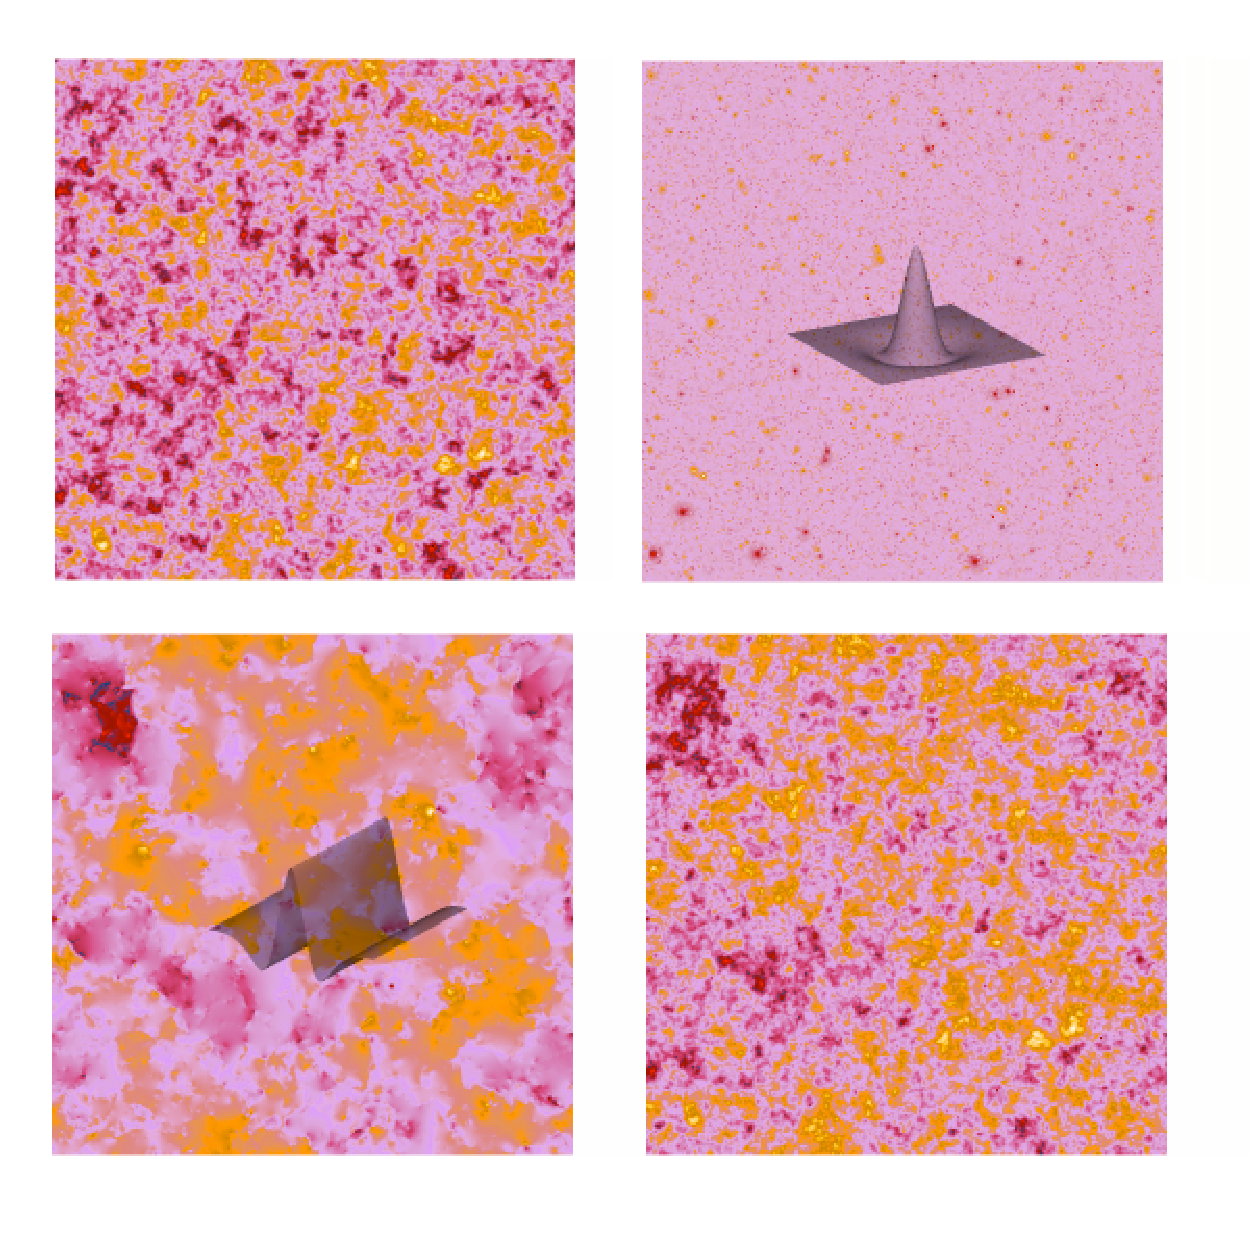
\includegraphics[width=13cm,height=13cm]{fig_cmbcssz.pdf}
\caption{Top, primary Cosmic Microwave Background anisotropies (left) and kinetic Sunyaev-Zel'dovich fluctuations (right). 
Bottom, cosmic string simulated map (left) and simulated observation containing the previous three components (right). 
The wavelet function is overplotted on the Sunyaev-Zel'dovich map and the curvelet function is overplotted on cosmic string map.}
\label{fig_cmb}
\end{figure}

In order to illustrate this, we show in Fig.~\ref{fig_cmb} a set of simulated maps. Primary CMB, kinetic SZ and cosmic string 
maps are shown respectively in Fig.~\ref{fig_cmb} top left, top right and bottom left. The ``simulated observed map", containing 
the three previous components, is displayed in Fig.~\ref{fig_cmb} bottom right. The primary CMB anisotropies dominate all the 
signals except at very high multipoles (very small angular scales). The wavelet function is overplotted on the kinetic Sunyaev-Zel'dovich 
map and the curvelet function is overplotted on cosmic string map.


CMB data are different from other astronomical data sets in the sense that they are not sparse (typical sparse data are stars or/and 
galaxies on top of a smooth background). After a component separation processing (see chapter~\ref{ch_mrs_ica}), the CMB data are not 
completely free of contaminations. Point sources still need to be detected and removed. Once we believe the data are clean enough, 
we want to check if the distribution of CMB temperature fluctuations is Gaussian by using robust statistical Gaussianity tests. 
\index{SZ effect}
\index{cosmic strings}
\index{CMB}

\section{Point Sources on a Gaussian Background}
\index{detection!point sources}
\index{wavelet!mexican hat}
\index{detection!matched filter}

Several methods have been proposed in the last years for point source detection in the CMB such as the the Mexican Hat wavelet \citep{gauss:cayon00,gauss:cayon01}, 
the pseudo-filter \citep{gauss:sanz01}, or the biparametric scale-adaptive filter \citep{gauss:sanz05}. A simple and robust technique, which maximizes 
the signal-to-noise ratio is the Matched Filter \citep{gauss:vio02}. Assuming an isotropic point spread function (PSF) with known power sprectum $\tau(q)$ 
and the CMB with power spectrum $P(q)$, the Matched Filter is \citep{gauss:vio02}:
\begin{equation} 
\label{eqn_mf}
\widehat{\psi}_{MF}(q) = \frac{1}{2 \pi \alpha}~ \frac{\tau(q)}{P(q)},\qquad \alpha \equiv \int_0^{+\infty}q \frac{\tau^2}{P} ~dq
\end{equation}
with minimum variance
\begin{equation} 
\sigma^2 = \frac{1}{2 \pi \alpha}
\end{equation}

\newpage
If the PSF is unknown (or space-variant), the Mexican Hat wavelet may be a good alternative. It consists of convolving the data 
with the wavelet function $\psi_{a,b} (x) =  \psi(\frac{x-b}{a})$, where $\psi(x)= \frac{1}{\sqrt{2\pi}}(1 - x^2) e^{- x^2/2}$. 
$a$ is the scale parameter and $b$ the position parameter. A fast implementation is obtained by using the Fourier transform to 
perform the convolution products ($\widehat{\psi}_{a}(q) = \frac{2}{\sqrt{\pi}} {(q a )}^2 e^{- \frac{1}{2}{(q a)}^2}$) \citep{gauss:sanz05}.




\section{Detecting Faint Non-Gaussian Signals Superposed on a Gaussian Signal}
\label{sec:Theory}
The superposition of a non-Gaussian signal with a Gaussian signal can be modeled as $Y = N + G$, where $Y$ is the observed image, 
$N$ is the non-Gaussian component and $G$ is the Gaussian component. We are interested in using transform coefficients to test 
whether $N \equiv 0$ or not.  

\subsection{Hypothesis Testing and Likelihood Ratio Test (LRT).}  
\label{subsec:LRT}
\index{statistic!LRT}

Transform coefficients of various kinds [Fourier, wavelet, curvelet, etc.] have been used for detecting non-Gaussian behavior 
in numerous studies. Let $X_1, X_2, \ldots, X_n$ be the transform coefficients of $Y$; we model these as  
\begin{equation}    
\label{EqAlt}
X_i = \sqrt{1 - \lam} \cdot  z_i + \sqrt{\lam} \cdot w_i,  \qquad 0< \lam < 1
\end{equation}
where $\lam >0$ is a parameter, $z_i \stackrel{iid}{\sim} N(0,1)$ are the transform coefficients of the Gaussian component $G$, 
$w_i \stackrel{iid}{\sim} W$ are the transform coefficients of the non-Gaussian component $N$, and $W$ is some unknown symmetrical 
distribution. Here without loss of generality, we assume the standard deviation for both $z_i$ and $w_i$ are $1$. 

Phrased in statistical terms, the problem of detecting the existence of a non-Gaussian component is equivalent to discriminating between the hypotheses:  
\begin{eqnarray}
\label{EqHypo2}
&H_0: \;\;\;   X_i = z_i  \label{EqHypo1}   \\
&H_1:   X_i = \sqrt{1 - \lam } \cdot z_i  + \sqrt{\lam} \cdot  w_i,   \qquad 0 < \lam < 1  
\end{eqnarray}
and $N \equiv 0$ is equivalent to $\lam \equiv 0$. We call $H_0$ the {\it null hypothesis $H_0$}, and $H_1$ the {\it alternative hypothesis}. 

% \begin{figure}
% \centering
% \includegraphics[height = 3 in]{PDF/CSDetectRegion.pdf}
% \caption{Detectable regions  in the $\alpha-r$ plane.  With $(\alpha,r)$ in the white region on the top or the undetectable region, all methods completely fail for detection. With $(\alpha,r)$ in the white region on the bottom,  both excess kurtosis and Max/HC are able to detect reliably.      While in the blue region to the left,  Max/HC is able to detect reliably, but excess kurtosis completely fails, and in the yellow region to the right, excess kurtosis is able to detect reliably, but Max/HC  completely fail.     }
% \label{Figure:Detect}
% \end{figure}

\begin{figure}[htb]
\centerline{
\hbox{
\includegraphics[width=12cm]{CSDetectRegion.pdf}%,height=12cm
% \psfig{figure=,bbllx=1.5cm,bblly=8.cm,bburx=19.5cm,bbury=23cm,height=6cm,width=7.5cm,clip=}
 }}
\caption{Detection Boundary in the $\alpha-r$ plane. The solid curve is the detection boundary of LRT, above which is not possible to detect, 
and below which it is possible to reliably detect, the dotted line segment and solid line segment together is the detection boundary for Kurtosis, 
the dotted curve and the solid curve together is the detection boundary of Max/HC. Right panel: detectable regions for Kurtosis, Max/HC.}
\label{Figure:Detect}
\end{figure}

When both $W$ and $\lam$ are known, then the optimal test for Problem (\ref{EqHypo1}) - (\ref{EqHypo2}) is simply 
the Neyman-Pearson Likelihood ratio test (LRT), \cite[Page 74 ]{Lehmann}. The size of $\lam = \lam_n$  for which 
reliable discrimination between $H_0$ and $H_1$ is possible can be derived using asymptotics. If we assume that 
the tail probability of $W$ decays algebraically, 
\begin{equation} \label{EqDefineAlg}
\lim_{x \goto \infty}   x^{\alpha}  P\{|W| > x\}  = C_{\alpha},  \qquad \mbox{$C_{\alpha}$ is a constant}
\end{equation}
(we say $W$ has a power-law tail), and we calibrate $\lam$ to decay with $n$, so that increasing amounts of data are offset by increasingly hard challenges: 
\begin{equation}   \label{EqDefineLam}
\lam = \lam_n  = n^{-r}  
\end{equation}
then there is a {\it threshold effect} for the detection problem (\ref{EqHypo1}) - (\ref{EqHypo2}). In fact, define:\\
\begin{equation} \label{EqDetectBoundary}
\rho^*_1(\alpha) = 
\left\{ \begin{array}{ll}
2/\alpha, &\   \  \alpha \leq 8 \\
1/4, &\     \       \alpha > 8
\end{array}
\right.
\end{equation}
then as $n \goto \infty$, LRT is able to reliably detect for large $n$ when $r < \rho^*_1(\alpha)$, and is unable to detect 
when $r > \rho^*_1(\alpha)$; this is proved in \citep{DJ04b}. Since LRT is optimal, it is not possible for any statistic to 
reliably detect when $r > \rho^*_1(\alpha)$. We call the curve $r = \rho^*_1(\alpha)$ in the $\alpha$-$r$ plane the 
{\it detection boundary}; see Figure \ref{Figure:Detect}.\\

In fact, when $r < 1/4$, asymptotically LRT is able to reliably detect whenever $W$ has a finite $8$-th moment, even without 
the assumption that $W$ has a power-law tail. Of course, the case that $W$ has an infinite $8$-th moment is more complicated, 
but if $W$ has a power-law tail, then LRT is also able to reliably detect if $r < 2/\alpha$. 

% One component of the above result is that, by assuming  $W$ has an 
% $\alpha$-algebraic tail 
% with $\alpha > 8$, then when $r < \frac{1}{4}$,  LRT is 
% able to reliably detect;  
% and when $r > \frac{1}{4}$, no statistic is able to detect.  
% It is interesting to notice here that, this part of the conclusion will still hold 
% when  
% the condition of requiring $W$ to have an algebraic tail is largely relaxed:  in 
% fact,  the same conclusion still holds if we only require $E[W^8] < \infty$.  It is 
% interesting to notice here that,  when $W$ has an $\alpha$-algebraic tail, 
% $E[W^8] < \infty$ if and only if $\alpha > 8$.

Despite its optimality, LRT is not a practical procedure. To apply LRT, one needs to specify the value of $\lam$ and 
the distribution of $W$, which seems unlikely to be available. We need non-parametric detectors, which can be implemented 
without any knowledge of $\lam$ or $W$, and depend on $X_i$'s only. In the next section, we are going to introduce three 
non-parametric detectors: excess kurtosis, Max and Higher Criticism (HC).   

\section{Kurtosis, HC from Wavelet and Curvelet Coefficients}
 
\subsection{Kurtosis}
\index{statistic!Kurtosis}
\index{Kurtosis}

For a statistic $T_n$, the $p$-value is the probability of seeing equally extreme results under the null hypothesis:
\[
p = P_{H_0} \{ T_n  \geq t_n(X_1,X_2, \ldots,X_n) \}
\] 
here $P_{H_0}$ refers to probability under $H_0$, and $t_n(X_1,X_2, \ldots,X_n)$ is the observed value of statistic $T_n$. 
Notice that the smaller the $p$-value, the stronger the evidence against the null hypothesis. A natural decision rule based 
on $p$-values rejects the null when $p < \alpha$ for some selected level $\alpha$, and a convenient choice is  $\alpha = 5\%$. 
When the null hypothesis is indeed true, the $p$-values for any statistic are distributed as uniform $U(0,1)$. This implies 
that the $p$-values provide a common scale for comparing different statistics. 

We now introduce two statistics for comparison. 

{\bf Excess Kurtosis ($\kappa_n$)}. Excess kurtosis is a widely used statistic, based on the $4$-th moment. 
For any (symmetrical) random variable $X$, the kurtosis is:
\[
\kappa(X) = \frac{EX^4}{(EX^2)^2} -3
\]
The kurtosis measures a kind of departure of $X$ from  Gaussianity, as $\kappa(z) =  0$.
Empirically, given $n$ realizations of $X$, the excess kurtosis statistic is defined as: 
\begin{equation}  \label{EqDefineK}
\kappa_n(X_1, X_2,\ldots,X_n)  = \sqrt{\frac{n}{24}} \biggl[ \frac{\frac{1}{n}\sum_i  X_i^4}{(\frac{1}{n}  \sum_i X_i^2)^2}  - 3  \biggr]
\end{equation} 
When the null is true, the excess kurtosis statistic is asymptotically normal:
\[
\kappa_n(X_1, X_2,\ldots,X_n)  \rightarrow_{w}  N(0,1), \qquad n \goto \infty
\]
thus for large $n$, the $p$-value of the excess kurtosis is approximately:
\[
\tilde{p} = \bar{\Phi}^{-1} (\kappa_n(X_1, X_2,\ldots,X_n))
\]
where $\bar{\Phi}(\cdot)$ is the survival function (upper tail probability) of $N(0,1)$. 

It is proved in \citep{DJ04b} that the excess kurtosis is asymptotically optimal for the hypothesis testing of \eqref{EqHypo1} - \eqref{EqHypo2} if 
\[
E [W^8] < \infty
\]
However, when $E[W^8] = \infty$, even though kurtosis is well-defined ($E[W^4] < \infty$), there are situations in which LRT 
is able to reliably detect but excess kurtosis completely fails. In fact, by assuming \eqref{EqDefineAlg} - \eqref{EqDefineLam} 
with an $\alpha < 8$, if $(\alpha,r)$ falls into the blue region of Figure~\ref{Figure:Detect}, then LRT is able to reliably detect, 
however, excess kurtosis completely fails. This shows that in such cases, excess kurtosis is not optimal; see \citep{DJ04b}. 

\subsection{Max}
\index{statistic!max}
\index{max}
The largest (absolute) observation is a classical and frequently-used non-parametric statistic:
\[
M_n =  \mmax(|X_1|,|X_2|,\ldots, |X_n|)
\] 
under the null hypothesis, 
\[
M_n  \approx \sqrt{2 \log n}
\]
and moreover, by normalizing $M_n$ with constants $c_n$ and $d_n$, the resulting statistic 
converges to the Gumbel distribution $E_v$, whose cdf is $e^{-e^{-x}}$:
\[
\frac{M_n - c_n}{d_n}  \rightarrow_{w}    E_v
\]
where approximately
\[
d_n = \frac{\sqrt{6} S_n}{\pi}, \qquad  c_n = \bar{X} - 0.5772 d_n 
\]
here $\bar{X}$ and $S_n$ are the sample mean and sample standard deviation of $\{X_i\}_{i=1}^n$ respectively. 
Thus a good approximation of the $p$-value for $M_n$ is:
\[
\tilde{p} =  \mathrm{exp}(-\mathrm{exp}(-\frac{M_n - c_n}{d_n}))
\]
We have tried the above experiment for $n = 244^2$, and found that taking $c_n = 4.2627$, $d_n = 0.2125$ gives a good approximation.  

Assuming \eqref{EqDefineAlg} - \eqref{EqDefineLam} and $\alpha < 8$, or $\lam = n^{-r}$ and that $W$ has a power-law tail 
with $\alpha < 8$, it is proved in \citep{DJ04b} that Max is optimal for hypothesis testing \eqref{EqHypo1} - \eqref{EqHypo2}. 
Recall if we further assume $\frac{1}{4} < r < \frac{2}{\alpha}$, then asymptotically, excess kurtosis completely fails; 
however, Max is able to reliably detect and is competitive to LRT. 

On the other hand, recall that excess kurtosis is optimal for the case $\alpha > 8$. In comparison, in this case, 
Max is not optimal. In fact, if we further assume $ \frac{2}{\alpha} < r < \frac{1}{4}$, then  excess kurtosis 
is able to reliably detect, but Max will completely fail. 

In Figure \ref{Figure:Detect}, we compared the detectable regions of the excess kurtosis and Max in the $\alpha$-$r$ plane. 

\subsection{Higher Criticism}
\label{sec:HC}
\index{statistic!Higher Criticism}
\index{Higher Criticism}

The Higher Criticism statistic (HC), was proposed in \citep{gauss:lin02}. To define HC first we convert the individual $X_i$'s 
into $p$-values for individual $z$-tests. Let $p_i = P\{ N(0,1) > X_i \}$ be the $i^{th}$ $p$-value, and let $p_{(i)}$ denote 
the $p$-values {\it sorted in increasing order}; the Higher Criticism statistic is defined as:
\[
       HC_{n}^* =  \max_{i}
         \biggl| \sqrt{n} [i/n  - p_{(i)}]/ \sqrt{p_{(i)} (1-p_{(i)})} \biggr|
\]
or in a modified form:
\[
HC_n^+  = \max_{\{i:  \; 1/n  \leq  p_{(i)} \leq  1 - 1/n \}}
         \biggl|   \sqrt{n} [i/n  - p_{(i)}]/ \sqrt{p_{(i)} (1-p_{(i)})}  \biggr|
\]
we let $HC_n$ refer either to $HC_n^*$ or $HC_n^+$ whenever there is no confusion. The above definition is slightly 
different from \citep{gauss:lin02}, but the ideas are essentially the same.

With an appropriate normalization sequence:
\[
a_n = \sqrt{2 \log \log n}, \qquad b_n = 2 \log \log n + 0.5 \log \log \log n - 0.5 \log (4 \pi)
\]
the distribution of $HC_n$ converges to  the Gumbel distribution $E_v^4$, whose cdf is $\mathrm{exp}(-4\mathrm{exp}(-x))$, \citep{Shorack}:
\[
a_n  HC_n - b_n  \rightarrow_w  E_v^4
\]
so the $p$-values of $HC_n$ are approximately:
\begin{equation}  
\label{EqHCP}
\mathrm{exp}(-4\mathrm{exp}( - [a_n HC_n - b_n]))
\end{equation}
For moderately large $n$, in general, the approximation in \eqref{EqHCP} is accurate for the $HC_n^+$, but not for $HC_n^*$.   

A brief remark comparing Max and HC. Max only takes into account the few largest observations, HC takes into account those outliers, 
but also moderate large observations. As a result, in general HC is better than Max, especially when we have unusually many moderately 
large observations. However, when the actual evidence lies in the middle of the distribution both HC and Max will be very weak.

% \section{The Genus and the Multiscale Genus}

\section{Experiments}

\begin{figure}[htb]
\vbox{
\centerline{
\hbox{
 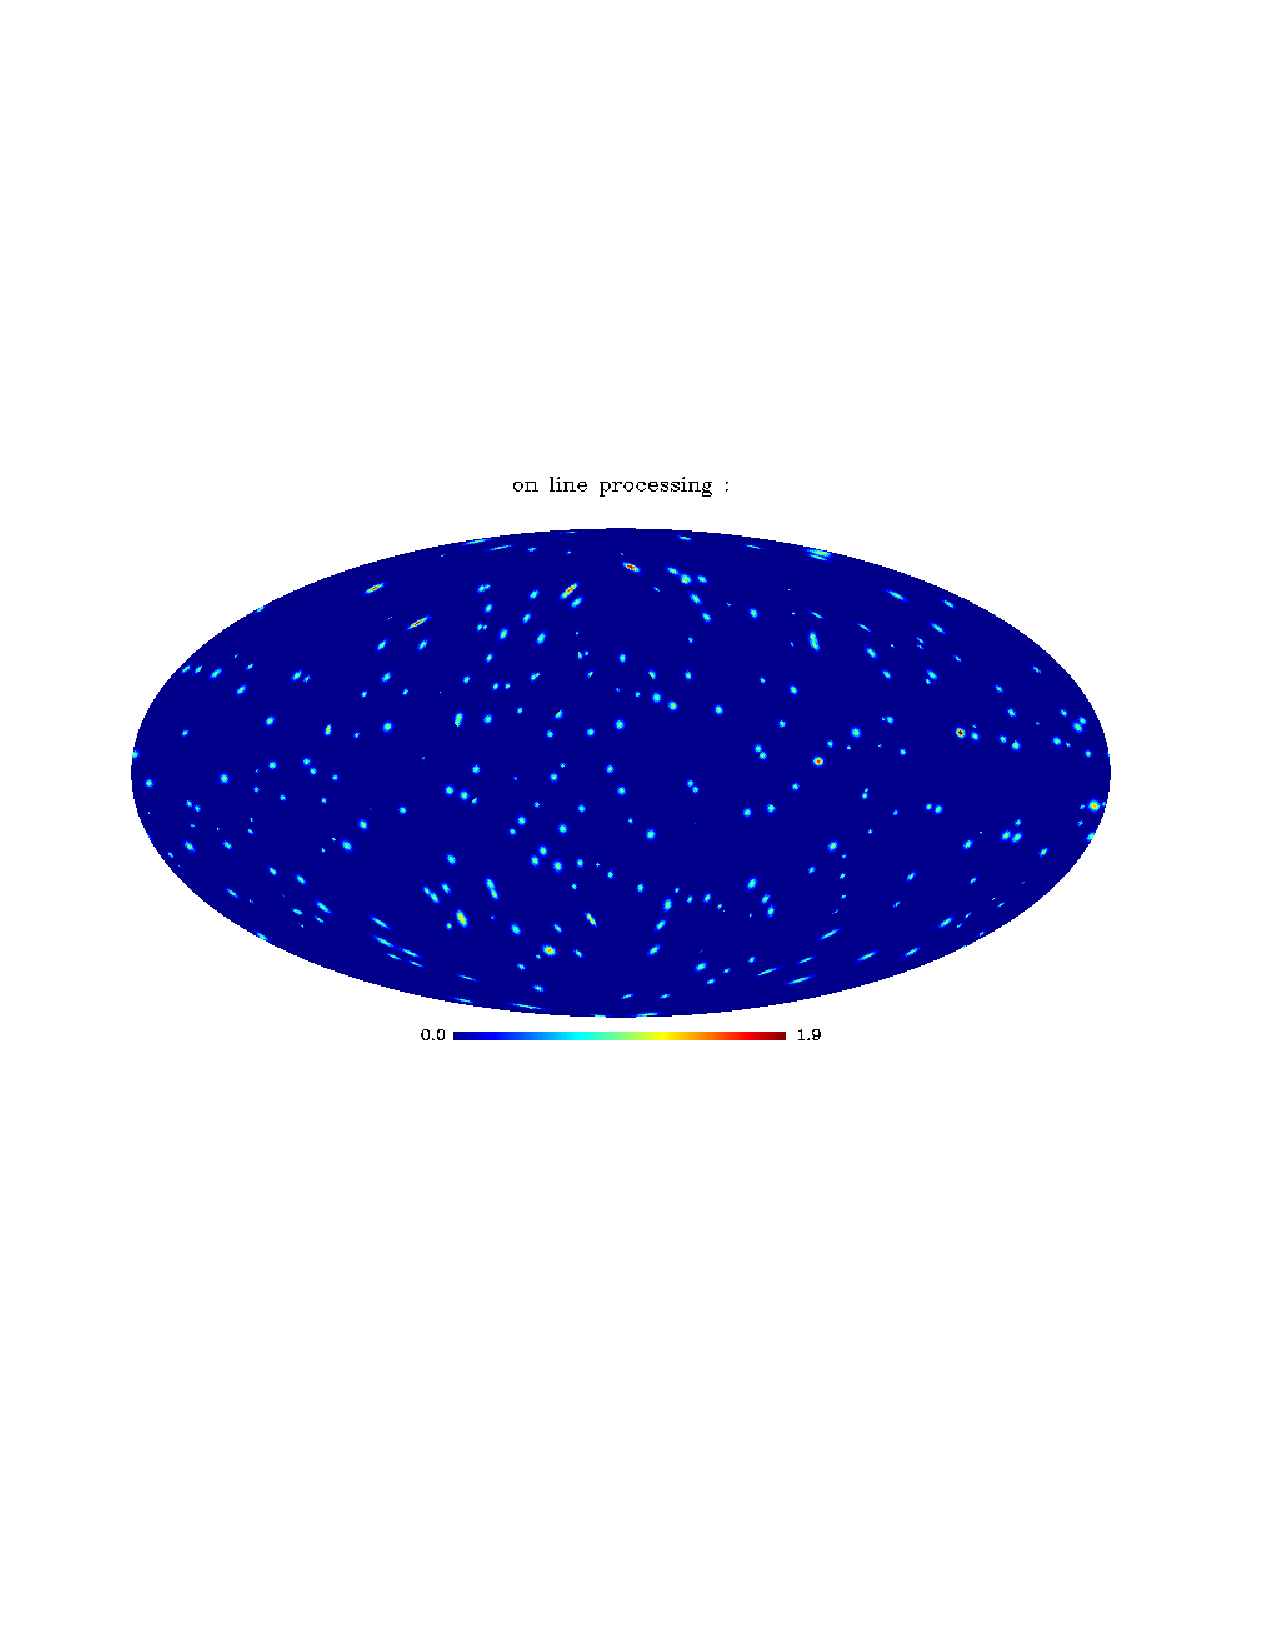
\includegraphics[trim= 2cm 8cm 2cm 8cm,width=7.9cm]{fig_sphere_gaussian.pdf}%[width=8.5cm,height=4.5cm]
 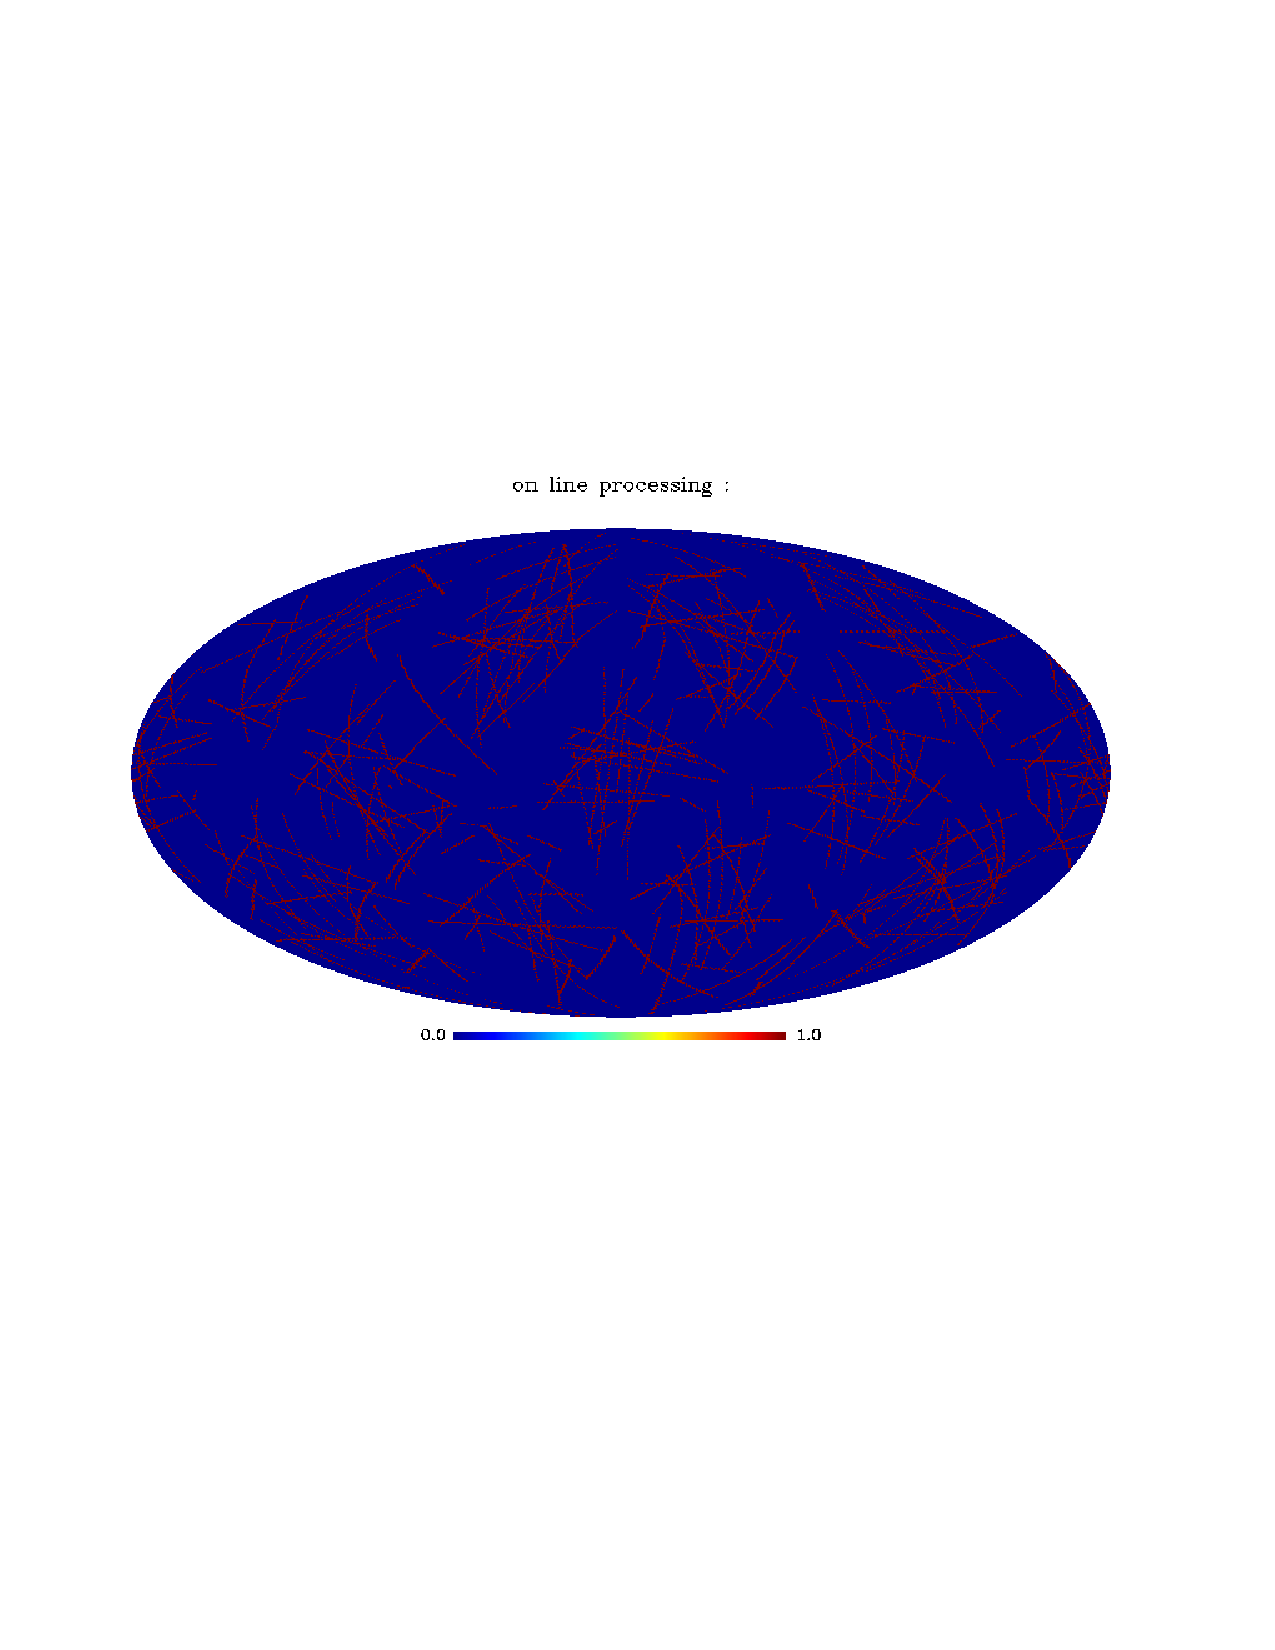
\includegraphics[trim= 2cm 8cm 2cm 8cm,width=7.9cm]{fig_sphere_line.pdf}
}}
 \centerline{
 \hbox{
 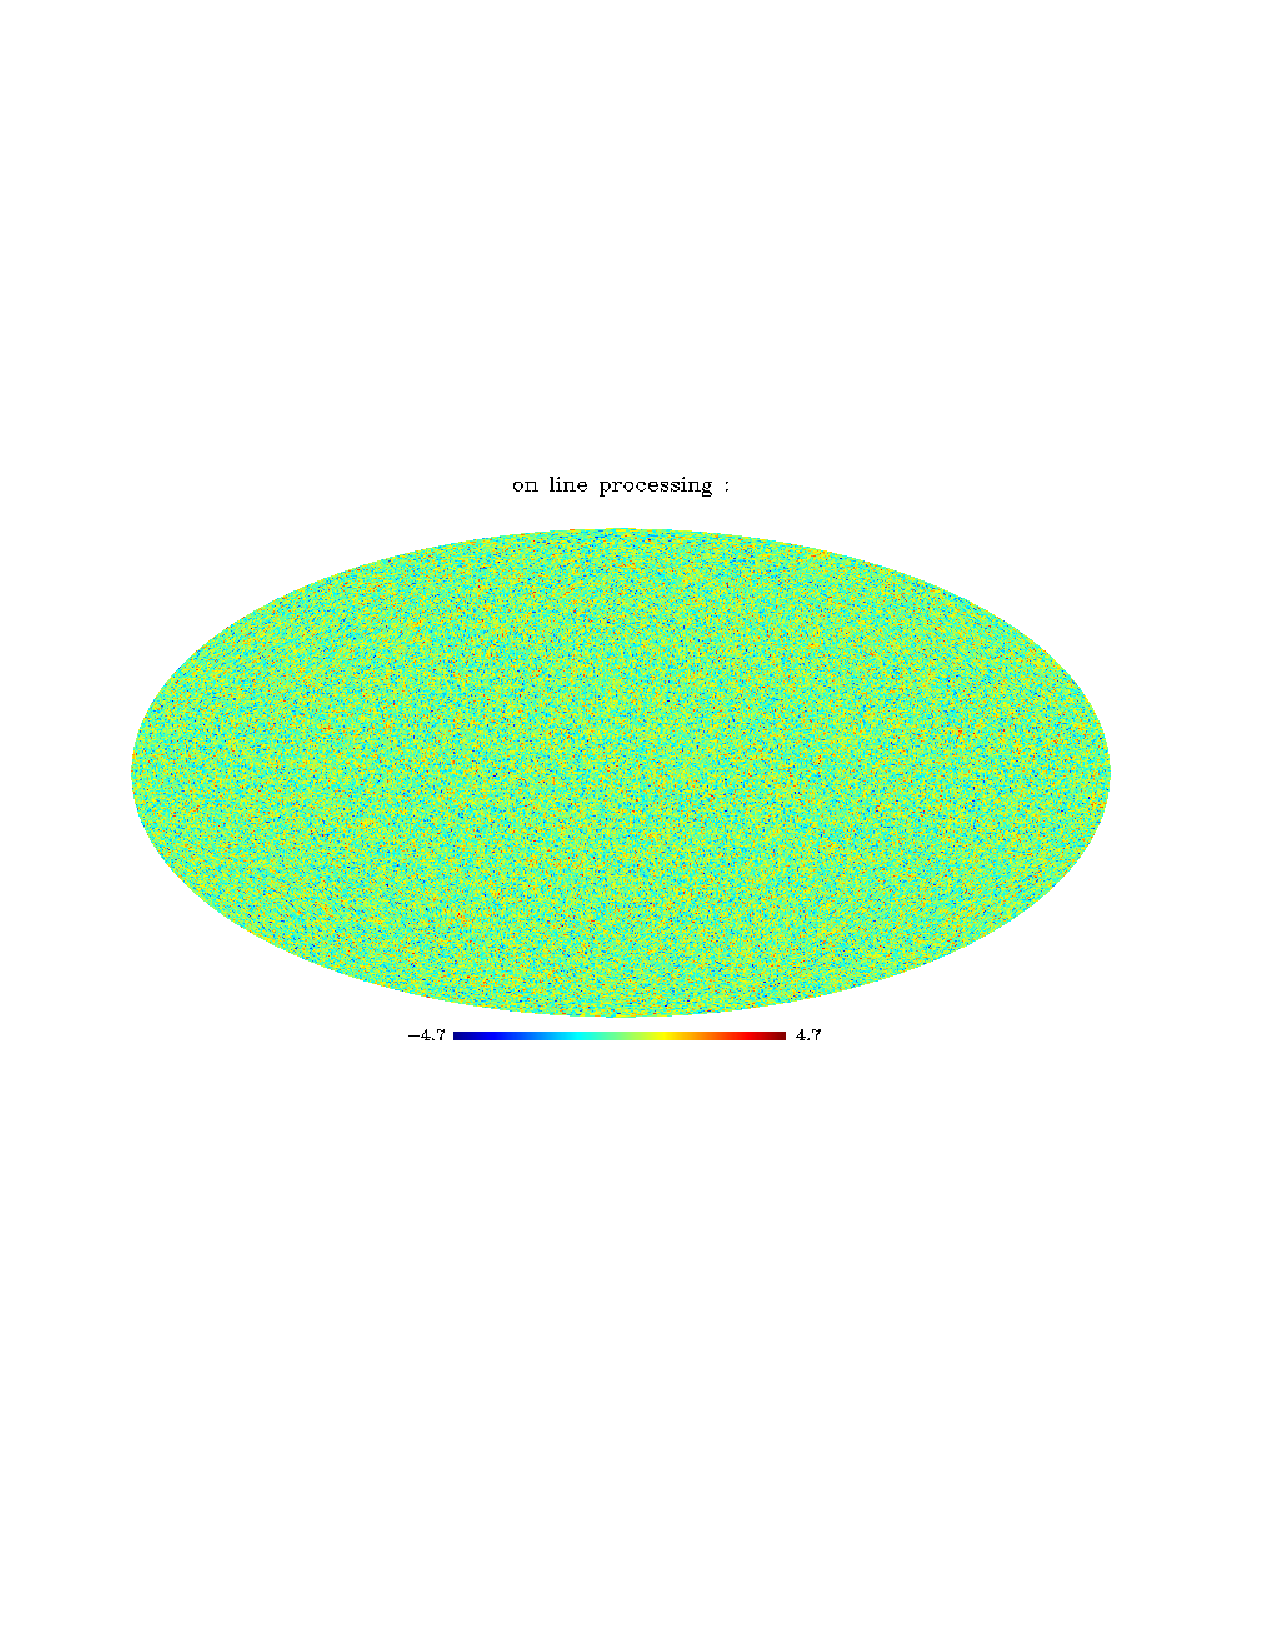
\includegraphics[trim= 2cm 8cm 2cm 8cm,width=7.9cm]{fig_sphere_gaussian_noise_snr1.pdf}
 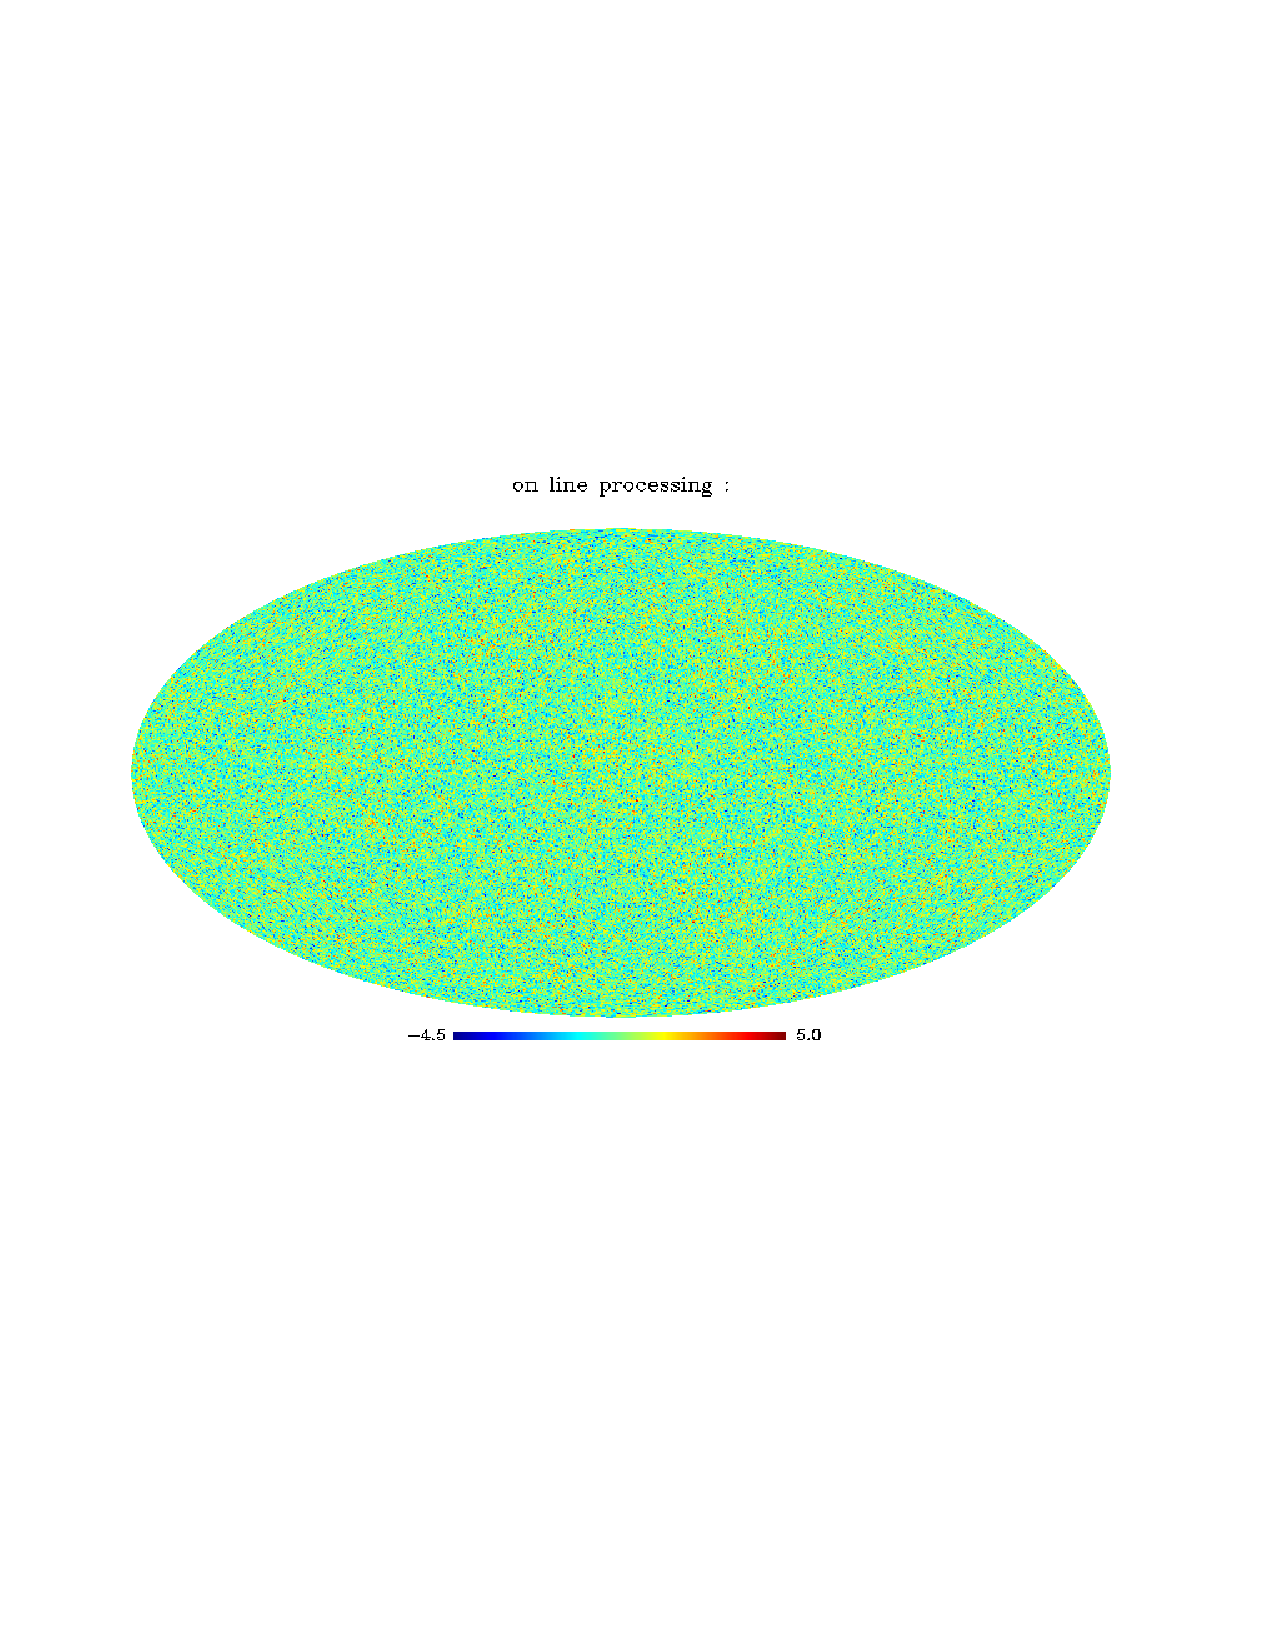
\includegraphics[trim= 2cm 8cm 2cm 8cm,width=7.9cm]{fig_sphere_line_noise_snr1.pdf}
}}}
 \caption{Top, image with Gaussians and image with lines. Bottom, same images but with an additional Gaussian noise. The SNR is equal to 1.}
\label{fig_sphere_linegauss}
\end{figure}

Fig.~\ref{fig_sphere_linegauss} shows, top left and right, two images with respectively Gaussians and lines. We have created a set 
of simulated images by adding a Gaussian white noise with different standard deviations to these two images. The Signal to Noise 
Ratio (SNR) varies between 0 and 1. For the image with lines, the SNR is defined as the pixel values along the lines divided by the 
noise standard deviation, and  for the image with Gaussians, the SNR is defined as the maximum of the Gaussians divided by the noise 
standard deviation. Fig.~\ref{fig_sphere_linegauss} shows, bottom left and right, the two noisy images with a SNR equal to 1. Hence, 
for each SNR value, we have thirty realizations of the noise, and we have calculated the kurtosis at the different scales of both the 
curvelet and the wavelet coefficients. These kurtosis values were normalized by the standard deviation of the kurtosis obtained from 
the wavelet and the curvelet transform of thirty Gaussian white noise realizations. Finally we kept for each SNR the maximum normalized 
kurtosis along the scales. Fig.~\ref{fig_wtcur_sphere_linegauss} left (resp.~right) shows the normalized kurtosis values using the wavelet 
transform (resp. the curvelet transform) for the two images (i.e. lines and Gaussians) versus the SNR. Continuous error bars correspond 
to $1\sigma$ level and dashed error bars correspond to $2\sigma$ level. We can clearly see that the detection power of the wavevet 
transform is much larger than the detection power of the curvelet transform for detecting non-Gaussianities due to isotropic features, 
while curvelets are more powerful than wavelets for detecting anisotropic features.

\begin{figure}[htb]
\centerline{
 \hbox{
% {figure=,bbllx=2.5cm,bblly=12.5cm,bburx=19.5cm,bbury=25.5cm,width=8.5cm,height=6.5cm,clip=}
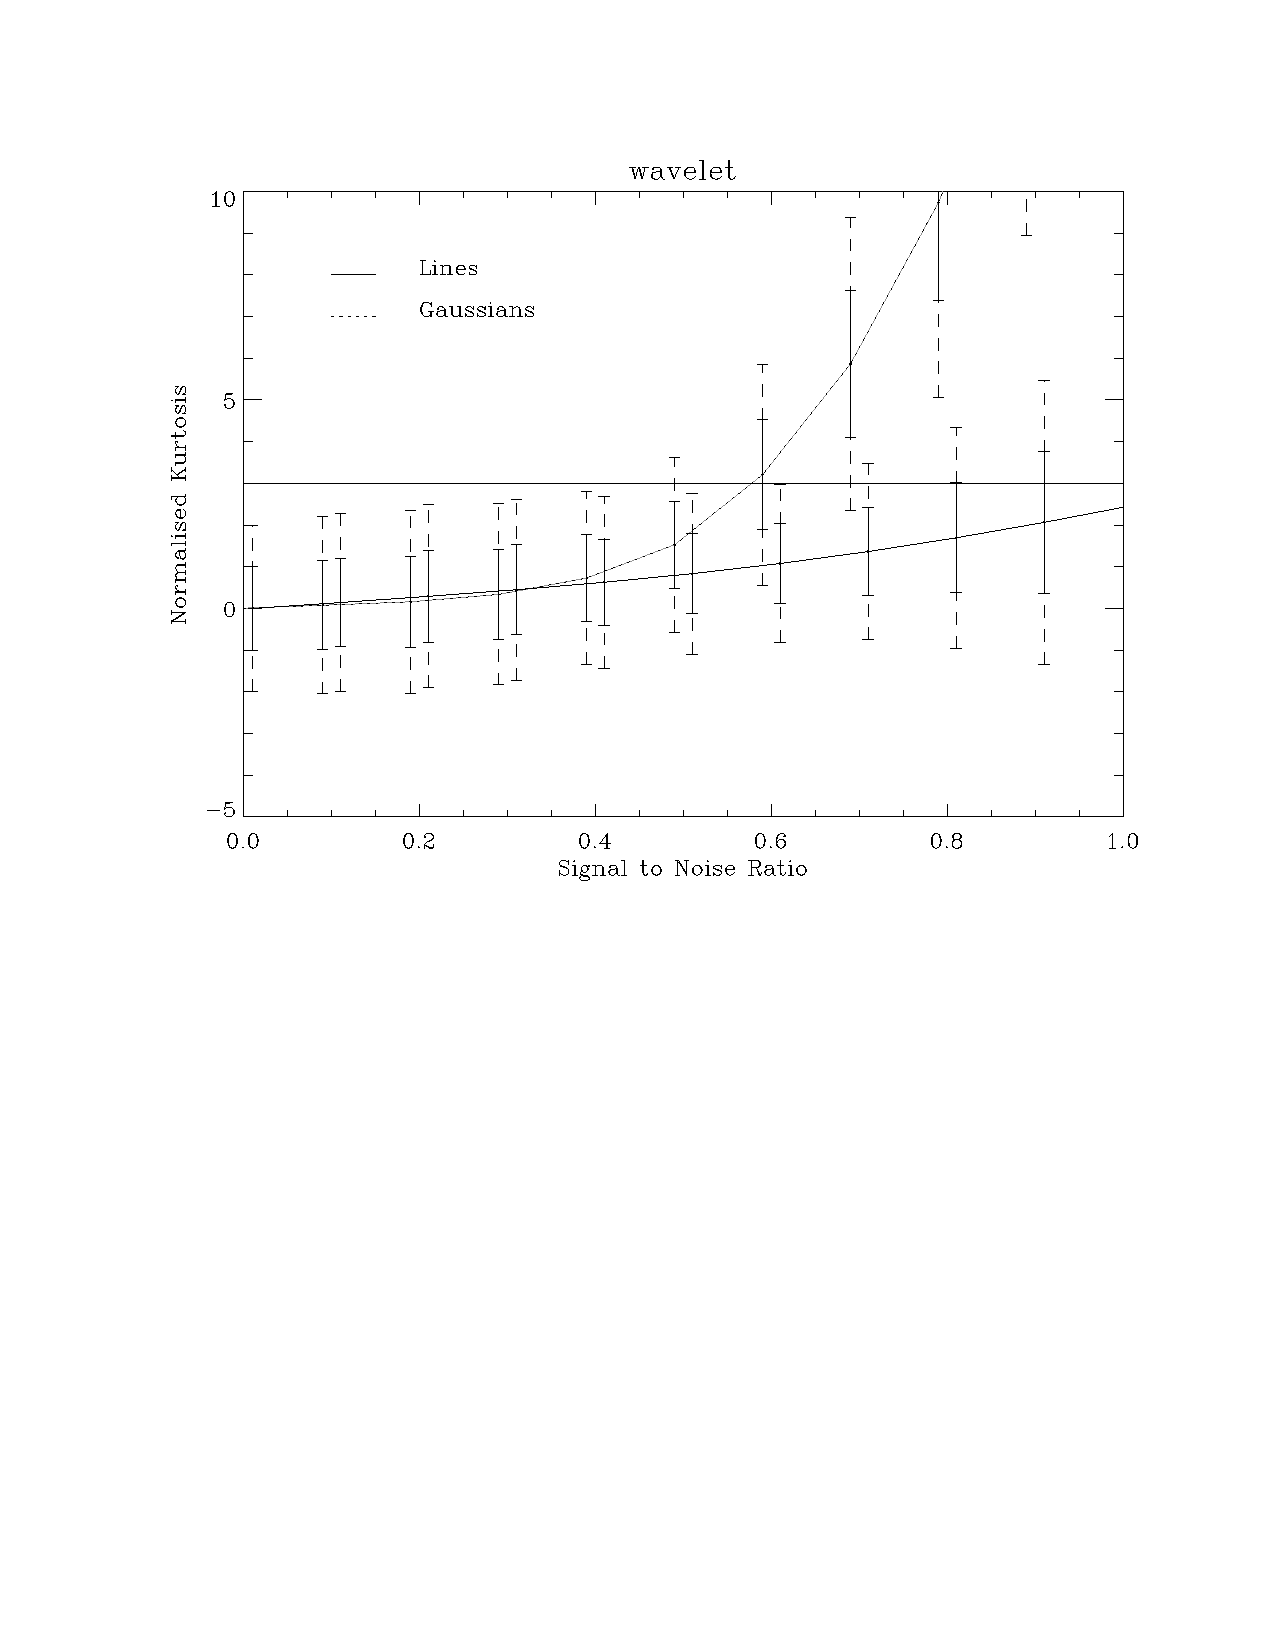
\includegraphics[trim= 2cm 13cm 2cm 3cm,width=7.9cm]{fig_sphere_wt_linedroite.pdf}%,height=6.5cm
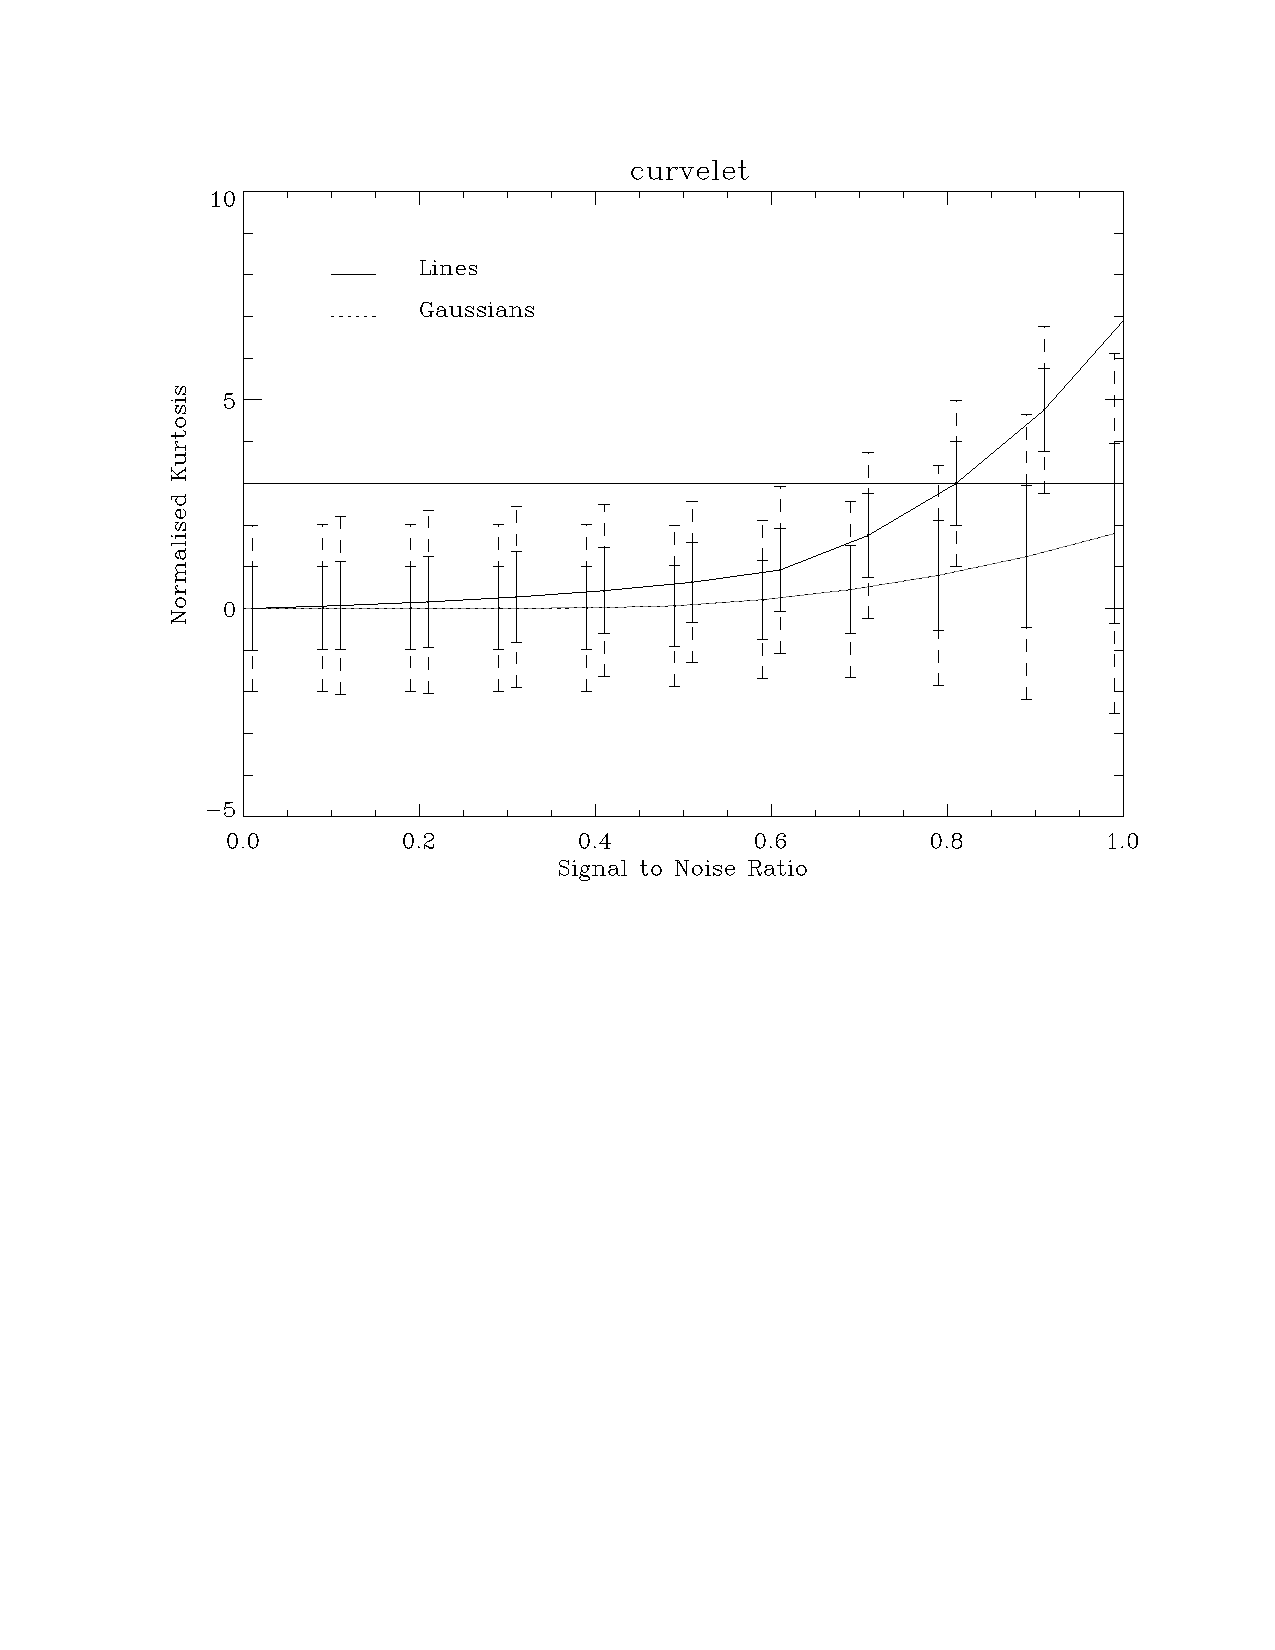
\includegraphics[trim= 2cm 13cm 2cm 3cm,width=7.9cm]{fig_sphere_cur_linedroite.pdf}
% \psfig{figure=fig_sphere_cur_linedroite.pdf,bbllx=2.5cm,bblly=12.5cm,bburx=19.5cm,bbury=25.5cm,width=8.5cm,height=6.5cm,clip=}
}}
\caption{Normalised kurtosis value versus the SNR for the wavelet coefficients (left) and the curvelet coefficients (right). 
The continuous error bars correspond to one $\sigma$ and the dashed error bars correspond to $2\sigma$.}
\label{fig_wtcur_sphere_linegauss}
\end{figure}

\section{Conclusions}
\index{wavelet!Kurtosis}
\index{wavelet!Higher Criticism}
\index{curvelet!Kurtosis}
\index{curvelet!Higher Criticism}
\index{SZ effect}
\index{cosmic strings}
\index{detection!non-Gaussianity}

The kurtosis of the wavelet coefficients is very often used in astronomy for the detection of non-Gaussianities in the CMB. It has been 
shown \citep{starck:sta03_1} that it is also possible to separate the non-Gaussian signatures associated with cosmic strings from those 
due to SZ effect by combining the excess kurtosis derived from these both the curvelet and the wavelet transform. It has been shown that 
kurtosis is asymptotically optimal in the class of weakly dependent symmetric non-Gaussian contamination with finite 8-th moments, while 
HC and MAX are asymptotically optimal in the class of weakly dependent symmetric non-Gaussian contamination with infinite 8-th moment \citep{starck:jin05}. 
Hence depending on the nature of the non-Gaussianity, a statitic is better than another one. This is a motivation for using several statistics 
rather than a single one for analysing CMB data. The case of the detection of cosmic string contaminations has been studied on simulated maps, 
and it has been shown that kurtosis outperforms clearly Max/HC \citep{starck:jin05}.  




  

\section{IDL Routines}
\label{ch_mrs_idl}
%\chapterhead{IDL Routines}
\markright{IDL Routines}

\subsection{Introduction}
A set of routines has been developed in IDL. Starting IDL using
the script program {\em mre} allows the user to get the multiresolution
environment, and all routines
described in the following can be called. An online help facility 
is also available by
invoking the {\em mrh} program under IDL.

\subsection{mw1d\_filter}
Filter a 1D signal by the the multiscale entropy.
{\bf
\begin{center}
     USAGE: mw1d\_filter, Signal, Result, Opt=Opt
\end{center}}
where 
\begin{itemize}
\item {\em Signal}: input  one-dimensional IDL array.
\item {\em Result}: output one-dimensional IDL array (filtered signal).
\item {\em Opt}:  string which contains the different options 
(see the {\em mw1d\_filter} C++  program).
\end{itemize}

\subsection{mw1d\_predict}
Considering a temporal signal $S$ with $n$ measures ($S[0..n-1]$), 
 {\em mr1d\_predict} estimates (or predicts) the next values $S[n .. n+dt]$.
A multiscale transformation is first applied, followed by filtering
in the wavelet space. At each scale, a predictor is then applied,
and the predicted signal is obtained from the reconstruction of
the predicted signal. 

{\bf
\begin{center}
     USAGE: Result = MW1D\_PREDICT(Signal,wave=wave,PredWave=PredWave,
                      NPredict=NPredict, Nscale=Nscale,  OPT=OPT, NCoef=NCoef)
\end{center}}
where 
\begin{itemize}
\item {\em wave}: output 2D IDL array; filtered wavelet coefficient
\item {\em PredWave}: output 2D IDL array; Predicted wavelet coefficient
\item {\em NPredict}: number of values to predict. Default is one.
\item {\em Nscale}: number of scales used for the wavelet transform
\item {\em NCoef:} Number of coefficients used for the prediction. Default is 3.
\item {\em OPT}: string which contains the differents options accepted by the
mw1d\_filter C++ program.
\end{itemize}

\subsection{mw\_filter}
Filter  an image by the multiscale entropy. 
This routine is calling the C++ executable {mw\_filter}. The keyword 
``OPT" allows 
all options described in the section corresponding to the 
 {\em mw\_filter} program.

{\bf
\begin{center}
     USAGE: mw\_filter, Data, FilterData, opt=opt
\end{center}}
{\em Data} is an image (2D IDL array), and {\em FilterData} is the result
of the filtering.

\subsection{mw\_deconv}
Deconvolve an image by  the  multiscale entropy. This routine calls 
the C++ executable {mw\_deconv}. The keyword ``OPT" 
allows 
all options described in the section corresponding to the 
 {\em mw\_deconv} program.

{\bf
\begin{center}
     USAGE: mw\_deconv, Data, PSF, DeconvData, opt=opt
\end{center}}
\subsubsection*{Examples:} 
\begin{itemize}
\item mw\_deconv, Imag, Psf, Result \\
deconvolve an image with all default options.
\item  mw\_deconv, Imag, Psf, Result, OPT='-i 30 -e 0'  \\
same example, but impose the number of iterations to be 30.
\end{itemize}

 
  

\part{\projpol: \defprojpol }
   
\chapter{Multiscale Methods for polarized maps on the Sphere}
\label{ch_mms_pola}

% chapter multiscale transform for pola data

\section{Module-phase non linear multiscale transform}
%---------------------------------------------------------------------------------------------------------------------------------------
\label{sec:modphase}

\subsection{Introduction}
Given a polarized map in the standard Q-U representation, consider a different point of view and define the modulus $M$ and phase $P$ maps as follows~:
%
%From a different point of view, the combined $Q$ and $U$ maps can be considered as a vector field. Let define such combined map $\mathcal{V}$ as follows~:
%\begin{equation}
%{\mathcal{V}} = \left[ Q \, U\right]
%\end{equation}
%Each pixel of $\mathcal{V}$ is then vector valued. A classical approach amounts to decomposing each vector into its modulus and phase part. $\mathcal{V}$ can then be decomposed into a modulus map $M$ and a phase map $P$~:
\begin{eqnarray}
\forall k,\,\,\, M_k & = & \sqrt{Q_k^2 +  U_k^2} \\
\forall k,\,\,\, P_k & = & \exp(i \theta_k) \mbox{ where } tan(\theta_k) = U_k/Q_k 
\end{eqnarray}
Because the smoothness of the $Q$ and $U$ maps should result in some smoothness of the modulus map $M$ and the phase map $P$, 
one may consider devising a multiscale modulus/phase decomposition of the spin 2 field ${\mathcal{V}} = \left[ Q \, U\right]$.\\

The specificity of the modulus/phase decomposition of $\mathcal{V}$ is twofold~: i) the modulus field is non-negative and ii) the phase 
field takes its values on the unit circle $S^1$. Recently, \cite{rahman05} introduced a multiscale analysis technique for manifold valued 
data that will be described in the following paragraph. We then define the modulus/phase (MP) multiscale transform as follows~:
\vspace{.1cm}
\begin{center}
\begin{minipage}[b]{0.85\linewidth}
\footnotesize{
\begin{enumerate}
\item Apply a classical multiscale transform (\textit{i.e.} wavelets) to the modulus map $M$.
\item Apply the multiscale analysis technique for manifold valued data described in \cite{rahman05} to the phase map $P$. 
\end{enumerate}}
\end{minipage}
\end{center}
\vspace{.1cm}

\subsection{Decimated MP-multiscale transform}

\begin{figure*}[htb]
\centerline{
 \vbox{
 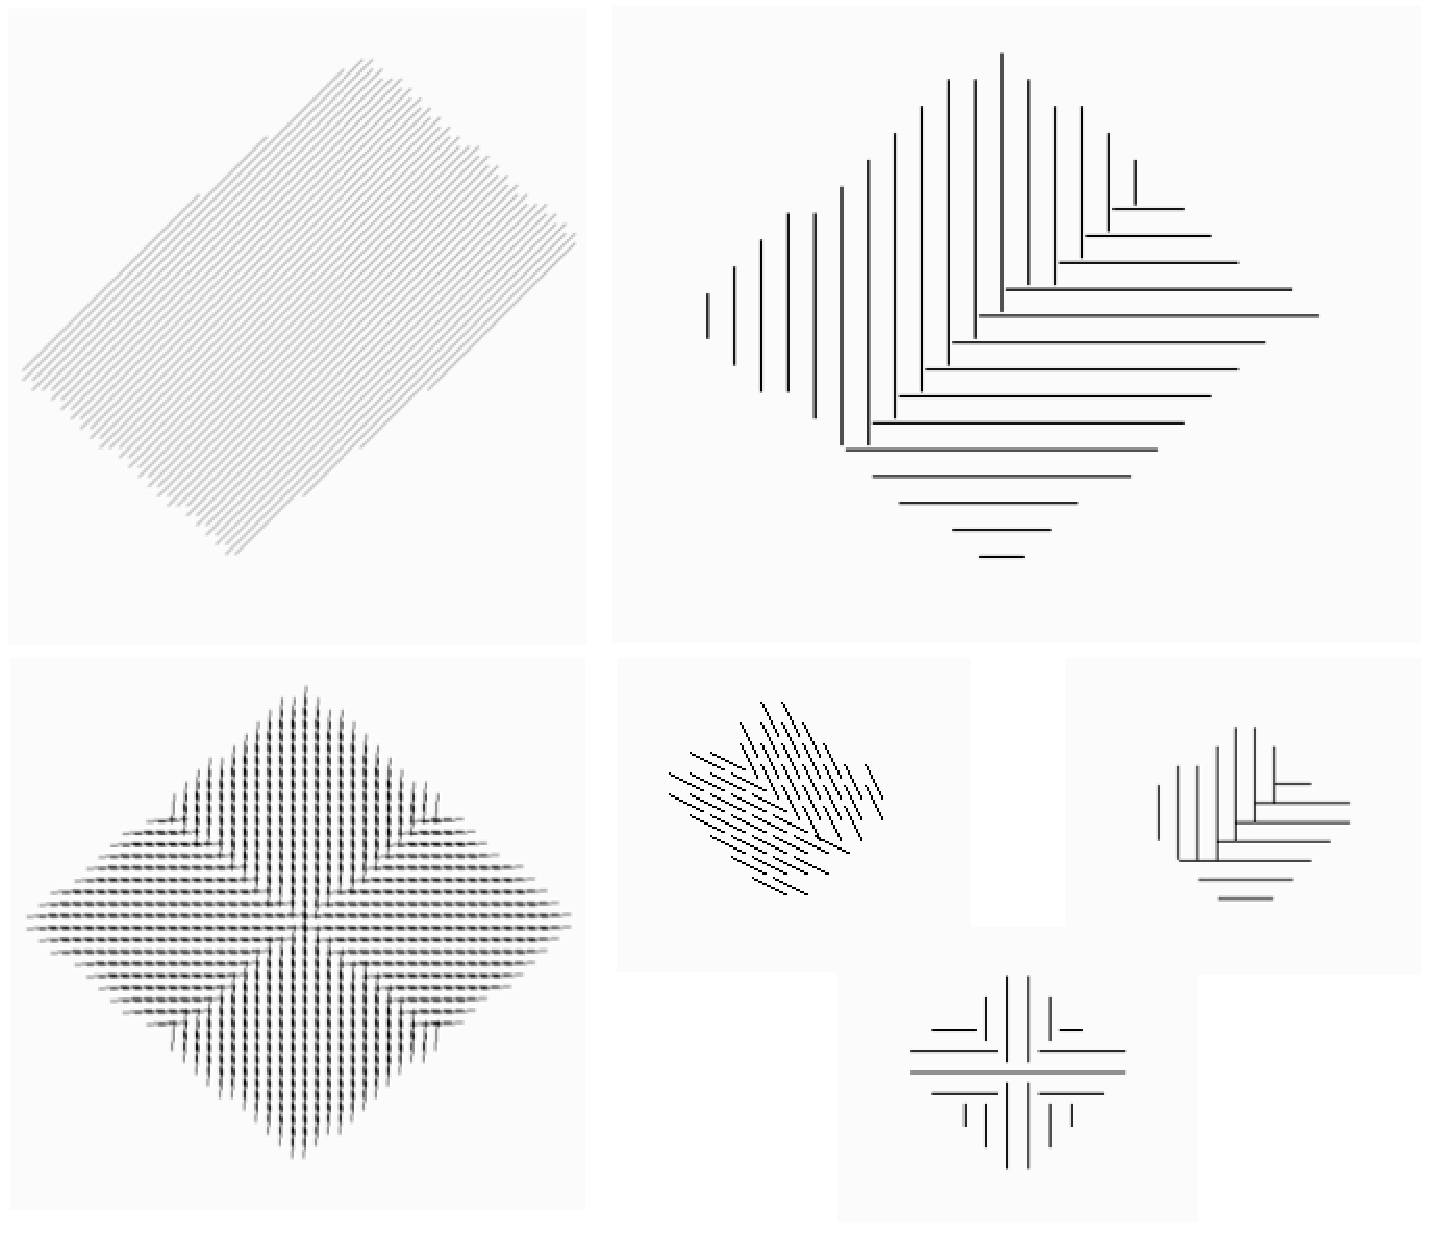
\includegraphics[width=\textwidth]{fig_modphase_back.pdf}
 }
 }
\caption{Examples of MP-multiscale coefficients backprojection.}
\label{fig_modphase_back}
\end{figure*}
Let us provide some essential notation~: we assume that the entries of the phase map $P$ lie in a manifold $\mathcal{M}$ 
(\textit{e.g.} $\mathcal{M}\equiv S^1$). According to \cite{rahman05}, take $p_0,p_1 \in \mathcal{M}$ and define $Log_{p_0}(p_1)$ 
as the log-map of $p_1$ onto the tangent space $\mathcal{T}_{p_0}$ of $\mathcal{M}$ at $p_0$. The back-projection is obtained 
using the inverse of the log-map $Exp_{p_0}$. \footnote{In differential geometry, the Exp map and Log map are generalizations of 
the usual exponential and logarithm function. Here the manifold $\mathcal{M}$ is a Riemannian manifold. In that case, the Exp map 
at point $p_0$, $Exp_{p_0}(s)$ is the map which takes a vector $s$ of the tangent space of $\mathcal{M}$ at $p_0$ and provides the 
point $p_1$ by travelling along the geodesic starting at $p_0$ in the direction s.}\\
For instance, if we choose $\mathcal{M} \equiv S^1$ then $p_0 = \exp(i \theta_0)$ and $p_1 = \exp(i \theta_1)$. The $Exp_{p_0}$ and 
$Log_{p_0}$ maps are then defined as follows~:
\begin{eqnarray}
\forall p_1 \in S^, \,\,\,  Log_{p_0} (p_1) & = & \theta_1 - \theta_0 \\
\forall s \in \mathbb{R} \,\,\, Exp_{p_0} (s) & = & exp(i(\theta_0 + s))
\end{eqnarray}
The multiscale transform for manifold valued data introduced in \cite{rahman05} is equivalent to a two-step interpolation-refinement 
scheme similar to the lifting scheme described in~\cite{wave:sweldens98}. The wavelet coefficients and low pass approximation pixels 
are then computed as follows at each scale $j$ and pixel $k$~:
\begin{eqnarray}\label{eq:mani}
w_{j+1,k}^P & = & Log_{c_{j,2k+1}^P}\left(\mathcal{P}(c_{j,2k}^P)\right)   \\
c_{j+1,k}^P & = & Exp_{c_{j,2k}^P} ( -\mathcal{U}(w_{j+1,k}^P))
\label{eq:mani2}
\end{eqnarray}
The wavelet coefficient $w_{j+1,k}^P$ at pixel $k$ and scale $j$ is the projection of its prediction/interpolation $\mathcal{P}(c_{j,2k}^P)$ 
onto the tangent space $\mathcal{T}_{c_{j,2k+1}^P}$ of $\mathcal{M}$ at $c_{j,2k+1}^P$. The low pass approximation $c_{j+1,k}^P$ at scale $j+1$ 
is computed by updating $c_{j,2k}^P$ from the wavelet coefficient $w_{j+1,k}^P$.\\
The main advantage of this scheme is its ability to capture local regularities while guaranteeing the low pass approximation to belong to 
the manifold $\mathcal{M}$. Indeed, the wavelet coefficient $w_{j+1,k}^P$ at pixel $k$ and scale $j+1$ is computed as the $Exp$ map at 
$c_{j,2k+1}^P$ of an approximation $\mathcal{P}(c_{j,2k}^P)$ of $c_{j,2k}^P$.\\
Note also that even if the definitions of the $Exp_{p_0}$ and $Log_{p_0}$ maps involve the absolute phase $\theta(k)$ (\textit{i.e.} $tan(\theta(k)) = U_k/Q_k$), 
at least they only require the computation of differences of phases values thus avoiding the explicit manipulation of an absolute phase.\\
However the non-linearity of the proposed transform is a major drawback when considering denoising and restoration applications.\\ 

\paragraph{Illustration~:\\}
In the case of polarized data, the entries of the phase map $P$ lie in $\mathcal{M} \equiv S^1$. In the following experiments, $\mathcal{P}$ and $\mathcal{U}$ are chosen such that~:
\begin{eqnarray}
w_{j+1}^P & = & Log_{c_{j,2k+1}^P}(c_{j,2k}^P)  \\
c_{j+1,k}^P & = & Exp_{c_{j,2k}^P} \left( - \frac{w_{j+1}^P}{2}\right)
\end{eqnarray}
This multiscale transform is invertible and its inverse is computed as follows~:
\begin{eqnarray}
c_{j,2k}^P & = & Exp_{c_{j+1,k}^P} \left(\frac{w_{j+1}^P}{2}\right)\\
c_{j,2k+1}^P & = & Exp_{c_{j,2k}^P}\left( w_{j+1}^P \right)   
\end{eqnarray}
The picture in Figure~\ref{fig_modphase_back} features some examples of backprojections of MP-multiscale coefficients.

\subsection{Undecimated MP-multiscale transform}
For image restoration purposes, the use of undecimated multiscale transforms has been shown to provide better results than decimated transforms~\cite{starck:book98,starck:book06}. 
The aforementioned modulus/phase multiscale analysis can be extended to an undecimated scheme consisting in~: i) applying an undecimated wavelet transform to the modulus map, 
ii) analyzing the phase map P using an extension to the undecimated case of the multiscale transform described in \cite{rahman05}. In that case, Equations~\eqref{eq:mani} 
and \eqref{eq:mani2} are replaced with the following equations~:
\begin{eqnarray}\label{eq:maniu}
c_{j+1,k}^P & = & Exp_{c_{j,k}^P} ( \mathcal{F}(c_{j,.}^P))\\
w_{j+1}^P & = & Log_{c_{j+1,k}^P}\left(c_{j,k}^P\right)  
\end{eqnarray}
where $\mathcal{F}(c_{j,.}^P) = \sum_l h_{l} Log_{c_{j,k}}\left(c_{j,k-2^jl}\right)$ with $\sum_l h_l = 1$ and $h_l > 0$. The low pass 
approximation $c_{j+1,k}^P$ is then computed from a linear combination (linear filter) of a neighborhood $\{c_{j,k-2^jl}\}_l$ of $c_{j,k}$ 
weighted by the positive scalars $\{h_l\}_l$. Note that from scale $j$ to scale $j+1$, the spatial size of the neighborhood increases 
by a factor $2$ which would be equivalent to downsize by a factor $2$ the band pass filter of the classical wavelet decomposition scheme.\\

\subsection{Example}
In the case of polarized data, the entries of the phase map $P$ lie in $\mathcal{M} \equiv S^1$. In the following experiments, $\mathcal{F}$ is chosen such that~:
\begin{eqnarray}
c_{j+1,k}^P & = & Exp_{c_{j,k}^P}\left(\sum_l h_{l}Log_{c_{j,k}}\left(c_{j,k-2^jl}^P\right)\right)  \\
w_{j+1,k}^P & = & Exp_{c_{j,k}^P} \left(c_{j+1,k}^P\right)
\end{eqnarray}
where~:
\begin{equation}
h_l = \left\{
\begin{array}{ccc}
0 & \mbox{ if } & l < -2 \mbox{ or } l > 2 \\
1/16 &\mbox{ if }& l=-2 \mbox{ or } l=2 \\
1/4 &\mbox{ if }& l=-1 \mbox{ or } l=1\\
3/8 &\mbox{ if }& l= 0
\end{array}
\right.
\end{equation}
This multiscale transform is invertible and its inverse is computed as follows~:
\begin{equation}
 c_{j,k}^P  =  Exp_{c_{j+1,k}^P } \left(- w_{j+1,k}^P\right)  
\end{equation}

\begin{figure*}[htb]
 \vbox{
 \centerline{
 \hbox{
 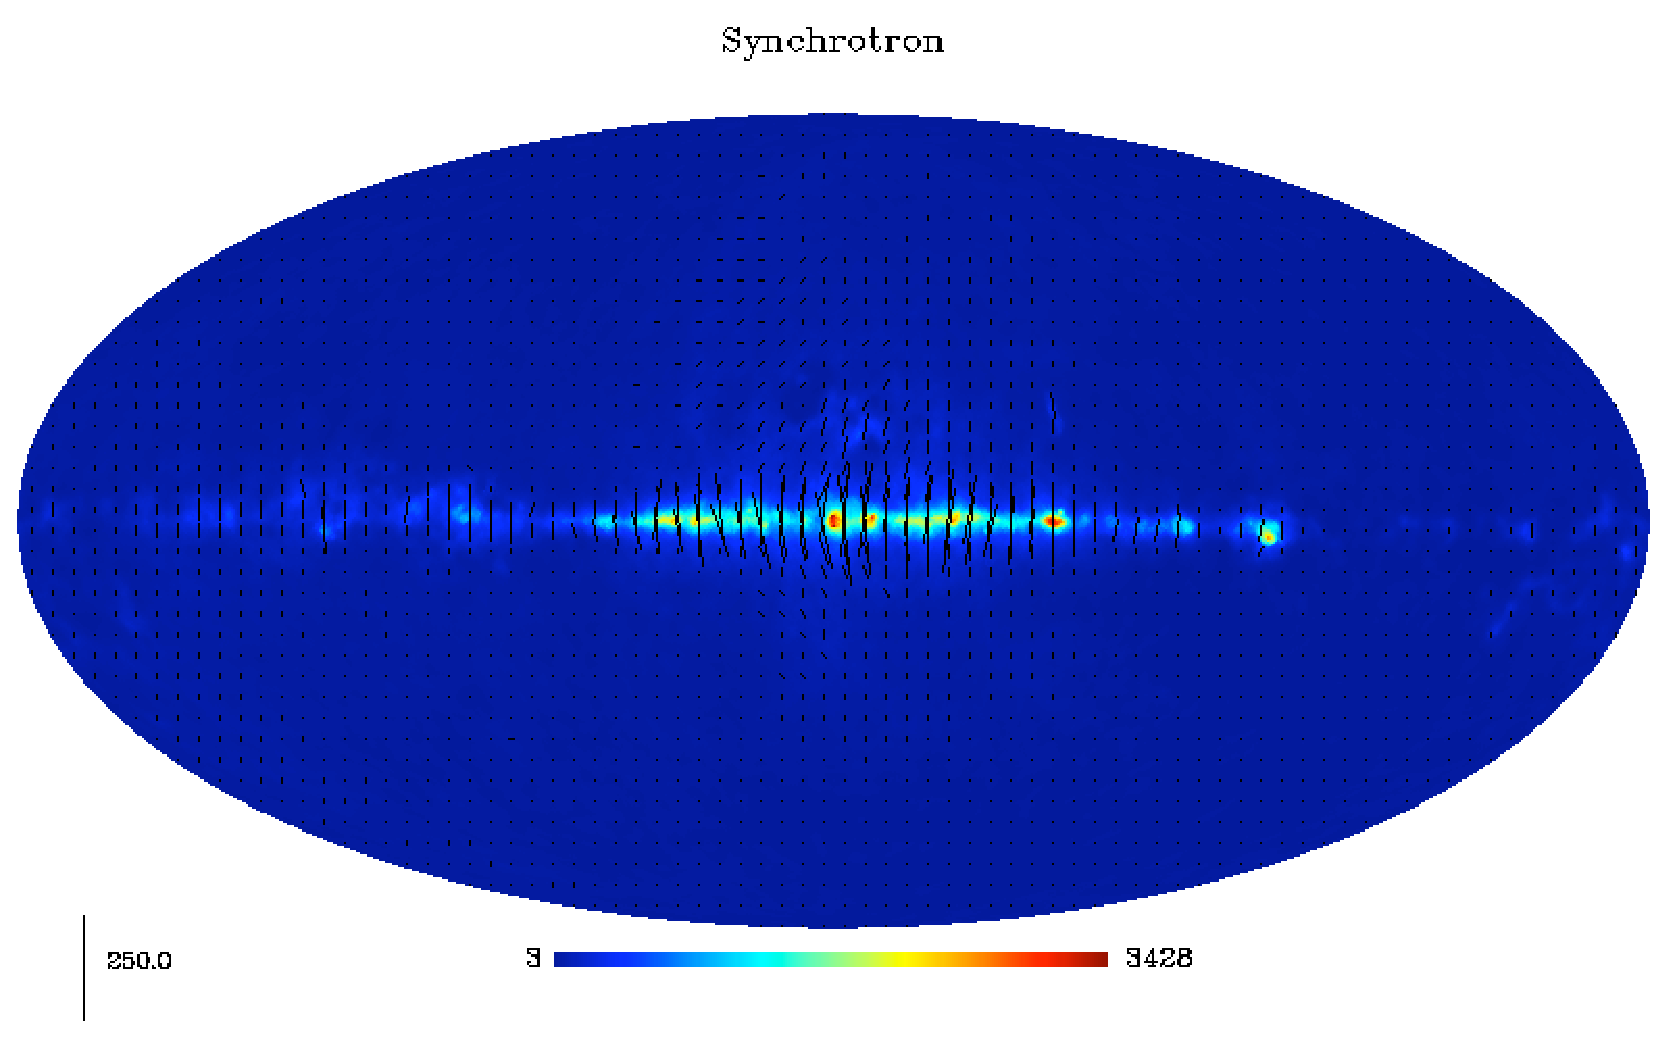
\includegraphics[width=7cm]{fig_mol_synchrotron.pdf}
 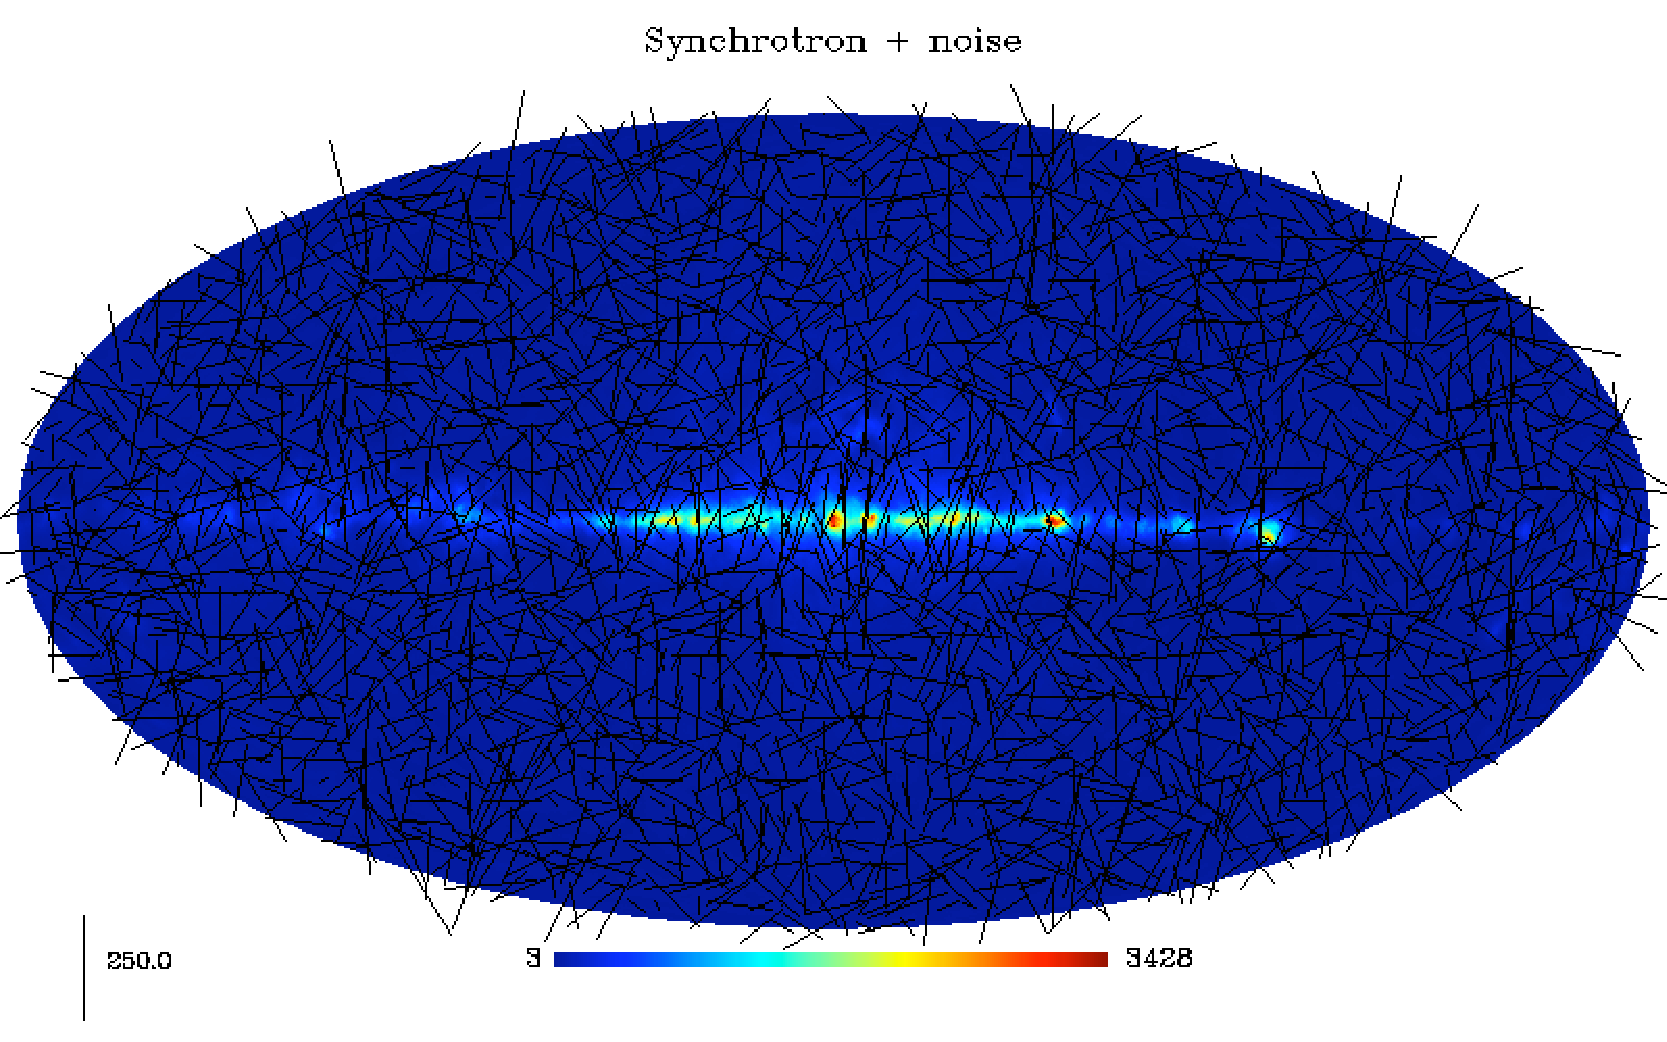
\includegraphics[width=7cm]{fig_mol_synchrotron_noise.pdf}
 }
 }
 \centerline{
 \hbox{
 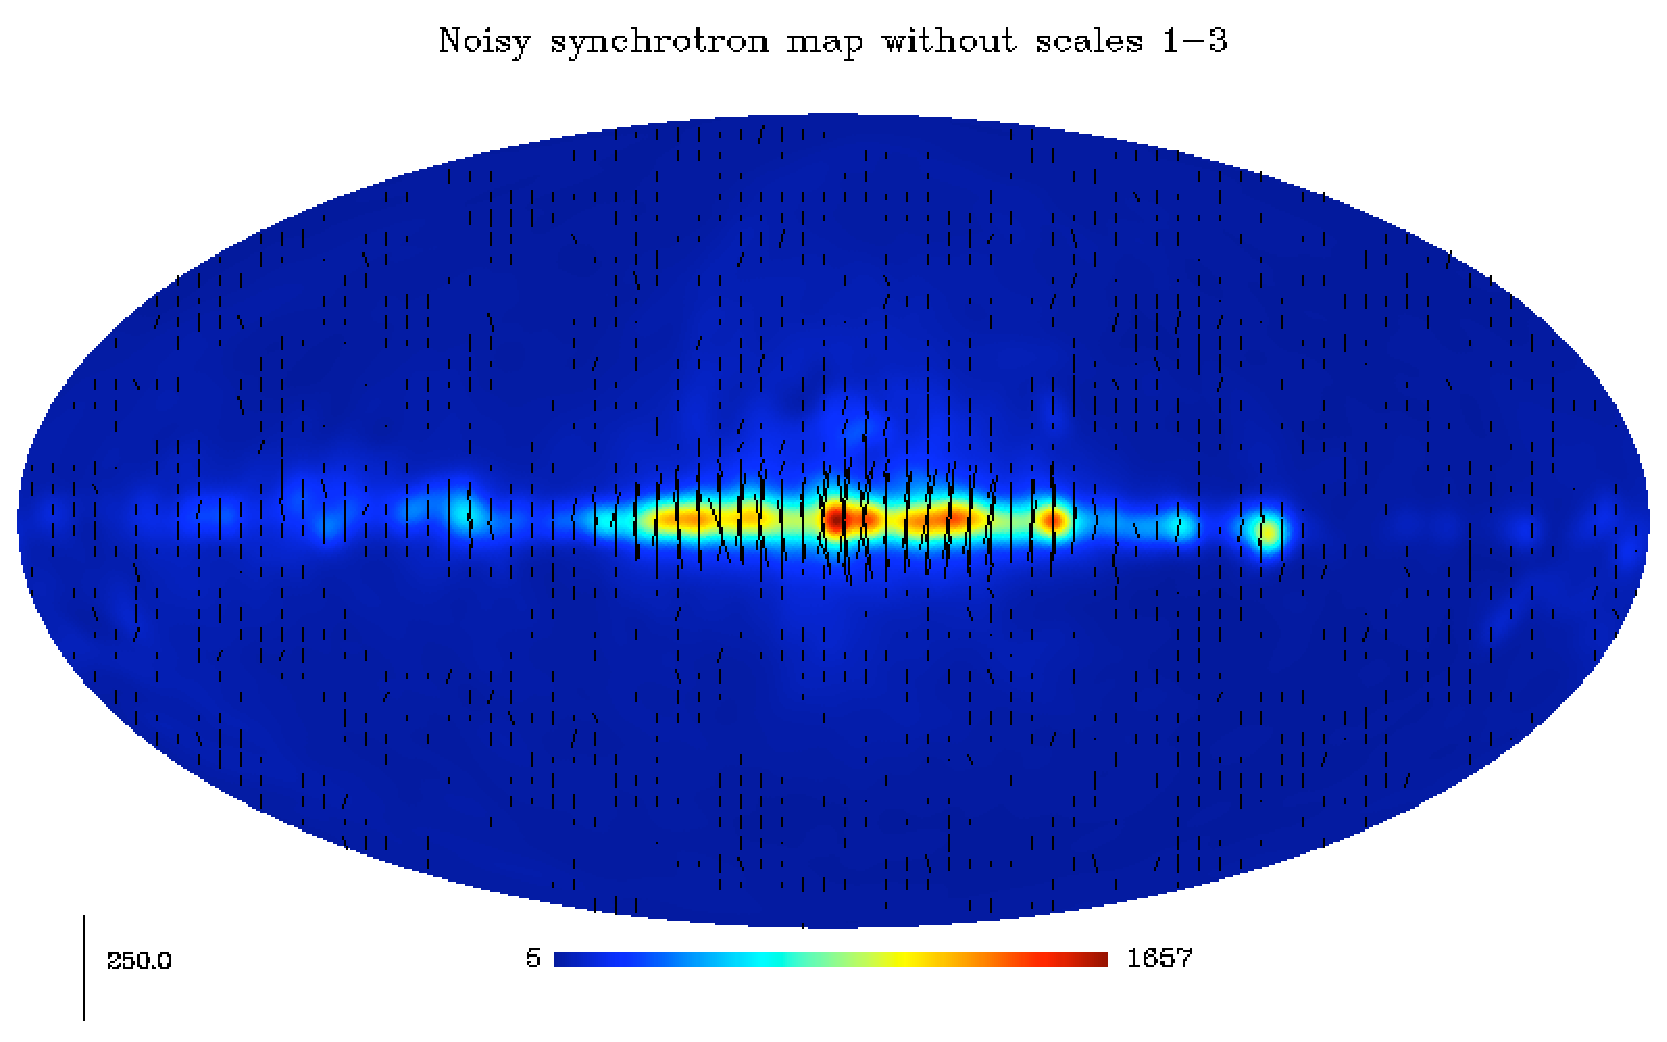
\includegraphics[width=7cm]{fig_mol_synchrotron_noise_no_scale1-3.pdf}
 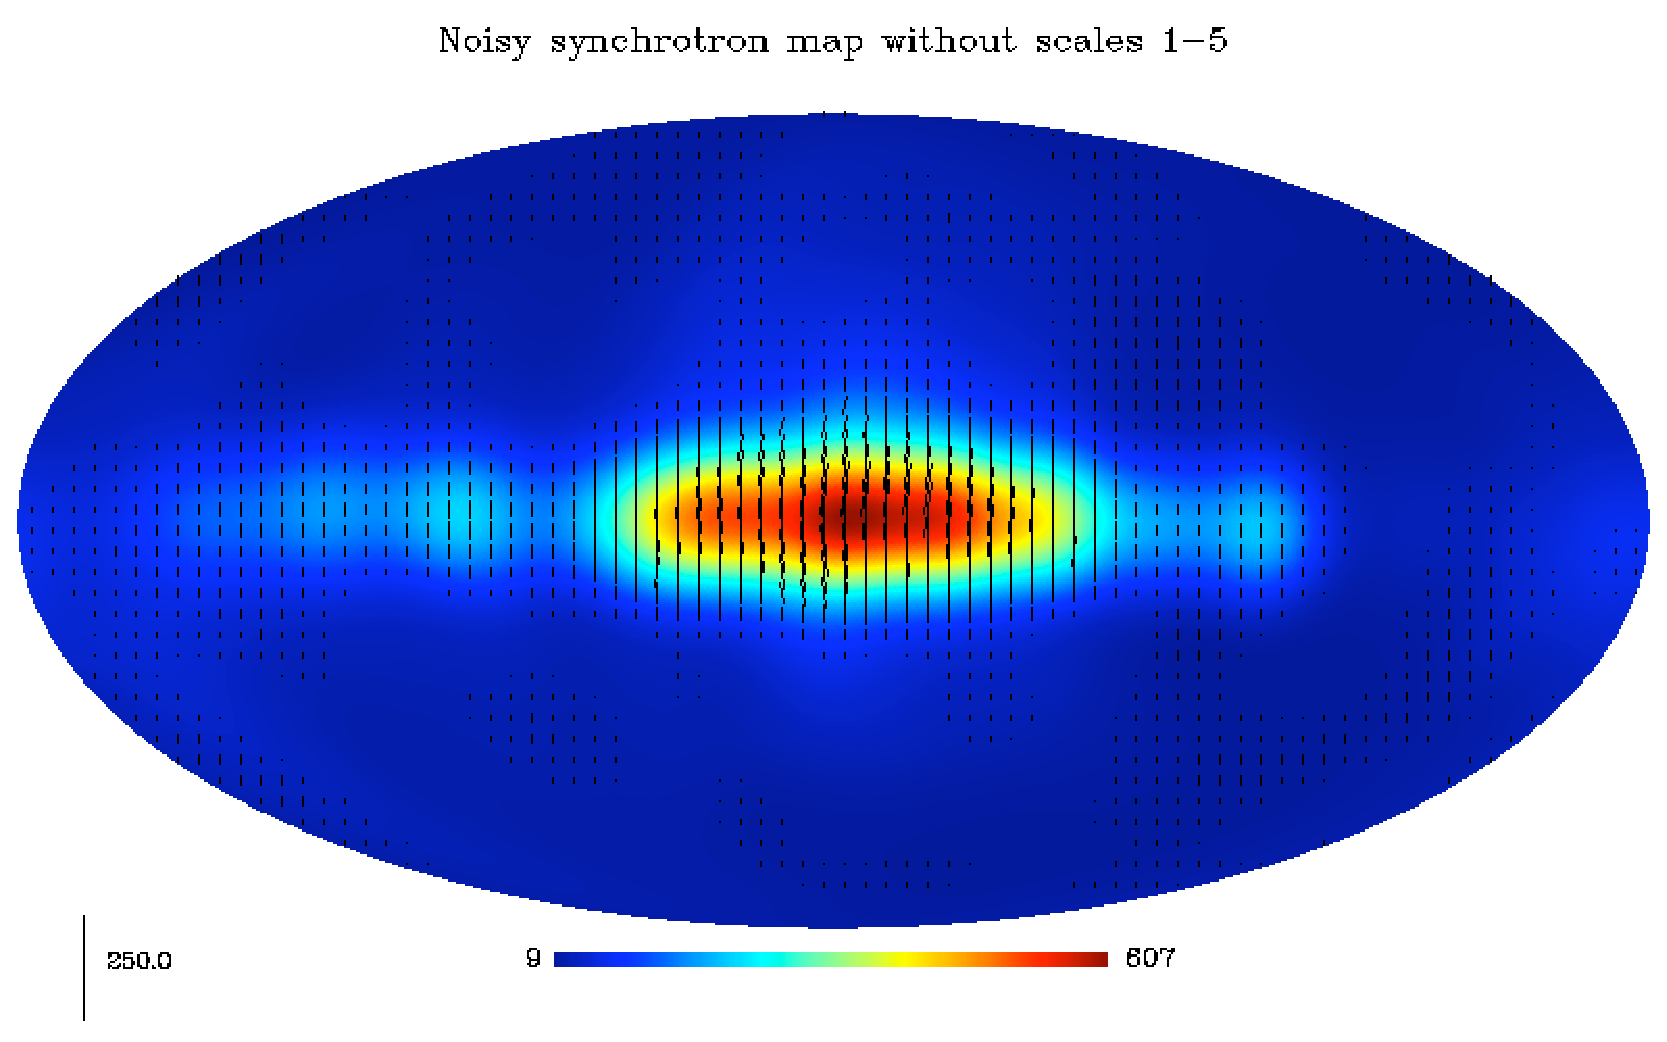
\includegraphics[width=7cm]{fig_mol_synchrotron_noise_no_scale1-5.pdf}
 }
 }
 }
\caption{ Polarized field smoothing - \textit{top left~:} simulated synchroton emission.  \textit{top right~:} same field corrupted by additive noise.
 \textit{bottom left~:} MP-multiscale reconstruction after setting to zero all coefficients from the three first scales.
\textit{bottom right~:} MP-multiscale reconstruction after setting to zero all coefficients from  the five first scales.}
\label{fig_modphase_smoothfield}
\end{figure*}
Fig.~\ref{fig_modphase_smoothfield} top  shows a simulated polarized field of the synchrotron emission and its noisy version.
We have applied the MP-multiscale transform and we remove the first three scales (i.e. we put all coefficients to zero) before 
reconstructing. The resulting image is shown on the bottom left of Fig.~\ref{fig_modphase_smoothfield}. The bottom right of 
Fig.~\ref{fig_modphase_smoothfield} corresponds to the same experiment, but by removing the five first scales. We can see that 
the field is smoother and smoother, but respecting the large scale structure of the field. This transform will be very well suited 
to CMB studies where the phase is analyzed independently of the modulus, such as in~\cite{coles05,naselsky05}.

%---------------------------------------------------------------------------------------------------------------------------------------
%---------------------------------------------------------------------------------------------------------------------------------------


\section{Polarized Wavelet Transform using Spherical Harmonics}
\label{sec:pol_iwt}

\subsection{Isotropic Undecimated Wavelet Transform on the Sphere (UWTS) }
\label{sec:UWTS}

\begin{figure*}[htb]
\centerline{
 \hbox{
 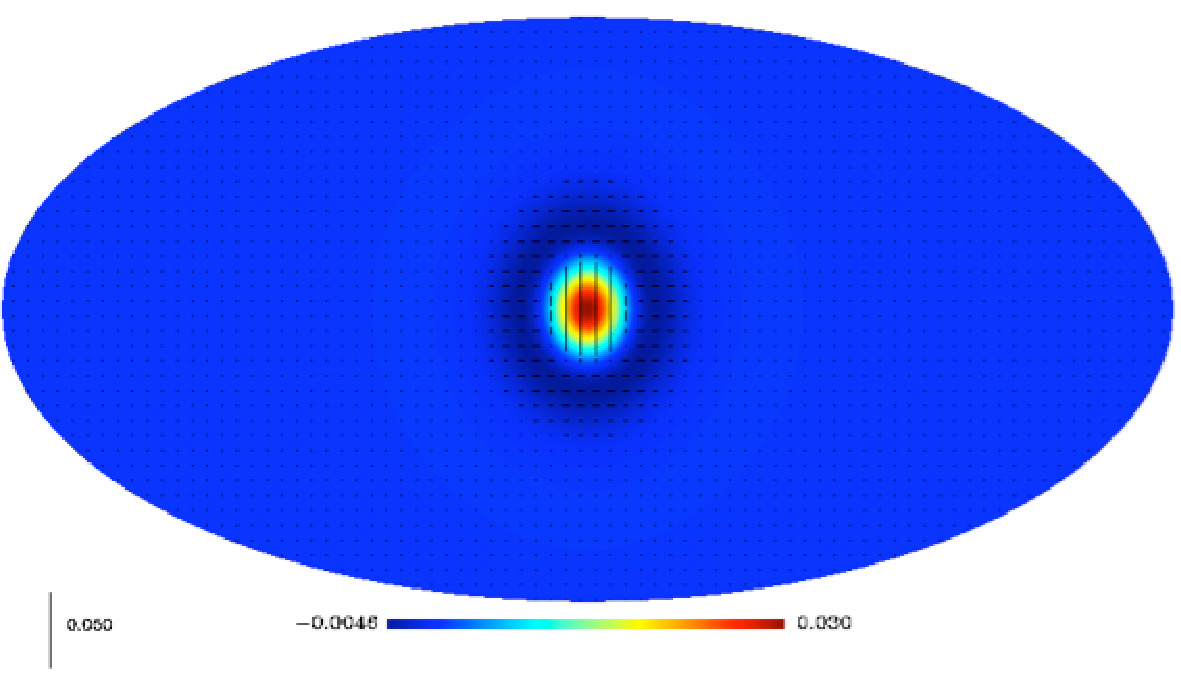
\includegraphics[width=7cm]{fig_q_iwt_back.pdf}
 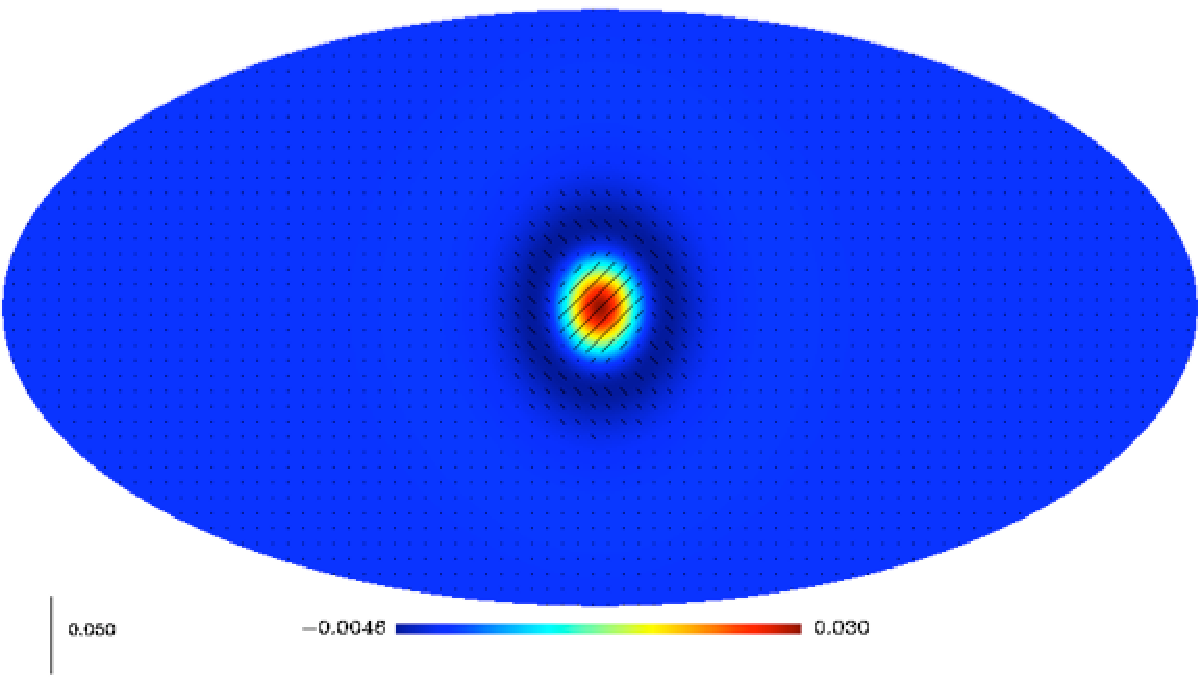
\includegraphics[width=7cm]{fig_u_iwt_back.pdf}
 }
 }
\caption{Q-isotropic wavelet transform backprojection (left) and U-isotropic wavelet backprojection (right).}
\label{fig_qu_iwt_back}
\end{figure*}


%---------------------------------------------------------------------------------------------------------------------------------------
The undecimated isotropic transform on the sphere described in~\cite{starck:sta05_2} is similar in many respects to the usual 
\emph{ \`a trous} isotropic wavelet transform. It is obtained using a zonal scaling function $\phi_{l_c}(\vartheta, \varphi)$ 
which depends only on colatitude $\vartheta$ and is invariant with respect to a change in longitude $\varphi$. It follows that 
the spherical harmonic coefficients $\hat \phi_{l_c} (l,m)$ of $\phi_{l_c}$ vanish when $m \ne 0$ which makes it simple to compute 
those spherical harmonic coefficients $\hat c_{0}(l,m)$ of $c_0 = \phi_{l_c} * f$ where $*$ stands for convolution :
\begin{eqnarray}
 \hat c_{0}(l,m) = \widehat{\phi_{l_c} * f} (l,m) = \sqrt{\frac{4\pi}{2l+1} } \hat \phi_{l_c} (l,0) \hat f(l,m) 
\end{eqnarray}
A possible scaling function~\cite{starck:book98}, defined in the spherical harmonics representation, is $\phi_{l_c}(l, m) = {2 \over 3} B_{3} ( { {2 l} \over {l_{c} } } )$ 
where $B_{3}$ is the cubic B-spline compactly supported over $[-2, 2]$. Denoting $\phi_{2^{-j} l_{c} }$ a rescaled version of 
$\phi_{l_{c}}$ with cut-off frequency $2^{-j} l_{c}$, a multi-resolution decomposition of $f$ on a dyadic scale is obtained recursively : 
\begin{eqnarray}
c_0   & = &  \phi_{ l_{c} }  * f    \nonumber    \\
c_j    &=&   \phi_{2^{-j}  l_{c}  }  * f  =   c_{j-1} * h_{j-1} \nonumber    \\
\end{eqnarray}
where the zonal low pass filters $h_{j}$ are defined by 
\begin{eqnarray}
 \hat{H}_{j}(l,m)  & =  &  \sqrt{\frac{4\pi}{2l+1} }  \hat h_{j}(l,m)  \nonumber \\
 &  =  & \left\{
  \begin{array}{ll}
  \frac {   \hat \phi_{\frac{l_{c}}{2^{j+1}} }(l,m)   }   {  \hat  \phi_{  \frac{l_{c}}{2^{j}} }(l,m)   } & \mbox{if }  l  < \frac{ l_{c}} {2^{j+1}} \quad \textrm{and}\quad m = 0\\
0 & \mbox{otherwise } \ 
  \end{array}
  \right.
\end{eqnarray}
The cut-off frequency is reduced by a factor of $2$ at each step so that in applications where this is useful such as compression, 
the number of samples could be reduced adequately. Using a pixelization scheme such as Healpix \cite{pixel:healpix}, this can easily 
be done by dividing by 2 the Healpix {\it nside} parameter when computing the inverse spherical harmonics transform. 
% Of course, this is only an approximate \emph{Sampling Theorem} but it proved sufficient for numerical purposes.  However, in the present isotropic undecimated transform, no downsampling is performed  and the maps have the same number of pixels on each scale. Hence the orthogonality requirement is relaxed, which provides us with a higher degree of freedom in the choice and design  of the wavelet function $\psi_{l_c}$ to be used with the scaling function $\phi_{l_c}$. 
As in the \emph{\`a trous} algorithm, the wavelet coefficients can be defined as the difference between two consecutive resolutions, 
$w_{j+1}(\vartheta, \varphi) = c_{j}(\vartheta, \varphi) - c_{j+1}(\vartheta, \varphi)$. This defines a zonal wavelet function $\psi_{l_c}$ as 
\begin{eqnarray}\label{wavelet}
\hat \psi_{\frac{l_c}{2^{j}}}(l,m) = \hat \phi_{\frac{l_c}{2^{j-1}}} (l,m)  - \hat \phi_{\frac{l_c}{2^{j}}}(l,m)
\end{eqnarray}

\begin{figure*}[htb]
\centerline{
\hbox{
 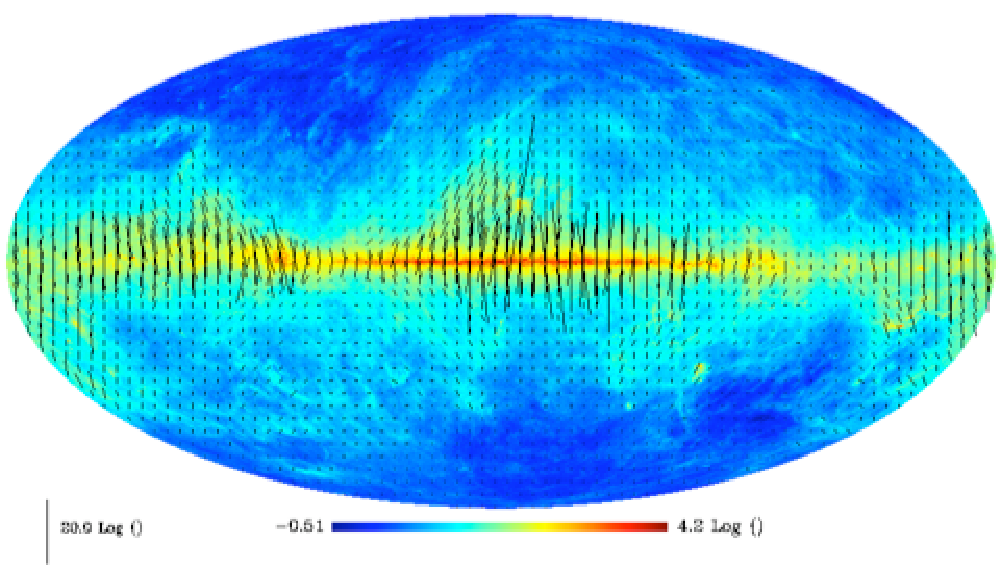
\includegraphics[width=7cm]{fig_dust_input.pdf}
}}
\caption{Simulated observations on the sphere of the polarized galactic dust emission.}
\label{fig_simu_pol_dust}
\end{figure*}

With this particular choice of wavelet function, the decomposition is readily inverted by summing the coefficient maps on all wavelet scales
 \begin{eqnarray}\label{IWT}
   %c_{0}(\vartheta, \varphi) = c_{J}(\vartheta, \varphi) + \sum_{j=1}^{J} w_j(\vartheta, \varphi)
   f(\vartheta, \varphi) = c_{J}(\vartheta, \varphi) + \sum_{j=1}^{J} w_j(\vartheta, \varphi)
\end{eqnarray}
where we have made the simplifying assumption that $f$ is equal to $c_0$. Obviously, other wavelet functions $\psi$ could be used just as well, such as the needlet function~\cite{marinucci08}.

% Also,  because of the redundancy of the described decomposition, the inverse transform  is not unique and in fact this can profitably be used to impose additional constraints on the synthesis functions (\emph{e.g.} smoothness, positivity) used in the reconstruction \cite{starck:sta06}. 

\begin{figure*}[htb]
\centerline{
\vbox{
 \hbox{
 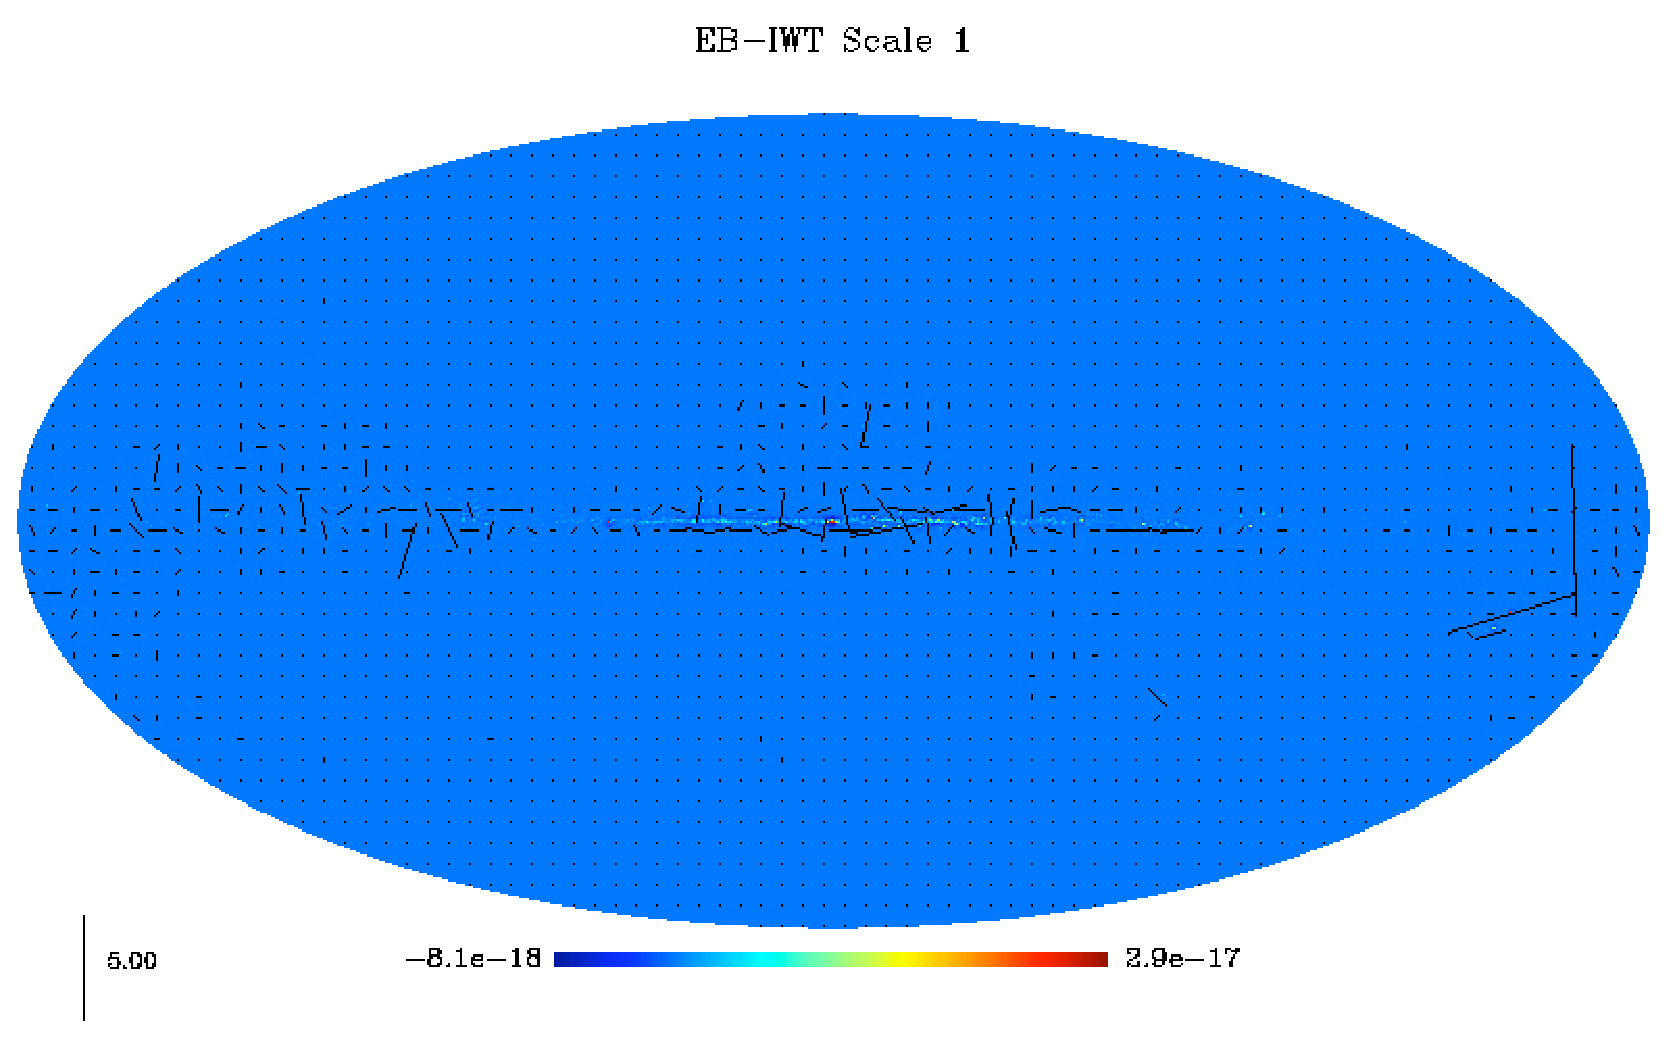
\includegraphics[width=7cm]{fig_ebiwt_scale1.pdf}
 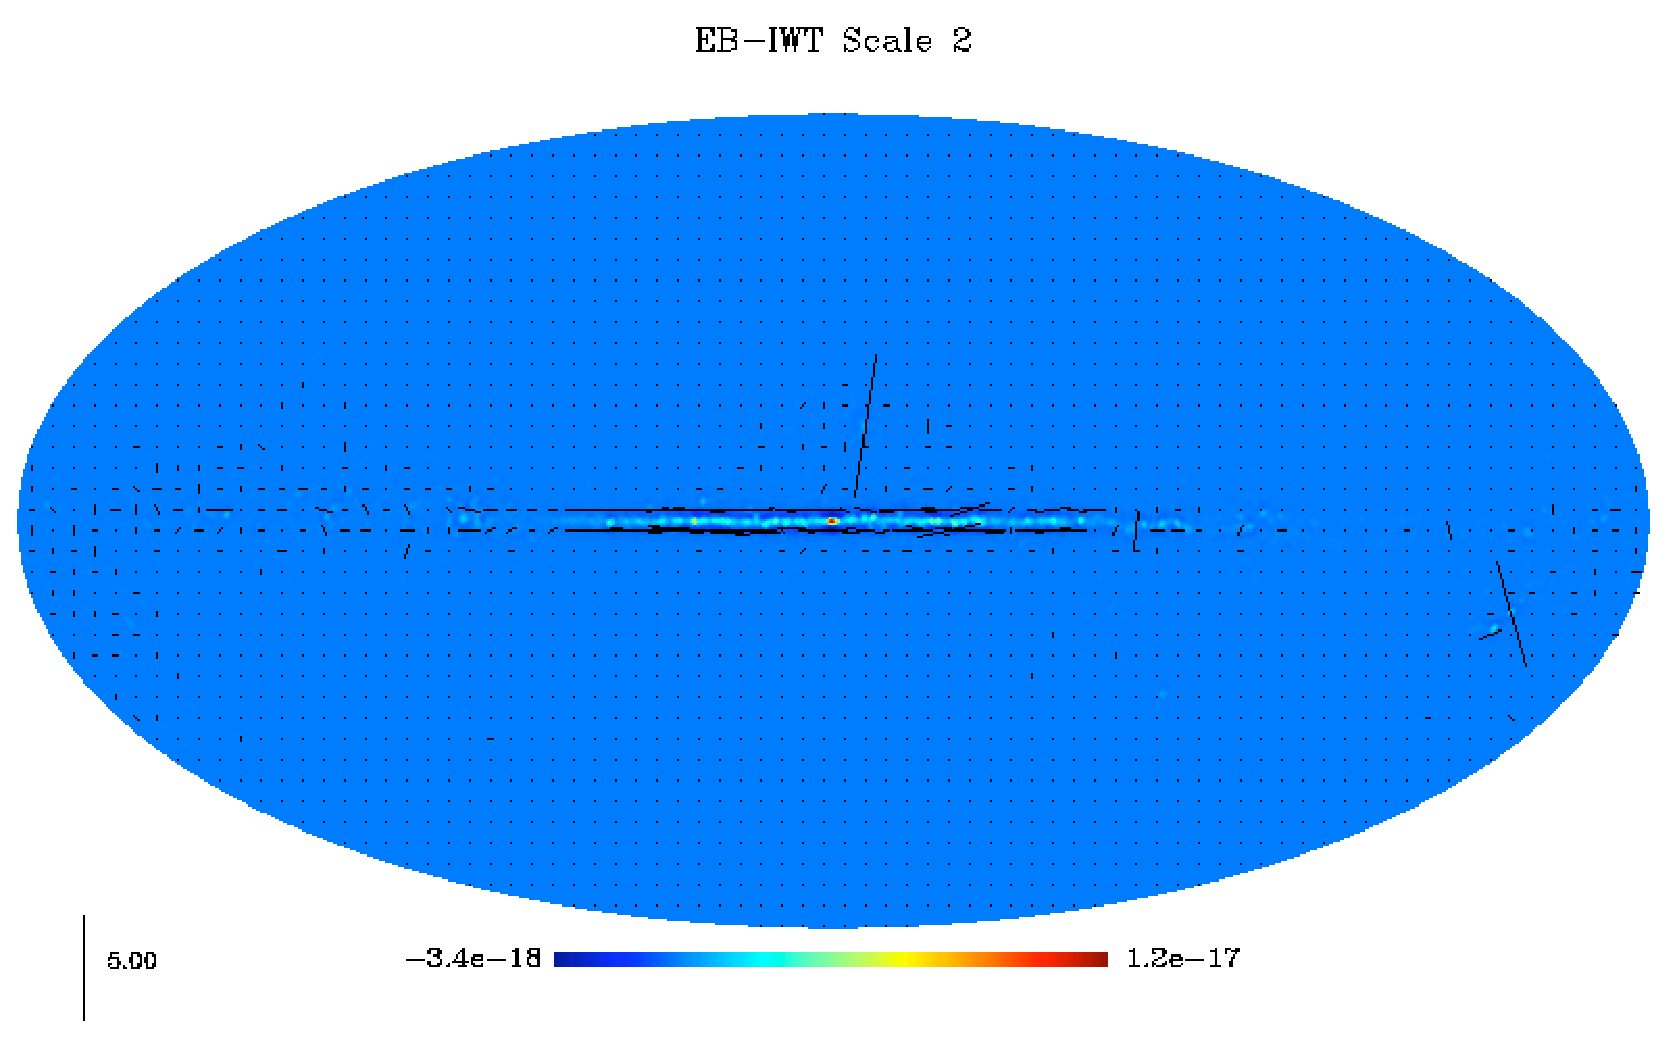
\includegraphics[width=7cm]{fig_ebiwt_scale2.pdf}
 }
 \hbox{
 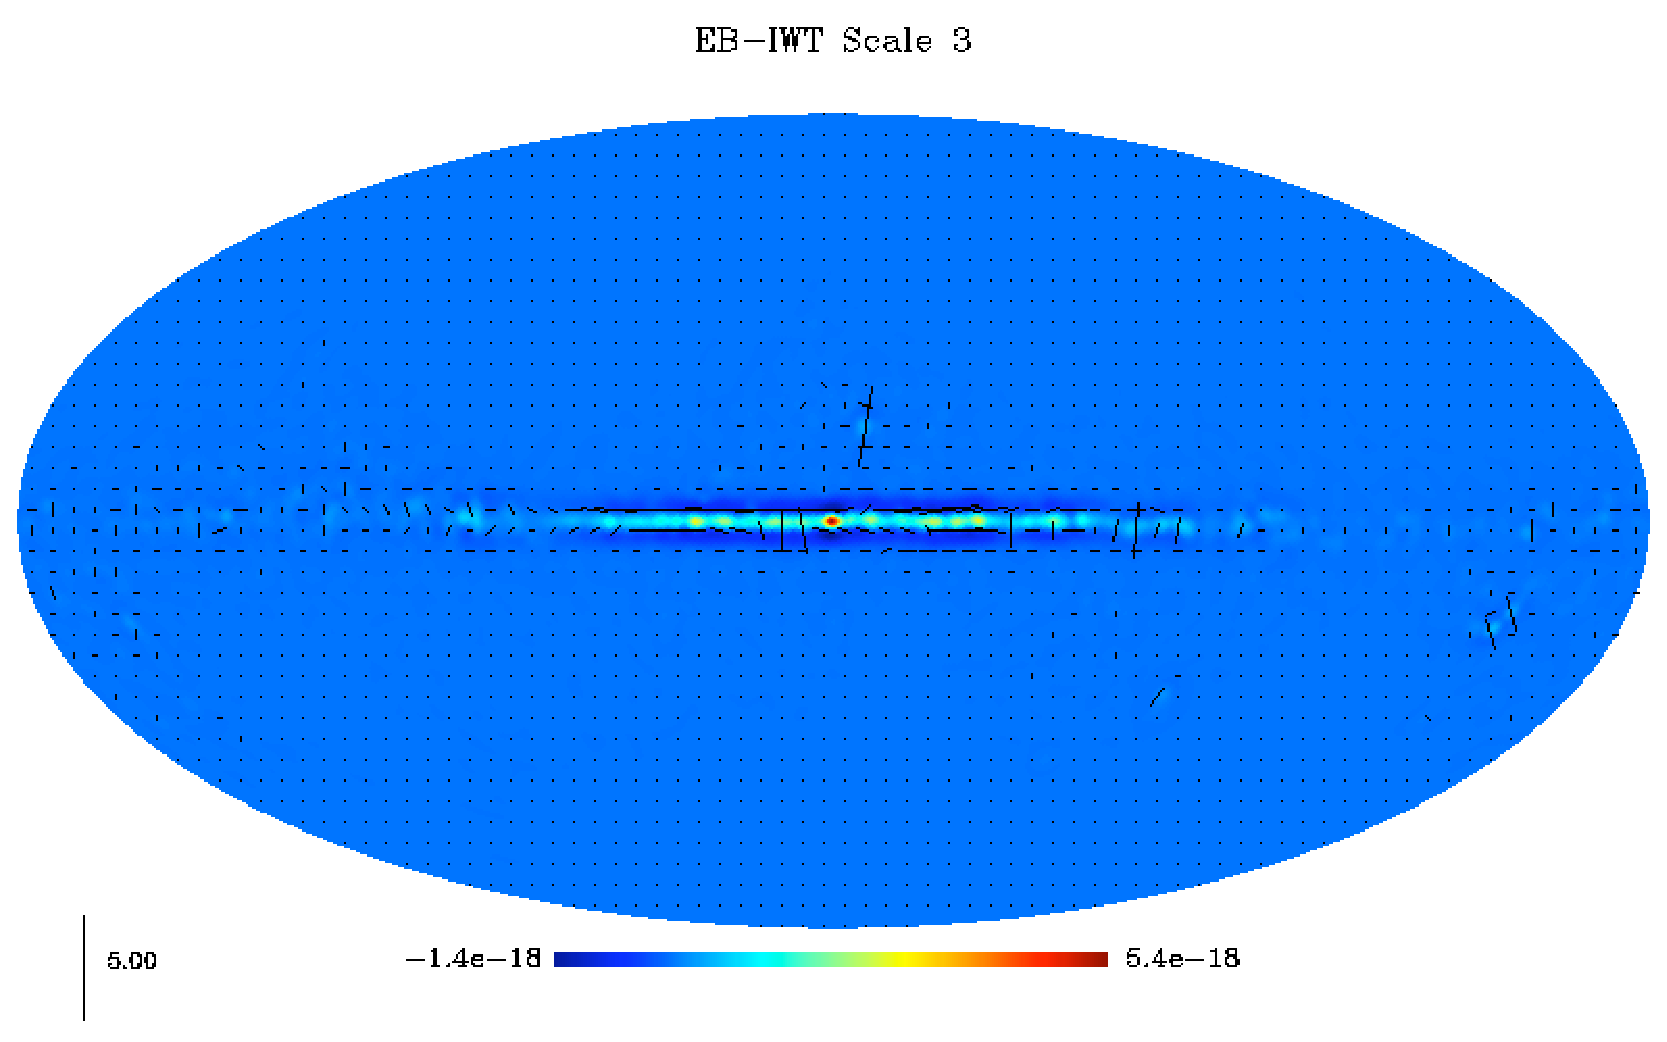
\includegraphics[width=7cm]{fig_ebiwt_scale3.pdf}
 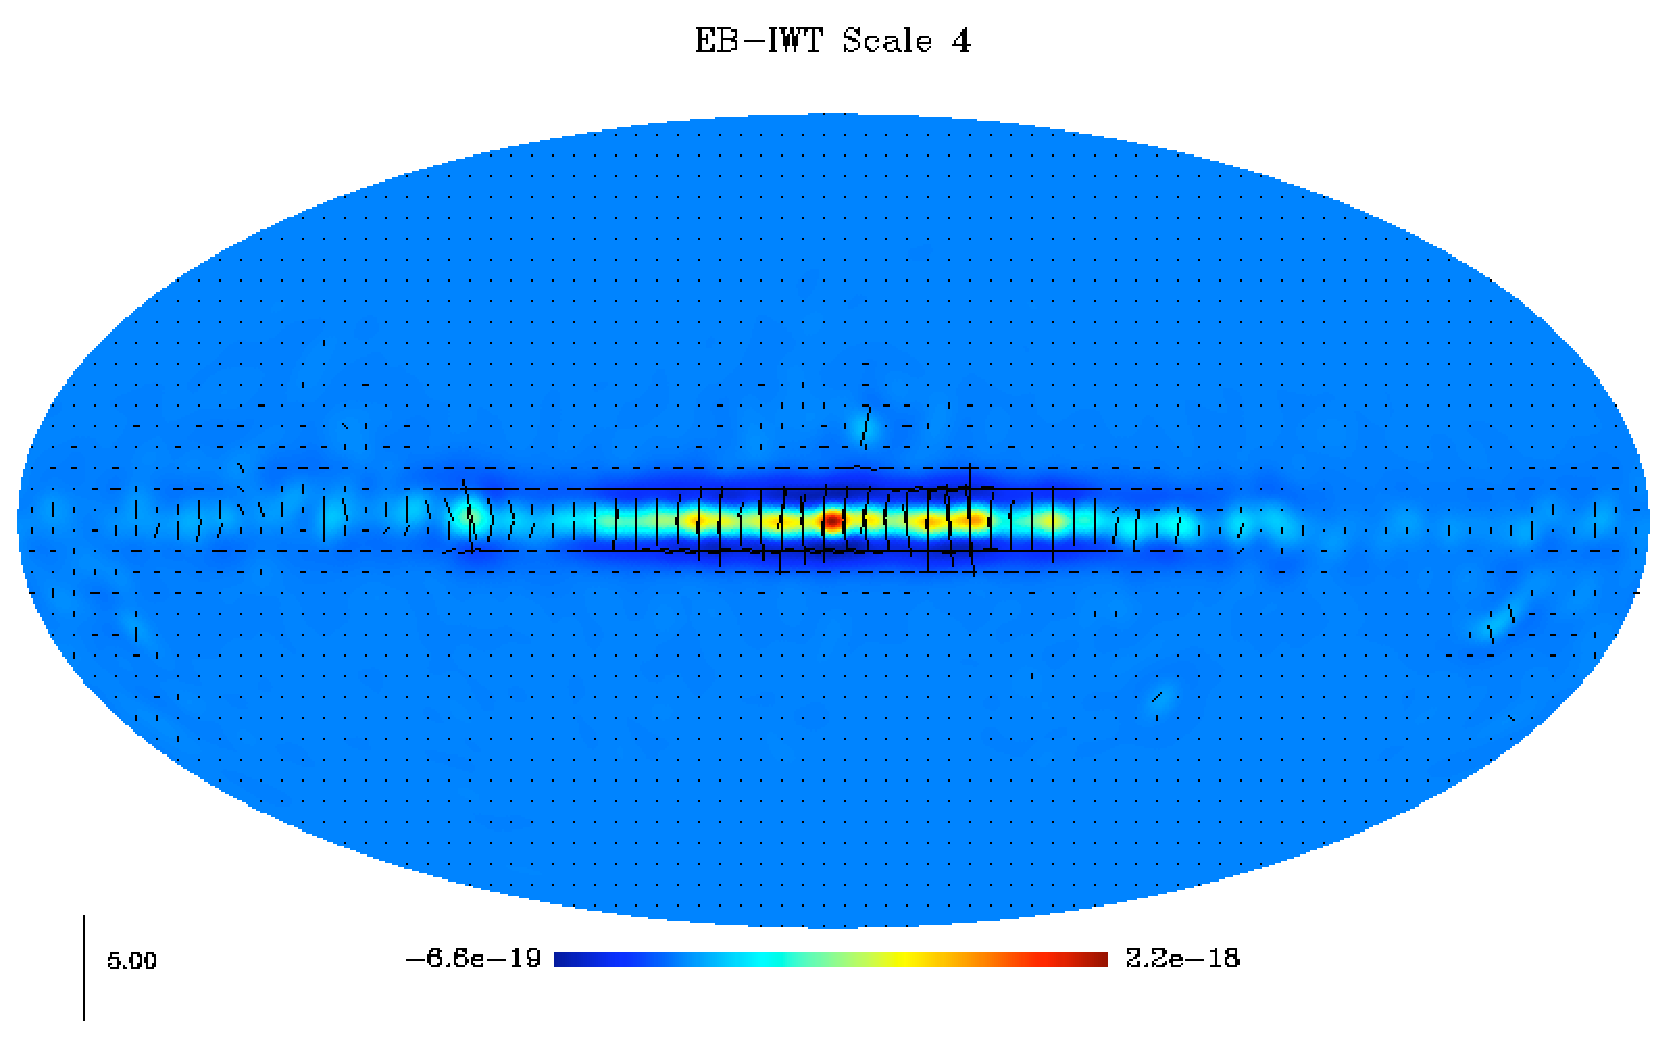
\includegraphics[width=7cm]{fig_ebiwt_scale4.pdf}
 }
  \hbox{
 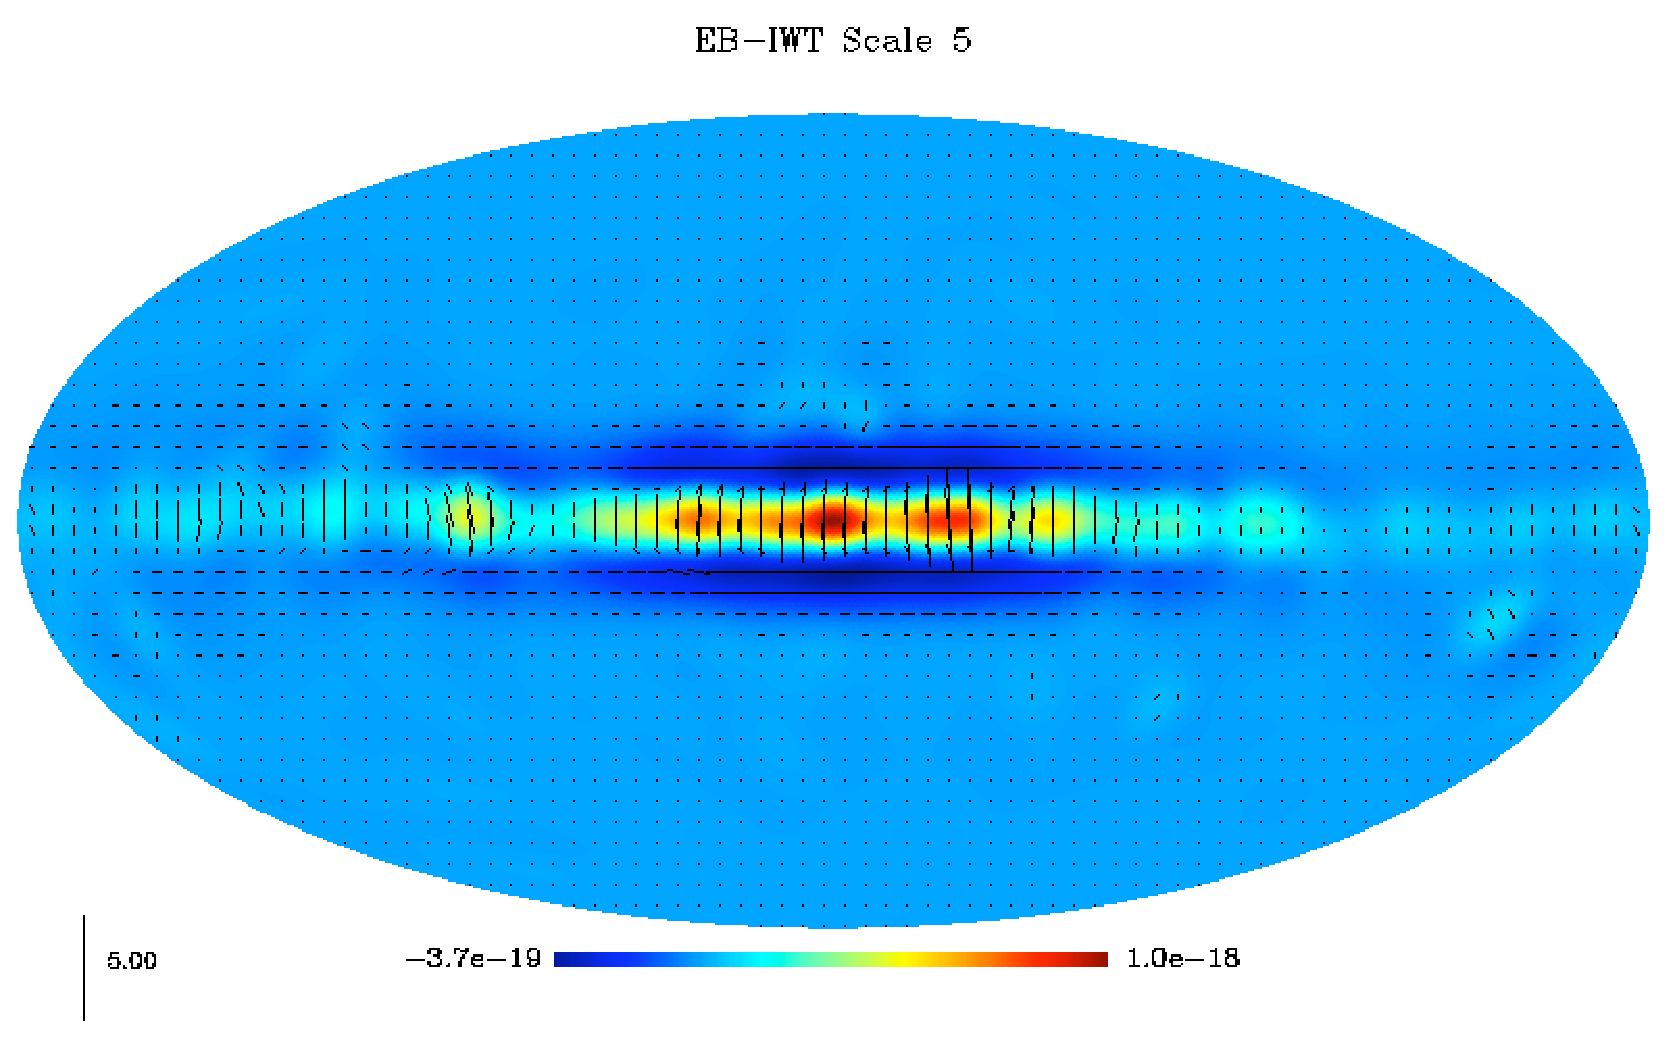
\includegraphics[width=7cm]{fig_ebiwt_scale5.pdf}
 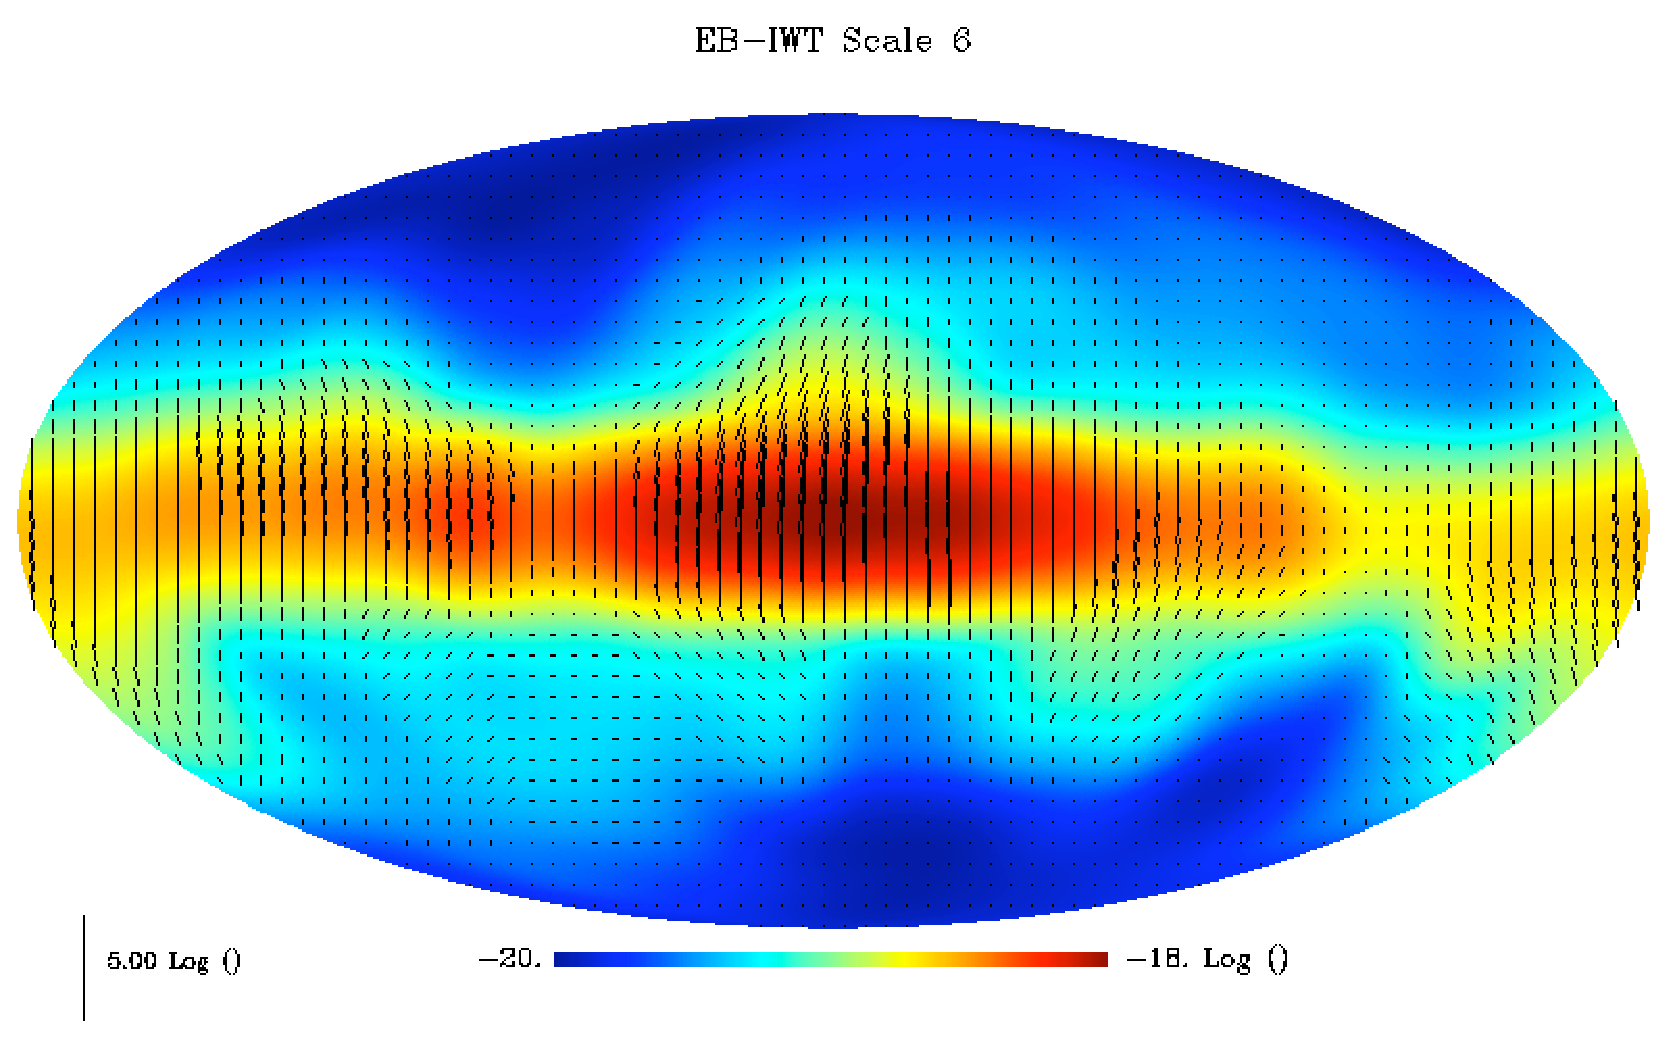
\includegraphics[width=7cm]{fig_ebiwt_scale6.pdf}
 }
  }
 }
\caption{QU-Undecimated Wavelet Transform of the simulated polarized map of galactic dust emission shown in figure~(\ref{fig_simu_pol_dust}).}
\label{fig_quwt_trans_dust}
\end{figure*}

\subsection{Extension to Polarized Data}
By applying the above scalar isotropic wavelet transform to each component $T$, $Q$, $U$ of a polarized map on the sphere, we have~:
\begin{eqnarray}
\label{tqu_iwt}
T(\vartheta, \varphi) & = c_{J}^T (\vartheta, \varphi)+ \sum_{j=1}^{J} w_j^T  (\vartheta, \varphi)\\ \nonumber
Q(\vartheta, \varphi) & = c_{J}^Q (\vartheta, \varphi)+ \sum_{j=1}^{J} w_j^Q (\vartheta, \varphi)\\ \nonumber
U(\vartheta, \varphi) & = c_{J}^U (\vartheta, \varphi)+ \sum_{j=1}^{J} w_j^U (\vartheta, \varphi)
\end{eqnarray}
where $c_{J}^X$ stands for the low resolution approximation to component $X$ and $w_j^X$ is the map of wavelet coefficients of that component on scale $j$. This leads to the following decomposition~:
\begin{eqnarray}
(Q \pm iU)[k] =    (c^Q_{J} \pm c^U_{J,p})[k]   +   \sum_{j=1}^J   ( w_{j}^Q \pm w_{j}^U )[k]
\label{eq_qu_rec_uwt}
\end{eqnarray}
Fig.\ref{fig_qu_iwt_back} shows the backprojection of a Q-wavelet coefficient (left) and a $U$-wavelet coefficient (right).
Fig.~\ref{fig_quwt_trans_dust} shows the undecimated isotropic polarized wavelet transform of the dust image shown on 
Fig.~\ref{fig_simu_pol_dust} using six scales, \textit{i.e.} five wavelet scales and the coarse approximation.
%---------------------------------------------------------------------------------------------------------------------------------------
%---------------------------------------------------------------------------------------------------------------------------------------
\section{Polarized Curvelet Transform}
\label{sec:pol_cur}
% \begin{figure*}
% \centerline{
% \hbox{
% \psfig{figure=fig_back_cur_sphere.ps,bbllx=1cm,bblly=7cm,bburx=20cm,bbury=20cm,height=8.5cm,width=12cm,clip=}
% }}
% \caption{Backprojection of  various curvelet coefficients at different scales and orientations on the sphere.  Each map is obtained by setting all but one of the curvelet coefficients to zero, and applying an inverse curvelet transform. Depending on the scale and the position of the non zero curvelet coefficient, the reconstructed image presents a feature with a given width, length and orientation.}
 %\label{Figure:back_cur}
% \end{figure*}
 \begin{figure*}[htb]
\centerline{
\vbox{
 \hbox{
 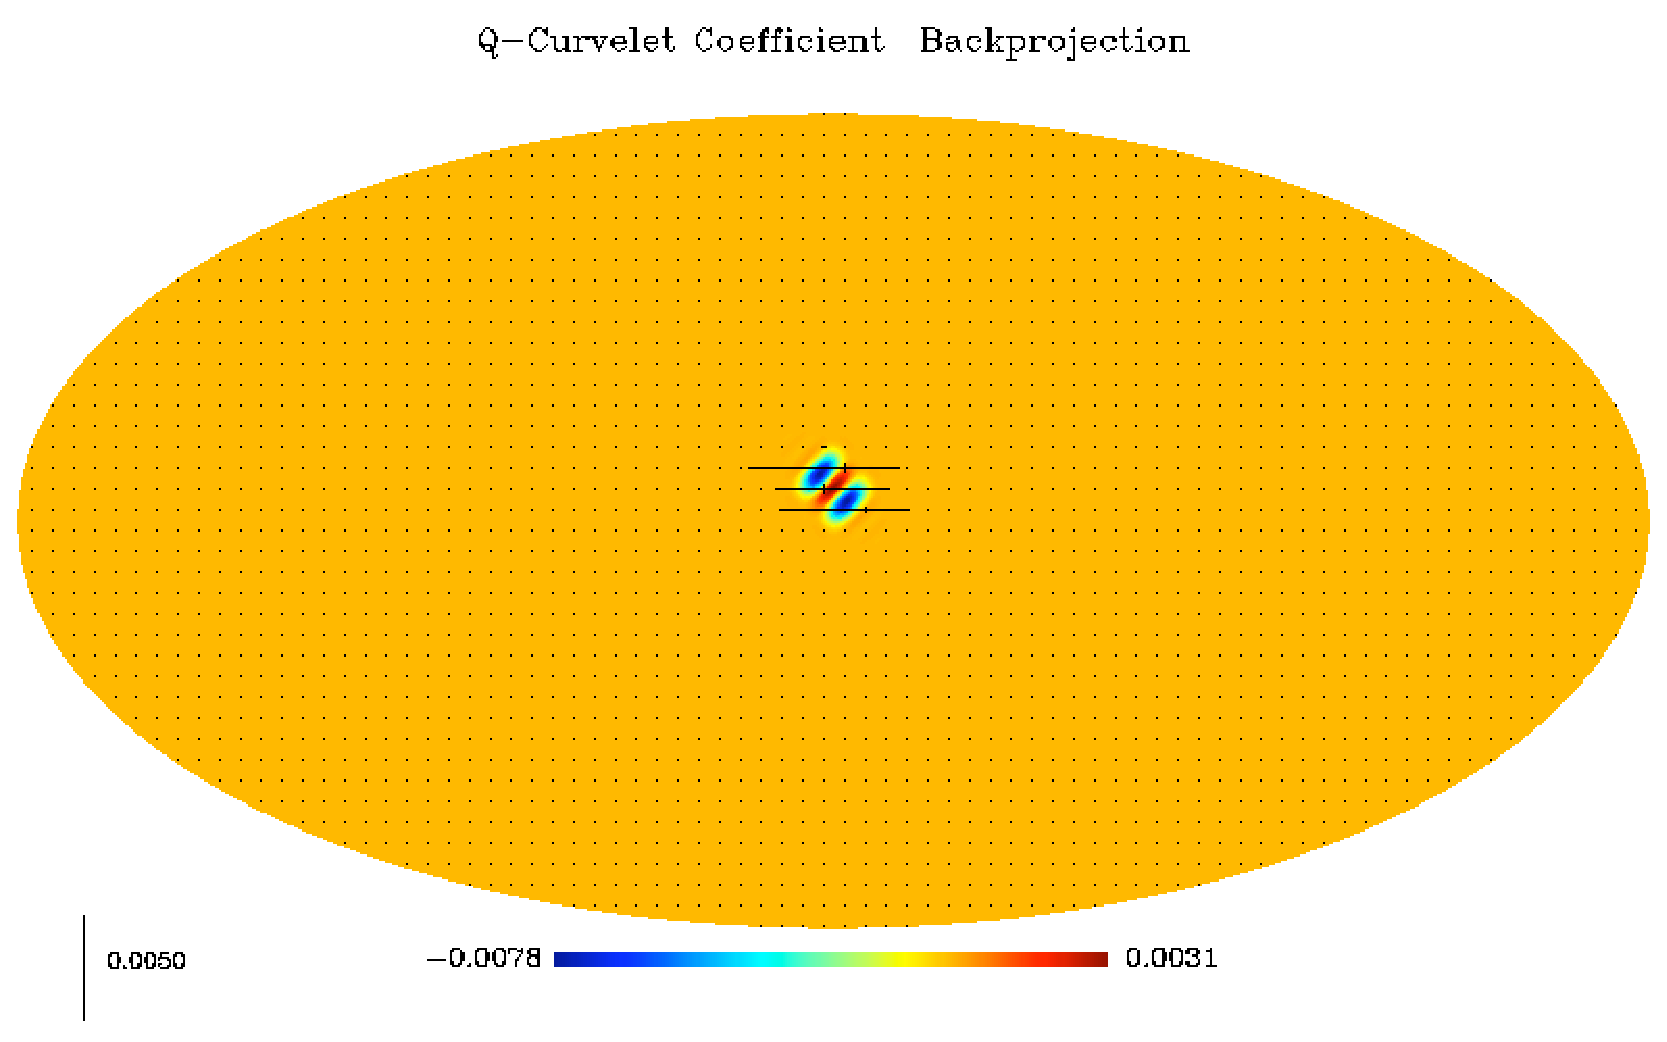
\includegraphics[width=7cm]{fig_mol_backproj_qucur_qj3.pdf}
 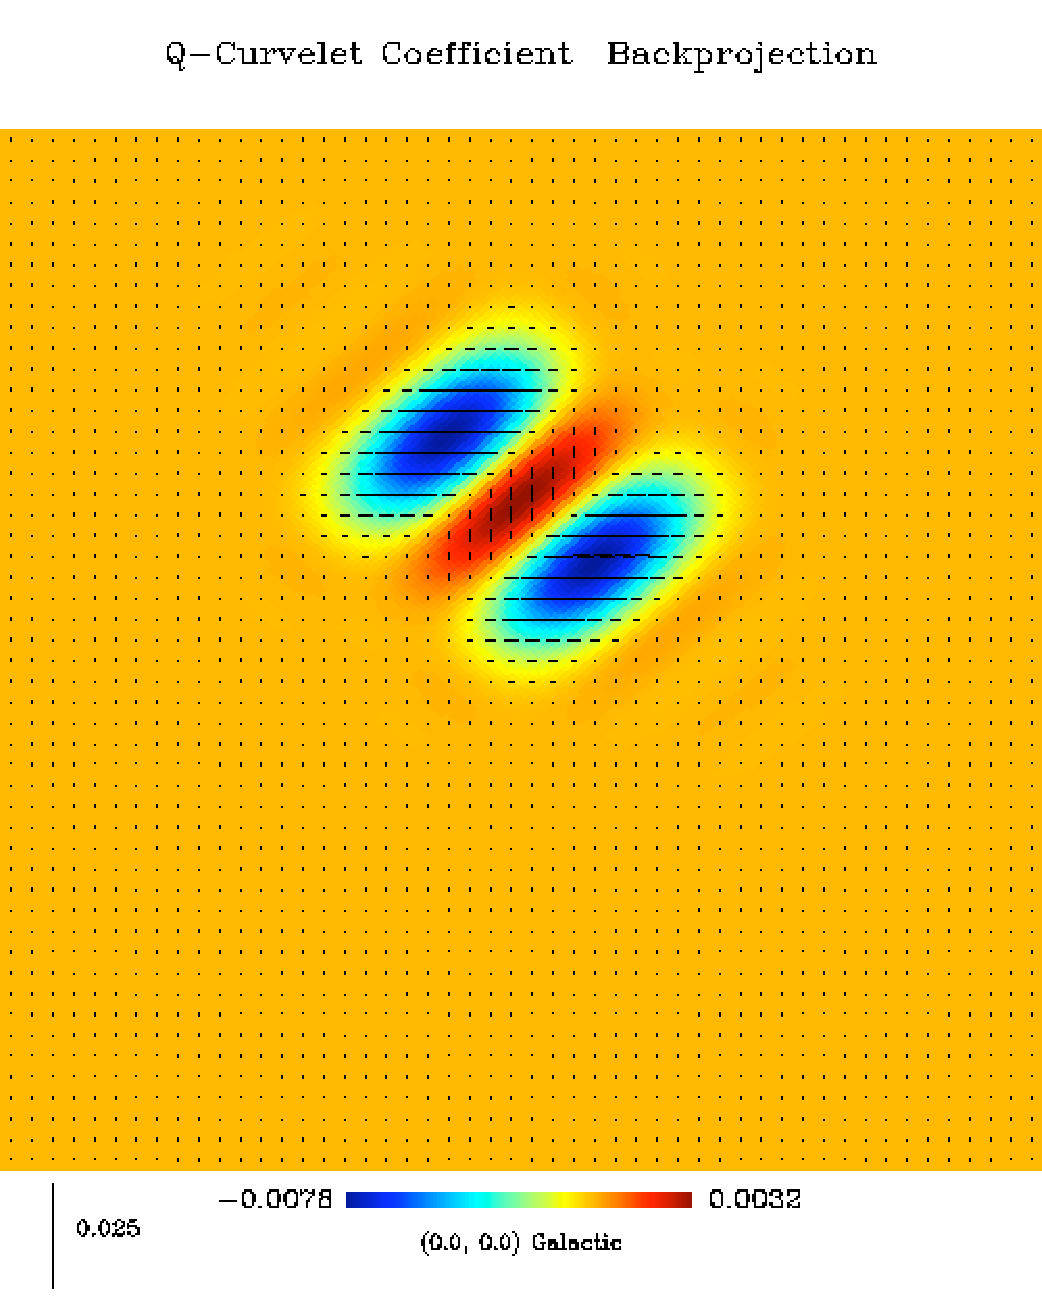
\includegraphics[width=4cm]{fig_backproj_qucur_qj3.pdf}
 }
 \hbox{
 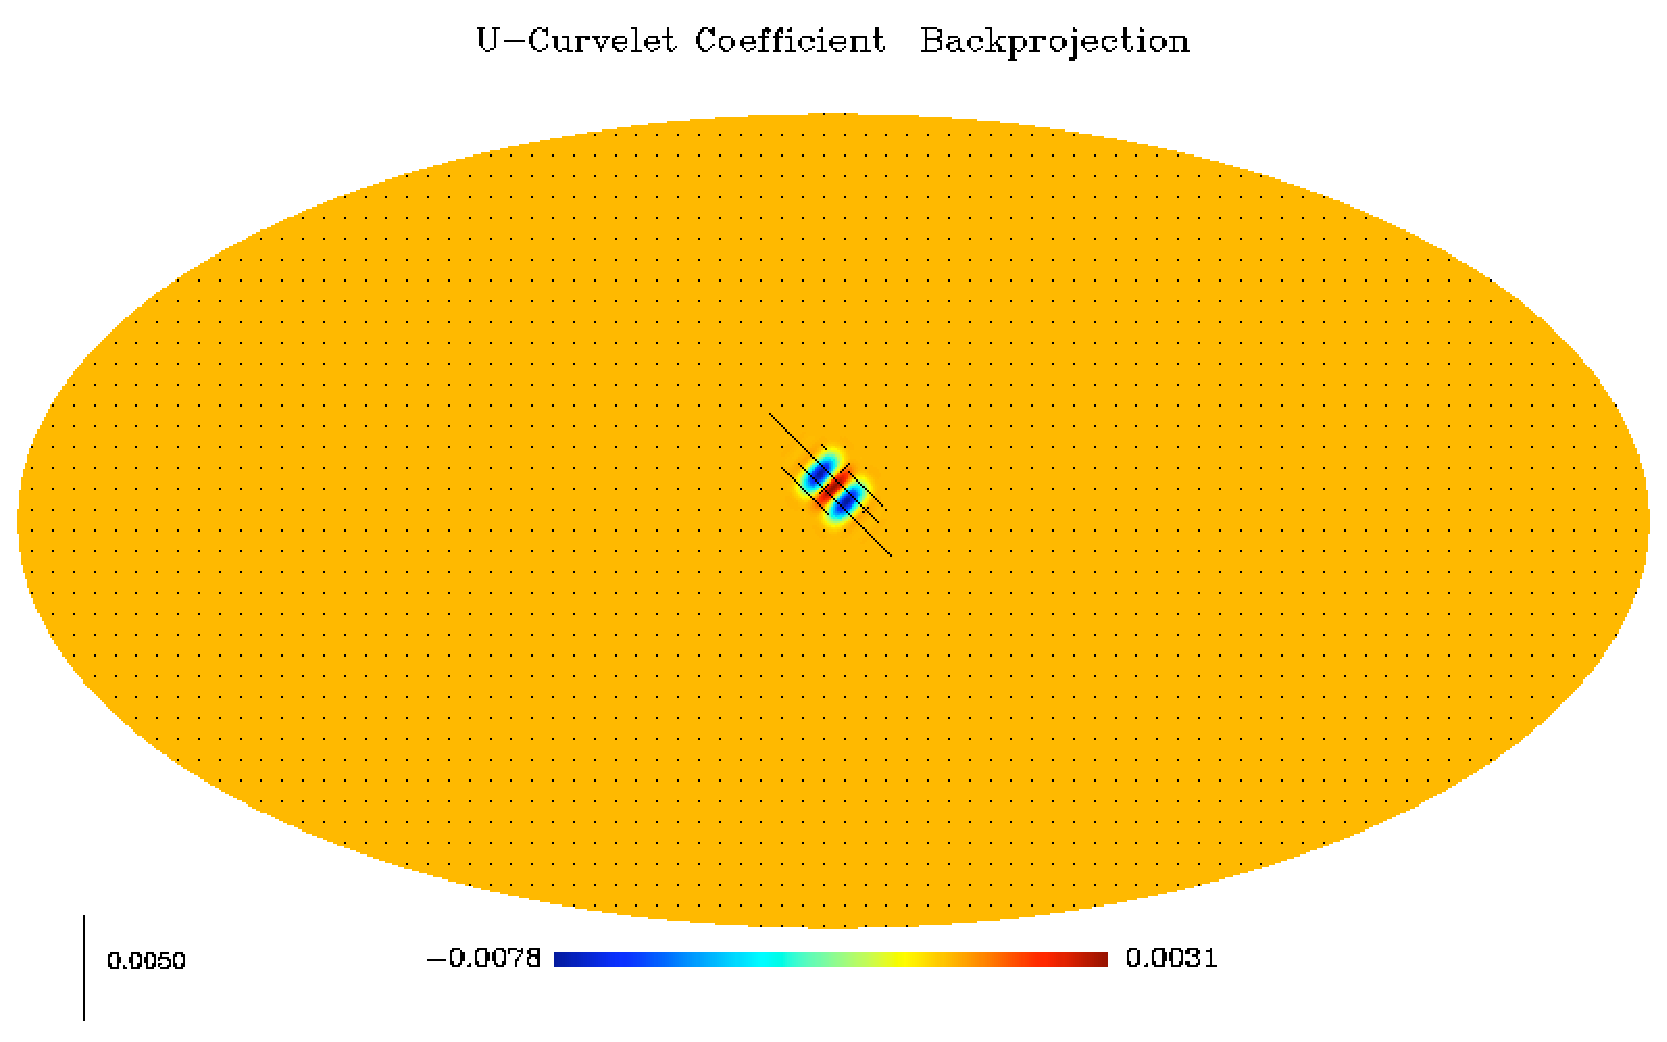
\includegraphics[width=7cm]{fig_mol_backproj_qucur_uj3.pdf}
 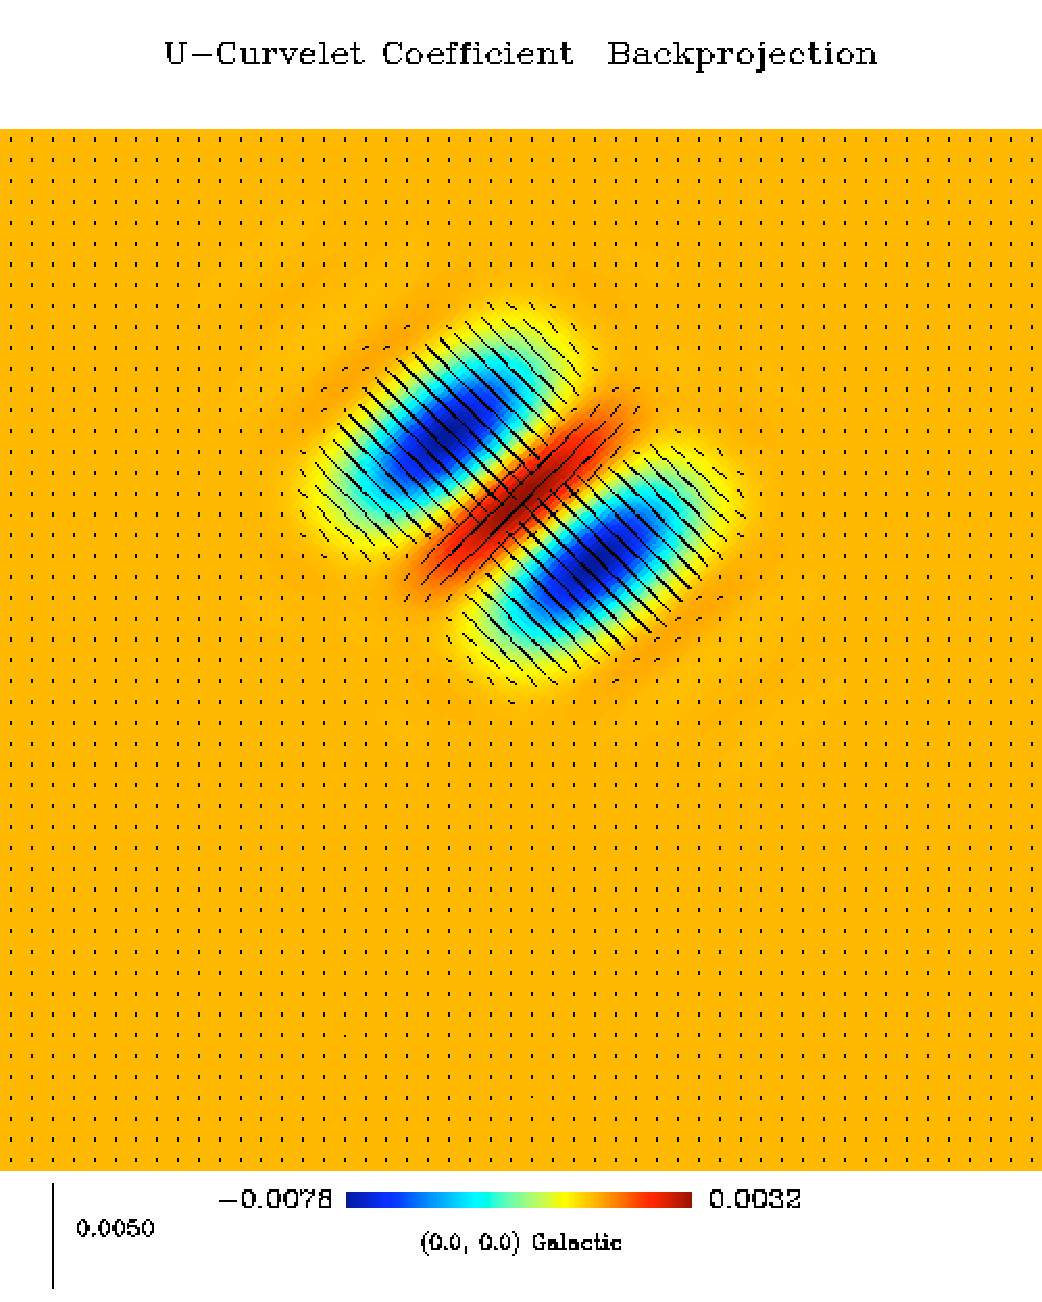
\includegraphics[width=4cm]{fig_backproj_qucur_uj3.pdf}
 }
  }
 }
\caption{Top, Q-curvelet backprojection (left)  and zoom (right). Bottom, U-curvelet backprojection (left)  and zoom. }
\label{fig_qucur_back}
\end{figure*}
The 2D ridgelet transform \cite{cur:candes99_1} was developed in an attempt to overcome some limitations inherent in former multiscale methods 
\emph{e.g.} the 2D wavelet, when handling smooth images with edges \textit{i.e.} singularities along smooth curves. Ridgelets are translation 
invariant \emph{ridge} functions with a wavelet profile in the normal direction. Although ridgelets provide sparse representations of smooth 
images with straight edges, they fail to efficiently handle edges along curved lines. This is the framework for curvelets which were given a 
first mathematical description in \cite{Curvelets-StMalo}. Basically, the curvelet dictionary is a multiscale pyramid of localized directional 
functions with anisotropic support obeying a specific parabolic scaling such that at scale $2^{-j}$, its length is $2^{-j/2}$ and its width is $2^{-j}$. 
This is motivated by the parabolic scaling property of smooth curves. Other properties of the curvelet transform as well as decisive optimality results 
in approximation theory are reported in \cite{Curvelets-StMalo,CandesDonohoCurvelets}. Notably, curvelets provide optimally sparse representations 
of manifolds which are smooth away from edge singularities along smooth curves. Several digital curvelet transforms \cite{cur:donoho99,starck:sta01_3,cur:demanet06} 
have been proposed which attempt to preserve the essential properties of the continuous curvelet transform and many papers \cite{starck:sta04,felix2008,starck:sta04} 
report on their successful application in image processing experiments. The so-called first generation discrete curvelet described in \cite{cur:donoho99,starck:sta01_3} 
consists in applying the ridgelet transform to sub-images of a wavelet decomposition of the original image. By construction, the sub-images are 
well localized in space and frequency and the subsequent ridgelet transform provides the necessary directional sensitivity. This latter implementation 
in combination with the good geometric properties of the Healpix pixelization scheme, inspired the digital curvelet transform on the sphere~\cite{starck:sta05_2}. 
The digital curvelet transform on the sphere is clearly invertible in the sense that each step of the overall transform is itself invertible. 
The curvelet transform on the sphere has a redundancy factor of $16J + 1$ when $J$ scales are used, which may be a problem for handling huge data sets 
such as from the future Planck-Surveyor experiment. This can be reduced by substituting the pyramidal wavelet transform to the undecimated wavelet 
transform in the above algorithm. More details on the wavelet, ridgelet, curvelet algorithms on the sphere can be found in \cite{starck:sta05_2}. 
As for the isotropic wavelet on the sphere, a straightforward extension to polarized data will consist in applying successively the curvelet transform 
on the sphere to the three components $T$, $Q$ and $U$. Figure~\ref{fig_qucur_back} shows the backprojection of a Q-curvelet coefficient and 
U-curvelet coefficient. Clearly, the shapes of these polarized curvelet functions are very different from the polarized wavelet functions.%---------------------------------------------------------------------------------------------------------------------------------------
%---------------------------------------------------------------------------------------------------------------------------------------
\section{Polarized E/B Wavelet and E/B Curvelet}
\label{sec:pol_eb}

\subsection{Introduction}
We have seen that the generalization of the Fourier representation for polarized data on the sphere is the spin-2 spherical harmonics basis denoted $_{\pm 2}Y_{\ell m}$: 
\begin{equation} 
Q \pm i U  = \sum_{\ell, m}  { _{\pm 2}a_{\ell m}}   {_{\pm 2}Y_{\ell m} }
\end{equation} 
  
At this point, it is convenient~\cite{zalda} to introduce the two quantities denoted $E$ and $B$ which are defined on the sphere by 
\begin{eqnarray}\label{EB}
E = &  \sum_{\ell, m}   a_{\ell m} ^E Y_{\ell m} =  \sum_{\ell, m}  - \frac{ 1}{2}   ({_{ 2}a_{\ell m}}  +  {_{- 2}a_{\ell m}} )    Y_{\ell m} \\ \nonumber
B = & \sum_{\ell, m}   a_{\ell m} ^B Y_{\ell m} =  \sum_{\ell, m}  i \frac{ 1}{2}    ({_{ 2}a_{\ell m}}  -  {_{- 2}a_{\ell m}} )   Y_{\ell m} 
\end{eqnarray} 
%\begin{equation}\label{EB}
%E =  \sum_{\ell, m}   a_{\ell m} ^E Y_{\ell m} =  \sum_{\ell, m}  - \frac{   {_{ 2}a_{\ell m}}  +  {_{- 2}a_{\ell m}}  }  {2}  Y_{\ell m}  \quad \quad 
%B =  \sum_{\ell, m}   a_{\ell m} ^B Y_{\ell m} =  \sum_{\ell, m}  i \frac{   {_{ 2}a_{\ell m}}  -  {_{- 2}a_{\ell m}}  }  {2}   Y_{\ell m} 
%\end{equation} 
where $Y_{\ell m}$ stands for the usual spin 0 spherical harmonics basis functions. The quantities $E$ and $B$ are derived by applying 
the spin lowering operator twice to $Q + i U$  and the spin raising operator twice to $Q - i U$ so that $E$ and $B$ are real scalar 
fields on the sphere, invariant through rotations of the local reference frame. The normalization of $a_{\ell m} ^E$ and $a_{\ell m} ^B$ 
chosen in the latter definition is purely conventional but it appears to be rather popular~\cite{1997PhRvD..55.1830Z,2003PhRvD..67b3501B}. 
Still, we could multiply $a_{\ell m} ^E$ and $a_{\ell m} ^B$ by some $A_{\ell}$ and we would have just as good a representation of the initial 
polarization maps. Through a change of parity $E$ will remain invariant whereas the sign of pseudo-scalar $B$ will change. The $E$ and $B$ 
modes defined here are not so different from the \emph{gradient} (\emph{i.e. curl} free) and \emph{curl} (\emph{i.e. divergence} free) components 
encountered in the analysis of vector fields. Finally, the spatial anisotropies of the Gaussian CMB temperature and polarization fields are 
completely characterized in this new linear representation by the power spectra and cross spectra of $T$, $E$ and $B$. Thanks to the different 
parities of $T$ and $E$ on one side and $B$ on the other, the sufficient statistics reduce to only four spectra namely $C_\ell^{EE}, C_\ell^{TE}, 
C_\ell^{TT}, C_\ell^{BB}$. For a given cosmological model, it is possible to give a theoretical prediction of these spectra. Aiming at inverting 
the model and inferring the cosmological parameters, an important goal of CMB temperature and polarization data analysis is then to estimate the 
latter power spectra, based on sampled, noisy sometimes incomplete $T$, $Q$ and $U$ spherical maps.  

\subsection{E/B Isotropic Wavelet}
Following the above idea of representing CMB polarization maps by means of $E$ and $B$ modes, we propose a formal extension of the previous 
undecimated isotropic wavelet transform that will allow us to handle linear polarization data maps $T$, $Q$ and $U$ on the sphere. Practically, 
the maps we consider are pixelized using for instance the Healpix pixelization scheme. In fact, we are not concerned at this point with the 
recovery of E and B modes from pixelized or incomplete data maps which itself is not a trivial task. The extension of the wavelet transform 
on the sphere we describe here makes use of the $E$ and $B$ representation of polarized maps described above in a formal way. Given polarization 
data maps $T$, $Q$ and $U$, the proposed wavelet transform algorithm consists of the following steps : 
\vspace{.1cm}
\begin{center}
\begin{minipage}[b]{0.85\linewidth}
\footnotesize{
\begin{enumerate}
\item Apply the spin $\pm 2$ spherical harmonics transform to $Q+iU$ and $Q-iU$. Practically, the Healpix software package provides an implementation 
of this transform for maps that use this pixelization scheme. Otherwise, a fast implementation was recently proposed by \cite{wiauxspin2}.
\item Combine the decomposition coefficients ${ _{2}a_{\ell m}}$ and ${ _{-2}a_{\ell m}}$ from the first step into $a_{\ell m}^E$ and $a_{\ell m}^B$ 
and build \emph{formal} $E$ and $B$ maps associated with $Q$ and $U$ by applying the usual inverse spherical harmonics transform, as in equation~\ref{EB}. 
For numerical and algorithmic purposes, it may be efficient to stay with the spherical harmonics representation of $E$ and $B$.
\item Apply the undecimated isotropic transform on the sphere described above to map $T$ and to the $E$, $B$ representation of the polarization maps. 
\end{enumerate}}
\end{minipage}
\end{center}
\vspace{.1cm}
The wavelet coefficient maps  $w_j^T$, $w_j^E$, $w_j^B$ and the low resolution approximation maps $c_J^T$, $c_J^E$, $c_J^B$ are obtained by applying 
the isotropic undecimated wavelet transform described in section~\ref{sec:UWTS} to the $T$, $E$, $B$ representation of the polarized data. Figure~\ref{fig:UWTSpol} 
shows the result of applying the proposed transform to the polarized CMB data map \emph{ka} \footnote{available at http://lambda.gsfc.nasa.gov/product/map/current/ } 
from the WMAP experiment. The top two images show the initial $Q$ and $U$ maps while the subsequent maps are the low pass and wavelet coefficients'maps 
in a four scale decomposition. The scaling function we used is a cubic box spline as proposed in section~\ref{sec:UWTS}. The wavelet coefficients were 
obtained as the difference between two successive low pass approximations of the multiresolution decomposition of the $E$ and $B$ maps. The proper choice 
for the scaling and wavelet functions will depend on the application and the existence of constraints to be enforced.
\begin{figure*}
\vbox{
\centerline{
\hbox{
\psfig{figure=ka_q_nb_hi.pdf,bbllx=5cm,bblly=2cm,bburx= 19cm,bbury=28cm,height=7cm,width=4cm,angle = 90,clip=}
\psfig{figure=ka_u_nb_hi.pdf,bbllx=5cm,bblly=2cm,bburx= 19cm,bbury=28cm,height=7cm,width=4cm,angle = 90,clip=}
}
}
\centerline{
\hbox{
\psfig{figure=ka__hi3_1_nb.pdf,bbllx=5cm,bblly=2cm,bburx= 19cm,bbury=28cm,height=7cm,width=4cm,angle = 90,clip=}
\psfig{figure=ka__hi3_2_nb.pdf,bbllx=5cm,bblly=2cm,bburx= 19cm,bbury=28cm,height=7cm,width=4cm,angle = 90,clip=}
}
}
\centerline{
\hbox{
\psfig{figure=ka__hi2_1_nb.pdf,bbllx=5cm,bblly=2cm,bburx= 19cm,bbury=28cm,height=7cm,width=4cm,angle = 90,clip=}
\psfig{figure=ka__hi2_2_nb.pdf,bbllx=5cm,bblly=2cm,bburx= 19cm,bbury=28cm,height=7cm,width=4cm,angle = 90,clip=}
}
}
\centerline{
\hbox{
\psfig{figure=ka__hi1_1_nb.pdf,bbllx=5cm,bblly=2cm,bburx= 19cm,bbury=28cm,height=7cm,width=4cm,angle = 90,clip=}
\psfig{figure=ka__hi1_2_nb.pdf,bbllx=5cm,bblly=2cm,bburx= 19cm,bbury=28cm,height=7cm,width=4cm,angle = 90,clip=}
}
}
\centerline{
\hbox{
\psfig{figure=ka__hi0_1_nb.pdf,bbllx=5cm,bblly=2cm,bburx= 19cm,bbury=28cm,height=7cm,width=4cm,angle = 90,clip=}
\psfig{figure=ka__hi0_2_nb.pdf,bbllx=5cm,bblly=2cm,bburx= 19cm,bbury=28cm,height=7cm,width=4cm,angle = 90,clip=}
}
}
}
\caption{\textbf{top~:} $Q$ and $U$ CMB polarization data maps from channel \emph{ka} of the WMAP experiment. \textbf{left~:} low pass and wavelet coefficients in three scales of the formal E mode. \textbf{right~:} low pass and wavelet coefficients in three scales of the formal B mode.}
\label{fig:UWTSpol}
\end{figure*}

%---------------------------------------------------------------------------------------------------------------------------------------
\subsection*{Reconstruction}
%---------------------------------------------------------------------------------------------------------------------------------------
\begin{figure*}[htb]
\centerline{
\vbox{
 \hbox{
 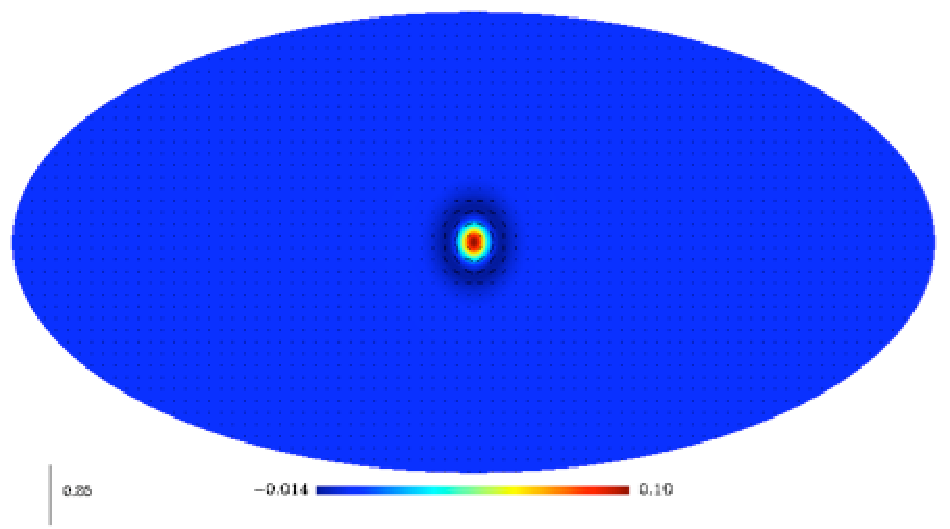
\includegraphics[width=7cm]{fig_e_iwt_back_scale2.pdf}
 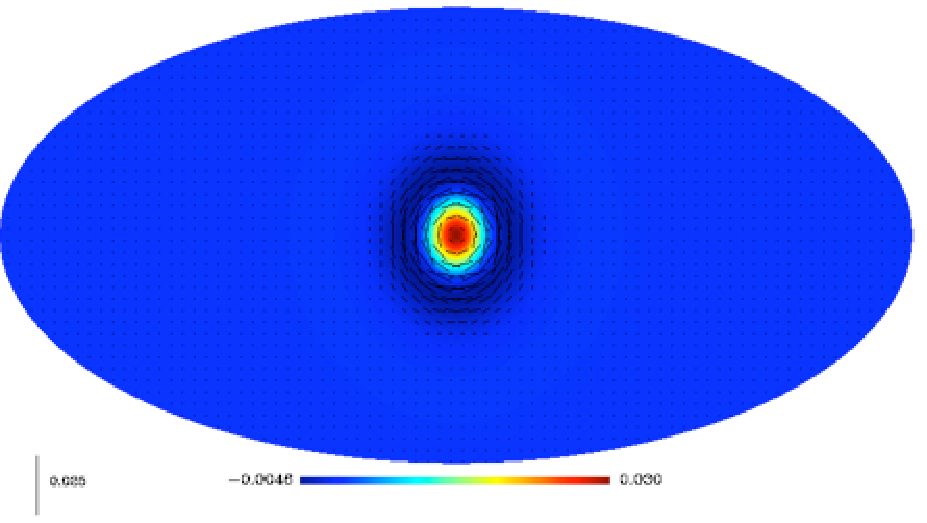
\includegraphics[width=7cm]{fig_b_iwt_back_scale2.pdf}
 }
  \hbox{
 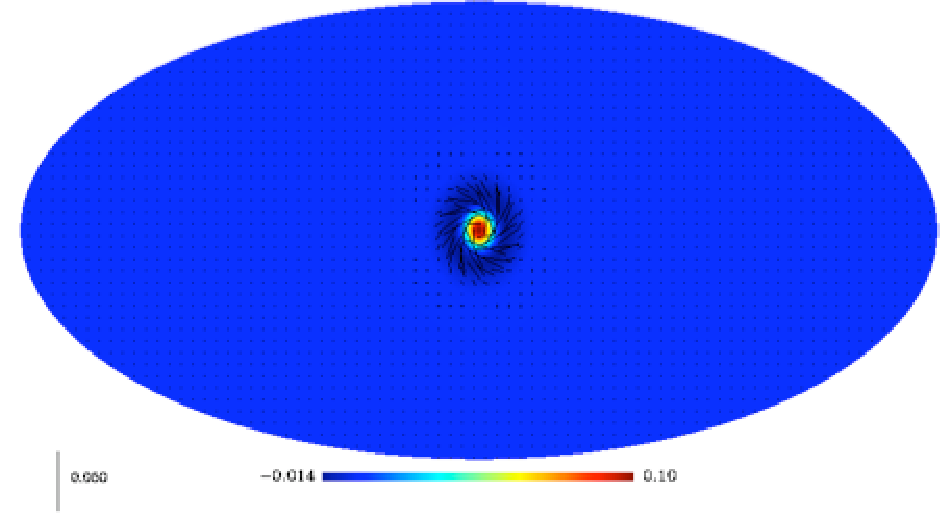
\includegraphics[width=7cm]{fig_e_iwt_back_scale3.pdf}
 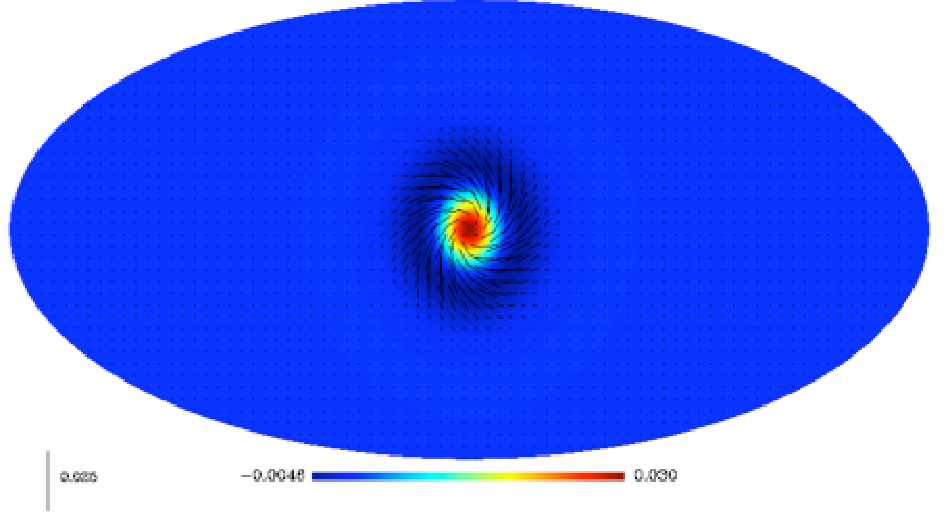
\includegraphics[width=7cm]{fig_b_iwt_back_scale3.pdf}
 }
 \hbox{
 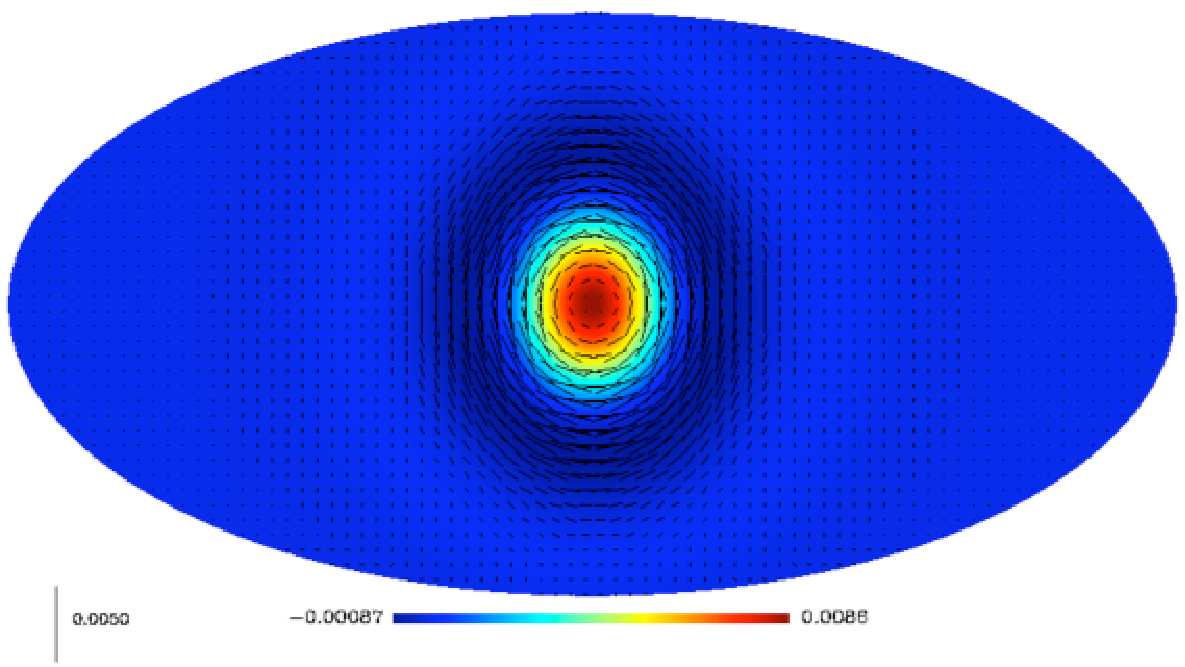
\includegraphics[width=7cm]{fig_e_iwt_back_scale4.pdf}
 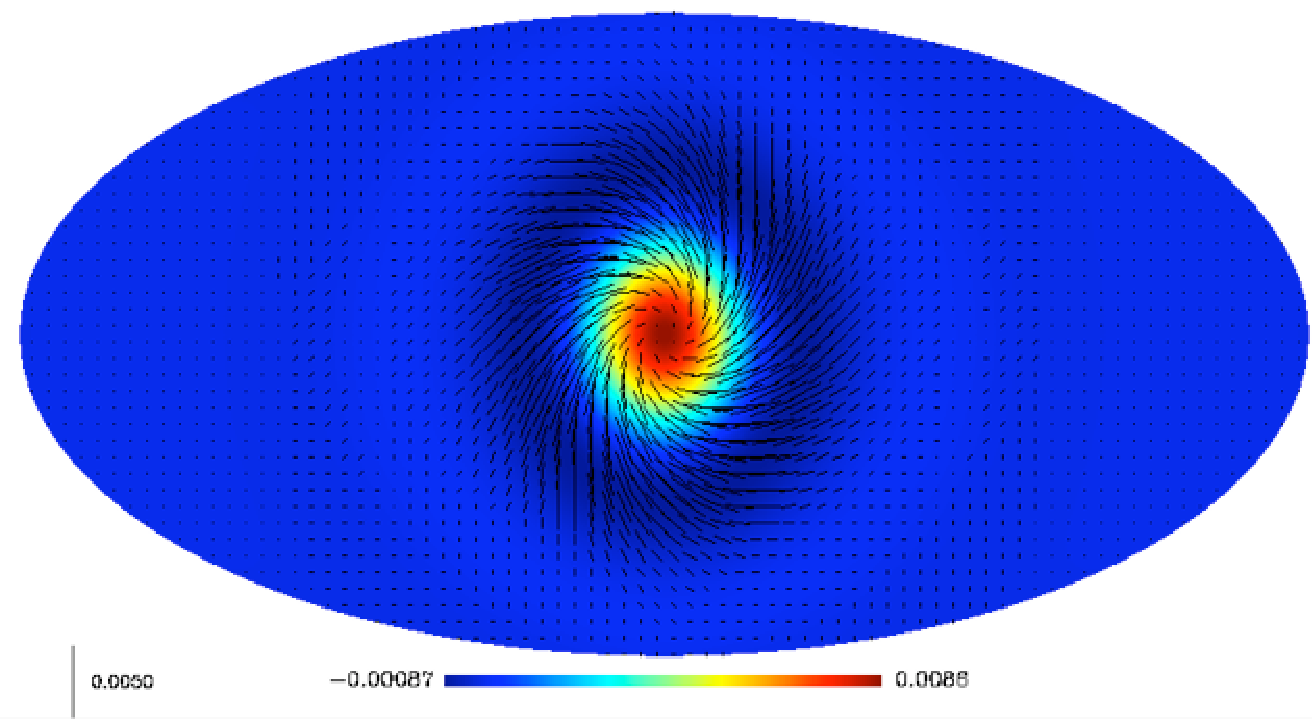
\includegraphics[width=7cm]{fig_b_iwt_back_scale4.pdf}
 }
 }
 }
\caption{E-isotropic wavelet transform backprojection (left) and B-isotropic wavelet backprojection (right).}
\label{fig_eb_iwt_back}
\end{figure*}
Obviously, the transform described above is invertible and the inverse transform is readily obtained by applying the inverse 
of each of the three steps in reverse order. If, as in the example decomposition above, we take the wavelet function to be 
the difference between two successive low pass approximations, the third step is inverted by simply summing the last low pass 
approximation with the maps of wavelet coefficients from all scales as in equation~\ref{IWT} : 
\begin{eqnarray}
T  & = & c_{J}^T + \sum_{j=1}^{J} w_j^T \quad \quad \nonumber \\
E & = & c_{J}^E + \sum_{j=1}^{J} w_j^E \quad \quad \nonumber \\
B & = &  c_{J}^B + \sum_{j=1}^{J} w_j^B
\end{eqnarray}
where $c_{J}^X$ stands for the low resolution approximation to component $X$ and $w_j^X$ is the map of wavelet coefficients of that component on scale $j$. Finally, noting that : 
\begin{eqnarray}
Q  & =  & -\frac{1}{2} \sum_{\ell, m}   a_{\ell m} ^E   ( {_{ 2} Y}_{\ell m} +  {_{ -2} Y}_{\ell m} ) +  i a_{\ell m} ^B ( {_{ 2} Y}_{\ell m} -  {_{ -2} Y}_{\ell m} )  \nonumber \\
     & =  & \sum_{\ell, m}   a_{\ell m} ^E   Z_{\ell m}^+ +  i a_{\ell m} ^B Z_{\ell m}^-   \\ \nonumber
U  & =   & -\frac{1}{2} \sum_{\ell, m}   a_{\ell m} ^B   ( {_{ 2} Y}_{\ell m} +  {_{ -2} Y}_{\ell m} ) -  i a_{\ell m} ^E ( {_{ 2} Y}_{\ell m} -  {_{ -2} Y}_{\ell m} )  \nonumber \\
      & =  & \sum_{\ell, m}   a_{\ell m} ^B Z_{\ell m}^+ -  i a_{\ell m} ^E Z_{\ell m}^-   
\end{eqnarray}
the initial representation of the polarized data in terms of $T$, $Q$ and $U$ maps is reconstructed from its wavelet coefficients using the following equations : 
% \begin{eqnarray}
%T= c_{J}^T + \sum_{j=1}^{J} w_j^T \\ \nonumber
%Q = \Big \{ \sum_{\ell, m}   <  c_{J}^E , Y_{\ell m}>  {_{ +} Z}_{\ell m} +  i <  c_{J}^B , Y_{\ell m}>  {_{ -} Z}_{\ell m} \Big \}        +   \sum_{j=1}^{J}  \Big \{ \sum_{\ell, m}  <  w_j^E , Y_{\ell m}>  {_{ +} Z}_{\ell m} +  i <  w_j^B , Y_{\ell m}>  {_{ -} Z}_{\ell m} \Big \}    \\ \nonumber 
%U = \Big \{ \sum_{\ell, m}   <  c_{J}^B , Y_{\ell m}>  {_{ +} Z}_{\ell m}  -  i <  c_{J}^E , Y_{\ell m}>  {_{ -} Z}_{\ell m} \Big \}        +   \sum_{j=1}^{J}  \Big \{ \sum_{\ell, m}  <  w_j^B , Y_{\ell m}>  {_{ +} Z}_{\ell m} -  i <  w_j^E , Y_{\ell m}>  {_{ -} Z}_{\ell m} \Big \}    
%\end{eqnarray}
%\begin{eqnarray}
%T =& c_{J}^T + \sum_{j=1}^{J} w_j^T \\ \nonumber
%Q =& c_{J}^E  \sum_{\ell, m} Y_{\ell m}^{\dagger} Z_{\ell m}^+ + i c_{J}^B  \sum_{\ell, m} Y_{\ell m} ^{\dagger} Z_{\ell m}^-  +   \sum_{j=1}^{J}  \Big \{  w_j^E  \sum_{\ell, m} Y_{\ell m}^{\dagger} Z_{\ell m}^+ +{i} w_j^B  \sum_{\ell, m} Y_{\ell m}^{\dagger}  Z_{\ell m}^- \Big \}    \\ \nonumber 
%U =& c_{J}^B  \sum_{\ell, m} Y_{\ell m}^{\dagger} Z_{\ell m}^+ -  i c_{J}^E  \sum_{\ell, m} Y_{\ell m} ^{\dagger} Z_{\ell m}^-  +   \sum_{j=1}^{J}  \Big \{  w_j^B  \sum_{\ell, m} Y_{\ell m}^{\dagger} Z_{\ell m}^+ - {i} w_j^E  \sum_{\ell, m} Y_{\ell m}^{\dagger}  Z_{\ell m}^- \Big \}   
%\end{eqnarray}
\begin{eqnarray}\label{eq:recons}
T =& c_{J}^T + \sum_{j=1}^{J} w_j^T \\ \nonumber
Q =& c_{J}^{E,+} + i c_{J}^{B,-} + \sum_{j=1}^{J} \Big \{ w_j^{E,+} + i w_j^{B,-} \Big \} \\ \nonumber 
U =& c_{J}^{B,+} - i c_{J}^{E,-} + \sum_{j=1}^{J} \Big \{ w_j^{B,+} - i w_j^{E,-} \Big \}
\end{eqnarray}
where
\begin{eqnarray}\label{eq:change}
c_{J}^{X,+} = c_{J}^X \sum_{\ell, m} Y_{\ell m}^{\dagger} Z_{\ell m}^+ \quad \textrm{and} \quad c_{J}^{X,-} = c_{J}^X \sum_{\ell, m} Y_{\ell m}^{\dagger} Z_{\ell m}^- 
\end{eqnarray}
with $W^\dagger$ denoting the transpose conjugate of $W$ so that $\tilde{W} W^\dagger$ is the scalar dot product of $\tilde{W}$ and $W$ 
while $W^\dagger \tilde{W}$ is an operator (or matrix) acting on its left hand side as a projection along $W$ and \emph{reconstruction} 
along $\tilde{W}$. In practice, the Healpix software package provides us with an implementation of the forward and inverse spin $0$ and 
spin $2$ spherical harmonics transforms which we need to implement the proposed inverse transform given by equations~\ref{eq:recons} 
and~\ref{eq:change}. Clearly, as mentioned earlier in section~\ref{sec:UWTS}, we could have chosen some other wavelet function than merely 
the difference between two consecutive scaling functions, and the transformation would still be nearly as simple to invert. Fig.\ref{fig_eb_iwt_back} 
shows, on the left, backprojections of E-wavelet coefficients, and, on the right, backprojections of B-wavelet coefficients on the right hand side at different scales.

%---------------------------------------------------------------------------------------------------------------------------------------
\subsection*{E-B  Curvelet}
%---------------------------------------------------------------------------------------------------------------------------------------
\begin{figure*}[htb]
\centerline{
\vbox{
 \hbox{
 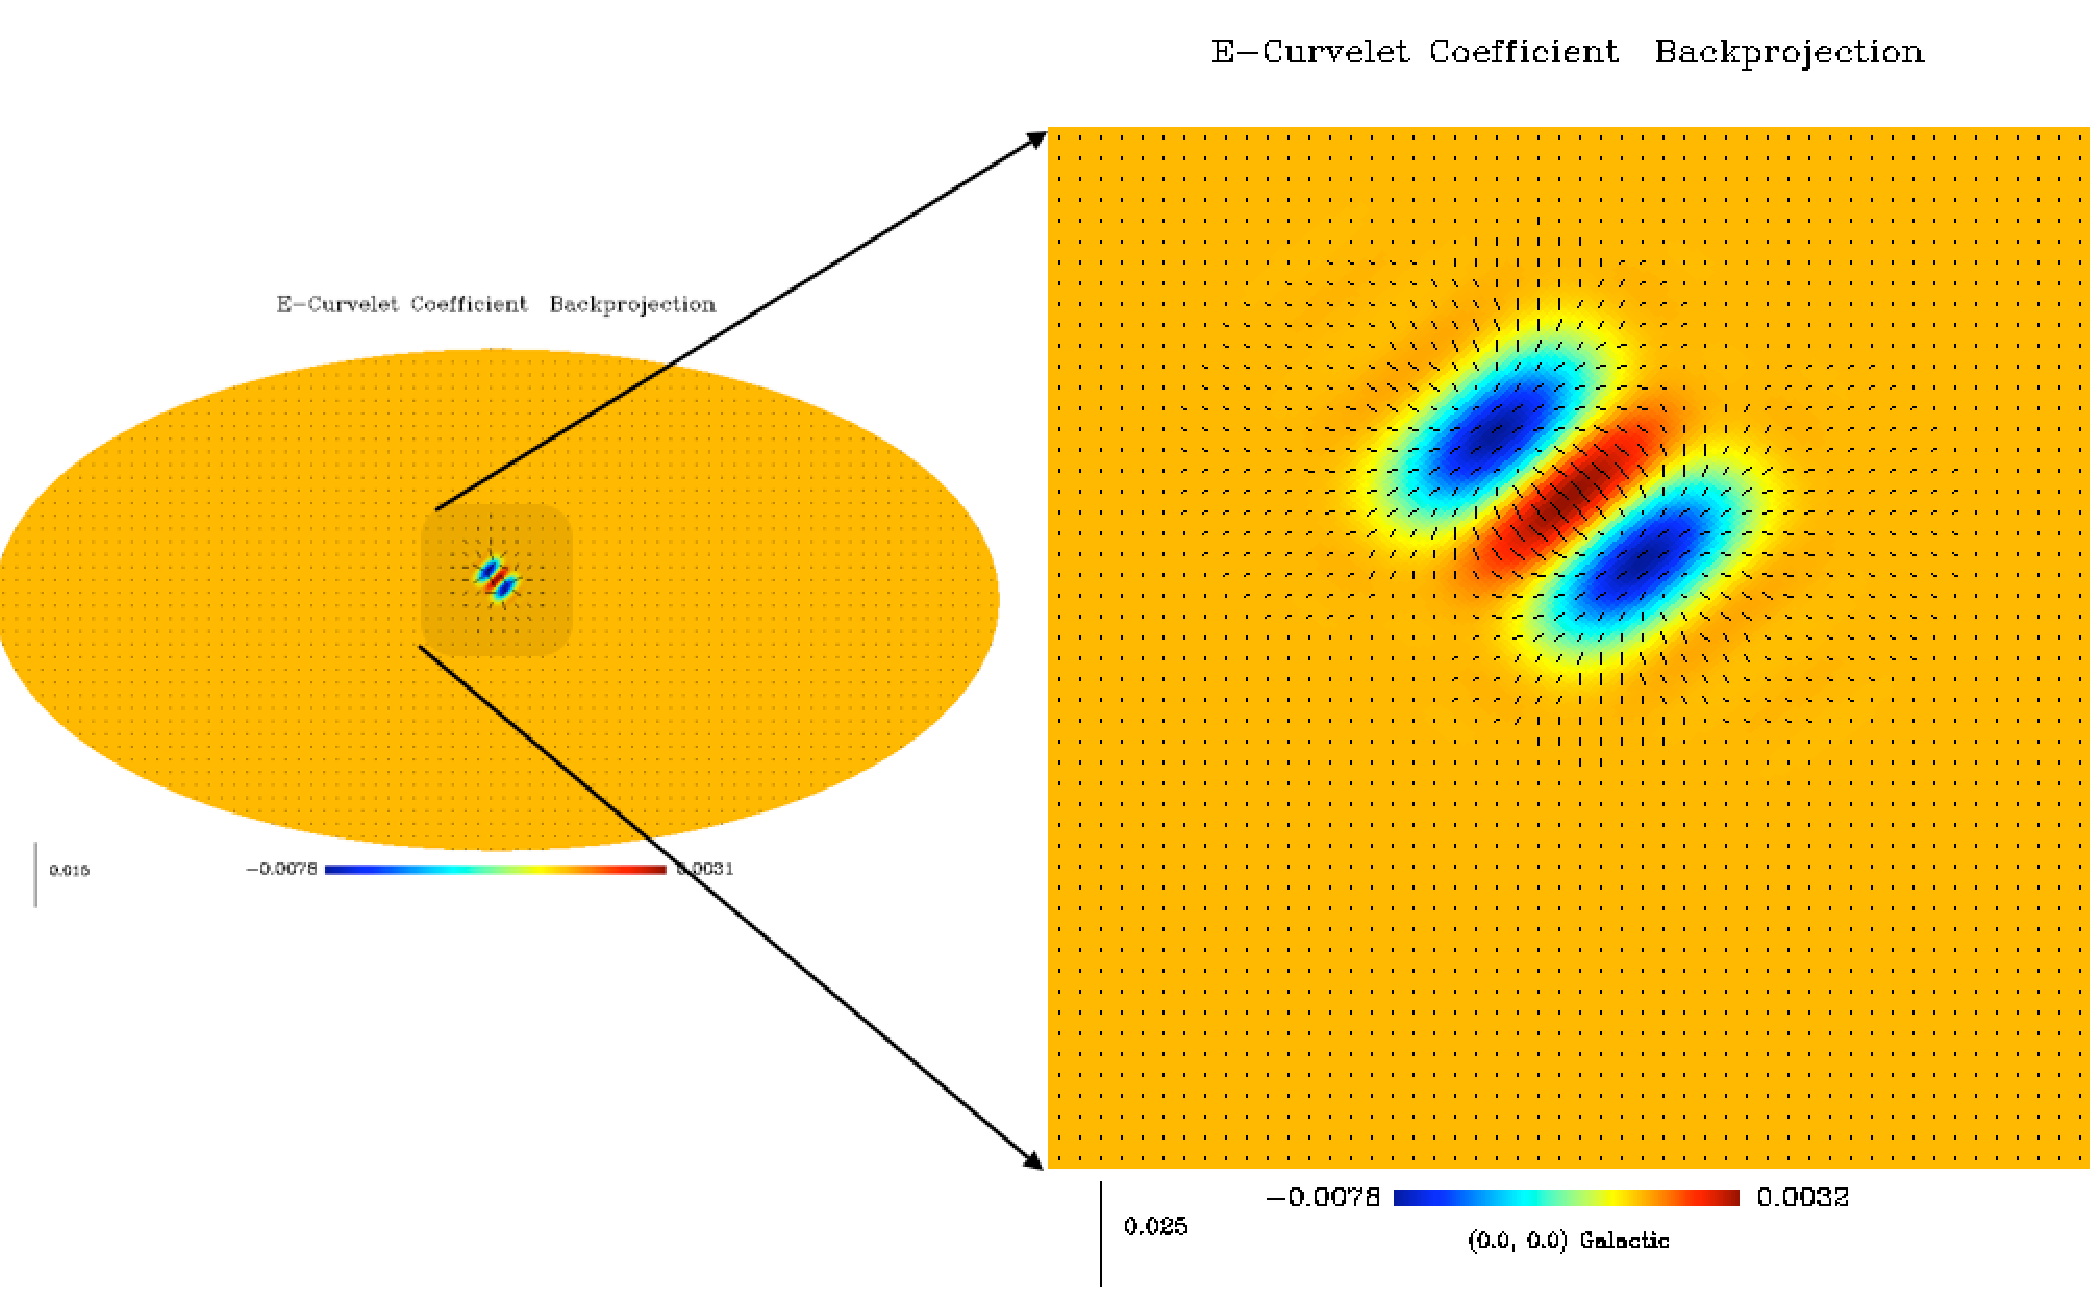
\includegraphics[width=12cm]{fig_ecur_back.pdf}
 }
  }
 }
\caption{E-curvelet coefficient backprojection.}
\label{fig_ecur_back}
\end{figure*}

\begin{figure*}[htb]
\centerline{
\vbox{
 \hbox{
 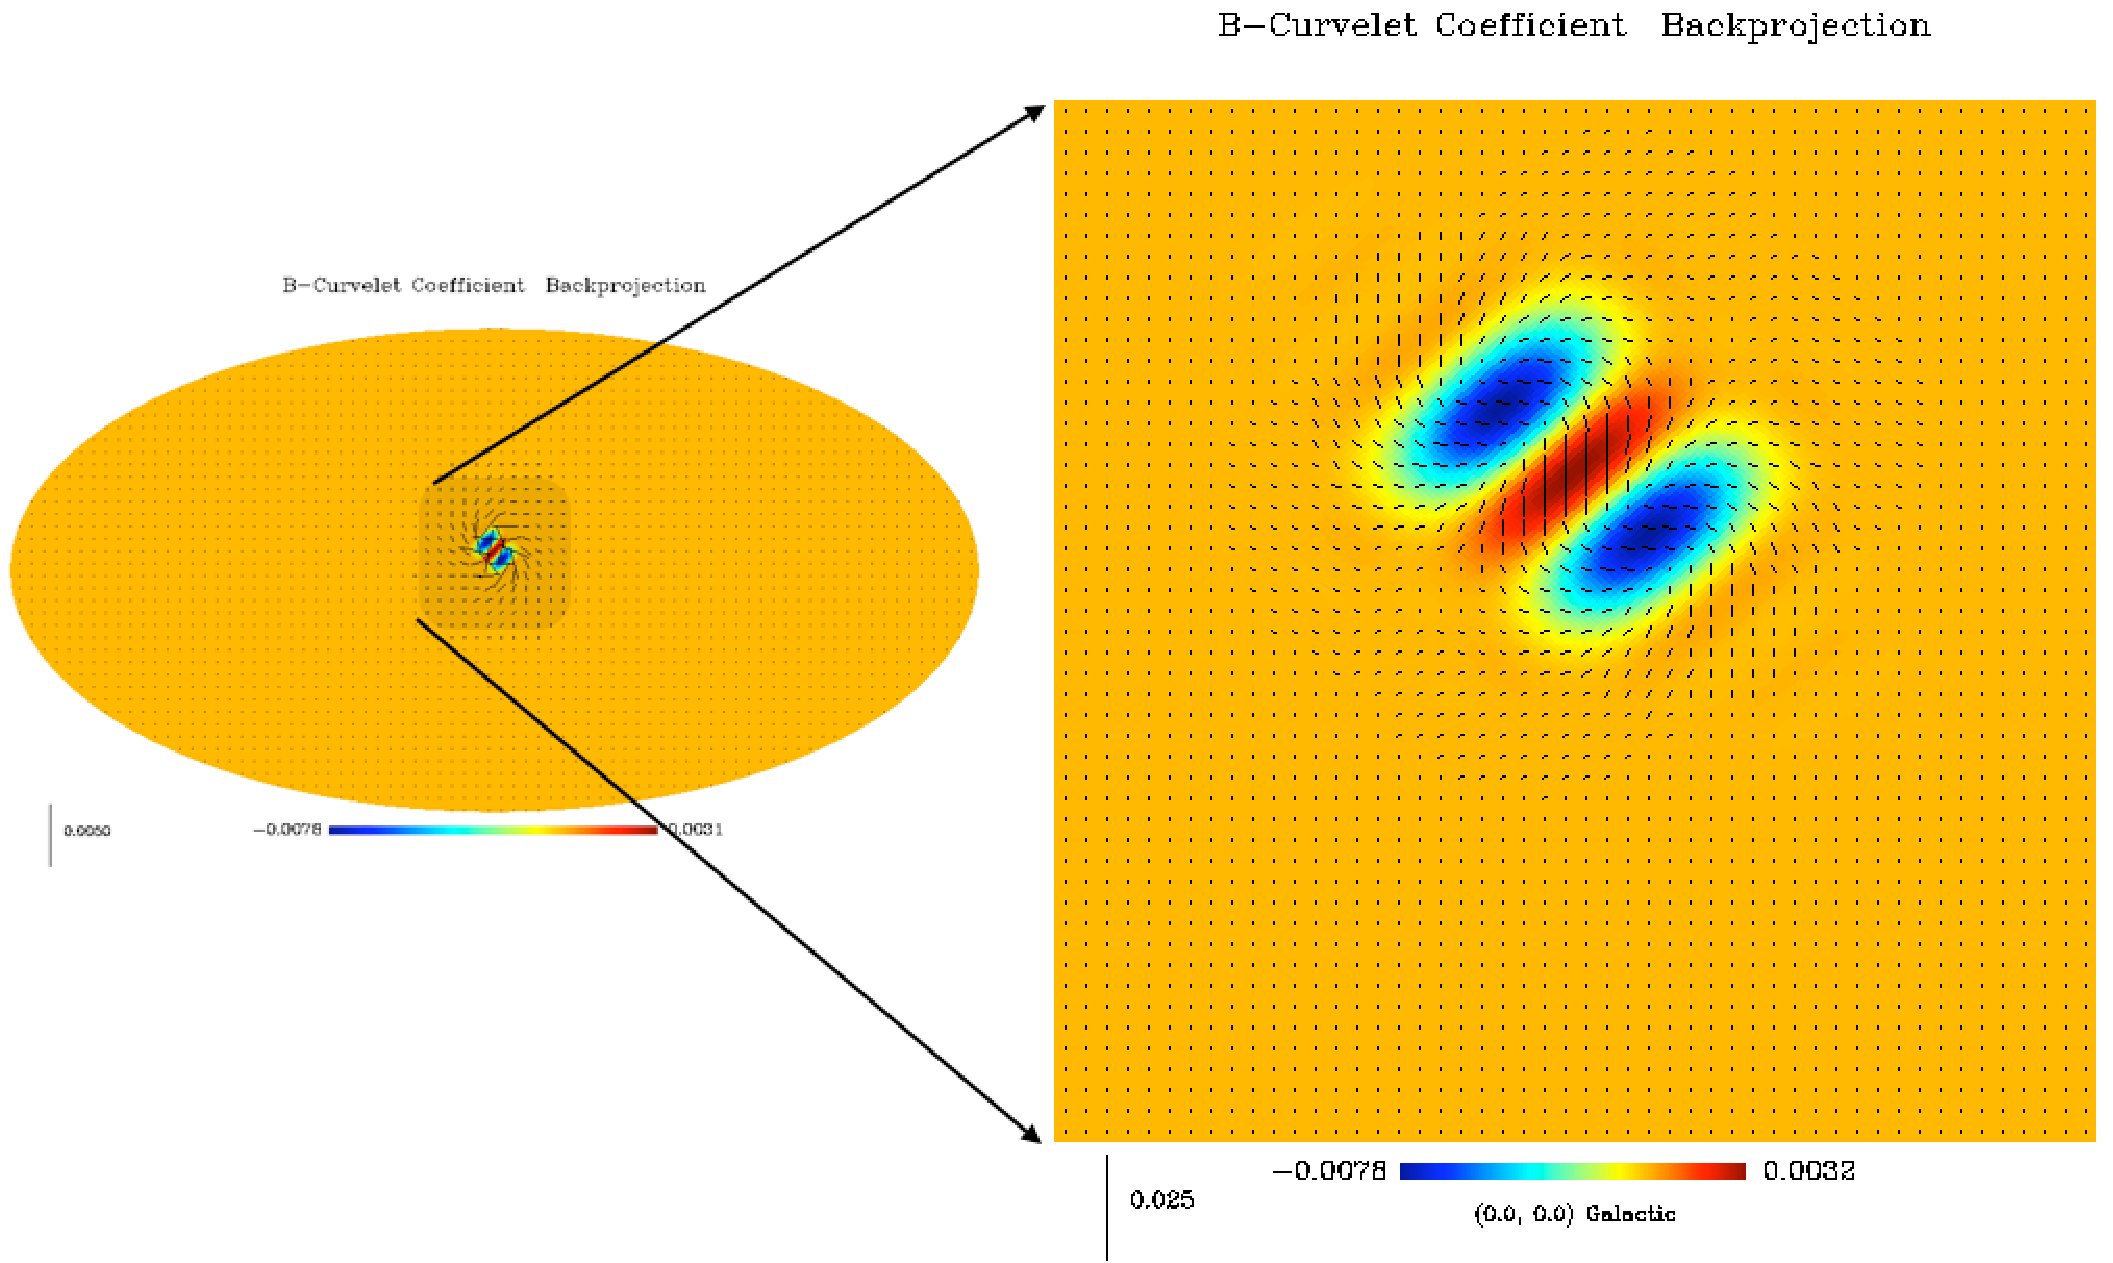
\includegraphics[width=12cm]{fig_bcur_back.pdf}
 }
 }
 }
\caption{B-curvelet coefficient backprojection.}
\label{fig_bcur_back}
\end{figure*}
Similarly to the EB-wavelet constructions, we can easily construct an EB-curvelet transform by first computing the E and B components using 
the spin $\pm 2$ spherical harmonics transform, and then applying a curvelet transform on the sphere separately on each of these two components.
Fig.~\ref{fig_ecur_back} shows the backprojection of an E-curvelet coefficient and Fig.~\ref{fig_bcur_back} shows the backprojectionof a B-curvelet coefficient.

%---------------------------------------------------------------------------------------------------------------------------------------
  

\chapter{IDL Routines}
\label{ch_mrsp_idl}
%\chapterhead{IDL Routines}
\markright{IDL Routines}


\section{Introduction}
A set of routines has been developed in IDL. Starting IDL using the script program {\em isap.pro} allows the user 
to get the interactive sparse data analysis  environment, and all routines described in the following can be called. 
An online help facility is also available by invoking the {\em isaph} program under IDL. See Chapter~\ref{ch_install} for more
details on the software installation.
  
\section{Functions for polarized spherical maps}
\index{polar}

\subsection{Reading a polarized spherical map from a file : mrsp\_read}
\index{IDL routines!mrsp\_read}
\index{polar!read polarized map}
Read a polarized spherical map in Healpix format.
{\bf
\begin{center}
     USAGE: map = mrsp\_read( file, noverb=noverb )
\end{center}}
where
\begin{itemize}
\item {\em file} : Input string, name of the file to be read. The pathname can be included in the string, by default 'file.fits' is equivalemt to './file.fits'
\item {\em noverb} : scalar, prevent the printing on the screen of the format (RING or NESTED) of the read map and the number of pixels.
\item {\em map} : Output 3D IDL array of Healpix map read. The map is setted to the NESTED format after reading.
\end{itemize}

\subsubsection*{Examples:} 
\begin{itemize}
\item map = mrsp\_read( 'my\_file\_healpix\_pola.fits', noverb=noverb ) \\
Read the map stored into the file 'my\_file\_healpix\_pola.fits' and load it into map.
\end{itemize}



\subsection{Writing a polarized spherical map into a file : mrsp\_write}
\index{IDL routines!mrsp\_write}
\index{polar!write polarized map}
Write a polarized spherical map in Healpix format.
{\bf
\begin{center}
     USAGE: mrsp\_write, file, map, ring=ring
\end{center}}
where
\begin{itemize}
\item {\em file} : Input string, name of the file to be writen. The pathname can be included in the string, by default 'file.fits' is equivalemt to './file.fits'
\item {\em map} : Input 3D IDL array of Healpix map to be writen. The map is assumed to be in the NESTED format.
\item {\em ring} : scalar, if set convert the Healpix map data to the RING format for the writing.
\end{itemize}



\subsection{Conversion of a polarized spherical map from TQU scheme to TEB scheme : mrsp\_tqu2teb}
\index{IDL routines!mrsp\_tqu2teb}
\index{polar!conversion tqu2teb}
Convert a polarized map in Healpix nested format from TQU scheme to TEB scheme.
{\bf
\begin{center}
     USAGE: mrsp\_tqu2teb, map\_tqu, map\_teb
\end{center}}
where
\begin{itemize}
\item {\em map\_tqu} : Input 3D IDL array of healpix polarized map in TQU scheme.
\item {\em map\_teb} : Output 3D IDL array of healpix polarized map in TEB scheme.
\end{itemize}



\subsection{Conversion of a polarized spherical map from TEB scheme to TQU scheme : mrsp\_teb2tqu}
\index{IDL routines!mrsp\_teb2tqu}
\index{polar!conversion tqu2teb}
Convert a polarized map in Healpix nested format from TEB scheme to TQU scheme.
{\bf
\begin{center}
     USAGE: mrsp\_teb2tqu, map\_teb, map\_tqu
\end{center}}
where
\begin{itemize}
\item {\em map\_teb} : Input 3D IDL array of healpix polarized map in TEB scheme.
\item {\em map\_tqu} : Output 3D IDL array of healpix polarized map in TQU scheme.
\end{itemize}



\subsection{Resizing a polarized spherical map: mrsp\_resize}
\index{IDL routines!mrsp\_resize}
\index{polar!polarized map resizing}
Resize a polarized map in Healpix nested format.
{\bf
\begin{center}
     USAGE: resize\_map = mrsp\_resize( map, nside=nside, ViaAlm=ViaAlm, teb=teb )
\end{center}}
where
\begin{itemize}
\item {\em map} : Input 3D IDL array of healpix polarized map in TQU scheme to be transformed.
\item {\em resize\_map} : Output 3D IDL array of healpix polarized map in TQU scheme. Healpix input map and output resized map are in nested format.
\item {\em nside} : int, the new nside parameter of the output healpix resized map.
\item {\em ViaAlm} : scalar, if set use alm transform for the resizing, otherwise, use interpolation. 
Ignored if nside keyword value is lower than imag nside.
\item {\em teb} : scalar, if set specifies that the input and output images are in TEB scheme.
\end{itemize}

\subsubsection*{Examples:} 
\begin{itemize}
\item map2 = mrsp\_resize( map, nside = 256, /ViaAlm ) \\
resize an Healpix map.
\end{itemize}





\section{General transform/reconstruction routines}

\subsection{Transformations of a polarized spherical map : mrsp\_trans}
\index{IDL routines!mrsp\_trans}
\index{polar!transforms of polarized image}
Compute a transform (E-B mode decomposition, wavelet with spline, Meyer or needelet filters, curvelet, \ldots) 
on a polarized map on the sphere in the Healpix representation (nested data representation) in TQU scheme.\\ \\
The transform can be:
\begin{enumerate}
\item A E/B decomposition using the spin\_2 transform.
\item An orthogonal wavelet on each T,Q,U component.
\item A pyramidal isotropic wavelet on each T,Q,U component.
\item An undecimated wavelet transform on each component.
\item A decimated modulus-Phase wavelet transform.
\item A undecimated modulus-Phase wavelet transform.
\item A curvelet transform.
\end{enumerate}
{\bf
\begin{center}
     USAGE: mrsp\_trans, Imag, Trans, NbrScale=NbrScale, lmax=lmax, MeyerWave=MeyerWave, ebdec=ebdec, Cur=Cur, uwt=uwt, owt=owt, mpdwt=mpdwt, mpuwt=mpuwt, PyrWT=PyrWT, 
     DifInSH=DifInSH, Overlap=Overlap, FirstBlockSize=FirstBlockSize
\end{center}}
where
\begin{itemize}
\item {\em Imag} : Input 3D IDL array of healpix polarized map in TQU scheme. Input image to be transformed.
\item {\em Trans} : Output IDL structure with the following fields:
\begin{itemize}
\item {\em NbrScale} : int, number of scales.
\item {\em nside} : int, Healpix nside parameter.
\item {\em lmax} : int, maximum l value in the Spherical Harmonic Space.
\item {\em npix} : long, number of pixels of the input image.
\item {\em MeyerWave} : int, 1 if the keyword MeyerWave used, otherwise 0.
\item {\em DifInSH} : int, 1 if the keyword DifInSH used, otherwise 0.
\item {\em pyrtrans} : int, 1 if a pyramidal decomposition has been applied, otherwise 0.
\item {\em ebdec} : int, 1 if an EB decomposiiton has been applied, otherwise 0.
\item {\em DEC1} : IDL structure, first component transformation (depends on the chosen transform).
\item {\em DEC2} : IDL structure, second component transformation (depends on the chosen transform).
\item {\em DEC3} : IDL structure, third component transformation (depends on the chosen transform).
\item {\em TransChoice} : string, code of the chosen transform.
\item {\em TabCodeTransform} : string array, array of transforms codes. TabCodeTransform = ['T\_EBDEC', 'T\_OWT', 'T\_PyrWT', 'T\_UWT', 'T\_MPDWT', 'T\_MPUWT', 'T\_CUR']
\item {\em TransName} : string, transform's name.
\item {\em TransTypeName} : string array, array of transforms names. 
TransTypeName = ['EBDEC','Bi-Orthogonal WT', 'Pyramidal WT', 'Undecimated WT', 'Module-Phase Decimated Transform', 'Module-Phase Undecimated Transform', 'Curvelet']
\end{itemize}
\item {\em NbrScale} : int, number of scales of the wavelet transforms.
\item {\em ebdec} : scalar, if set an E/B decomposition is applied before the chosen multiscale decomposition. 
If no transform is selected, it will be the default transformation.
\item {\em Cur} : scalar, if set perform a curvelet transform.
\item {\em uwt} : scalar, if set perform an undecimated isotropic wavelet transform.
\item {\em PyrWT} : scalar, if set perform a pyramidal isotropic wavelet transform.
\item {\em owt} : scalar, if set perform a bi-orthogonal wavelet transform on each face.
\item {\em mpdwt} : scalar, if set perform a decimated module-phase wavelet transform.
\item {\em mpuwt} : scalar, if set perform a undecimated module-phase wavelet transform.
\item {\em Overlap} : int, if equal to 1 if blocks are overlapping, only used with curvelet transform.
\item {\em FirstBlockSize} : int, block size in the ridgelet transform at the finest scale (default is 16), only used with curvelet transform.
\item {\em lmax} : int, maximum l value in the Spherical Harmonic Space (for isoptropic wavelet transform only).
\item {\em DifInSH} : Input keyword parameter. If set, the wavelet coefficients are computed as the difference between two resolutions in the spherical harmonics representation. 
Otherwise, the wavelet coefficients are computed as the difference between two resolutions in direct space. Only used with keyword uwt or PyrWT.
\item {\em MeyerWave} : If set, use Meyer wavelets and set the keyword DifInSH. Only used with keyword uwt or PyrWT.
\end{itemize}

\subsubsection*{Examples:} 
\begin{itemize}
\item mrsp\_trans, Imag, WT, NbrScale=5, /uwt \\
Compute the undecimated wavelet transform of the map Imag with five scales. The result is stored in WT.
\end{itemize}



\subsection{Reconstructions of a polarized spherical map : mrsp\_rec}
\index{IDL routines!mrsp\_rec}
\index{polar!inverse transform of polarized image}
Compute a inverse transform (wavelet, curvelet, \ldots) to get a polarized map on the sphere in the Healpix representation 
(nested data representation) in TQU scheme from its decomposition obtained by mrsp\_trans.\\ \\
The transform can be:
\begin{enumerate}
\item A E/B decomposition using the spin\_2 transform.
\item An orthogonal wavelet on each T,Q,U component.
\item A pyramidal isotropic wavelet on each T,Q,U component.
\item An undecimated wavelet transform on each component.
\item A decimated modulus-Phase wavelet transform.
\item A undecimated modulus-Phase wavelet transform.
\item A curvelet transform.
\end{enumerate}
{\bf
\begin{center}
     USAGE: mrsp\_rec, Trans, Rec
\end{center}}
where
\begin{itemize}
\item {\em Trans} : Input IDL structure, see mrsp\_trans for more details.
\item {\em Rec} : Output 3D IDL array of healpix polarized map in TQU scheme. Reconstructed image.
\end{itemize}

\subsubsection*{Examples:} 
\begin{itemize}
\item mrsp\_trans, Imag, WT, NbrScale=5, /uwt \\
Compute the undecimated wavelet transform of the map Imag with five scales. The result is stored in WT.
\item mrsp\_rec, WT, RecIma \\
Reconstruct the image.
\end{itemize}



\section{Spin-2 spherical harmonic transform}
 
\subsection{ALM transform of a polarized spherical map : mrsp\_almtrans}
\index{IDL routines!mrsp\_almtrans}
\index{polar!polar ALM transform}
Computes the spherical harmonic transform of a polarized TQU map using the Healpix representation (nested data).
{\bf
\begin{center}
     USAGE: mrsp\_almtrans, Imag, Trans, lmax=lmax, tab=tab, complex=complex, norm=norm, fast=fast
\end{center}}
where
\begin{itemize}
\item {\em Imag} : Input 3D IDL array of healpix polarized map in TQU scheme to be transformed.
\item {\em Trans} : Output IDL structure with the following fields:
\begin{itemize}
\item {\em ALM} : array of the ALM coefficients
\begin{center}
ALM = fltarray[*,2,3] list of the real part (ALM[*,0,*]) and imaginary part (ALM[*,1,*]) of the ALM. 
This is the default storage, ALM[*,*,0] is ALM T, ALM[*,*,1] is ALM E and ALM[*,*,2] is ALM B\\
ALM = cfarr[*,3] list of the ALM in complex values format if the keyword complex is set. 
ALM[*,0] is ALM T, ALM[*,1] is ALM E and ALM[*,2] is ALM B\\
ALM = fltarray[NbrMaxM, NbrMaxL, 2, 3] table of the real part (ALM[*,*,0,*]) and imaginary part (ALM[*,*,1,*]) 
of the ALM if the keyword tab is set. ALM[*,*,*,0] is ALM T, ALM[*,*,*,1] is ALM E and ALM[*,*,*,2] is ALM B\\
ALM = cfarr[NbrMaxM, NbrMaxL, 3] table of the ALM in complex values format if the keywords complex and tab 
are both setted. ALM[*,*,0] is ALM T, ALM[*,*,1] is ALM E and ALM[*,*,2] is ALM B\\
By default, NbrMaxM = NbrMaxL = lmax+1
\end{center}
\item {\em complex\_alm} : int, 0 (default value) if ALM array contains real and imaginary part separated. 
1 if ALM is a complex array.
\item {\em PixelType} : int, 0 for a Healpix input map (1 for GLESP but not used).
\item {\em tab} : int, 0 for default ALM representation as a list (i.e. 1D IDL array) and 1 for 2D 
representation as a table (i.e. l for the first dimension and m for the second).
\item {\em nside} : int, Healpix nside parameter.
\item {\em lmax} : int, maximum l value in the Spherical Harmonic Space.
\item {\em npix} : long, number of pixels of the input image.
\item {\em TabNbrM} : int array[NbrMaxL], max number of m value for a given l, only used if keyword tab is set otherwise, 0.
\item {\em index} : long array, indicies of the ALM coefficients, used only if keyword tab is not set.
\item {\em NormVal} : float, normalization value applied to the alm coefficients (only if keyword norm used).
\item {\em norm} : int, 0 if no normalization has been aplied, else 1.
\end{itemize}
\item {\em lmax} : int, Number of spherical harmonics computed in the decomposition. For a Healpix map, default is 
3*nside and should be between 2*nside and 4*nside.
\item {\em tab} : scalar, if set, ALM coefficients in Trans.alm are stored in a 2D array: Trans.alm[m,l] where m = 0..Trans.TabNbrM[l]-1  and l = 0..lmax-1
\item {\em complex} : scalar, if set Trans.alm will contain complex values instead of the real and imaginary parts.
\item {\em norm} : scalar, if set, a normalization is performed to the alm coefficients.
\end{itemize}

\subsubsection*{Example:} 
\begin{itemize}
\item mrsp\_almtrans, Imag, Output \\
Compute the spherical harmonics transform of a polarized image, the result is stored in Output.
\end{itemize}



\subsection{ALM inverse transform of a polarized spherical map : mrsp\_almrec}
\index{IDL routines!mrsp\_almrec}
\index{polar!polar ALM inverse transform}
Computes the inverse spherical harmonic transform of a polarized TQU map using using the Healpix representation (nested data).
{\bf
\begin{center}
     USAGE: mrsp\_almrec, Trans, imag, pixel\_window=pixel\_window
\end{center}}
where
\begin{itemize}
\item {\em Trans} : Input IDL structure of ALM coefficients, see mrsp\_almtrans above for details.
\item {\em Imag} : Output 3D IDL array of healpix polarized map in TQU scheme. Image reconstructed in Healpix nested representation.
\item {\em pixel\_window} : scalar, if set the image is convolved by the healpix pixel window (only for Healpix map).
\end{itemize}


\subsubsection*{Example:} 
\begin{itemize}
\item mrsp\_almtrans, PolaImag, Output \\
Compute the spherical harmonics transform of a polarized image, the result is stored in Output.
\item mrsp\_almrec, Output, PolaRec \\
Reconstruct the image.
\end{itemize}



\subsection{Power spectrum and cross spectrum exctraction from polarized ALM~: mrsp\_alm2spec}
\index{IDL routines!mrsp\_alm2spec}
\index{polar!spectrum exctraction from polarized ALM}
Computes the power spectrums and cross spectrums of a polarized map from the polarized ALM coefficients.
{\bf
\begin{center}
     USAGE: spec = mrsp\_alm2spec( ALM, StdPS=StdPS )
\end{center}}
where
\begin{itemize}
\item {\em ALM} : Input IDL structure of ALM polarized coefficients, see mrsp\_almtrans above for details.
\item {\em spec} : Output 2D IDL float array[ALM.lmax+1,6], the TT, EE, BB, TE, TB, EB spectrums. P[k,i] = Mean( SPECTRUM[*,l,i] ) \quad i=0...5.
\item {\em StdPS} : Output 2D IDL float array[ALM.lmax+1,6]: estimated standard deviation of the spectrums coefficients.
\end{itemize}

\subsubsection*{Example:} 
\begin{itemize}
\item mrsp\_almtrans, Imag, Output \\
Compute the spherical harmonics transform of a polarized image, the result is stored in Output.
\item spec = mrsp\_alm2spec( Output, StdPS=StdPS ) \\
Compute the spectrums of the image and it's associated standard deviation.
\end{itemize}


\subsection{Power spectrum and cross spectrum exctraction from a polarized image : mrsp\_spec}
\index{IDL routines!mrsp\_spec}
\index{polar!spectrum exctraction from a polarized image}
Computes the power spectrums and cross spectrums of a polarized map, using the HEALPix representation (nested data representation by default). 
By default a normalisation is applied on the ALM coefficents.
{\bf
\begin{center}
     USAGE: spec = mrsp\_spec( Imag, nonorm=nonorm, teb=teb, NormVal=NormVal, StdPS=StdPS, lmax=lmax )
\end{center}}
where
\begin{itemize}
\item {\em Imag} : Input 3D IDL array of healpix polarized map in TQU scheme. Input image whose power spectrum will be extracted.
\item {\em spec} : Output 2D IDL float array[ALM.lmax+1,6], the TT, EE, BB, TE, TB, EB spectrums. P[k,i] = Mean( SPECTRUM[*,l,i] ) \quad i=0...5.
\item {\em Lmax} : int, number of spherical harmonics computed in the decomposition and size of the computed spectrum (Lmax+1). Default is 3*nside and should be between 2*nside and 4*nside.
\item {\em nonorm} : scalar, if set no normalisation is applied on the ALM computed.
\item {\em StdPS} : Output 2D IDL float array[ALM.lmax+1,6]: estimated standard deviation of the spectrums coefficients.
\item {\em NormVal} : float, normalization value applied to the alm coefficients.
\item {\em teb} : scalar, if set specifies that the input map is in TEB scheme.
\end{itemize}

\subsubsection*{Example:} 
\begin{itemize}
\item P = mrsp\_spec( Imag ) \\
Compute the spectrum of the polarized image.
\end{itemize}



\section{Polarized Wavelets}
\subsection{Undecimated Isotropic Wavelet Transform of a polarized spherical map : mrsp\_wttrans}
\index{IDL routines!mrsp\_wttrans}
\index{polar!undecimated wavelet transform of polarized image}
Computes the undecimated isotropic wavelet transform of polarized maps on the sphere in TQU scheme, 
using the Healpix representation (nested data representation). The wavelet function is zonal and its 
spherical harmonics coefficients $a_{l,0}$ follow a cubic box-spline profile. If the keyword DifInSH is 
set, the wavelet coefficients are derived in the Spherical Harmonic Space, otherwise (default) they 
are derived in the direct space.
{\bf
\begin{center}
     USAGE: mrsp\_wttrans, Imag, Trans, NbrScale=NbrScale, lmax=lmax, DifInSH=DifInSH, MeyerWave=MeyerWave
\end{center}}
where
\begin{itemize}
\item {\em Imag} : Input 3D IDL array of healpix polarized map in TQU scheme. Input image to be transformed.
\item {\em Trans} : Output IDL structure with the following fields:
\begin{itemize}
\item {\em NbrScale} : int, number of scales.
\item {\em nside} : int, Healpix nside parameter.
\item {\em lmax} : int, maximum l value in the Spherical Harmonic Space.
\item {\em npix} : long, number of pixels of the input image.
\item {\em MeyerWave} : int, 1 if the keyword MeyerWave used, otherwise 0
\item {\em DifInSH} : int, 1 if the keyword DifInSH used, otherwise 0
\item {\em Coef} : fltarr[npix,NbrScale,3] wavelet transform of the data. Coef[*,*,0] = wavelet transform on T, Coef[*,*,1] = wavelet transform on E, Coef[*,*,2] = wavelet transform on B
\begin{center}
Coef[*,0,*] = wavelet coefficients of the finest scale (highest frequencies).\\
Coef[*,NbrScale-1,*] = coarsest scale (lowest frequencies). 
\end{center}
\end{itemize}
\item {\em NbrScale} : int, optional input parameter specifying the number of scales (default is 4).
\item {\em Lmax} : int, optional input parameter specifying the maximum multipole number $l$ in the spherical harmonics decomposition 
(default is $3\times \textrm{nside}$, should be between $2\times \textrm{nside}$ and $4\times \textrm{nside}$).
\item {\em DifInSH} : Input keyword parameter. If set, the wavelet coefficients are computed as the difference between two resolutions in the spherical harmonics representation. 
Otherwise, the wavelet coefficients are computed as the difference between two resolutions in direct space.
\item {\em MeyerWave} : If set, use Meyer wavelets and set the keyword DifInSH.
\end{itemize}

\subsubsection*{Example:} 
\begin{itemize}
\item mrsp\_wttrans, Imag, Output, NbrScale=5 \\
Compute the isotropic wavelet transform of the map Imag with five scales. The result is stored in Output.
\end{itemize}



\subsection{Undecimated Isotropic Wavelet Reconstruction of a polarized spherical map : mrsp\_wtrec}
\index{IDL routines!mrsp\_wtrec}
\index{polar!undecimated wavelet reconstruction of polarized image}
Reconstructs a polarized maps on the sphere in TQU scheme using the Healpix representation (nested data representation) 
from its wavelet coefficients obtained with the undecimated isotropic wavelet transform on the sphere, described right above.
{\bf
\begin{center}
     USAGE: mrsp\_wtrec, Trans, Rec, filter=filter
\end{center}}
where
\begin{itemize}
\item {\em Trans}: Input IDL structures with the following fields:  
\begin{itemize}
\item {\em NbrScale} : int, number of scales.
\item {\em nside} : int, Healpix nside parameter.
\item {\em lmax} : int, maximum l value in the Spherical Harmonic Space.
\item {\em npix} : long, number of pixels of the input image.
\item {\em MeyerWave} : int, 1 if the keyword MeyerWave used, otherwise 0
\item {\em DifInSH} : int, 1 if the keyword DifInSH used, otherwise 0
\item {\em Coef} : fltarr[npix,NbrScale,3] wavelet transform of the data. Coef[*,*,0] = wavelet transform on T, Coef[*,*,1] = wavelet transform on E, Coef[*,*,2] = wavelet transform on B
\begin{center}
Coef[*,0,*] = wavelet coefficients of the finest scale (highest frequencies).\\
Coef[*,NbrScale-1,*] = coarsest scale (lowest frequencies). 
\end{center}
\end{itemize}
\item {\em Rec} : Output 3D IDL array of healpix polarized map in TQU scheme. Reconstructed image from the wavelet coefficients. 
\item {\em filter} : Input keyword parameter. Use filters for the reconstructions. If this keyword is not set, the reconstructed image is obtained 
by a simple addition of all wavelet scales. Automaticaly applied if keyword MeyerWave or DifInSH were set at the wavelet decomposition.
\end{itemize}

\subsubsection*{Examples:} 
\begin{itemize}
\item mrsp\_wttrans, Imag, Output, NbrScale=5 \\
Compute the isotropic wavelet transform of the map Imag with five scales. The result is stored in Output.
\item mrsp\_wtrec, Output, map \\
Reconstruct the map. 
\end{itemize}





\subsection{Extract a scale from a polar decomposition : mrsp\_wtget}
\index{IDL routines!mrsp\_wtget}
\index{polar!polar wavelet extraction}
Return a band of a transform for Healpix polarized map (wavelet, curvelet\ldots) obtained by the command mrsp\_trans.
{\bf
\begin{center}
     USAGE:  Scale = mrsp\_wtget( Trans, Component, ScaleNumber, BandNumber=BandNumber, NormVal=NormVal )
\end{center}}
where
\begin{itemize}
\item {\em Trans} : Input IDL structure, see mrsp\_trans for more details.
\item {\em ScaleNumber} : int, scale number of the band to be extracted. The scale number must be between 0 and Trans.NbrScale-1.
\item {\em Component} : int, choice of the component, 0 is for T, 1 for E and 2 for B.
\item {\em NormVal} : float, optional normalization value of the band (for isotropic wavelet transform).
\item {\em BandNumber} : int, ridgelet band number (for curvelet transform).
\item {\em Scale} : return value IDL array of the band extracted. See more details on the 1D versions of the functions. 
No band is extracted from Modulus-Phases transforms (return 0). For a E/B decomposition, it will be either the T map, the E map or the B map.
\end{itemize}



\subsection{Put a scale into a polar decomposition : mrsp\_wtput}
\index{IDL routines!mrsp\_wtput}
\index{polar!polar wavelet insertion}
Put a band into a transform for Healpix polarized map (wavelet, curvelet\ldots) obtained by the command mrsp\_trans.
{\bf
\begin{center}
     USAGE:   mrsp\_wtput, Trans, Scale, Component, ScaleNumber, BandNumber=BandNumber
\end{center}}
where
\begin{itemize}
\item {\em Trans} : Input IDL structure, see mrsp\_trans for more details.
\item {\em Scale} : Input IDL array of the band inserted. See more details on the 1D versions of the functions. 
No band is inserted into Modulus-Phases transforms. For a E/B decomposition, it will be either the T map, the E map or the B map.
\item {\em ScaleNumber} : int, scale number of the band to be extracted. The scale number must be between 0 and Trans.NbrScale-1.
\item {\em Component} : int, choice of the component, 0 is for T, 1 for E and 2 for B.
\item {\em BandNumber} : int, ridgelet band number (for curvelet transform).
\end{itemize}



\section{Denoising}
\subsection{Wavelet filtering of a polarized spherical map : mrsp\_wtfilter}
\index{IDL routines!mrsp\_wtfilter}
\index{polar!polar wavelet filtering}
Wavelet denoising of a polarized image on the sphere using Healpix representation in TQU scheme (nested pixel representation). 
By default Gaussian noise is considered. If the keyword SigmaNoise is not set, then the noise standard deviation is automatically 
estimated. If the keyword MAD is set, then a correlated Gaussian noise is considered and the noise level at each scale is derived 
from the Median Absolution Deviation (MAD) method. If the keyword KillLastScale is set, the coarsest resolution is set to zero. 
The thresholded wavelet coefficients can be obtained using the keyword Trans. If the input keyword niter is set, then an iterative 
algorithm is applied and if the pos keyword is also set, then a positivity constraint is added.
{\bf
\begin{center}
     USAGE:  mrsp\_wtfilter, Imag, Filter, NbrScale=NbrScale, NSigma=NSigma, SigmaNoise=SigmaNoise, KillLastScale=KillLastScale, 
     pos=pos, mad=mad, Trans=Trans, niter=niter, FirstScale=FirstScale, Use\_FdrAll=Use\_FdrAll, soft=soft, fdr=fdr, lmax=lmax, 
     FilterLast=FilterLast, mask=mask 
\end{center}}
where
\begin{itemize}
\item {\em Imag} : Input 3D IDL array of healpix polarized map in TQU scheme. Input image to be filtered.
\item {\em Filter} : Output 3D IDL array of healpix polarized map in TQU scheme containing the filtered map.
\item {\em NbrScale} : int, number of scales (default is 4).
\item {\em NSigma} : float, level of thresholding (default is 3).
\item {\em SigmaNoise} : float, noise standard deviation. Default is automatically estimated.
\item {\em mad} : scalar, if set the noise level is derived at each scale using the MAD of the wavelet coefficient.
\item {\em KillLastScale} : scalar, if set the last scale is set to zero.
\item {\em niter} : int, number of iterations used in the reconstruction.
\item {\em pos} : scalar, if set the solution is assumed to be positive.
\item {\em FirstScale} : int, consider only scales larger than FirstScale. Default is 1 (i.e. all scales are used).
\item {\em Soft} : scalar, if set use soft thresholding instead of hard thresholding.
\item {\em fdr} : float between 0 (default) and 1 (max, if greater or equal to 1, set to 0.05), used to estimate a threshold level 
instead of a NSigma threshold, threshold is applied from scale j=FirstScale to the last.
\item {\em Use\_FdrAll} : same as fdr but applied to all scales.
\item {\em FilterLast} : scalar, if set the last scale is filtered.
\item {\em mask} : IDL array of healpix map, input mask applied.
\item {\em lmax} : int, maximum l value in the Spherical Harmonic Space.
\item {\em Trans} : IDL structure: Thresholded wavelet decomposition of the input image.
\end{itemize}


\subsubsection*{Example:} 
\begin{itemize}
\item mrsp\_wtfilter, Imag, Filter, NbrScale=5, Nsigma=5 \\
Wavelet filtering with five scales and a 5 sigma threshold.
\end{itemize}


\subsection{Thresholding in polarized wavelet or curvelet space  : mrsp\_threshold}
\index{IDL routines!mrsp\_threshold}
\index{polar!polar curvelet filtering}

Threshold the decomposition coefficients of a polarized healpix map. This routine works with several decompositions (see mrsp\_trans).
{\bf
\begin{center}
     USAGE:  mrsp\_threshold, Trans, NSigma=Nsigma, Mad=Mad, KillLastScale=KillLastScale
\end{center}}
where
where
\begin{itemize}
\item {\em Trans} : IDL structures obtained from the {\em mrsp\_trans} routine.
\item {\em Nsigma}: Level of thresholding (default is 3)
\item {\em KillLastScale}: if set, the last scale is set to zero
\end{itemize}

\subsubsection*{Examples:} 
 Compute the undecimated wavelet transform of a vector field I with five scales (needlet filters).  The result is stored in WT, then wavelet coefficients are threshold at 2 sigma, and the filtered polarized map is reconstructed.
\begin{itemize}
\item  mrsp\_trans, I, WT, NbrScale=5, /UWT, /NeedletWave
\item  mrsp\_threshold, WT, NSigma=2
\item  mrsp\_rec, WT, RecPola
\end{itemize}
Compute the curvelet transform of a vector field I with five scales.  The result is stored in C, then curvelet coefficients are threshold at 5 sigma, and the filtered polarized map 
is reconstructed.
\begin{itemize}
\item  mrsp\_trans, I, C, NbrScale=5, /Cur
\item  mrsp\_threshold, C, NSigma=5
\item  mrsp\_rec, C, RecPola
\end{itemize}
  

\part{\projmc: \defprojmc }

\chapter{Introduction}
\label{ch_msvst_intro}

Several techniques have been proposed in the literature to estimate Poisson intensity in 2D. A major class of methods adopt a multiscale bayesian framework specifically tailored for Poisson data~\citep{Nowak2000}, independently initiated by \citet{wave:timmermann99} and \citet{Kolaczyk1999}. \citet{Lefkimmiatis} proposed an improved bayesian framework for analyzing Poisson processes, based on a multiscale representation of the Poisson process in which the ratios of the underlying Poisson intensities in adjacent scales are modeled as mixtures of conjugate parametric distributions. Another approach includes preprocessing the count data by a variance stabilizing transform (VST) such as the Anscombe \citep{rest:anscombe48} and the Fisz \citep{rest:nason04} transforms, applied respectively 
in the spatial~\citep{rest:donoho93_2} or in the wavelet domain~\citep{Fryzlewicz2004}. The transform reforms the data so that the noise approximately becomes Gaussian with a constant variance. Standard techniques for independant identically distributed Gaussian noise are then used for denoising. \citet{starck:zhang07} proposed a powerful method called Multi-Scale Variance Stabilizing Tranform (MS-VST). It consists in combining a VST with a multiscale transform (wavelets, ridgelets or curvelets), yielding asymptotically normally distributed coefficients with known variances. The choice of the multi-scale method depends on the morphology of the data. Wavelets represent more efficiently regular structures and isotropic singularities, whereas ridgelets are designed to represent global lines in an image, and curvelets represent efficiently curvilinear contours. Significant coefficients are then detected with binary hypothesis testing, and the final estimate is reconstructed with an iterative scheme. In \citet{Starck09:fermi3d}, it was shown that sources can be detected in 3D FERMI LAT data (2D+time or 2D+energy) using a specific 3D extension of the MS-VST.
 \citet{Schmitt} proposed a method for Poisson intensity estimation on spherical data called Multi-Scale Variance Stabilizing Transform on the Sphere (MS-VSTS). This MS-VSTS (Multi-Scale Variance Stabilizing Transform on the Sphere) package offers a Poisson denoising method on the sphere, designed for Fermi photon counts maps.
This method is based on the MS-VST~\citep{starck:zhang07} and on multi-scale transforms on the sphere \citep{starck2006,inpainting:abrial06,starck:abrial08}.
 Chapter~\ref{ch_msvsts} introduces the MS-VSTS. 
 Chapter~\ref{ch_denoising} applies the MS-VSTS to spherical data restoration. Chapter~\ref{ch_inpainting} applies the MS-VSTS to inpainting. Chapter~\ref{ch_background} applies the MS-VSTS to background extraction. An accurate description of the IDL routines that makeup this package is given in Chapter~\ref{ch_idlproc}. An extension to multichannel denoising and deconvolution is given in Chapter~\ref{ch_multichannel} Conclusions are drawn in Chapter~\ref{ch_conclusion}. All experiments were performed on HEALPix maps with $nside=128$~\citep{pixel:healpix}, which corresponds to a good pixelisation choice for  data such as the GLAST/FERMI resolution. The performance of the method is not dependent on the nside parameter. For a given data set, if nside is small, it just means that we don't want to investigate the finest scales. If nside is large, the number of counts per pixel will be very small, and we may not have enough statistics to get any information at the finest resolution levels. But it will not have any bad effect on the solution. Indeed,  the finest scales
will be smoothed, since our algorithm will not detect any significant wavelet coefficients in the finest scales. Hence, starting with a fine pixelisation (i.e. large nside), our method will provide a kind of automatic binning, by thresholding wavelets coefficients at scales and at spatial positions where the number of counts is not sufficient.




% \newpage
  
\chapter{Multi-Scale Variance Stabilizing Transform on the Sphere (MS-VSTS)}
\label{ch_msvsts}

% \markright{Multi-Scale Variance Stabilizing Transform on the Sphere (MS-VSTS)}

\section{Principle of VST}

\subsection{VST of a Poisson process}

Given Poisson data $\mathbf{Y} := (Y_i)_i$, each sample $Y_i \sim \mathcal{P} (\lambda_i)$ has a variance $\text{Var}[Y_i] = \lambda_i$. Thus, the variance of $\mathbf{Y}$ is signal-dependant. The aim of a VST $\mathbf{ T}$ is to stabilize the data such that each coefficient of $\mathbf{ T}(\mathbf{Y})$ has an (asymptotically) constant variance, say $1$, irrespective of the value of $\lambda_i$. In addition, for the VST used in this study, $T(\mathbf{Y})$ is asymptotically normally distributed. Thus, the VST-transformed data are asymptotically stationary and gaussian.

The Anscombe transform \citep{rest:anscombe48} is a widely used VST which has a simple square-root form
\begin{equation}
\label{eq14}
\mathbf{ T}(Y):=2\sqrt{Y+3/8}.
\end{equation}
We can show that $\mathbf{ T}(Y)$ is asymptotically normal as the intensity increases.
\begin{equation}
\label{eq15}
\mathbf{ T}(Y)-2\sqrt{\lambda} \autorightarrow{$\mathcal{D}$}{$\lambda \rightarrow + \infty$} \mathcal{N}(0,1)
\end{equation}
It can be shown that the Anscombe VST requires a high underlying intensity to well stabilize the data (typically for $\lambda \geqslant 10$) \citep{starck:zhang07}.

\subsection{VST of a filtered Poisson process}

Let $Z_j := \sum_i h[i] Y_{j-i}$ be the filtered process obtained by convolving $(Y_i)_i$ with a discrete filter $h$. We will use $Z$ to denote any of the $Z_j$'s. Let us define $\tau_k := \sum_i (h[i])^k$ for $k=1,2,\cdots$. In addition, we adopt a local homogeneity assumption stating that $\lambda_{j-i} = \lambda$ for all $i$ within the support of $h$.

We define the square-root transform $T$ as follows:
\begin{equation}
\label{eq16}
T(Z):=b\cdot \mathrm{sign}(Z+c) |Z+c|^{1/2},
\end{equation}
where $b$ is a normalizing factor.  \\
\emph{\textbf{(Square root as VST)}} If $\tau_1 \neq 0$, $\|h\|_2,\|h\|_3<\infty$, then we have : \\
\begin{equation} \label{eq17}
\begin{split}
\mathrm{sign}(Z+c)\sqrt{|Z+c|}-\mathrm{sign}(\tau_1)\sqrt{|\tau_1|\lambda} \\
 \autorightarrow{$\mathcal{D}$}{$\lambda \rightarrow + \infty$} \mathcal{N}\Big(0,\frac{\tau_2}{4|\tau_1|}\Big).
\end{split}
\end{equation}
This  proves that $T$ is a VST for a filtered Poisson process (with a nonzero-mean filter) in that $T(Y)$ is asymptotically normally distributed with a stabilized variance as $\lambda$ becomes large (see \citet{starck:zhang07} for a proof).


\section{MS-VSTS}


The MS-VSTS~\citep{Schmitt} consists in combining the square-root VST with a multi-scale transform on the sphere.

\subsection{MS-VSTS + IUWT}

This section describes the MS-VSTS + IUWT, which is a combination of a square-root VST with the IUWT. The recursive scheme is:
\begin{equation}
\label{eq27}
\begin{split}
&\text{IUWT}\left\{\begin{array}{ccc}a_j  & = &  h_{j-1} \ast a_{j-1}  \\d_j  & = & a_{j-1}  - a_j  \end{array}\right. \\
 \Longrightarrow & \begin{split}\text{MS-VSTS} \\  \text{+ IUWT} \end{split}\left\{\begin{array}{ccc}a_j  & = &  h_{j-1} \ast a_{j-1} \\d_j  & = & T_{j-1}(a_{j-1}) - T_j(a_j) \end{array}\right. .
\end{split}
\end{equation}

In (\ref{eq27}), the filtering on $a_{j-1}$ can be rewritten as a filtering on $a_0 := \mathbf{Y}$, i.e., $a_j = h^{(j)} \ast a_0$, where $h^{(j)} = h_{j-1} \ast \cdots \ast h_{1} \ast h_0$ for $j \geqslant 1$ and $h^{(0)} = \delta$, where $\delta$ is the Dirac pulse ($\delta = 1$ on a single pixel and $0$ everywhere else). $T_j$ is the VST operator at scale $j$:
\begin{equation}
\label{eq28}
T_j(a_j) = b^{(j)} \mathrm{sign}(a_j+c^{(j)})\sqrt{|a_j + c^{(j)}|} .
\end{equation}
Let us define $\tau_k^{(j)}:=\sum_i (h^{(j)}[i])^k$. In~\citet{starck:zhang07}, it has ben shown that, to have an optimal convergence rate for the VST, the constant $c^{(j)}$ associated to $h^{(j)}$ should be set to:
\begin{equation}
\label{eq29}
c^{(j)}:=\frac{7\tau_2^{(j)}}{8\tau_1^{(j)}} - \frac{\tau_3^{(j)}}{2\tau_2^{(j)}} .
\end{equation}
The MS-VSTS+IUWT procedure is directly invertible as we have:
\begin{equation}
\label{eq30}
a_0 (\theta,\varphi) = T_0^{-1} \Bigg[ T_J(a_J) + \sum_{j=1}^J d_j \Bigg] (\theta,\varphi).
\end{equation}
Setting $b^{(j)}:=\text{sgn}(\tau_1^{(j)})/\sqrt{|\tau_1^{(j)}|}$, if $\lambda$ is constant within the support of the filter.
$h^{(j)}$, then we have \citep{starck:zhang07}:
\begin{equation}
\label{eq31}
\begin{split}
d_j(\theta,\varphi) \autorightarrow{$\mathcal{D}$}{$\lambda \rightarrow + \infty$} 
\mathcal{N} \Bigg( 0 , \frac{\tau_2^{(j-1)}}{4\tau_1^{(j-1)^2}} +\\ \frac{\tau_2^{(j)}}{4\tau_1^{(j)^2}} - \frac{\langle h^{(j-1)},h^{(j)} \rangle}{2\tau_1^{(j-1)}\tau_1^{(j)}} \Bigg) ,
\end{split}
\end{equation}
where $\langle . , . \rangle$ denotes inner product.

It means that the detail coefficients issued from locally homogeneous parts of the signal follow asymptotically a central normal distribution with an intensity-independant variance which relies solely on the filter $h$ and the current scale for a given filter $h$. Consequently, the stabilized variances and the constants $b^{(j)}$,$c^{(j)}$,$\tau_k^{(j)}$ can all be pre-computed.
Let us define $\sigma_{(j)}^2$ the stabilized variance at scale $j$ for a locally homogeneous part of the signal:
\begin{equation}
\label{eq32}
\sigma_{(j)}^2 = \frac{\tau_2^{(j-1)}}{4\tau_1^{(j-1)^2}} + \frac{\tau_2^{(j)}}{4\tau_1^{(j)^2}} - \frac{\langle h^{(j-1)},h^{(j)} \rangle}{2\tau_1^{(j-1)}\tau_1^{(j)}} .
\end{equation}

To compute the $\sigma_{(j)}$, $b^{(j)}$,$c^{(j)}$,$\tau_k^{(j)}$, we only have to know the filters $h^{(j)}$. We compute these filters thanks to the formula $a_j = h^{(j)} \ast a_0$, by applying the IUWT to a Dirac pulse $a_0 = \delta$. Then, the $h^{(j)}$ are the scaling coefficients of the IUWT. The $\sigma_{(j)}$ have been precomputed for a 6-scaled IUWT (Table~\ref{sigmaj}). 

\begin{table*}[!h]
  \centering
    \caption{Precomputed values of the variances $\sigma_j$ of the wavelet coefficients.
  }
  \begin{tabular}{|c|c|}
\hline
Wavelet scale $j$ & Value of $\sigma_j$ \\
\hline
  1 & 0.484704 \\
  2 & 0.0552595 \\
  3 & 0.0236458 \\
  4 & 0.0114056 \\
  5 & 0.00567026 \\
\hline
\end{tabular}

  \label{sigmaj}
\end{table*}

We have simulated Poisson images of different constant intensities $\lambda$, computed the IUWT with MS-VSTS on each image and observed the variation of the normalized value of $\sigma_{(j)}$ ($\mathbf{ (\sigma_{(j)})_{\text{simulated}}} / (\sigma_{(j)})_{\text{theoretical}}$) as a function of $\lambda$ for each scale $j$ (Fig. \ref{sigma}). We see that the wavelet coefficients are stabilized when $\lambda \gtrsim 0.1$ except for the first wavelet scale, which is mostly constituted of noise. On Fig. \ref{ansc}, we compare the result of MS-VSTS with Anscombe + wavelet shrinkage, on sources of varying intensities. We see that MS-VSTS works well on sources of very low intensities, whereas Anscombe doesn't work when the intensity is too low.

\begin{figure}[htb]
\centering{
\hbox{
%\psfig{figure=sigma1.ps,widtht=2.9in}
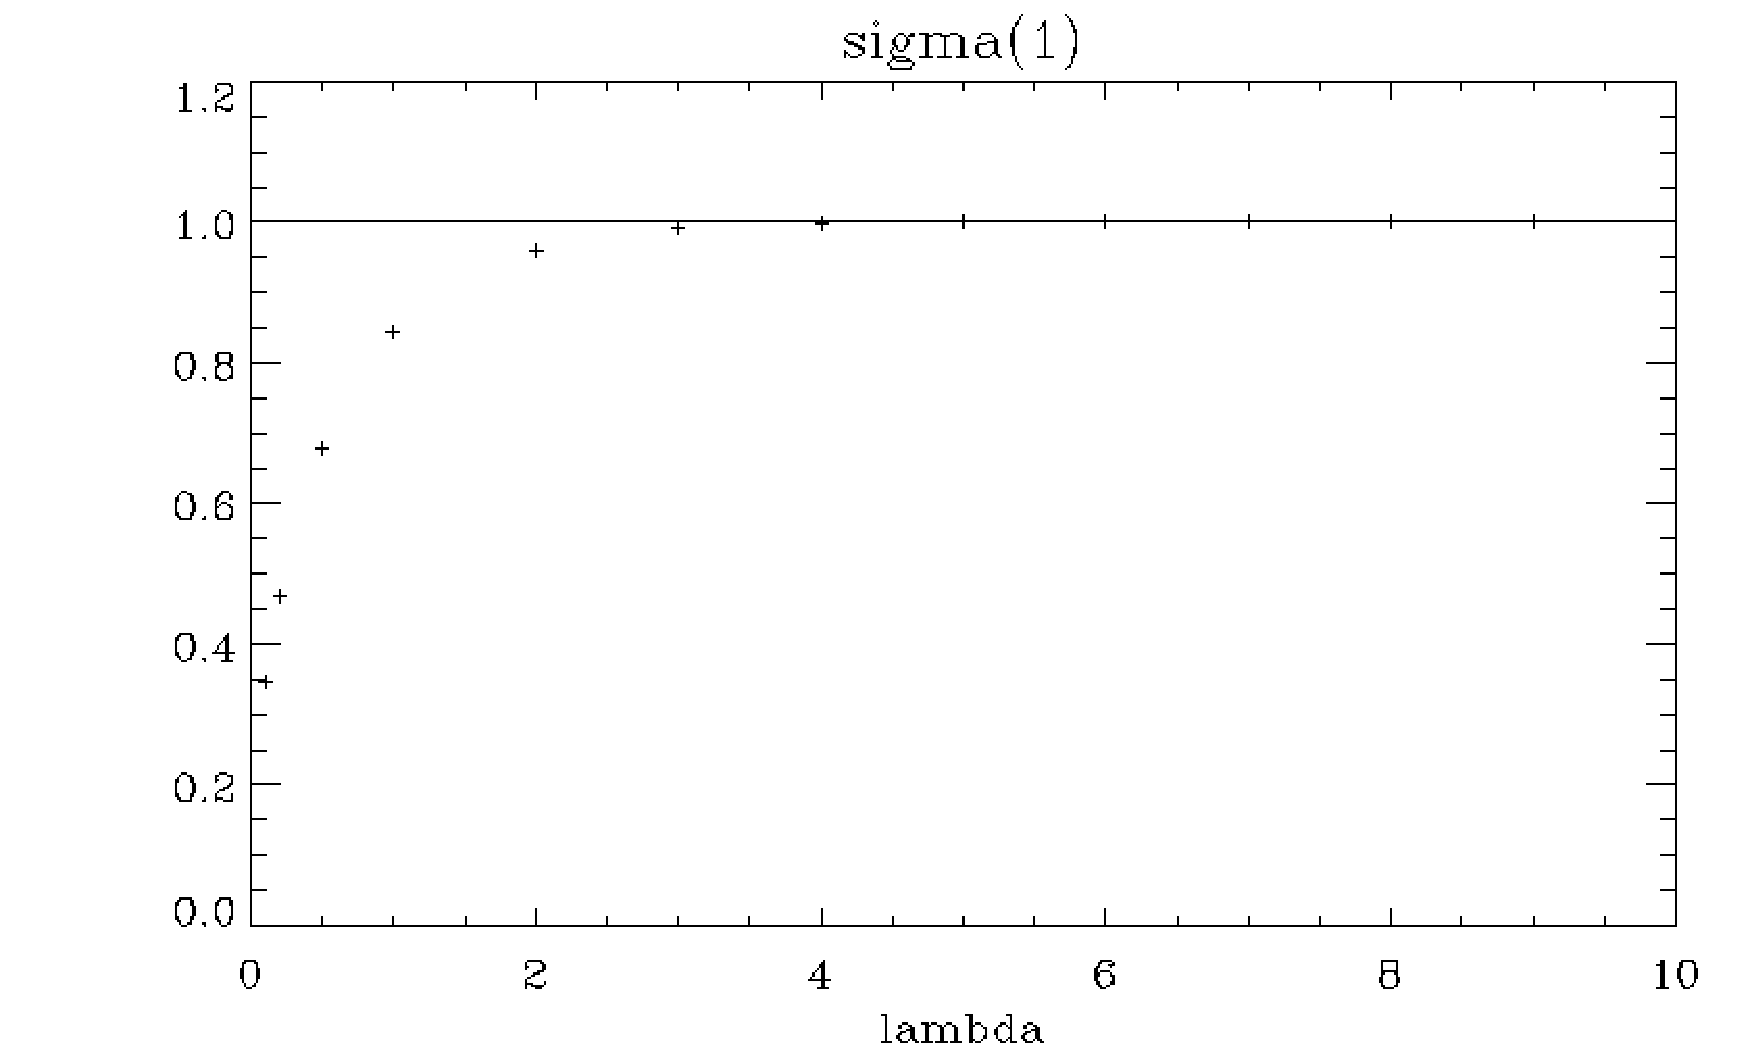
\includegraphics[width=2.5in, height=3in]{13822fg1.pdf}
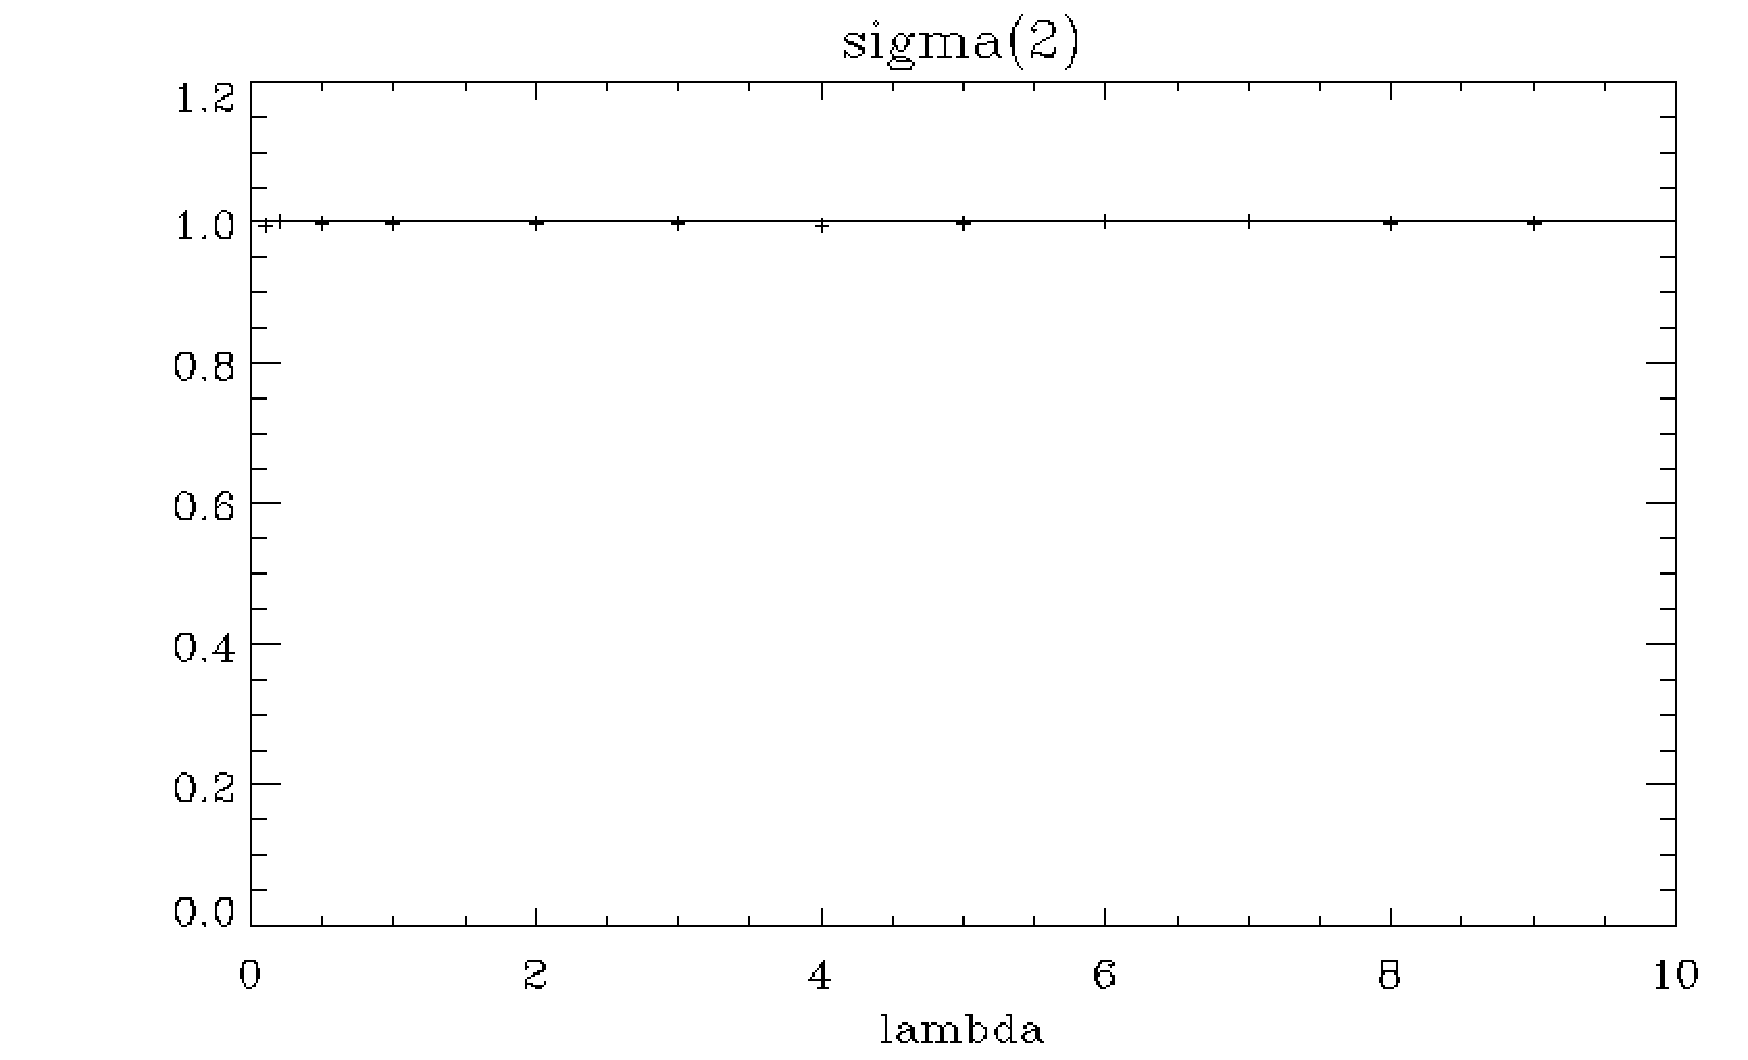
\includegraphics[width=2.5in, height=3in]{13822fg2.pdf}
}
\hbox{
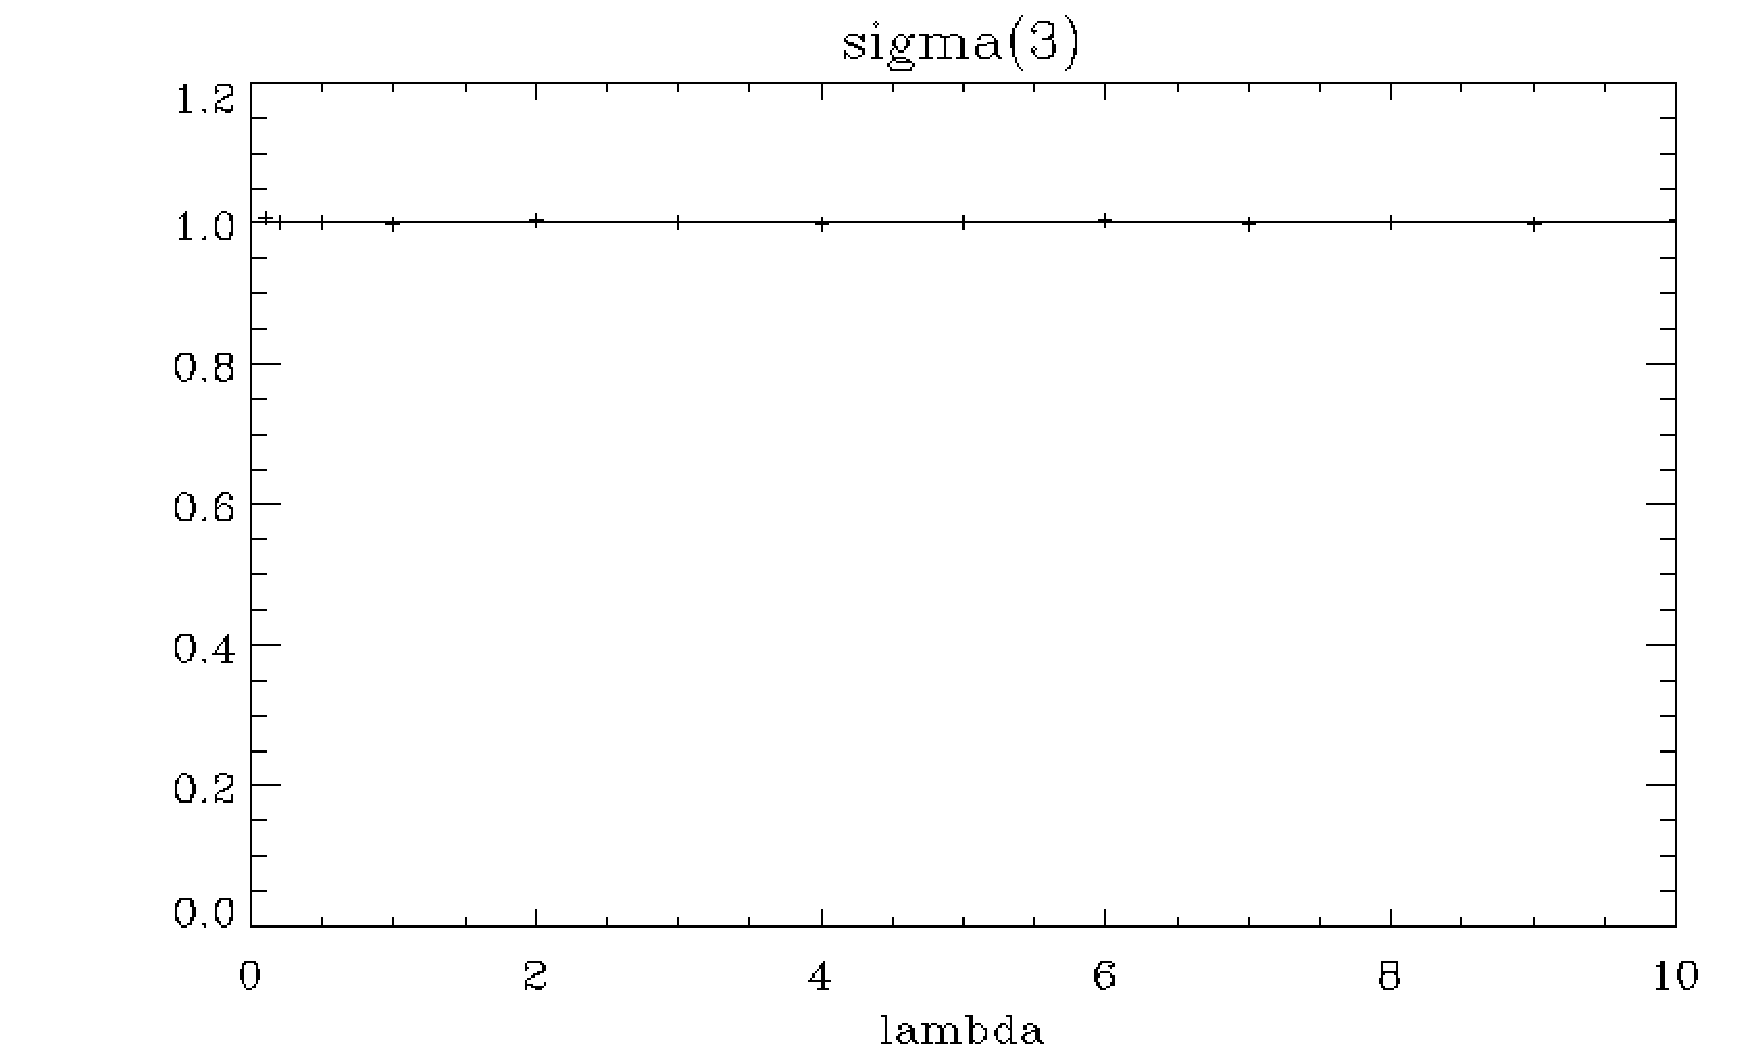
\includegraphics[width=2.5in, height=3in]{13822fg3.pdf}
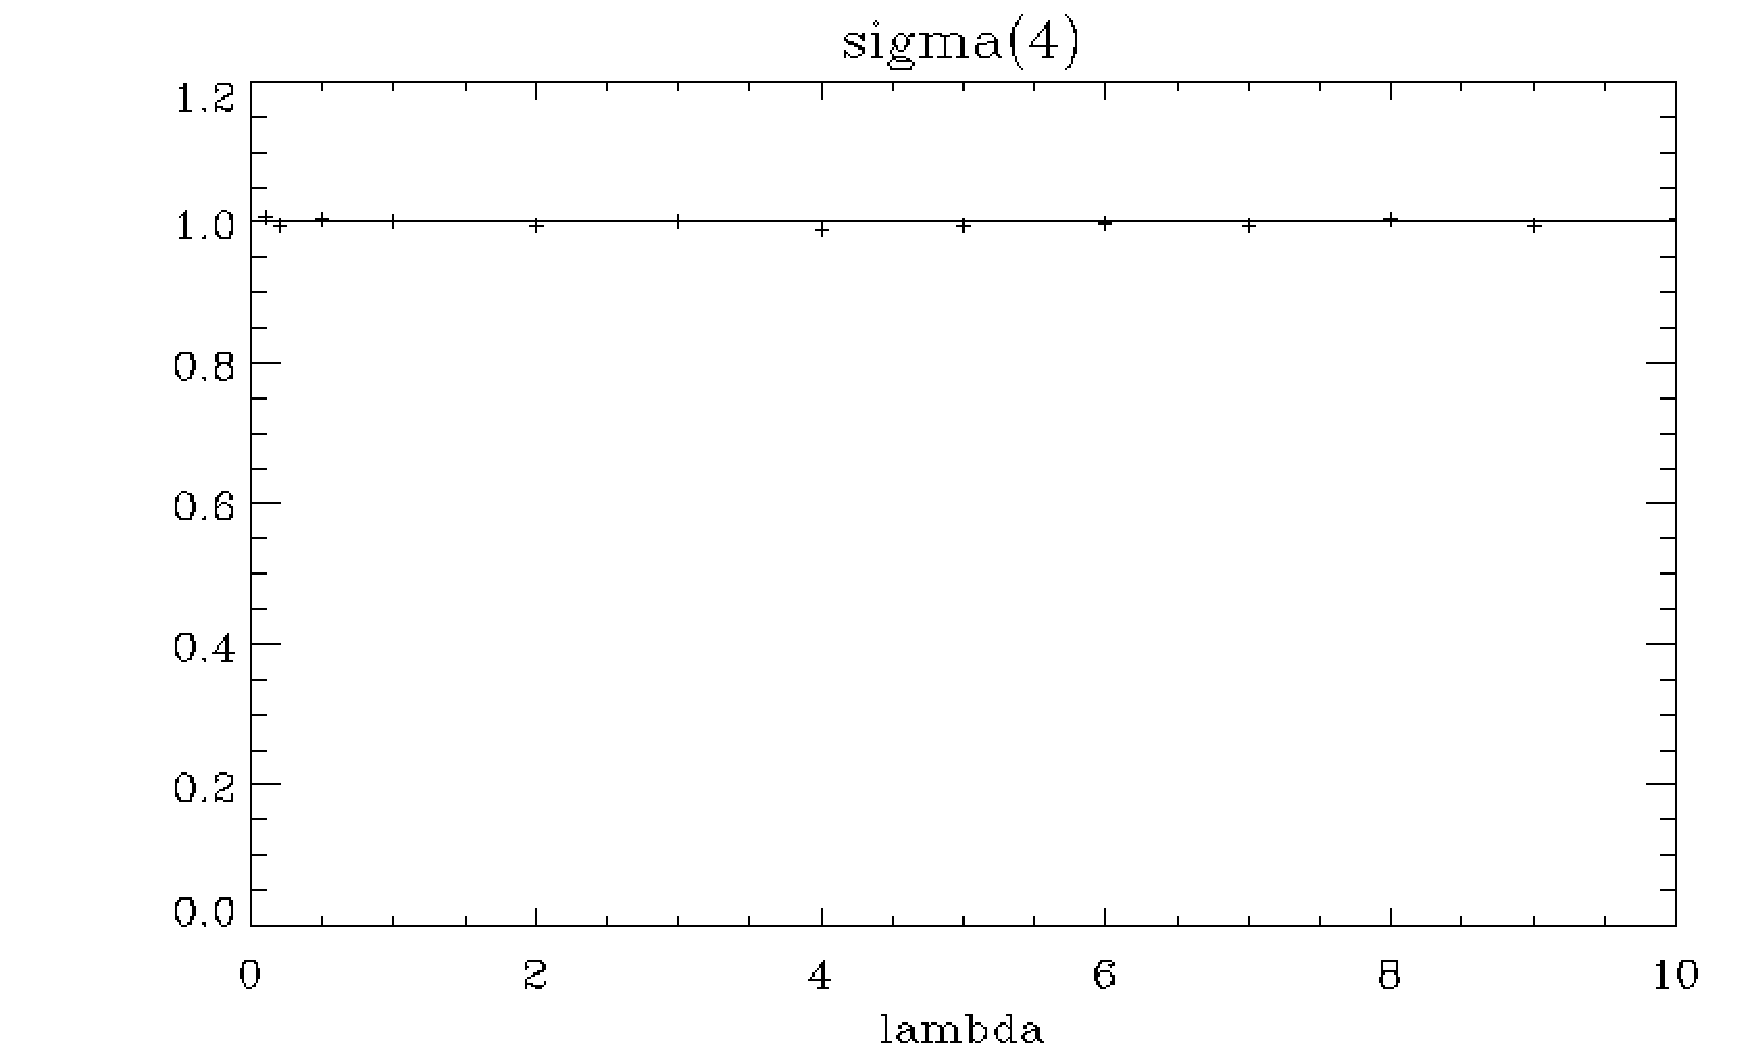
\includegraphics[width=2.5in, height=3in]{13822fg4.pdf}
}}
\caption{Normalized value ($\mathbf{ (\sigma_{(j)})_{\text{simulated}} }/ (\sigma_{(j)})_{\text{theoretical}}$) of the stabilized variances at each scale $j$ as a function of $\lambda$.}
\label{sigma}
\end{figure}

\begin{figure}[htb]
\centering
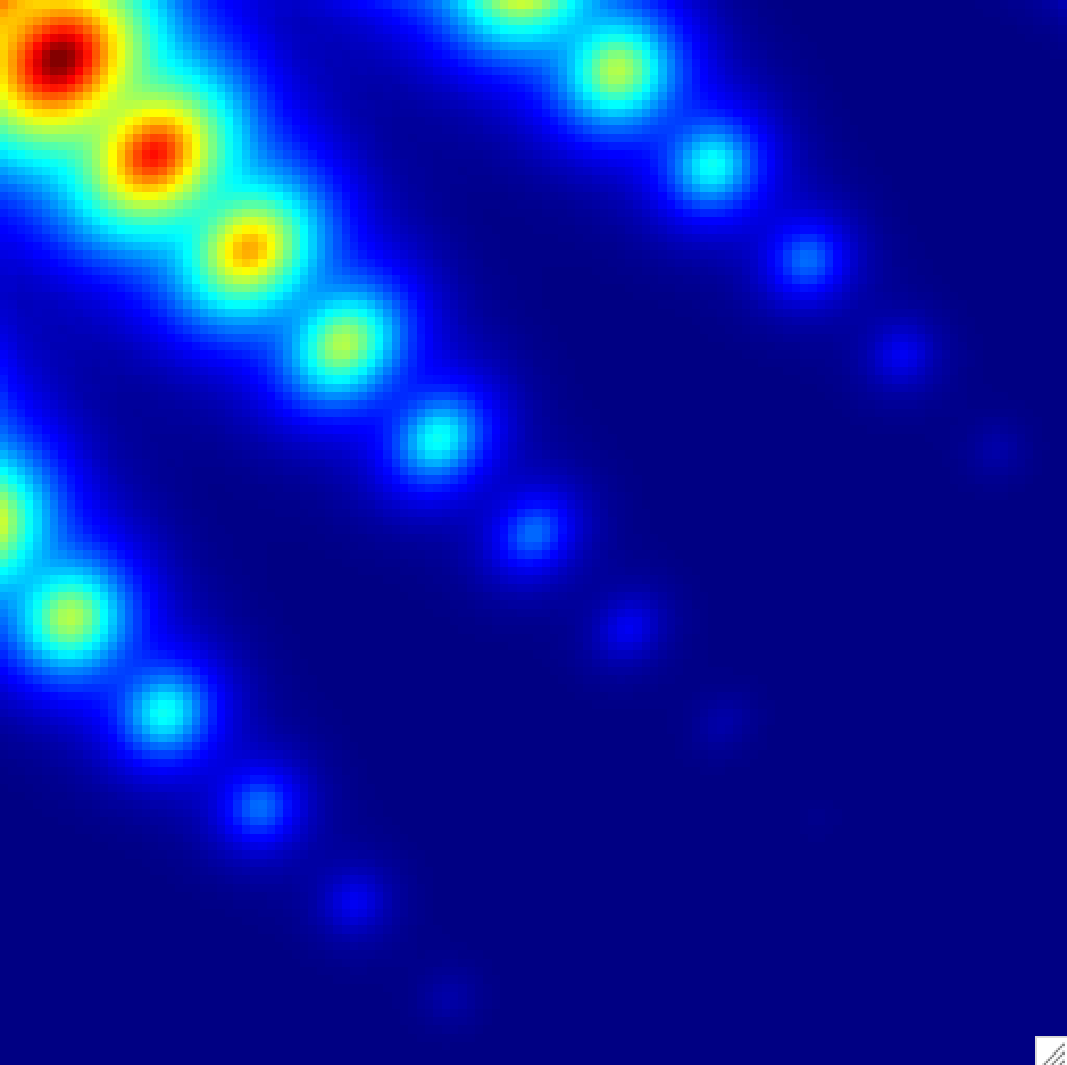
\includegraphics[width=2.5in]{13822fg6.pdf}
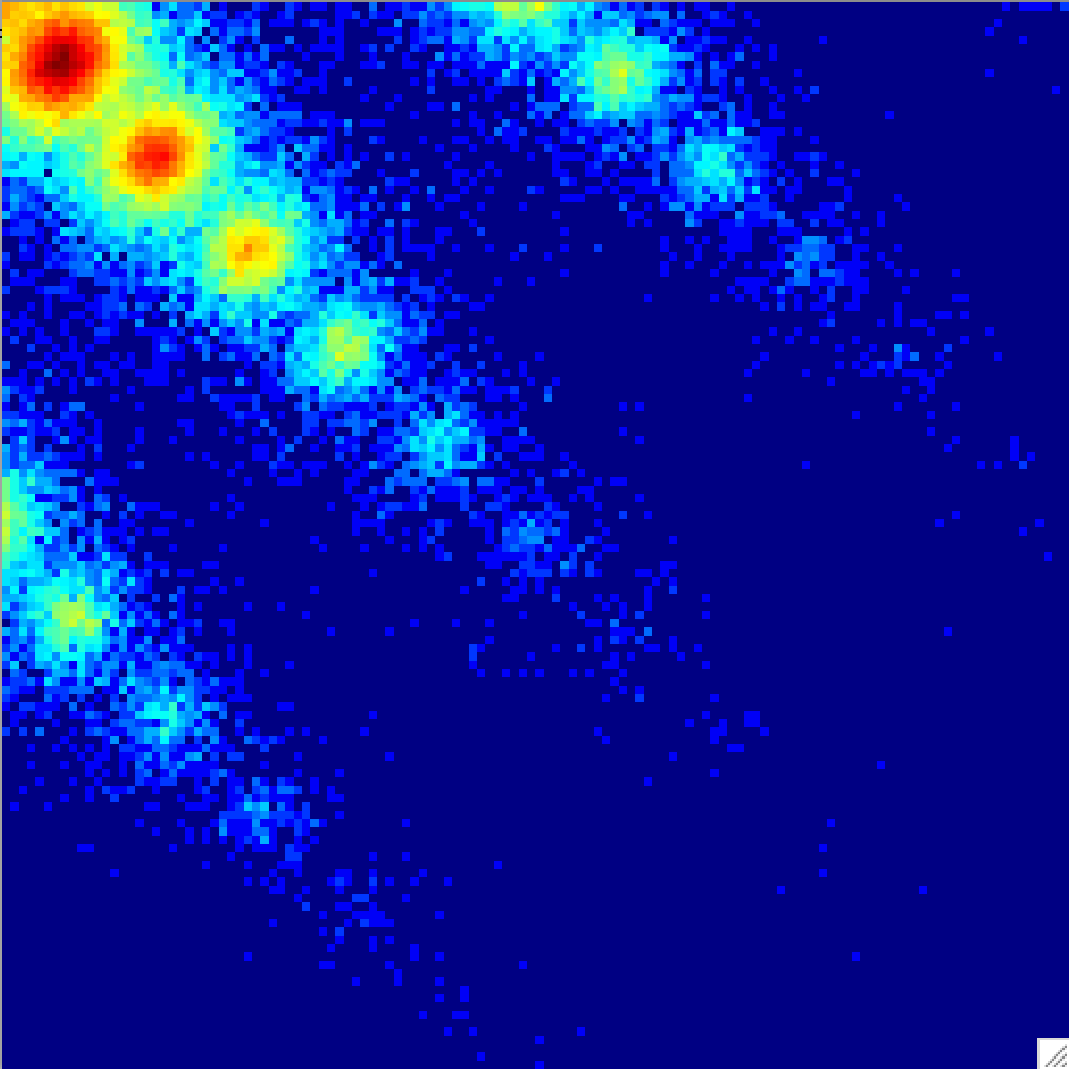
\includegraphics[width=2.5in]{13822fg7.pdf}
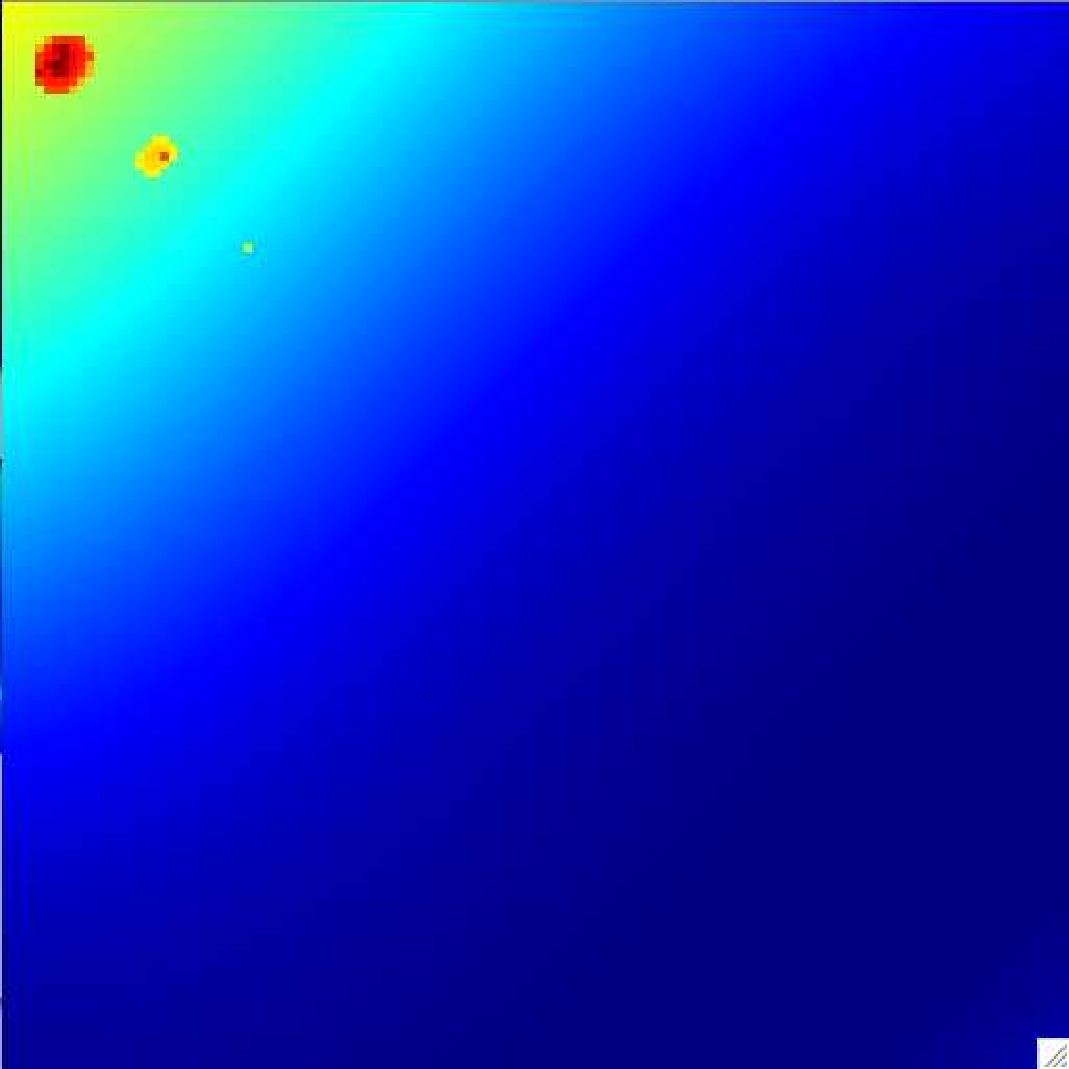
\includegraphics[width=2.5in]{13822fg8.pdf}
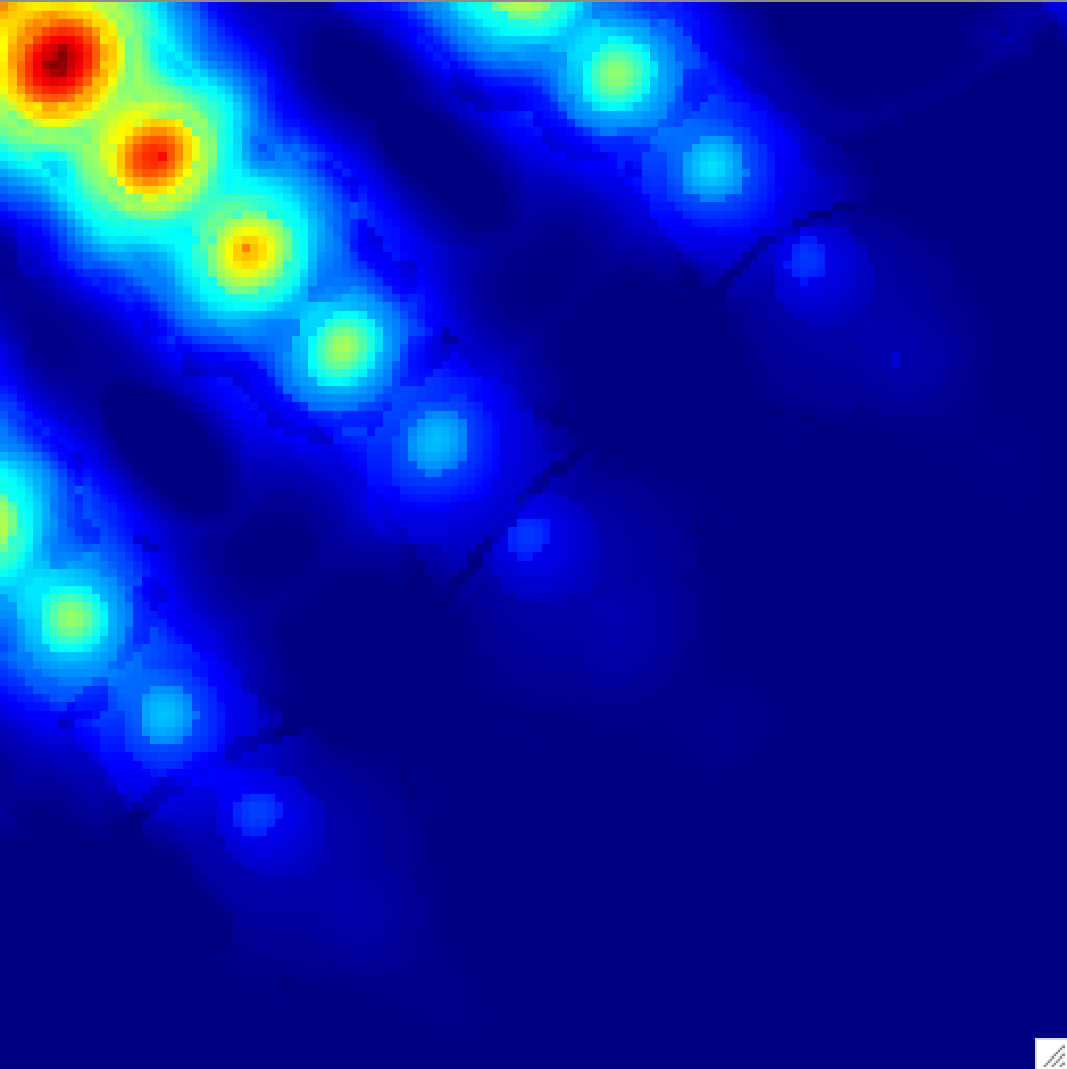
\includegraphics[width=2.5in]{13822fg9.pdf}
\caption{Comparison of MS-VSTS with Anscombe + wavelet shrinkage on a single HEALPix face.
\emph{Top Left} : Sources of varying intensity.
\emph{Top Right} : Sources of varying intensity with Poisson noise.
\emph{Bottom Left} : Poisson sources of varying intensity reconstructed with Anscombe + wavelet shrinkage.
\emph{Bottom Right} : Poisson sources of varying intensity reconstructed with MS-VSTS.
}
\label{ansc}
\end{figure}

\subsection{MS-VSTS + Curvelets}

As the first step of the algorithm is an IUWT, we can stabilize each resolution level as in Equation~(\ref{eq27}). We then apply the local ridgelet transform on each stabilized wavelet band.

It is not as straightforward as with the IUWT to derive the asymptotic noise variance in the stabilized curvelet domain. In our experiments, we derived them using simulated Poisson data of stationary intensity level $\lambda$. After having checked that the standard deviation in the curvelet bands becomes stabilized as the intensity level increases (which means that the stabilization is working properly), we stored the standard deviation $\sigma_{j,l}$ for each wavelet scale $j$ and each ridgelet band $l$ (Table~\ref{tabcurv}).

\begin{table*}[!h]
  \centering
   \caption{Asymptotic values of the variances $\sigma_{j,k}$ of the curvelet coefficients.
  }
  \begin{tabular}{|c|c|c|c|c|}
\hline
 $j$ & $l=1$ & $l=2$ & $l=3$ & $l=4$ \\
\hline
  1 & 1.74550 & 0.348175 & & \\
  2 & 0.230621 & 0.248233 & 0.196981 & \\
  3 & 0.0548140 & 0.0989918 & 0.219056 & \\
  4 & 0.0212912 & 0.0417454 & 0.0875663 & 0.20375 \\
  5 & 0.00989616 & 0.0158273 & 0.0352021 & 0.163248 \\
\hline
\end{tabular}
 
  \label{tabcurv}
\end{table*}
  
\chapter{Poisson denoising}
\label{ch_denoising}

\markright{Poisson denoising}

\section{MS-VST + IUWT}

Under the hypothesis of homogeneous Poisson intensity, the stabilized wavelet coefficients $d_j$ behave like centered Gaussian variables of standard deviation $\sigma_{(j)}$. We can detect significant coefficients with binary hypothesis testing as in Gaussian denoising.

Under the null hypothesis $\mathcal{H}_0$ of homogeneous Poisson intensity, the distribution of the stabilized wavelet coefficient $d_j[k]$ at scale $j$ and location index $k$ can be written as:
\begin{equation}
\label{ }
p(d_j[k]) = \frac{1}{\sqrt{2\pi}\sigma_j}\exp(-d_j[k]^2 / 2 \sigma_j^2) .
\end{equation}

The rejection of the hypothesis $\mathcal{H}_0$ depends on the double-sided p-value:
\begin{equation}
\label{ }
p_j[k] = 2 \frac{1}{\sqrt{2\pi}\sigma_j}\int_{|d_j[k]|}^{+\infty} \exp(-x^2 / 2 \sigma_j^2) dx .
\end{equation}

Consequently, to accept or reject $\mathcal{H}_0$, we compare each $|d_j[k]|$ with a critical threshold $\kappa \sigma_j$, $\kappa= 3,4 \text{ or } 5$ corresponding respectively to significance levels. This amounts to deciding that:
\begin{itemize}
  \item if $|d_j[k]| \geqslant  \kappa \sigma_j$, $d_j[k]$ is significant.
  \item if $|d_j[k]| < \kappa \sigma_j$, $d_j[k]$ is not significant.
\end{itemize}

Then we have to invert the MS-VSTS scheme to reconstruct the estimate. However, although the direct inversion is possible (Eq. (\ref{eq30})), it can not guarantee a positive intensity estimate, while the Poisson intensity is always nonnegative. A positivity projection can be applied, but important structures could be lost in the estimate. To tackle this problem, we reformulate the reconstruction as a convex optimisation problem and solve it iteratively with an algorithm based on Hybrid Steepest Descent (HSD)~\citep{wave:yamada01}.

We define the multiresolution support $\mathcal{M}$, which is determined by the set of detected significant coefficients after hypothesis testing:
\begin{equation}
\label{eq33}
\mathcal{M} := \{ (j,k) | \text{if } d_j[k] \text{ is declared significant} \} .
\end{equation}

We formulate the reconstruction problem as a convex constrained minimization problem:

\begin{equation}
\label{eq34}
\begin{split}
\text{Arg} \min_{\mathbf{X}} \| \mathbf{ \Phi}^{T}\mathbf{X}\|_1,
\text{s.t.} \\ \: \left\{\begin{array}{c}\mathbf{X} \geqslant 0 , \\\forall (j,k)\in \mathcal{M},      (\mathbf{ \Phi}^{T}\mathbf{X})_j[k]=(\mathbf{ \Phi}^{T}\mathbf{Y})_j[k] , \end{array}\right.
\end{split}
\end{equation}
where $\mathbf{\Phi}$ denotes the IUWT synthesis operator.

This problem is solved with the following iterative scheme: the image is initialised by $\mathbf{X}^{(0)} = 0$, and the iteration scheme is, for $n=0$ to $N_{\max}-1$:


\begin{eqnarray}
\tilde{\mathbf{X}} &=& P_{+}[\mathbf{ X}^{(n)} + \mathbf{ \Phi} P_{\mathcal{M}} \mathbf{ \Phi}^{T} (\mathbf{ Y} - \mathbf{ X}^{(n)})] \\
\mathbf{X}^{(n+1)} &=& \mathbf{ \Phi}\text{ST}_{\lambda_n}[\mathbf{ \Phi}^{T}\tilde{\mathbf{X}}]
\end{eqnarray}
where $P_{+}$ denotes the projection on the positive orthant, $P_{\mathcal{M}}$ denotes the projection on the multiresolution support $\mathcal{M}$:
\begin{equation}
P_{\mathcal{M}}d_j[k] = \left\{\begin{array}{cc} d_j[k] & \text{if} \  (j,k) \in \mathcal{M} , \\0 & \text{otherwise} \end{array} . \right.
\end{equation}
and $\text{ST}_{\lambda_n}$ the soft-thresholding with threshold $\lambda_n$:
\begin{equation}
\text{ST}_{\lambda_n} [d] = \left\{\begin{array}{cc} \mathrm{sign}(d)(|d| - \lambda_n) & \text{if} \ |d| \geqslant \lambda_n , \\0 & \text{otherwise} \end{array} . \right.
\end{equation}
We chose a decreasing threshold $\lambda_n = \frac{N_{\max} - n}{N_{\max} - 1},n=1,2,\cdots,N_{\max}$.

The final estimate of the Poisson intensity is: $\hat{\mathbf{\Lambda}} = \mathbf{X}^{(N_{\max})}$. Algorithm~\ref{alg1} summarizes the main steps of the MS-VSTS + IUWT denoising algorithm.



\begin{algorithm}[!h]
\caption{MS-VSTS + IUWT Denoising}
\label{alg1}
\begin{algorithmic}[1]
\REQUIRE $\quad$ data $a_0:=\mathbf{Y}$, number of iterations $N_{\max}$, threshold $\kappa$ \\
\underline{\emph{\textbf{Detection}}} \\
\FOR{$j=1$ to $J$}
\STATE Compute $a_j$ and $d_j$ using (\ref{eq27}).
\STATE Hard threshold $|d_j[k]|$ with threshold $\kappa \sigma_j$ and update $\mathcal{M}$.
\ENDFOR \\
\underline{\emph{\textbf{Estimation}}} \\
\STATE Initialize $\mathbf{X}^{(0)}=0$, $\lambda_0 = 1$.
\FOR{$n=0$ to $N_{\max}-1$}
\STATE $\tilde{\mathbf{X}}= P_{+}[\mathbf{ X}^{(n)} + \mathbf{ \Phi} P_{\mathcal{M}} \mathbf{ \Phi}^{T} (\mathbf{ Y} - \mathbf{ X}^{(n)})]$.
\STATE $\mathbf{X}^{(n+1)} = \mathbf{ \Phi}\text{ST}_{\lambda_n}[\mathbf{ \Phi}^{T}\tilde{\mathbf{X}}]$.
\STATE $\lambda_{n+1} = \frac{N_{\max} - (n+1)}{N_{\max} - 1}$.
\ENDFOR
\STATE Get the estimate $\hat{\mathbf{\Lambda}} = \mathbf{X}^{(N_{\max})}$.

\end{algorithmic}
\end{algorithm}


\section{Multi-resolution support adaptation}

When two sources are too close, the less intense source may not be detected because of the negative wavelet coefficients of the brightest source. To avoid such a drawback, we may update the multi-resolution support at each iteration. The idea is to withdraw the detected sources and to make a detection on the remaining residual, so as to detect the sources which may have been missed at the first detection.


At each iteration $n$, we compute the MS-VSTS of $\mathbf{X}^{(n)}$. We denote $d^{(n)}_j[k]$ the stabilised coefficients of $\mathbf{X}^{(n)}$. We make a hard thresholding on $(d_j[k]-d^{(n)}_j[k])$ with the same thresholds as in the detection step. Significant coefficients are added to the multiresolution support $\mathcal{M}$.

\begin{algorithm}
\caption{MS-VSTS + IUWT Denoising + Multiresolution Support Adaptation}
\label{alg4}
\begin{algorithmic}[1]
\REQUIRE $\quad$ data $a_0:=\mathbf{Y}$, number of iterations $N_{\max}$, threshold $\kappa$ \\
\underline{\emph{\textbf{Detection}}} \\
\FOR{$j=1$ to $J$}
\STATE Compute $a_j$ and $d_j$ using (\ref{eq27}).
\STATE Hard threshold $|d_j[k]|$ with threshold $\kappa \sigma_j$ and update $\mathcal{M}$.
\ENDFOR \\
\underline{\emph{\textbf{Estimation}}} \\
\STATE Initialize $\mathbf{X}^{(0)}=0$, $\lambda_0 = 1$.
\FOR{$n=0$ to $N_{\max}-1$}
\STATE $\tilde{\mathbf{X}}= P_{+}[\mathbf{ X}^{(n)} + \mathbf{ \Phi} P_{\mathcal{M}} \mathbf{ \Phi}^{T} (\mathbf{ Y} - \mathbf{ X}^{(n)})]$.
\STATE $\mathbf{X}^{(n+1)} = \mathbf{ \Phi}\text{ST}_{\lambda_n}[\mathbf{ \Phi}^{T}\tilde{\mathbf{X}}]$.
\STATE Compute the MS-VSTS on  $\mathbf{X}^{(n)}$ to get the stabilised coeffcients $d^{(n)}_j$.
\STATE Hard threshold $|d_j[k]-d^{(n)}_j[k]|$ and update $\mathcal{M}$.
\STATE $\lambda_{n+1} = \frac{N_{\max} - (n+1)}{N_{\max} - 1}$.
\ENDFOR
\STATE Get the estimate $\hat{\mathbf{\Lambda}} = \mathbf{X}^{(N_{\max})}$.

\end{algorithmic}
\end{algorithm}

The main steps of the algorithm are summarized in Algorithm~\ref{alg4}. In practice, we use Algorithm~\ref{alg4} instead of Algorithm~\ref{alg1} in our experiments.

\section{MS-VST + Curvelets}

Insignificant coefficients are zeroed by using the same hypothesis testing framework as in the wavelet scale. At each wavelet scale $j$ and ridgelet band $k$, we make a hard thresholding on curvelet coefficients with threshold $\kappa \sigma_{j,k}$, $\kappa= 3,4 \text{ or } 5$. Finally, a direct reconstruction can be performed by first inverting the local ridgelet transforms and then inverting the MS-VST + IUWT~(Equation~(\ref{eq30})). An iterative reconstruction may also be performed.

Algorithm~\ref{algcurv} summarizes the  main steps of the MS-VSTS + Curvelets denoising algorithm.

\begin{algorithm}
\caption{MS-VSTS + Curvelets Denoising}
\label{algcurv}
\begin{algorithmic}[1]
\STATE Apply the MS-VST + IUWT with $J$ scales to get the stabilized wavelet subbands $d_j$.
\STATE Set $B_1 = B_{\min}$.
\FOR{$j=1$ to $J$}
\STATE Partition the subband $d_j$ with blocks of side-length $B_j$ and apply the digital ridgelet transform to each block to obtain the stabilized curvelets coefficients.
\IF {$j$ modulo $2=1$}
\STATE $B_{j+1} = 2 B_j$
\ELSE
\STATE $B_{j+1} =  B_j$
\ENDIF \\
\STATE HTs on the stabilized curvelet coefficients.
\ENDFOR \\
\STATE Invert the ridgelet transform in each block before inverting the MS-VST + IUWT.

\end{algorithmic}
\end{algorithm}


\section{Experiments}

The method was tested on simulated Fermi data. The simulated data are the sum of a Milky Way diffuse background model and 1000 gamma ray point sources. We based our Galactic diffuse emission model intensity on the model $gll\_iem\_v02$ obtained at the Fermi Science Support Center~\citep{Models}
. This model results from a fit of the LAT photons with various gas templates as well as inverse Compton in several energy bands. We used a realistic point-spread function for the sources, based on Monte Carlo simulations of the LAT and accelerator tests, that scale approximately as $0.8(E/1GeV)^{-0.8}$ degrees. The position of the 205 brightest sources were taken from the Fermi 3-month source list~\citep{Abdo}. The position of the 795 remaining sources follow the LAT 1-year Point Source Catalog~\citep{Catalog}
  sources distribution: each simulated source was randomly sorted in a box of $\Delta$l=5$^o$ and $\Delta$b=1$^o$ around a LAT 1-year catalog source. We simulated each source assuming a power-law dependence with its spectral index given by the 3-month source list and the first year catalog. We used an exposure of $3.10^{10} s.cm^2$ corresponding approximatively to one year of Fermi all-sky survey around 1 GeV. The simulated counts map shown here correspond to photons energy from 150 MeV to 20 GeV.


Fig.~\ref{rechsd} compares the result of denoising with MS-VST + IUWT (Algorithm~\ref{alg1}), MS-VST + curvelets (Algorithm~\ref{algcurv}) and Anscombe VST + wavelet shrinkage on a simulated Fermi map. Fig.~\ref{recface} shows one HEALPix face of the results. 
As expected from theory, the Anscombe method produces poor results to  denoise Fermi data, because the underlyning intensity is too weak. 
Both wavelet and curvelet denoising on the sphere  perform much better. 
For this application, wavelets are slightly better than curvelets ($SNR_{wavelets} = 65.8 dB$, $SNR_{curvelets} = 37.3 dB$, $SNR (dB) = 20 \log (\sigma_{signal} / \sigma_{noise})$). As this image contains many point sources, thisresult is expected. Indeed wavelet are better than curvelets to represent isotropic objects.

\begin{figure}[htb]
\centering{
\hbox{
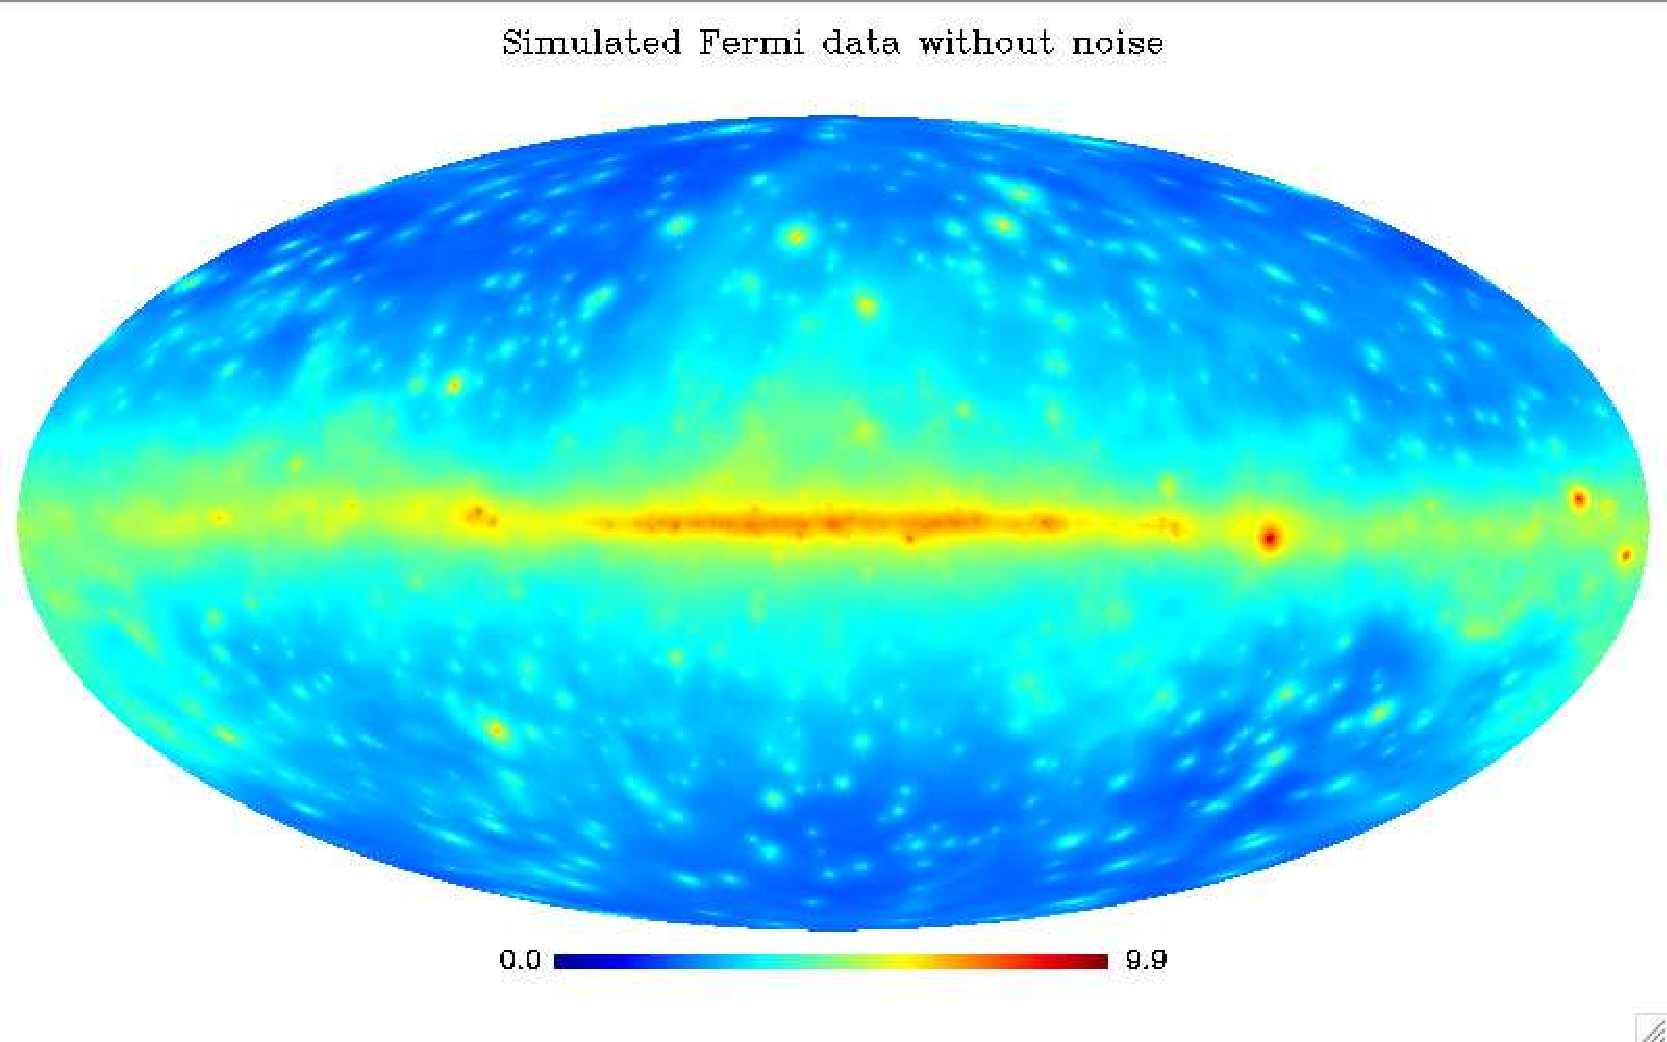
\includegraphics[width=3in,height=2.4in]{13822fg10.pdf}  
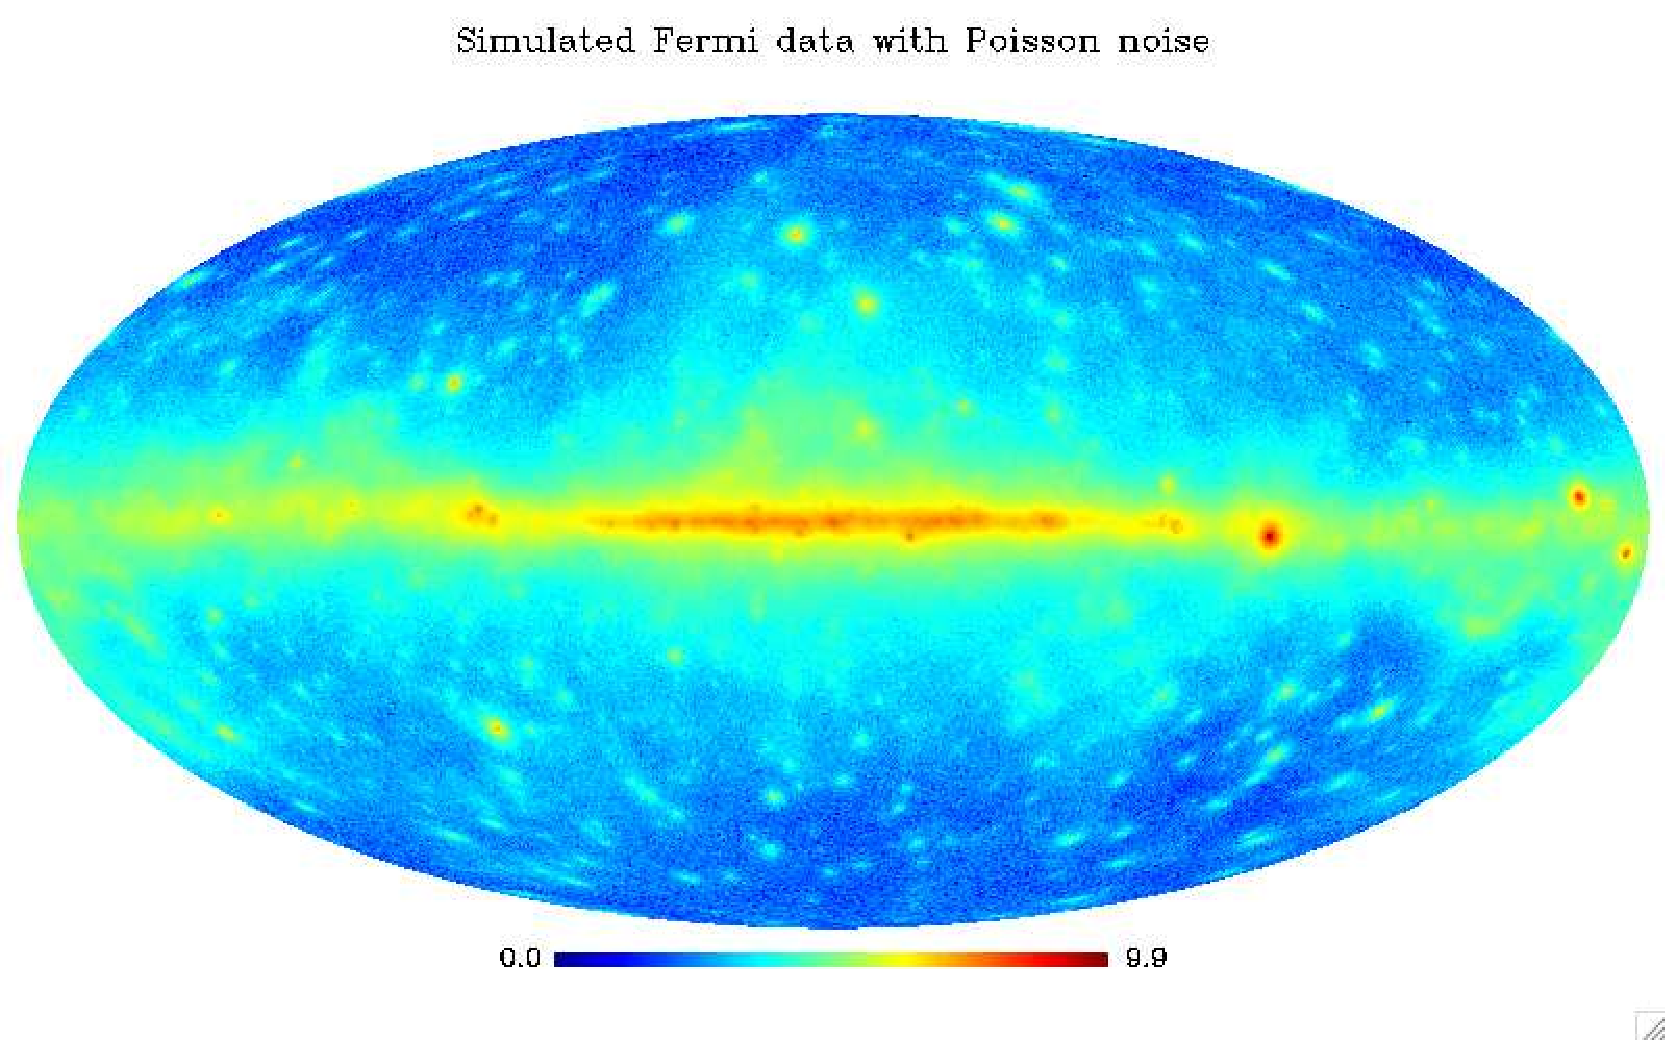
\includegraphics[width=3in,height=2.4in]{13822fg11.pdf}} 
\hbox{
\includegraphics[width=3in,height=2.4in]{13822fg12.pdf} 
\includegraphics[width=3in,height=2.4in]{13822fg13.pdf}}
\hbox{
\includegraphics[width=3in,height=2.4in]{13822fg14.pdf} 
\includegraphics[width=3in,height=2.4in]{13822fg15.pdf}}

\caption{\emph{Top Left}: Fermi simulated map without noise.
\emph{Top Right}: Fermi simulated map with Poisson noise.
\emph{Middle Left}: Fermi simulated map denoised with Anscombe VST + wavelet shrinkage.
\emph{Middle Right}: Fermi simulated map denoised with MS-VSTS + curvelets (Algorithm~\ref{algcurv}).
\emph{Bottom Left}: Fermi simulated map denoised with MS-VSTS + IUWT (Algorithm~\ref{alg1}) with threshold $5\sigma_j$.
\emph{Bottom Right}: Fermi simulated map denoised with MS-VSTS + IUWT (Algorithm~\ref{alg1}) with threshold $3\sigma_j$.
Pictures are in logarithmic scale.}
\label{rechsd}
}
\end{figure}

\begin{figure*}
\begin{center}
\includegraphics[width=2.5in]{13822fg16.pdf} \hfill
\includegraphics[width=2.5in]{13822fg17.pdf} \hfill
\includegraphics[width=2.5in]{13822fg18.pdf} \hfill
\includegraphics[width=2.5in]{13822fg19.pdf} \hfill
\includegraphics[width=2.5in]{13822fg20.pdf} \hfill
\includegraphics[width=2.5in]{13822fg21.pdf} \hfill
\caption{View of a single HEALPix face from the results of Figure~\ref{rechsd}.
\emph{Top Left}: Fermi simulated map without noise.
\emph{Top Right}: Fermi simulated map with Poisson noise.
\emph{Middle Left}: Fermi simulated map denoised with Anscombe VST + wavelet shrinkage.
\emph{Middle Right}: Fermi simulated map denoised with MS-VSTS + curvelets (Algorithm~\ref{algcurv}).
\emph{Bottom Left}: Fermi simulated map denoised with MS-VSTS + IUWT (Algorithm~\ref{alg1}) with threshold $5\sigma_j$.
\emph{Bottom Right}: Fermi simulated map denoised with MS-VSTS + IUWT (Algorithm~\ref{alg1}) with threshold $3\sigma_j$.
Pictures are in logarithmic scale.
}
\label{recface}
\end{center}
\end{figure*}
  
\chapter{Milky Way diffuse background study: denoising and inpainting}
\label{ch_inpainting}

% \markright{Milky Way diffuse background study: denoising and inpainting}

In order to extract a  diffuse emission, we want to remove the  point sources from the data. 
As our HSD algorithm is very close to the MCA algorithm~\citep{starck:sta04}, an idea is to mask the most intense sources and to modify our algorithm in order to interpolate through the gaps exactly as in the MCA-Inpainting algorithm~\citep{inpainting:abrial06}. 
This modified algorithm can be called MS-VSTS-Inpainting algorithm.

The problem can be reformulated as a convex constrained minimization problem:

\begin{equation}
\label{inp_eq34}
\begin{split}
\text{Arg} \min_{\mathbf{X}} \| \mathbf{ \Phi}^{T}\mathbf{X}\|_1,
\text{s.t.} \\ \: \left\{\begin{array}{c}\mathbf{X} \geqslant 0 , \\\forall (j,k)\in \mathcal{M},      (\mathbf{ \Phi}^{T}\Pi \mathbf{X})_j[k]=(\mathbf{ \Phi}^{T} \mathbf{Y})_j[k] , \end{array}\right. 
\end{split}
\end{equation}
where $\Pi$ is a binary mask ($1$ on valid data and $0$ on invalid data).

The iterative scheme can be adapted to cope with a binary mask, which gives:
\begin{eqnarray}
\tilde{\mathbf{X}} = P_{+}[\mathbf{ X}^{(n)} + \mathbf{ \Phi} P_{\mathcal{M}} \mathbf{ \Phi}^{T} \Pi (\mathbf{ Y} - \mathbf{ X}^{(n)})] , \\
\mathbf{X}^{(n+1)} = \mathbf{ \Phi} \text{ST}_{\lambda_n}[\mathbf{ \Phi}\tilde{\mathbf{X}}] .
\end{eqnarray}


The thresholding strategy has to be adapted. Indeed, for the impainting task we need to have a very large initial threshold in order to have a very smooth image in the beginning and to refine the details progressively. We chose an exponentially decreasing threshold:
\begin{equation}
\label{eq42}
\lambda_{n} = \lambda_{\max}  (2^{(\frac{N_{\max} - n}{N_{\max} - 1})} -1),n=1,2,\cdots,N_{\max} ,
\end{equation}
where $\lambda_{\max} = \max (\mathbf{\Phi}^{T}\mathbf{X})$.

\begin{algorithm}
\caption{MS-VST + IUWT Denoising + Inpainting}
\label{alg2}

\begin{algorithmic}[1]
\REQUIRE $\quad$ data $a_0:=\mathbf{Y}$, mask $\Pi$, number of iterations $N_{\max}$, threshold $\kappa$.\\
\underline{\emph{\textbf{Detection}}} \\
\FOR{$j=1$ to $J$}
\STATE Compute $a_j$ and $d_j$ using (\ref{eq27}).
\STATE Hard threshold $|d_j[k]|$ with threshold $\kappa \sigma_j$ and update $\mathcal{M}$.
\ENDFOR \\
\underline{\emph{\textbf{Estimation}}} \\
\STATE Initialize $\mathbf{X}^{(0)}=0$, $\lambda_{0} = \lambda_{\max}$.
\FOR{$n=0$ to $N_{\max}-1$}
\STATE $\tilde{\mathbf{X}}= P_{+}[\mathbf{ X}^{(n)} + \mathbf{ \Phi} P_{\mathcal{M}} \mathbf{ \Phi}^{T} \Pi(\mathbf{ Y} - \mathbf{ X}^{(n)})]$.
\STATE $\mathbf{X}^{(n+1)} = \mathbf{ \Phi}^\text{ST}_{\lambda_n}[\mathbf{ \Phi}^{T}\tilde{\mathbf{X}}]$.
\STATE $\lambda_{n+1} = \lambda_{\max}  (2^{(\frac{N_{\max} - (n+1)}{N_{\max} - 1})} -1)$
\ENDFOR
\STATE Get the estimate $\hat{\mathbf{\Lambda}} = \mathbf{X}^{(N_{\max})}$.

\end{algorithmic}
\end{algorithm}



\section*{Experiment}

We applied this method on simulated Fermi data where we masked the most luminous sources.

The results are on Figure~\ref{impainting}. The MS-VST + IUWT + Inpainting method (Algorithm~\ref{alg2}) interpolates the missing data very well. Indeed, the missing part can not be seen anymore in the inpainted map, which shows that the diffuse emission component  has been correctly reconstructed.


\begin{figure}[htb]
\centering{
\includegraphics[width=5.5in]{13822fg22.pdf} 
\includegraphics[width=5.5in]{13822fg23.pdf} 
}
\caption{MS-VSTS - Inpainting.
\emph{Top}: Fermi simulated map with Poisson noise and the most luminous sources masked.
\emph{Bottomt}: Fermi simulated map denoised and inpainted with wavelets (Algorithm~\ref{alg2}).
Pictures are in logarithmic scale.
}
\label{impainting}
\end{figure}
  
\chapter{Source detection: denoising and background modeling}
\label{ch_background}

% \markright{Source detection: denoising and background modeling}

\section{Method}
In some cases such as for Fermi data, the diffuse emission from the Milky Way  makes a relatively intense background. We have to extract this background in order to detect point sources. This diffuse interstellar emission may be modeled, and we want to use such a background model and incorporate a background removal in our denoising algorithm.

We note $\mathbf{Y}$ the data, $\mathbf{B}$ the background we want to remove, and $d^{(b)}_{j}[k]$ the MS-VSTS coefficients of $\mathbf{B}$ at scale $j$ and position $k$. We determine the multi-resolution support by comparing $|d_j[k]-d^{(b)}_{j}[k]|$ with $\kappa \sigma_j$.

We formulate the reconstruction problem as a convex constrained minimization problem:

\begin{equation}
\label{bgr_eq34}
\begin{split}
\text{Arg} \min_{\mathbf{X}} \| \mathbf{ \Phi}^{T}\mathbf{X}\|_1,
\text{s.t.} \\ \: \left\{\begin{array}{c}\mathbf{X} \geqslant 0 , \\\forall (j,k)\in \mathcal{M},      (\mathbf{ \Phi}^{T}\mathbf{X})_j[k]=(\mathbf{ \Phi}^{T}(\mathbf{Y} - \mathbf{B}))_j[k] , \end{array}\right.
\end{split}
\end{equation}

Then, the reconstruction algorithm scheme becomes:
\begin{eqnarray}
\tilde{\mathbf{X}} = P_{+}[\mathbf{ X}^{(n)} + \mathbf{ \Phi} P_{\mathcal{M}} \mathbf{ \Phi}^{T} (\mathbf{ Y} - \mathbf{B} - \mathbf{ X}^{(n)})] , \\
\mathbf{X}^{(n+1)} = \mathbf{ \Phi}\text{ST}_{\lambda_n}[\mathbf{ \Phi}^{T}\tilde{\mathbf{X}}].
\end{eqnarray}

\begin{figure}[htb]
\begin{center}
\includegraphics[width=2.9in]{13822fg24.pdf} \hfill
\includegraphics[width=2.9in]{13822fg25.pdf} \hfill
\includegraphics[width=2.9in]{13822fg26.pdf} \hfill
\includegraphics[width=2.9in]{13822fg27.pdf}
\caption{Theoretical testing for MS-VSTS + IUWT denoising + background removal algorithm (Algorithm~\ref{alg3}). View on a single HEALPix face.
\emph{Top Left}: Simulated background : sum of two Gaussians of standard deviation equal to 0.1 and 0.01 respectively.
\emph{Top Right}: Simulated source: Gaussian of standard deviation equal to 0.01.
\emph{Bottom Left}: Simulated poisson data.
\emph{Bottom Right}: Image denoised with MS-VSTS + IUWT and background removal.
}
\label{background}
\end{center}
\end{figure}
The algorithm is illustrated by the theoretical study in Figure~\ref{background}. We denoise Poisson data while separating a single source, which is a Gaussian of standard deviation equal to 0.01, from a background, which is a sum of two Gaussians of standard deviation equal to 0.1 and 0.01 respectively. 

\begin{algorithm}
\caption{MS-VSTS + IUWT Denoising + Background extraction}
\label{alg3}

\begin{algorithmic}[1]
\REQUIRE $\quad$ data $a_0:=\mathbf{Y}$, background $B$, number of iterations $N_{\max}$, threshold $\kappa$. \\
\underline{\emph{\textbf{Detection}}} \\
\FOR{$j=1$ to $J$}
\STATE Compute $a_j$ and $d_j$ using (\ref{eq27}).
\STATE Hard threshold $(d_j[k] - d^{(b)}_{j}[k])$ with threshold $\kappa \sigma_j$ and update $\mathcal{M}$.
\ENDFOR \\
\underline{\emph{\textbf{Estimation}}} \\
\STATE Initialize $\mathbf{X}^{(0)}=0$, $\lambda_0 = 1$.
\FOR{$n=0$ to $N_{\max}-1$}
\STATE $\tilde{\mathbf{X}}= P_{+}[\mathbf{ X}^{(n)} + \mathbf{ \Phi} P_{\mathcal{M}} \mathbf{ \Phi}^{T} (\mathbf{ Y} - \mathbf{B} - \mathbf{ X}^{(n)})]$.
\STATE $\mathbf{X}^{(n+1)} = \mathbf{ \Phi}\text{ST}_{\lambda_n}[\mathbf{ \Phi}^{T}\tilde{\mathbf{X}}]$.
\STATE $\lambda_{n+1} = \frac{N_{\max} - (n+1)}{N_{\max} - 1}$.
\ENDFOR
\STATE Get the estimate $\hat{\mathbf{\Lambda}} = \mathbf{X}^{(N_{\max})}$.
\end{algorithmic}
\end{algorithm}

Like Algorithm~\ref{alg1}, Algorithm~\ref{alg3} can be adapted to make multiresolution support adaptation.


\section{Experiment}

We applied Algorithms~\ref{alg3} on simulated Fermi data. To test the efficiency of our method, we detect the sources with the SExtractor routine~\citep{astro:bertin96}, and compare the detected sources with the theoretical sources catalog to get the number of true and false detections. Results are shown on Figures~\ref{sources} and~\ref{sourcesreest}. The SExtractor method was applied on the first wavelet scale of the reconstructed map, with a detection threshold equal to 1. It has been chosen to optimise the number of true detections. SExtractor makes $593$ true detections and $71$ false detections on the Fermi simulated map restored with Algorithm~\ref{alg4} among the $1000$ sources of the simulation. On noisy data, many fluctuations due to Poisson noise are detected as sources by SExtractor, which leads to a big number of false detections (more than 2000 in the case of Fermi data). 

\begin{figure}[htb]
\begin{center}
\includegraphics[width=2.9in]{13822fg28.pdf} \hfill
\includegraphics[width=2.9in]{13822fg29.pdf} \hfill
\includegraphics[width=2.9in]{13822fg30.pdf} \hfill
\includegraphics[width=2.9in]{13822fg31.pdf} \hfill
\includegraphics[width=2.9in]{13822fg32.pdf}
\caption{\emph{Top Left}: Simulated background model.
\emph{Top Right}: Simulated Gamma Ray sources.
\emph{Middle Left}: Simulated Fermi data with Poisson noise.
\emph{Middle Right}: Reconstructed Gamma Ray Sources with MS-VSTS + IUWT + background removal (Algorithm~\ref{alg3}) with threshold $5\sigma_j$.
\emph{Bottom}: Reconstructed Gamma Ray Sources with MS-VSTS + IUWT + background removal (Algorithm~\ref{alg3}) with threshold $3\sigma_j$.
Pictures are in logarithmic scale.}
\label{sources}
\end{center}
\end{figure}

\begin{figure}[htb]
\begin{center}
\includegraphics[width=2.5in]{13822fg33.pdf} \hfill
\includegraphics[width=2.5in]{13822fg34.pdf} \hfill
\includegraphics[width=2.5in]{13822fg35.pdf} \hfill
\includegraphics[width=2.5in]{13822fg36.pdf} \hfill
\includegraphics[width=2.5in]{13822fg37.pdf}
\caption{View of a single HEALPix face from the results of Figure~\ref{sources}.\emph{Top Left}: Simulated background model.
\emph{Top Right}: Simulated Gamma Ray sources.
\emph{Middle Left}: Simulated Fermi data with Poisson noise.
\emph{Middle Right}: Reconstructed Gamma Ray Sources with MS-VSTS + IUWT + background removal (Algorithm~\ref{alg3}) with threshold $5\sigma_j$.
\emph{Bottom}: Reconstructed Gamma Ray Sources with MS-VSTS + IUWT + background removal (Algorithm~\ref{alg3}) with threshold $3\sigma_j$.
Pictures are in logarithmic scale.
}
\label{sourcesreest}
\end{center}
\end{figure}



\subsection{Sensitivity to model errors}
\begin{table}
  \centering
  \caption{Percent of true and false detection and signal-noise ratio versus the standard deviation of the Gaussian noise on the background model. 
  }
  \begin{tabular}{|c|c|c|c|}
\hline
Model error std dev & $\%$ of true detect & $\%$ of false detect & SNR (dB) \\
\hline
  0 & $59.3\%$ & $7.1\%$ & 23.8 \\
  10 & $57.0\%$ & $11.0\%$ & 23.2 \\
  20 & $53.2\%$ & $18.9\%$ & 22.6 \\
  30 & $49.1\%$ & $43.5\%$ & 21.7 \\
  40 & $42.3\%$ & $44.3\%$ & 21.0 \\
  50 & $34.9\%$ & $39.0\%$ & 20.3 \\
  60 & $30.3\%$ & $37.5\%$ & 19.5 \\
  70 & $25.0\%$ & $34.6\%$ & 18.9 \\
  80 & $23.0\%$ & $28.5\%$ & 18.7 \\
  90 & $23.6\%$ & $27.1\%$ & 18.3 \\  
\hline
\end{tabular}
  
  \label{table1}
\end{table}

As it is difficult to model the background precisely, it is important to study the sensitivity of the method to model errors. We add a stationary Gaussian noise to the background model, we compute the MS-VSTS + IUWT with threshold $3\sigma_j$ on the simulated Fermi Poisson data with extraction of the noisy background, and we study the percent of true and false detections with respect to the total number of sources of the simulation and the signal-noise ratio ($\text{SNR} (dB) = 20 \log (\sigma_{signal} / \sigma_{noise})$) versus the standard deviation of the Gaussian perturbation. Table~\ref{table1} shows that, when the standard deviation of the noise on the background model becomes of the same range as the mean of the Poisson intensity distribution ($\lambda_{\text{mean}} = 68.764$), the number of false detections increases, the number of true detections decreases and the signal noise ratio decreases. While the perturbation is not too strong (standard deviation $< 10$), the effect of the model error remains low.

  
\chapter{Multichannel Denoising and Deconvolution on the Sphere}
\label{ch_multichannel}

\section{Introduction}
 
This chapter describes how to remove Poisson noise while deconvolving the effect of the PSF, and presents an multichannel extension of the restoration process.
Indeed, some  instruments  such as FERMI-LAT  produce 2D-1D  data where the two first dimensions are spatial (longitude and latitude) and the third dimension is either the time or the energy. 
We present here  a multichannel sparse representation for Poisson data combining the MS-VSTS with a spherical 2D-1D wavelet-based deconvolution algorithm. 
This multiscale representation is used in a wavelet-regularized Richardson-Lucy deconvolution algorithm to remove the effect of the PSF. This method has the advantage to take into account 
the strong energy dependence of PSF, and the recovering of the spectral information of point sources.

Section 2 proposes a multichannel representation of spherical Poisson data based on the MS-VSTS and a 2D-1D spherical wavelet transform. Section 3 applies the multichannel MS-VSTS to Poisson denoising. Section 4 applies the multichannel MS-VSTS to Poisson deconvolution.

Experiments are based on simulated Fermi HEALPix cubes ($nside=256$) with 14 energy bands between 50 MeV and 50 GeV.
 
\section{Sparse Representation for Multichannel Spherical Data with Poisson Noise}

\subsection{Fast Undecimated 2D-1D Wavelet Decomposition/Reconstruction on the Sphere}

We propose a denoising method for 2D - 1D data on the sphere, where the two first dimensions are spatial (longitude and latitude) and the third dimension is either the time or the energy. We need to analyze the data with a non-isotropic wavelet, where the time or energy scale is not connected to the spatial scale. We use a spherical extension of the Fast Undecimated 2D-1D Wavelet Transform proposed in \citet{Starck09:fermi3d}.

%In order to have a fast algorithm for discrete data, we use wavelet functions associated to filter banks. 

For a given data set $D(k_{\theta},k_{\varphi},k_{t})$ ($k_{\theta}$ and $k_{\varphi}$ are spatial index and $k_{z}$ a time (or energy) index), the 2D-1D decomposition consists in applying first a IUWT on the sphere for each frame $k_t$. Using the spherical IUWT, we have the reconstruction formula:
%Hence, our wavelet decomposition consists in applying first a IUWT on the sphere for each frame $k_z$. Using the spherical IUWT, we have the reconstruction formula:
\begin{equation}
\label{reconstiuwt}
D[k_{\theta},k_{\varphi},k_{t}]  = a_{J_1}[k_{\theta},k_{\varphi}] + \sum_{j_1=1}^{J1}w_{j_1}[k_{\theta},k_{\varphi},k_{t}], \forall k_{t}
\end{equation}
where $J_1$ is the number of spatial scales. To have lighter notations, we replace the two spatial indexes by a single index $k_r$ which corresponds to the pixel index:
\begin{equation}
\label{reconstiuwtpix}
D[k_{r},k_{t}]  = a_{J_1}[k_{r}] + \sum_{j_1=1}^{J1}w_{j_1}[k_{r},k_{t}], \forall k_{t}
\end{equation}
Then, for each spatial location $k_r$ and for each 2D wavelet scale $j_1$, we apply a 1D wavelet transform along $t$ on the spatial wavelet coefficients $w_{j_1}[k_r,k_t]$ such that
\begin{equation}
\label{decompwavj1}
w_{j_1}[k_r,k_t] = w_{j_1,J_2} [k_r,k_t] + \sum_{j_2=1}^{J_2}w_{j_1,j_2}[k_r,k_t], \forall(k_r,k_t)
\end{equation}
where $j_2$ is the number of scales along $t$.The same processing is also applied on the coarse spatial scale $a_{J_1}[k_r,k_t]$ and we have
\begin{equation}
\label{decompaj}
a_{J_1}[k_r,k_t] = a_{J_1,J_2} [k_r,k_t] + \sum_{j_2=1}^{J_2} w_{J_1,j_2}[k_r,k_t], \forall(k_r,k_t)
\end{equation}
Hence, we have a 2D-1D spherical undecimated wavelet representation of the input data $D$:
\begin{equation}
\label{decomp2d1d}
D[k_r,k_t] = a_{J_1,J_2}[k_r,k_t] + \sum_{j_1=1}^{J_1}w_{j_1,J_2} [k_r,k_t] + \sum_{j_2=1}^{J_2} w_{J_1,j_2} [k_r,k_t] + \sum_{j_1=1}^{J_1}\sum_{j_2=1}^{J_2} w_{j_1,j_2} [k_r,k_t]
\end{equation}
From this expression, we distinguish four kinds of coefficients:
\begin{itemize}
  \item Detail-Detail coefficients ($j_1 \leqslant J_1$ and $j_2 \leqslant J_2$):
  \begin{equation}
  \label{detaildetail}
w_{j_1,j_2}[k_r,k_t] = (\delta - \bar{h}_{1D}) \star (\bar{h}_{1D}^{(j_2-1)} \star a_{j_1-1}[k_r,\cdot]
- h_{1D}^{(j_2-1)} \star a_{j_1}[k_r,\cdot])
  \end{equation}
  \item Approximation-Detail coefficients ($j_1 = J_1$ and $j_2 \leqslant J_2$):
\begin{equation}
\label{approxdetail}
w_{J_1,j_2}[k_r,k_t] = h_{1D}^{(j_2-1)} \star a_{J_1}[k_r,\cdot] - h_{1D}^{(j_2)} \star a_{J_1}[k_r,\cdot]
\end{equation}
  \item Detail-Approximation coefficients ($j_1 \leqslant J_1$ and $j_2 = J_2$):
\begin{equation}
\label{detailapprox}
w_{j_1,J_2}[k_r,k_t] = h_{1D}^{(J_2)} \star a_{j_1-1}[k_r,\cdot] - h_{1D}^{(J_2)} \star a_{j_1}[k_r,\cdot]
\end{equation}
  \item Approximation-Approximation coefficients ($j_1 = J_1$ and $j_2 = J_2$):
\begin{equation}
\label{approxapprox}
a_{J_1,J_2}[k_r,k_t] = h_{1D}^{(J_2)} \star a_{J_1}[k_r,\cdot]
\end{equation}
\end{itemize}


\subsection{Poisson Noise}

\subsubsection{The Multi-Scale Variance Stabilizing Transform on the Sphere (MS-VSTS)}

\citet{Schmitt} proposed a multiscale decomposition on the sphere adapted for spherical data with Poisson noise, called Multi-Scale Variance Stabilizing Transform on the Sphere (MS-VSTS) (see previous chapters). This method consists in mixing a multi-scale transform (for instance the Isotropic Undecimated Wavelet Transform on the Sphere) with a variance stabilizing transform (VST), in order to have "Gaussianized" multiscale coefficients.

The recursive scheme of the MS-VSTS with IUWT is:
This section describes the MS-VSTS + IUWT, which is a combination of a square-root VST with the IUWT. The recursive scheme is:
\begin{equation}
\label{mc_eq27}
\begin{split}
&\text{IUWT}\left\{\begin{array}{ccc}a_j  & = &  h_{j-1} \ast a_{j-1}  \\d_j  & = & a_{j-1}  - a_j  \end{array}\right. \\
 \Longrightarrow & \begin{split}\text{MS-VSTS} \\  \text{+ IUWT} \end{split}\left\{\begin{array}{ccc}a_j  & = &  h_{j-1} \ast a_{j-1} \\d_j  & = & T_{j-1}(a_{j-1}) - T_j(a_j) \end{array}\right. .
\end{split}
\end{equation}
where $T_j$ is the VST operator at scale $j$:
\begin{equation}
\label{mc_eq28}
T_j(a_j) = b^{(j)} \mathrm{sign}(a_j+c^{(j)})\sqrt{|a_j + c^{(j)}|} .
\end{equation}
It has been shown that the detail coefficients $d_j$ issued from locally homogeneous parts of the signal follow asymptotically a central normal distribution with an intensity-independant variance which relies solely on the filter $h$ and the current scale for a given filter $h$. Consequently, the stabilized variances and the constants $b^{(j)}$ and $c^{(j)}$ can all be pre-computed \cite{Schmitt}.


\subsubsection{Multichannel MS-VSTS}

%To perform a Poisson denoising, we have to plug the MS-VST into the spherical 2D-1D undecimated wavelet transform.


We propose a multichannel extension of the MS-VSTS method. We plug the VST into the spherical 2D-1D undecimated wavelet transform.
Again, we distinguish four kinds of coefficients that take the following forms:
\begin{itemize}
  \item Detail-Detail coefficients ($j_1 \leqslant J_1$ and $j_2 \leqslant J_2$):
  \begin{equation}
  \label{detaildetailmsvst}
w_{j_1,j_2}[k_r,k_t] = (\delta - \bar{h}_{1D}) \star ( T_{j_1-1,j_2-1} [\bar{h}_{1D}^{(j_2-1)} \star a_{j_1-1}[k_r,\cdot] ] 
- T_{j_1,j_2-1}[h_{1D}^{(j_2-1)} \star a_{j_1}[k_r,\cdot]])
  \end{equation}
  \item Approximation-Detail coefficients ($j_1 = J_1$ and $j_2 \leqslant J_2$):
\begin{equation}
\label{approxdetailmsvst}
w_{J_1,j_2}[k_r,k_t] = T_{J_1,j_2-1}[h_{1D}^{(j_2-1)} \star a_{J_1}[k_r,\cdot]] - T_{J_1,j_2}[h_{1D}^{(j_2)} \star a_{J_1}[k_r,\cdot]]
\end{equation}
  \item Detail-Approximation coefficients ($j_1 \leqslant J_1$ and $j_2 = J_2$):
\begin{equation}
\label{detailapproxmsvst}
w_{j_1,J_2}[k_r,k_t] = T_{j_1-1,J_2} [h_{1D}^{(J_2)} \star a_{j_1-1}[k_r,\cdot]] - T_{j_1,J_2} [h_{1D}^{(J_2)} \star a_{j_1}[k_r,\cdot]]
\end{equation}
  \item Approximation-Approximation coefficients ($j_1 = J_1$ and $j_2 = J_2$):
\begin{equation}
\label{approxapproxmsvst}
a_{J_1,J_2}[k_r,k_t] = h_{1D}^{(J_2)} \star a_{J_1}[k_r,\cdot]
\end{equation}
\end{itemize}

Hence, all 2D-1D wavelet coefficients $w_{j_1,j_2}$ are now stabilized, and the noise on all these wavelet coefficients is Gaussian with known scale-dependent variance that depends solely on $h$. %Denoising is however not straightforward because there is no explicit reconstruction formula available because of the form of the stabilization equations above. Formally, the stabilizing operators $T_{j_1,j_2}$ and the convolution operators along the spatial and temporal dimensions do not commute, even though the filter bank satisfies the exact reconstruction formula. To circumvent this difficulty, we propose to solve this reconstruction problem by using an iterative reconstruction scheme.

%exemple : transfo d'un dirac

\section{Application to Multichannel Denoising}

\subsection{Gaussian Case}


As the spherical 2D-1D undecimated wavelet transform described before is fully linear, a Gaussian noise remains Gaussian after transformation. Therefore, all thresholding strategies which have been developed for wavelet Gaussian denoising are still valid with the spherical 2D-1D wavelet transform. Denoting TH the thresholding operator, the denoised cube in the case of additive white Gaussian noise is obtained by:
\begin{equation}
\label{denoisegaussmc}
\tilde{D}[k_r,k_t] = a_{J_1,J_2}[k_r,k_t] + \sum_{j_1=1}^{J_1}\text{TH}(w_{j_1,J_2} [k_r,k_t]) + \sum_{j_2=1}^{J_2} \text{TH}(w_{J_1,j_2} [k_r,k_t]) + \sum_{j_1=1}^{J_1}\sum_{j_2=1}^{J_2} \text{TH}(w_{j_1,j_2} [k_r,k_t])
\end{equation}
A typical choice of TH is the hard thresholding operator, i.e.:
\begin{equation}
\label{hardthresh}
\text{TH}(x) = \left \{ \begin{array}{cc}0 & if |x| < \tau \\x & if |x| \geqslant \tau \end{array}\right.
\end{equation}
The threshold $\tau$ is generally chosen between $3$ and $5$ times the noise standard deviation.


\subsection{Poisson Case}

%Hence, all 2D-1D wavelet coefficients $w_{j_1,j_2}$ are now stabilized, and the noise on all these wavelet coefficients is Gaussian with known scale-dependent variance that depends solely on $h$. Denoising is however not straightforward because there is no explicit reconstruction formula available because of the form of the stabilization equations above. Formally, the stabilizing operators $T_{j_1,j_2}$ and the convolution operators along the spatial and temporal dimensions do not commute, even though the filter bank satisfies the exact reconstruction formula. To circumvent this difficulty, we propose to solve this reconstruction problem by using an iterative reconstruction scheme.

We perform a MS-VSTS transform on the data. As the noise on the stabilized coefficients is Gaussian, and without loss of generality, we let its standard deviation equal to $1$, we consider that a wavelet coefficient $w_{j_1,j_2}[k_r,k_t]$ is significant, i.e., not due to noise, if its absolute value is larger than a critical threshold $\tau$, where $\tau$ is typically between $3$ and $5$. Denoising is however not straightforward because there is no explicit reconstruction formula available because of the form of the stabilization equations above. Formally, the stabilizing operators $T_{j_1,j_2}$ and the convolution operators along the spatial and temporal dimensions do not commute, even though the filter bank satisfies the exact reconstruction formula. To circumvent this difficulty, we propose to solve this reconstruction problem by using an iterative reconstruction scheme.

\subsection{Iterative Reconstruction}


We define a multiresolution support which is obtained by detecting at each scale the significant coefficients. The multiresolution support for $j_1 \leqslant J_1$ and $j_2 \leqslant J_2$ is defined as:
\begin{equation}
\label{supportmr}
\mathcal{M}_{j_1,j_2}[k_r,k_t] = \left\{\begin{array}{cc}1 & \text{if } w_{j_1,j_2}[k_r,k_t] \text{ is significant} \\0 & \text{otherwise} \end{array}\right.
\end{equation}

We denote $\mathcal{W}$ the spherical 2D-1D undecimated wavelet transform described above, and $\mathcal{R}$ the inverse wavelet transform. We want our solution $X$ to preserve the significant structures of the original data by reproducing exactly the same coefficients as the wavelet coefficients of the input data $Y$, but only at scales and positions where significant signal has been detected. At other scales and positions, we want the smoothest solution with the lowest budget in terms of wavelet coefficients. Furthermore, as Poisson intensity functions are positive by nature, a positivity constraint is imposed on the solution. It is clear that there are many solutions satisfying the positivity and multiresolution support consistency requirements, e.g. $Y$ itself. Thus, our reconstruction problem based solely on these constraints is an ill-posed inverse problem that must be regularized. Typically, the solution in which we are interested must be sparse by involving the lowest budget of wavelet coefficients. Therefore our reconstruction is formulated as a constrained sparsity-promoting minimization problem that can be written as follows
\begin{equation}
\label{minpoisson}
\min_{\mathbf{X}} \| \mathcal{W} \mathbf{X} \|_1 \text{ subject to } \left\{\begin{array}{c}\mathcal{M} \mathcal{W} \mathbf{X} = \mathcal{M} \mathcal{W} \mathbf{Y} \\ \mathbf{X} \geqslant 0 \end{array}\right.
\end{equation}
where $\|\cdot\|$ is the $l_1$-norm playing the role of regularization and is well known to promote sparsity \citep{Donoho2004b}. This problem can be solved efficiently using the hybrid steepest descent algorithm \citep{wave:yamada01,starck:zhang07}, and requires about $10$ iterations in practice. Transposed into our context, its main steps can be summarized as follows:

\begin{algorithm}[!h]
%\caption{MS-VSTS + IUWT Denoising}
\label{mc_alg2}
\begin{algorithmic}[1]
\REQUIRE $\quad$ Input noisy data $\mathbf{Y}$, a low-pass filter $h$, multiresolution support $\mathcal{M}$ from the detection step, number of iterations $N_{\max}$ \\
%\underline{\emph{\textbf{Detection}}} \\
\STATE Initialize $\mathbf{X}^{(0)} = \mathcal{M} \mathcal{W} \mathbf{Y} = \mathcal{M}w_{Y}$,
\FOR{$n=1$ to $N_{\max}$}
\STATE $\tilde{d} = \mathcal{M}w_Y + (1-\mathcal{M})\mathcal{W}X^{(n-1)}$,
\STATE $\mathbf{X}^{(n)} = P_{+}(\mathcal{R}\text{ST}_{\beta_n}[\tilde{d}])$,
\STATE Update the step $\beta_n = (N_{\max} - n)/(N_{\max} - 1)$
\ENDFOR

\end{algorithmic}
\end{algorithm}
where $P_+$ is the projector onto the positive orthant, i.e. $P_+(x) = max(x,0)$, $\text{ST}_{\beta_n}$ is the soft-thresholding operator with threshold $\beta_n$, i.e. $\text{ST}_{\beta_n}[x] = x-\beta_n\text{sign}(x)$ if $|x| \geqslant \beta_n$, and $0$ otherwise.

The final spherical MS-VSTS 2D-1D wavelet denoising algorithm is the following:

\begin{algorithm}[!h]
%\caption{MS-VSTS + IUWT Denoising}
\label{mc_alg1}
\begin{algorithmic}[1]
\REQUIRE $\quad$ Input noisy data $\mathbf{Y}$, a low-pass filter $h$, threshold level $\tau$ \\
%\underline{\emph{\textbf{Detection}}} \\
\STATE \emph{Spherical 2D-1D MS-VST:} Apply the spherical 2D-1D-MS-VST to the data using (\ref{detaildetailmsvst})-(\ref{approxapproxmsvst}).
\STATE \emph{Detection:} Detect the significant wavelet coefficients that are above $\tau$, and compute the multiresolution support $\mathcal{M}$.
\STATE \emph{Reconstruction:} Reconstruct the denoised data using the algorithm above.

\end{algorithmic}
\end{algorithm}

\subsection{Experiments}

%The algorithm has been applied on our simulated Fermi data set, with 14 energy bands between 50 MeV and 50 GeV. Figure \ref{denoisingmulti1} shows the result of the algorithm on 5 energy bands. %On Figure \ref{denoisingmulti2}, we compare the result of the multichannel MS-VSTS with a monochannel MS-VSTS on the data integrated along the energy axis. 
The algorithm has been applied on our simulated Fermi data set, with 7 energy bands between 50 MeV and 1.58 GeV. Figures \ref{denoisingmulti1} and \ref{denoisingmulti2} shows the result of the algorithm on 2 energy bands.
The multichannel MS-VSTS provides a performant denoising on each energy band and enables us to get the spectral information for each spatial position (Figure \ref{powspec}).

\begin{figure}
\begin{center}
%\includegraphics[width=2.9in]{data1.png} \hfill
%\includegraphics[width=2.9in]{sol1.png} \hfill
%\includegraphics[width=3.8in]{data3.png} \hfill
%\includegraphics[width=3.8in]{sol3.png} \hfill
%\includegraphics[width=3.8in]{data5.png} \hfill
%\includegraphics[width=3.8in]{sol5.png} \hfill
%\includegraphics[width=3in]{data7.png} \hfill
%\includegraphics[width=3in]{sol7.png} \hfill
%\includegraphics[width=2.9in]{data9.png} \hfill
%\includegraphics[width=2.9in]{sol9.png} \hfill
\includegraphics[width=3.8in]{plot_mc_intensityband3.png} \hfill
\includegraphics[width=3.8in]{plot_mc_simupoissonband3.png} \hfill
\includegraphics[width=3.8in]{plot_mc_simudenoisedband3.png} \hfill
\caption{Result of the multichannel Poisson denoising algorithm on simulated Fermi data on energy band 220 MeV - 360 MeV (\emph{Top:} Simulated intensity skymap. \emph{Middle:} Simulated noisy skymap. \emph{Bottom:} denoised skymap).
%Result of the multichannel Poisson denoising algorithm on simulated Fermi data on two different energy bands (Top : noisy skymap. Bottom : denoised skymap).
%Energy bands: 220 MeV - 360 MeV, 589 MeV - 965 MeV.
%Energy bands: 82 MeV - 134 MeV, 220 MeV - 360 MeV, 589 MeV - 965 MeV, 1.58 GeV - 2.59 GeV, 4.24 GeV - 69.5 GeV.
Pictures are in logarithmic scale.
}
\label{denoisingmulti1}
\end{center}
\end{figure}

\begin{figure}
\begin{center}
%\includegraphics[width=2.9in]{data1.png} \hfill
%\includegraphics[width=2.9in]{sol1.png} \hfill
%\includegraphics[width=3.8in]{data3.png} \hfill
%\includegraphics[width=3.8in]{sol3.png} \hfill
%\includegraphics[width=3.8in]{data5.png} \hfill
%\includegraphics[width=3.8in]{sol5.png} \hfill
%\includegraphics[width=3in]{data7.png} \hfill
%\includegraphics[width=3in]{sol7.png} \hfill
%\includegraphics[width=2.9in]{data9.png} \hfill
%\includegraphics[width=2.9in]{sol9.png} \hfill
\includegraphics[width=3.8in]{plot_mc_intensityband3.png} \hfill
\includegraphics[width=3.8in]{plot_mc_simupoissonband3.png} \hfill
\includegraphics[width=3.8in]{plot_mc_simudenoisedband3.png} \hfill
\caption{Result of the multichannel Poisson denoising algorithm on simulated Fermi data on energy band 589 MeV - 965 MeV (\emph{Top:} Simulated intensity skymap. \emph{Middle:} Simulated noisy skymap. \emph{Bottom:} denoised skymap).
%Result of the multichannel Poisson denoising algorithm on simulated Fermi data on two different energy bands (Top : noisy skymap. Bottom : denoised skymap).
%Energy bands: 220 MeV - 360 MeV, 589 MeV - 965 MeV.
%Energy bands: 82 MeV - 134 MeV, 220 MeV - 360 MeV, 589 MeV - 965 MeV, 1.58 GeV - 2.59 GeV, 4.24 GeV - 69.5 GeV.
Pictures are in logarithmic scale.
}
\label{denoisingmulti2}
\end{center}
\end{figure}

%\begin{figure}
%\begin{center}
%\includegraphics[width=3.9in]{datatot.png} \hfill
%\includegraphics[width=3.9in]{datatotrec.png} \hfill
%\includegraphics[width=3.9in]{solutiontot.png} \hfill
%\caption{Comparison of multichannel MS-VSTS denoising with monochannel MS-VSTS denoising. \emph{Top :} Simulated Fermi data integrated along the energy axis. \emph{Middle :} Simulated Fermi data integrated along the energy axis and denoised using monochannel MS-VSTS. \emph{Bottom :} Simulated Fermi data denoised with multichannel MS-VSTS and integrated along the energy axis.
%}
%\label{denoisingmulti2}
%\end{center}
%\end{figure}

\begin{figure}
\begin{center}
\includegraphics[width=0.5in]{plot_mc_sourceintensity.png}
\includegraphics[width=0.5in]{plot_mc_sourcenoisy.png}
\includegraphics[width=0.5in]{plot_mc_sourcedenoised.png} \hfill
\includegraphics[width=5in]{plot_mc_spectrum.png}
\caption{Power spectrum of a single gamma ray point source recovered using the multichannel MS-VSTS denoising algorithm. \emph{Top:} Single gamma ray point source on simulated Fermi data integrated along the energy axis (\emph{Left:} Poisson Intensity. \emph{Middle:} Noisy data. \emph{Right:} Denoised data.) 
\emph{Bottom:} Power spectrum of the center of the denoised point source: intensity as a function of the energy band (\emph{Black:} Simulated Poisson intensity map. \emph{Blue:} Denoised map.)  (14 energy bands between 50 MeV and 50 GeV)%(7 energy bands between 50 MeV and 1.58 GeV).
}
\label{powspec}
\end{center}
\end{figure}


%vue d'une face Healpix
%spectre de puissance d'un pixel

\section{Multichannel Sparse Deconvolution for Spherical Poisson Data}

\subsection{Introduction}

Many problems in signal and image processing can be cast as inverting the linear system:

\begin{equation}
\label{linsyst}
y = \mathbf{H} x + \epsilon
\end{equation}

where $x \in \mathbb{R}^{N}$ is the data to recover, $y \in \mathbb{R}^{m}$ is the image of noisy observations, and $\epsilon$ is an additive noise with bounded variance. The unknown error can be either a stochastic measurement noise induced by the sensor, or a deterministic perturbation due for example to an imperfect signal model. $\mathbf{H} : \mathbb{R}^{N} \rightarrow \mathbb{R}^{m}$ is a bounded linear operator which is typically ill-behaved since it models an acquisition process that encounters loss of information. Eq. (\ref{linsyst}) is usually an ill-posed problem. This means that there is no unique and stable solution.


Our objective is to remove the effect of the instrument's PSF. In our case, $\mathbf{H}$ is the convolution by a blurring kernel (PSF) and $y$ lacks the high frequency content of $x$ and the problem above is a deconvolution problem.

In order to regularize such an inversion problem and reduce the space of candidate solutions, one has to add some prior knowledge on the typical structure of the original image $x$. This prior information account for the smoothness of the solution and can range from the uniform smoothness assumption to more complex knowledge of the geometrical structures of $x$.

%In the case of the LAT, the point spread function depends a lot on the energy, from about $3.5�$ at $100$ MeV to better than $0.1�$ at $10$ GeV and above.
In our LAT realistic simulations, the point spread function width depends a lot on the energy, from $6.9�$ at $50$ MeV to better than $0.1�$ at $10$ GeV and above. Figure~\ref{psfprofile} shows the normalized profiles of the PSF for different energy bands.

\begin{figure}
\begin{center}
\includegraphics[width=6in]{psfprofile.png} \hfill
\caption{Normalized profile of the point spread function for different energy bands as a function of the angle in degree. \emph{Black:} $50$ MeV - $82$ MeV. \emph{Light Blue:} $220$ MeV - $360$ MeV. \emph{Orange:} $960$ MeV - $1.6$ GeV. \emph{Dark Blue:} $4.2$ GeV - $6.9$ GeV. \emph{Green:} $19$ GeV - $31$ GeV.}
\label{psfprofile}
\end{center}
\end{figure}


%exemples de PSF

\subsection{Monochannel Deconvolution}

For Poisson image deconvolution, several methods were proposed. Richardson-Lucy is certainly the most famous in astrophysics. In this paper, we propose a new regularized Richardon-Lucy algorithm for spherical Poisson data.

We denote $\mathbf{Y}$ the observed data, $\mathbf{H}$ the convolution kernel, and $\mathcal{N}(\mathbf{X})$ the additive noise. The deconvolution consists in estimating $\mathbf{X}$ so that:
\begin{equation}
\label{eq1}
\mathbf{Y}=\mathbf{H} \star \mathbf{X}+\mathcal{N}(\mathbf{ X})
\end{equation}
where $\star$ denotes the convolution product.

An iterative deconvolution scheme is given by Richardson-Lucy method. We start with $n=0$ and $\mathbf{X}^{(0)} = 1$ and we iterate:
\begin{equation}
\label{JVCmethod}
\mathbf{X}^{(n+1)} =P_+\Big[ \mathbf{X}^{(n)}  \Big( \mathbf{H}^{T} \ast \frac{\mathbf{Y}}{\mathbf{H} \ast \mathbf{X}^{(n)}} \Big)\Big]
\end{equation}
where $\mathbf{H}^{T}$ is the transpose of $\mathbf{H}$, and $P_+$ a positivity projection.


We define $\mathbf{R}^{(n)}$ the residual at iteration $n$:
\begin{equation}
\label{residual}
\mathbf{R}^{(n)} = \mathbf{Y}- (\mathbf{H} \ast \mathbf{X}^{(n)})
\end{equation}

By using the Isotropic Undecimated Wavelet Transform on the sphere (IUWT), $\mathbf{R}^{(n)}$ can be defined as the sum of its $J$ wavelet scales and the last smooth array, for a pixel $k$:
\begin{equation}
\label{waveletres}
\mathbf{R}^{(n)}[k] = a_J [k]  + \sum_{j=1}^{J} d_j [k]
\end{equation}
where $a_J$ denotes the last smoothed array, and $d_j$ denotes a wavelet scale.

The wavelet coefficients provide a mechanism to extract only the significant structures from the residual at each iteration. Normally, a large part of these residuals are statistically non-significant. The significant residual is then, for a pixel $k$:
\begin{equation}
\label{signifgauss}
\mathbf{\bar{R}}^{(n)}[k] = a_J [k]  + \sum_{j=1}^{J} \mathcal{M}(j,k) d_j [k]
\end{equation}
where $\mathcal{M}(j,k)$ is the multiresolution support.
The regularized iterative scheme becomes:
\begin{equation}
\label{regularizedJVC}
\mathbf{X}^{(n+1)} = P_+\Big[ \mathbf{X}^{(n)}  \Big( \mathbf{H}^{T} \ast \frac{\mathbf{H} \ast \mathbf{X}^{(n)} + \mathbf{\bar{R}}^{(n)}}{\mathbf{H} \ast \mathbf{X}^{(n)}} \Big)\Big]
\end{equation}




\subsection{Multichannel Deconvolution}

In this problem, the data can be viewed as a matrix $\mathbf{Y}=(Y_t)_t$, where, for each channel $t$, $Y_t = (y_{r,t})_{r}$ is the vector corresponding to the spherical data at channel $t$, where $r$ is the index corresponding to the pixel. Each channel is convolved by a known blurring kernel $\mathbf{ H}_t$ : $Y_t = \mathbf{ H}_t \star X_t + \mathcal{N}(X_t)$. 

We compute the spherical 2D-1D MS-VSTS transform, and the multiresolution support $\mathcal{M}_{j_1,j_2}[k_r,k_t]$ is obtained by hypothesis testings on coefficients.

We denote $\mathcal{H}$ the convolution by channel operator: $\mathcal{H} \mathbf{ X}$ means that each channel $X_t$ is convolved by the convolution kernel $\mathbf{ H}_t$. $\mathcal{H}^T \mathbf{ X}$ means that each channel $X_t$ is convolved by the transposed convolution kernel $\mathbf{ H}^T_t$. The regularized iterative scheme is then: \begin{equation}
\label{regularizedmcdeconv}
\mathbf{X}^{(n+1)} = P_+\Big[ \mathbf{X}^{(n)}  \Big( \mathcal{H}^{T} \frac{\mathcal{H} \mathbf{X}^{(n)} + \mathbf{\bar{R}}^{(n)}}{\mathcal{H} \mathbf{X}^{(n)}} \Big)\Big]
\end{equation}
with $\mathbf{\bar{R}}^{(n)}[k_r, k_t]$ the significant residual:
\begin{equation}
\begin{split}
\label{signifresmc}
\mathbf{\bar{R}}^{(n)}[k_r,k_t] = a_{J_1,J_2} [k_r,k_t] +  \sum_{j_1=1}^{J_1} \mathcal{M}_{j_1,J_2}[k_r,k_t] w_{j_1,J_2} [k_r,k_t]  \\ + \sum_{j_2=1}^{J_2}  \mathcal{M}_{J_1,j_2}[k_r,k_t] w_{J_1,j_2} [k_r,k_t] + \sum_{j_1=1}^{J_1} \sum_{j_2=1}^{J_2}  \mathcal{M}_{j_1,j_2}[k_r,k_t] w_{j_1,j_2} [k_r,k_t]
\end{split}
\end{equation}
where $\mathcal{M}_{j_1,j_2}$ is the multiresolution support.


%The reconstruction algorithm is:

%\begin{algorithm}[!h]
%%\caption{MS-VSTS + IUWT Denoising}
%\label{alg1}
%\begin{algorithmic}[1]
%\REQUIRE $\quad$ Input noisy data $\mathbf{Y}$, a low-pass filter $h$, multiresolution support $\mathcal{M}$ from the detection step, number of iterations $N_{\max}$ \\
%%\underline{\emph{\textbf{Detection}}} \\
%\STATE Initialize $\mathbf{X}^{(0)} = \mathcal{M} \mathcal{W} \mathbf{Y} = \mathcal{M}w_{Y}$,
%\FOR{$n=1$ to $N_{\max}$}
%\STATE $\tilde{d} = \mathcal{M}w_Y + (1-\mathcal{M})\mathcal{W}\mathcal{H}X^{(n-1)}$,
%\STATE $\mathbf{X}^{(n)} = P_{+}(\mathcal{H}^{T}\mathcal{R}\text{ST}_{\beta_n}[\tilde{d}])$,
%\STATE Update the step $\beta_n = (N_{\max} - n)/(N_{\max} - 1)$
%\ENDFOR

%\end{algorithmic}
%\end{algorithm}


\subsection{Experiments}

%The algorithm is applied on the 7 first energy bands of our simulated Fermi data set ($50 MeV$ to $1.58 GeV$).
The algorithm is applied on the 7 energy bands of our simulated Fermi data set ($50 MeV$ to $1.58 GeV$). Figures \ref{deconv1} to \ref{deconv4} show the result of the deconvolution on 4 energy bands.  %Figure \ref{deconv3} compares the result of the multichannel MS-VSTS deconvolution with the result of the multichannel MS-VSTS denoising on data integrated along the energy axis.
Figure \ref{deconv5} shows the effect of the MS-VSTS deconvolution algorithm on a single point source. The deconvolution gives a better spatial localisation for point sources. Figure \ref{deconv6} shows the effect of the MS-VSTS deconvolution algorithm on the galactic plan, where the effect of the deconvolution is particularly spectacular. Our MS-VSTS multichannel deconvolution algorithm manages to remove a large part of the PSF effect.

\begin{figure}
\begin{center}
\includegraphics[width=3.8in]{plot_mc_intensityband1.png} \hfill
\includegraphics[width=3.8in]{plot_mc_simupoissonband1.png} \hfill
\includegraphics[width=3.8in]{plot_mc_simudeconvband1.png}
\caption{Result of the multichannel deconvolution algorithm on different energy bands (\emph{Top:} Simulated Intensity skymap. \emph{Middle:} noisy skymap. \emph{Bottom:} deconvolved skymap).
%Energy bands : 50 MeV - 82 MeV, 82 MeV - 134 MeV, 134 MeV - 220 MeV, 220 MeV - 360 MeV.
Energy band : 82 MeV - 134 MeV.
Pictures are in logarithmic scale.
}
\label{deconv1}
\end{center}
\end{figure}

\begin{figure}
\begin{center}
\includegraphics[width=3.8in]{plot_mc_intensityband3.png} \hfill
\includegraphics[width=3.8in]{plot_mc_simupoissonband3.png} \hfill
\includegraphics[width=3.8in]{plot_mc_simudeconvband3.png}
\caption{Result of the multichannel deconvolution algorithm on different energy bands (\emph{Top:} Simulated Intensity skymap. \emph{Middle:} noisy skymap. \emph{Bottom:} deconvolved skymap).
%Energy bands : 50 MeV - 82 MeV, 82 MeV - 134 MeV, 134 MeV - 220 MeV, 220 MeV - 360 MeV.
Energy band : 220 MeV - 360 MeV.
Pictures are in logarithmic scale.
}
\label{deconv2}
\end{center}
\end{figure}

\begin{figure}
\begin{center}
\includegraphics[width=3.8in]{plot_mc_intensityband4.png} \hfill
\includegraphics[width=3.8in]{plot_mc_simupoissonband4.png} \hfill
\includegraphics[width=3.8in]{plot_mc_simudeconvband4.png}
\caption{Result of the multichannel deconvolution algorithm on different energy bands (\emph{Top:} Simulated Intensity skymap. \emph{Middle:} noisy skymap. \emph{Bottom:} deconvolved skymap).
%Energy bands : 50 MeV - 82 MeV, 82 MeV - 134 MeV, 134 MeV - 220 MeV, 220 MeV - 360 MeV.
Energy band : 360 MeV - 589 MeV.
Pictures are in logarithmic scale.
}
\label{deconv3}
\end{center}
\end{figure}

\begin{figure}
\begin{center}
\includegraphics[width=3.8in]{plot_mc_intensityband5.png} \hfill
\includegraphics[width=3.8in]{plot_mc_simupoissonband5.png} \hfill
\includegraphics[width=3.8in]{plot_mc_simudeconvband5.png}
\caption{Result of the multichannel deconvolution algorithm on different energy bands (\emph{Top:} Simulated Intensity skymap. \emph{Middle:} noisy skymap. \emph{Bottom:} deconvolved skymap).
%Energy bands : 50 MeV - 82 MeV, 82 MeV - 134 MeV, 134 MeV - 220 MeV, 220 MeV - 360 MeV.
Energy band : 589 MeV - 965 MeV.
Pictures are in logarithmic scale.
}
\label{deconv4}
\end{center}
\end{figure}


%\begin{figure}
%\begin{center}
%%\includegraphics[width=2.9in]{data0.png} \hfill
%%\includegraphics[width=2.9in]{donnees0deconv.png} \hfill
%\includegraphics[width=3.8in]{data1.png} \hfill
%\includegraphics[width=3.8in]{data1deconv.png} \hfill
%%\includegraphics[width=2.9in]{data2.png} \hfill
%%\includegraphics[width=2.9in]{donnees2deconv.png} \hfill
%\includegraphics[width=3.8in]{data3.png} \hfill
%\includegraphics[width=3.8in]{data3deconv.png} \hfill
%\caption{Result of the multichannel deconvolution algorithm on different energy bands (First : noisy skymap. Second : deconvolved skymap).
%%Energy bands : 50 MeV - 82 MeV, 82 MeV - 134 MeV, 134 MeV - 220 MeV, 220 MeV - 360 MeV.
%Energy bands : 82 MeV - 134 MeV, 220 MeV - 360 MeV.
%Pictures are in logarithmic scale.
%}
%\label{deconv1}
%\end{center}
%\end{figure}


%\begin{figure}
%\begin{center}
%\includegraphics[width=3.8in]{data4.png} \hfill
%\includegraphics[width=3.8in]{data4deconv.png} \hfill
%%\includegraphics[width=2.9in]{data5.png} \hfill
%%\includegraphics[width=2.9in]{donnees5deconv.png} \hfill
%\includegraphics[width=3.8in]{data5.png} \hfill
%\includegraphics[width=3.8in]{data5deconv.png} \hfill
%\caption{Result of the multichannel deconvolution algorithm on different energy bands (First : noisy skymap. Second : deconvolved skymap).
%%Energy bands : 360 MeV - 589 MeV, 589 MeV - 965 MeV, 965 MeV - 1.58 GeV.
%Energy bands : 360 MeV - 589 MeV, 589 MeV - 965 MeV.
%Pictures are in logarithmic scale.
%}
%\label{deconv2}
%\end{center}
%\end{figure}
%
%\begin{figure}
%\begin{center}
%\includegraphics[width=5in]{sourceprofile.png}
%\caption{Profile of a single point source on the 6th energy band. In blue, the skymap is denoised using a monochannel MS-VSTS+Wavelets. In black, the data is deconvolved using multichannel MS-VSTS.
%}
%\label{deconvmono3}
%\end{center}
%\end{figure}



%\begin{figure}
%\begin{center}
%\includegraphics[width=3.8in]{datatot.png} \hfill
%\includegraphics[width=3.8in]{solutiontot.png} \hfill
%%\includegraphics[width=2.9in]{data5.png} \hfill
%%\includegraphics[width=2.9in]{donnees5deconv.png} \hfill
%\includegraphics[width=3.8in]{donneesdeconvtot.png} \hfill
%\caption{\emph{Top:} Simulated Fermi data integrated along the energy axis. \emph{Middle:} Simulated Fermi data denoised with multichannel MS-VSTS and integrated along the energy axis. \emph{Bottom:} Fermi data deconvolved with multichannel MS-VSTS and integrated along the energy axis. 
%%Energy bands : 360 MeV - 589 MeV, 589 MeV - 965 MeV, 965 MeV - 1.58 GeV.
%Pictures are in logarithmic scale.
%}
%\label{deconv3}
%\end{center}
%\end{figure}


%\begin{figure}
%\begin{center}
%\includegraphics[width=1.5in]{sourcenoisy.png}
%\includegraphics[width=1.5in]{sourcedenoised.png}
%\includegraphics[width=1.5in]{sourcedeconv.png} \hfill
%\includegraphics[width=5in]{profilesource.png}
%\caption{Comparison of the effect of the multichannel denoising algorithm with the multichannel deconvolution algorithm on a single gamma ray point source on data integrated along the energy axis. \emph{Top:} Single gamma ray point source on simulated Fermi data integrated along the energy axis (\emph{Left:} Noisy data. \emph{Middle:} Denoised data. \emph{Right:} Deconvolved data.) 
%\emph{Bottom:} Profile of the point source . In blue, the denoised source. In black, the deconvolved source.
%}
%\label{deconv4}
%\end{center}
%\end{figure}

\begin{figure}
\begin{center}
%\includegraphics[width=1.5in]{plot_mc_source_intensity.png}
%\includegraphics[width=1.5in]{plot_mc_source_noisy.png}
%\includegraphics[width=1.5in]{plot_mc_source_deconv.png} \hfill
\includegraphics{plot_mc_source_intensity.png}
\includegraphics{plot_mc_source_noisy.png}
\includegraphics{plot_mc_source_deconv.png} \hfill
\includegraphics[width=5in]{plot_mc_source_profile.png}
\caption{Effect of the multichannel deconvolution algorithm on a single gamma ray point source. \emph{Top:} Single gamma ray point source on simulated Fermi data (Energy band: 360 MeV - 589 MeV) (\emph{Left:} Intensity. \emph{Middle:} Noisy data. \emph{Right:} Deconvolved data.) 
\emph{Bottom:} Profile of the point source. In blue, the source from intensity map. In black, the deconvolved source.
}
\label{deconv5}
\end{center}
\end{figure}

%\begin{figure}
%\begin{center}
%\includegraphics[width=2.9in]{datatotnoisyface.png} \hfill
%\includegraphics[width=2.9in]{datatotdenoisedface.png} \hfill
%\includegraphics[width=2.9in]{datatotdeconvface.png}
%\caption{View on a single HEALPix face. Comparison of the multichannel denoising algorithm with the multichannel deconvolution algorithm on the galactic plan. \emph{Top Left:} Simulated Fermi data integrated along the energy axis. \emph{Top Right:} Simulated Fermi data denoised with multichannel MS-VSTS and integrated along the energy axis. \emph{Bottom:} Fermi data deconvolved with multichannel MS-VSTS and integrated along the energy axis. 
%%Energy bands : 360 MeV - 589 MeV, 589 MeV - 965 MeV, 965 MeV - 1.58 GeV.
%Pictures are in logarithmic scale.
%}
%\label{deconvtot}
%\end{center}
%\end{figure}

\begin{figure}
\begin{center}
\includegraphics[width=2.9in]{plot_mc_plane_intensity.png} \hfill
\includegraphics[width=2.9in]{plot_mc_plane_noisy.png} \hfill
\includegraphics[width=2.9in]{plot_mc_plane_deconv.png}
\caption{View on a single HEALPix face. Result of the deconvolution algorithm on the galactic plan. \emph{Top Left:} Simulated Fermi Poisson intensity. \emph{Top Right:} Simulated Fermi noisy data. \emph{Bottom:} Fermi data deconvolved with multichannel MS-VSTS. 
Energy band: 360 MeV - 589 MeV.
Pictures are in logarithmic scale.
}
\label{deconv6}
\end{center}
\end{figure}  
 
\chapter{IDL Routines}
\label{ch_idlproc}

\markright{IDL Routines}
 
\section{Denoising using MS-VSTS + Isotropic Undecimated Wavelet Transform}
%\section{IDL routines for simulated data}

\subsection{Main routine}

\vspace{0.3cm}

$\blacktriangleright$   \textbf {Starting from a photon counts map}

\vspace{0.3cm}

$\looparrowright$ \textbf{mrs\_msvsts\_IUWT\_denoising.pro} :  Compute Poisson denoising on spherical HEALPix data with MS-VSTS + Isotropic Undecimated Wavelet Transform method.


\begin{center}
 \bf{USAGE : mrs\_msvsts\_IUWT\_denoising, image, image\_reconstruite, NbrScale=NbrScale, niter=niter, HSD=HSD, coef\_seuil=coef\_seuil, coef\_pos=coef\_pos, First\_Scale=First\_Scale, mask=mask, filter=filter, pyr=pyr, background=background, expo=expo, alm=alm, curv=curv, separation=separation, back\_reconstruit=back\_reconstruit, update\_support=update\_support, split\_support=split\_support}
\end{center}

\textbf{INPUTS} : 
\begin{itemize}
\item{Image = (IDL array) HEALPix data to be denoised}
\item{(Optional) background = (IDL array) if set, substracts a background to the data}
\item{(Optional) support = (IDL array) if set, use a given multi-resolution support instead of computing it with the procedure mrs\_msvsts\_hypothesis\_testing}
\end{itemize}

\textbf{OUTPUTS} : 
\begin{itemize}
\item{Image\_reconstruite = (IDL array) HEALPix denoised image}
\item{(optional) Support = (IDL array) multi-resolution support of the image}
\item{(optional) Back\_reconstruit = (IDL array) if set, returns the reconstructed background (need the keyword separation)}
\end{itemize}

\textbf{KEYWORD}

\begin{itemize}
  \item NbrScale  : Number of scales (default is 4)
  \item niter  : Number of iterations
  \item HSD  : if set, the denoised image will be recontructed using the Hybrid Steepest Descent Method (soft thresholding at each iteration of the reconstruction)
  \item  coef\_seuil  : determines the threshold for the detection of significant coefficients. For each scale i, the threshold is set to $\text{coef\_seuil}*\sigma_i$ (default is 5)
  \item coef\_pos  : if set, negative wavelets coefficients are set to 0.
  \item  First\_Scale  : if $> 2$, finer wavelet scales are set to 0. (default is 1)
  \item  mask  : if set, enables impainting with the given mask
  \item filter  : if set, the inverse wavelet transform will be computed using filters. Else, it will be obtained by a simple addition of all wavelet scales.
  \item pyr  : if set, use pyramidal wavelet transform for the soft thresholding
  \item expo  : if set, decreases the thresold exponentially at each step of the HSD. Else, decreases the threshold linearly
  \item alm : if set, thresholding is made on alm coefficients instead of wavelet coefficients
  \item  curvelets : if set, thresholding is made on curvelets coefficients instead of wavelet coefficients
  \item  separation : if set, compute separately the sources and the background
  \item  update\_support : if set, update the multi-resoluation support at each iteration
  \item  split\_support : if set, splits the multi-resolution support
\end{itemize}




\subsection{Subroutines}

\vspace{0.3cm}
%$\twoheadrightarrow$
$\looparrowright$ \textbf{mrs\_msvsts\_IUWT\_param\_computing.pro} :  For a given number of scales, determines the VST operator at each scale for the MS-VST transform with spherical isotropic Undecimated Wavelet Transform. At scale j, the VST operator is: $T_j(a_j) = b_{(j)} * sgn(a_j+c_{(j)}) * \sqrt{(|a_j+c_{(j)}|)}$ where $a_j$ is the jth scale coefficient of the wavelet transform.

\begin{center}
 \bf{USAGE : mrs\_msvsts\_IUWT\_param\_computing,nbr,c,b,h,tau1,tau2,tau3,sigma}
\end{center}

\textbf{INPUTS} : 
\begin{itemize}
\item{nbr = (int) number of scales for the MS-VST transform}
\end{itemize}

\textbf{OUTPUTS} : 
\begin{itemize}
\item{c = (1D IDL array) vector of the c(j) coefficients for each scale j}
\item{b = (1D IDL array) vector of the b(j) coefficients for each scale j}
\item{h = (IDL array) h[*,j] is the low pass filter which gives the jth scale from the original image}
\item{tau1 = (1D IDL array) vector of the 1st order moments of h[*,j] for each scale j}
\item{tau2 = (1D IDL array) vector of the 2st order moments of h[*,j] for each scale j}
\item{tau3 = (1D IDL array) vector of the 3rd order moments of h[*,j] for each scale j}
\item{sigma = (1D IDL array) vector of the asymptotic standard deviations of detail coefficients issued from locally homogeneous parts of a signal for each wavelet scale}
\end{itemize}

\vspace{0.3cm}
%$\twoheadrightarrow$
$\looparrowright$ \textbf{mrs\_msvsts\_IUWT\_transform.pro} :  Computes the multi-scale variance stabilising transform on the sphere with undecimated isotropic wavelet transform, using the HEALPix representation (nested data representation). The wavelet function is zonal and its spherical harmonics coefficients $a_{l0}$ follow a cubic box-spline profile. If DifInSH is set, wavelet coefficients are derived in the Spherical Harmonic Space, otherwise (default) they are derived in the direct space.

\begin{center}
 \bf{USAGE : mrs\_msvsts\_IUWT\_transform, Imag, Trans, NbrScale=NbrScale, lmax=lmax, DifInSH=DifInSH}
\end{center}

\textbf{INPUTS} :
\begin{itemize}
\item{Imag = (IDL array) HEALPix data}
\end{itemize}

\textbf{OUTPUTS} : 
\begin{itemize}
\item{Trans = IDL structure with the following fields:
\begin{itemize}
  \item NbrScale = (int) number of scales 
  \item nside = (int) Healpix nside parameter
  \item lmax = (int) Maximum l value in the Spherical Harmonic Space (Healpix)
  \item npix = (int) Number of pixels of the input image (12*nside*nside)
  \item Coef = (IDL array) stabilised wavelet transform of the data
  \item Coef[*,0] = stabilised wavelet coefficients of the finest scale (highest frequencies).
  \item Coef[*,NbrScale-1] = coarsest scale (lowest frequencies). 
  \item lmax = (int) lmax parameter at the first scale
\end{itemize} }
\end{itemize}

\textbf{KEYWORDS} :
\begin{itemize}
  \item NbrScale = (int) Number of scales (default is 4)
  \item Lmax = (int) Number of spherical harmonics computed in the decomposition (default is 3*nside, should be between 2*nside and 4*nside)
  \item DifInSH   : If set, compute the wavelet coefficients as the difference between two resolution in the spherical harmonics representation. Otherwise, the wavelet coefficients are computed as the difference between two resolutions in the initial representation.
\end{itemize}

\vspace{0.3cm}
%$\twoheadrightarrow$
$\looparrowright$ \textbf{mrs\_msvsts\_IUWT\_hypothesis\_testing.pro} :  Computes the MS-VSTS + Isotropic Undecimate Wavelet Transform of a Poisson Image, perform hypothesis testing on coefficients, returns the multi-resolution support and the denoised image using direct reconstruction

\begin{center}
 \bf{USAGE : mrs\_msvsts\_IUWT\_hypothesis\_testing, image, image\_vst, support, image\_rec, NbrScale=NbrScale, coef\_seuil=coef\_seuil, First\_Scale=First\_Scale, background=background}
\end{center}

\textbf{INPUTS} :
\begin{itemize}
  \item Imag = (IDL array) HEALPix data
  \item (optional) background = (IDL array) if set, substracts a background to the image.
\end{itemize}

\textbf{OUTPUTS} : 
\begin{itemize}
  \item image\_vst = (IDL structure) MS-VSTS transform of the image computed with mrs\_msvsts\_IUWT\_transform
  \item support = (IDL array) multi-resolution support
  \item image\_rec = (IDL array) directly reconstructed denoised image
\end{itemize}

\textbf{KEYWORDS} :
\begin{itemize}
  \item NbrScale = (int) Number of scales (default is 4)
  \item coef\_seuil = (int) determines the threshold for the detection of significant coefficients. For each scale i, the threshold is set to $\text{coef\_seuil}*\sigma_i$ (default is 5)
  \item First\_Scale = (int) if $> 2$, finer wavelet scales are set to 0. (default is 1)
\end{itemize}


\section{Denoising using MS-VSTS + Curvelet Transform}

\subsection{Main routine}

$\looparrowright$ \textbf{mrs\_msvsts\_curv\_denoising.pro} :  Compute Poisson denoising on spherical HEALPix data with MS-VSTS + Curvelet Transform method.


\begin{center}
 \bf{USAGE : mrs\_msvsts\_curv\_denoising, image, image\_reconstruite, support, nbrscale=nbrscale, coef\_seuil=coef\_seuil, suppr\_scale1=suppr\_scale1, hsd=hsd, niter=niter}
\end{center}

\textbf{INPUTS} : 
\begin{itemize}
\item{Image = (IDL array) HEALPix data to be denoised}
\end{itemize}

\textbf{OUTPUTS} : 
\begin{itemize}
\item{Image\_reconstruite = (IDL array) HEALPix denoised image}
\item{(optional) Support = (IDL array) multi-resolution support of the image}
\end{itemize}

\textbf{KEYWORD} :

\begin{itemize}
  \item NbrScale = Number of scales (default is 4)
  \item HSD = if set, the denoised estimate will be recontructed using the Hybrid Steepest Descent Method (soft thresholding at each iteration of the reconstruction). If not set, the estimate is direclty reconstructed.
  \item niter = Number of iterations
   \item coef\_seuil = determines the threshold for the detection of significant coefficients. For each scale i, the threshold is set to $\text{coef\_seuil}*\sigma_i$ (default is 5)
  \item coef\_pos = if set, negative wavelets coefficients are set to 0.
  \item suppr\_scale1 = if set, remove the finest scale from the reconstructed estimate.
\end{itemize}

\subsection{Subroutines}
$\looparrowright$ \textbf{mrs\_msvsts\_curv\_transform.pro} : Compute the multi-scale variance stabilizing transform on the sphere with standard undecimated curvelet transform on the sphere, using the healPix pixel representation (nested data representation). A band of the curvelet transform is defined by two number, the 2D WT scale number and the ridgelet scale number. The output is a IDL structure.


\begin{center}
 \bf{USAGE : mrs\_msvsts\_curv\_transform, Imag, Trans, lmax=lmax, NbrScale=NbrScale, FirstBlockSize=FirstBlockSize}
\end{center}

\textbf{INPUTS} : 
\begin{itemize}
\item{Image = (IDL array) HEALPix data to be transformed}
\end{itemize}

\textbf{OUTPUTS} : 
\begin{itemize}
\item Trans = IDL structures with the following fields:
 \begin{itemize}
  \item NBRSCALE = (INT) Nbr of the scale in the 2D WT
  \item TABBLOCKSIZE = (INT) TABBLOCKSIZE[j], Block size in the ridgelet transform at scale j.
  $j = [0..NBRSCALE-2]$
  \item TABNBRSCALERID = (INT) TABNBRSCALERID[j], number of ridgelet band at scale j 
  \item TABNORM = (2D IDL ARRAY) Normalization array
  \item RIDSCALE1 = (IDL STRUCT) ridgelet transform of the first wavelet scale (see mrs\_ridtrans.pro for details)
  \item RIDSCALEj = (IDL STRUCT) ridgelet transform of the jth wavelet scale.
  $j = [0..NBRSCALE-2]$
  \item LASTSCALE = (IDL 1D array) Healpix image of the coarsest scale
  \item WT = (IDL STRUCT) Wavelet structure (for internal use only)
  \item PYRTRANS = (INT) equal to 1 for a pyramidal curvelet transform and 0 otherwise
 \end{itemize}
\end{itemize}

\textbf{KEYWORD} :

\begin{itemize}
  \item NbrScale = (INT) Number of scale in the 2D wavelet transform (defaut 4)
  \item Undec = (INT) if set, an undecimated curvelet transform is used instead of the pyramidal curvelet transform
  \item FirstBlockSize = (INT) Block size in the ridgelet transform at the finest scale (default is 16)
  \item Lmax = (INT) Number of used spherical harmoniques used in the wavelet transform (defaut = 3*nside, should be between 2*nside and 4*nside)
  \item Overlap = (LONG) is equal to 1 if blocks are overlapping
\end{itemize}

\section{Multichannel Denoising using MS-VSTS + Multichannel Wavelet Transform}

%\subsection{Main routine}

\vspace{0.3cm}

$\blacktriangleright$   \textbf {Starting from a set of photon counts maps}

\vspace{0.3cm}

$\looparrowright$ \textbf{mrs\_msvsts\_multichannel\_denoising.pro} :  Compute multichannel Poisson denoising on spherical 2D-1D HEALPix data with MS-VSTS + multichannel Wavelet Transform method.

\begin{center}
 \bf{USAGE : mrs\_msvsts\_multichannel\_denoising,input,solution,NbrScale1=NbrScale1,NbrScale2=NbrScale2,niter=niter
}
\end{center}

\textbf{INPUT} : 
\begin{itemize}
\item{Input = (IDL array) multichannel HEALPix data to be denoised}
\end{itemize}

\textbf{OUTPUT} : 
\begin{itemize}
\item{Solution = (IDL array) multichannel HEALPix denoised image}
\end{itemize}

\textbf{KEYWORD}

\begin{itemize}
  \item NbrScale1 : Number of scales for the two spatial dimensions (default is 6)
  \item NbrScale2 : Number of scales for the non-spatial dimension (time or energy) (default is 6)
  \item niter  : Number of iterations
\end{itemize}

\vspace{0.3cm}

%\subsection{subroutines}

%\vspace{0.3cm}

%$\looparrowright$ \textbf{mrs\_msvsts\_multichannel_denoising.pro}


\section{Multichannel Deconvolution using MS-VSTS + Multichannel Wavelet Transform}

\vspace{0.3cm}

$\blacktriangleright$   \textbf {Starting from a set of photon counts maps}

\vspace{0.3cm}

$\looparrowright$ \textbf{mrs\_msvsts\_multichannel\_deconvolution.pro} :  Compute multichannel Poisson deconvolution on spherical 2D-1D HEALPix data with MS-VSTS + multichannel Wavelet Transform method.

\begin{center}
 \bf{USAGE : mrs\_msvsts\_multichannel\_deconvolution,input,solution,NbrScale1=NbrScale1,NbrScale2=NbrScale2,niter=niter,beam=beam,regularization}
\end{center}

\textbf{INPUT} : 
\begin{itemize}
\item{Input = (IDL array) multichannel HEALPix data to be denoised}
\item{beam = (IDL array) set of convolution beams}
\end{itemize}

\textbf{OUTPUT} : 
\begin{itemize}
\item{Solution = (IDL array) multichannel HEALPix denoised image}
\end{itemize}

\textbf{KEYWORD}

\begin{itemize}
  \item NbrScale1 : Number of scales for the two spatial dimensions (default is 6)
  \item NbrScale2 : Number of scales for the non-spatial dimension (time or energy) (default is 6)
  \item niter  : Number of iterations
  \item regularization : if set, uses a regularization parameter (set to 0.01) to improve the convergence speed of the algorithm
\end{itemize}






%$\looparrowright$  \textbf{add\_gnoise\_kappa.pro} : Add a Gaussian noise to a mass map structure :
%\index{add\_gnoise\_kappa.pro}
%\noindent Add a Gaussian noise to the mass map by adding a gaussian noise to the shear maps depending on the number of galaxies per pixel.



%\begin{center}
% \textbf{USAGE : add\_gnoise\_kappa, smap, ng, s, smapn}
%\end{center}

%\textbf{INPUTS} : 
%\begin{itemize}
%\item{smap = IDL structure of mass map with the following fields : \\
%- n1, n2 = (int) map size in pixels\\
%- theta1, theta2 = (int) map size in radians\\
%- delta1, delta2 = (int) pixel size in radians\\
%- kappa = (IDL array) mass map}
%\item{ng = (int) galaxies number per arcmin square}
%\end{itemize}

%
%\textbf{OUTPUTS} : 
%\begin{itemize}
%\item{s = (int) the root mean square of the noise}
%\item{smapn = IDL structure of mass map embedded in a gaussian noise with the following fields : \\
%- n1, n2 = (int) map size in pixels\\
%- theta1, theta2 = (int) map size in radians\\
%- delta1, delta2 = (int) pixel size in radians\\
%- kappa = (IDL array) noisy mass map}
%\end{itemize}

%
%$\blacktriangleright$   \textbf {Starting from a shear maps without noise}

%\vspace{0.3cm}

%$\looparrowright$ \textbf{mk\_gamma.pro} : Build a shear maps structure from shear maps :
%\index{mk\_gamma.pro}
%\noindent Build a shear maps structure from shear maps and the field size in pixels and in degrees (or arcmin)

%\begin{center}
% \bf{USAGE : mk\_gamma, gamma1, gamma2, npix1, npix2, theta1, theta2, amin = amin, sgamma}
%\end{center}

%\textbf{INPUTS} : 
%\begin{itemize}
%\item{gamma1, gamma2 = IDL array of shear maps $\gamma_1$ and $\gamma_2$}
%\item{npix1, npix2 = (int) map size in pixels}
%\item{theta1, theta2 = (int) map size in degrees (or arcmin if the keyword amin is set)}
%\end{itemize}

%\textbf{KEYWORD} :
% \begin{itemize}
%\item{amin = (string) if set, the map size theta1 and theta2 are assumed to be in arcmin}
%\end{itemize}

%\textbf{OUTPUTS} : 
%\begin{itemize}
%\item{sgamma = shear maps IDL structure with the following fields : \\
%- n1, n2 = (int) map size in pixels\\
%- theta1, theta2 = (int) map size in radians\\
%- delta1, delta2 = (int) pixel size in radians\\
%- gamma1, gamma2 = (IDL array) shear maps $\gamma_1$ and $\gamma_2$}
%\end{itemize}

%
%$\looparrowright$  \textbf{add\_gnoise\_gamma.pro} : Add a Gaussian noise to a shear maps structure :
%\index{add\_gnoise\_gamma.pro}
%\noindent Add a Gaussian noise to the shear maps depending on the number of galaxies per pixel.

%\begin{center}
% \textbf{USAGE : add\_gnoise\_gamma, sgamma, ng, s, sgamman}
%\end{center}

%\textbf{INPUTS} : 
%\begin{itemize}
%\item{sgamma = IDL structure of mass map with the following fields : \\
%- n1, n2 = (int) map size in pixels\\
%- theta1, theta2 = (int) map size in radians\\
%- delta1, delta2 = (int) pixel size in radians\\
%- gamma1, gamma2 = (IDL array) shear maps $\gamma_1$ and $\gamma_2$}
%\item{ng = (int) galaxies number per arcmin square}
%\end{itemize}

%
%\textbf{OUTPUTS} : 
%\begin{itemize}
%\item{s = (int) the root mean square of the noise}
%\item{sgamman = IDL structure of shear maps embedded in a gaussian noise with the following fields : \\
%- n1, n2 = (int) map size in pixels\\
%- theta1, theta2 = (int) map size in radians\\
%- delta1, delta2 = (int) pixel size in radians\\
%- gamma1, gamma2 = (IDL array) noisy shear maps $\gamma_{1b}$ and $\gamma_{2b}$}
%\end{itemize}

%
%$\looparrowright$  \textbf{gamma\_to\_kappa.pro} : Derive a mass map structure from a shear maps structure:
%\index{gamma\_to\_kappa.pro}
%\noindent Derive a mass map structure from shear maps structure using the relation \ref{eqn_reckE} in
%chapter \ref{ch_weak}.

%\begin{center}
% \textbf{USAGE : gamma\_to\_kappa, sgamma, smap}
%\end{center}

%\textbf{INPUTS} : 
%\begin{itemize}
%\item{sgamma = IDL structure of shear maps with the following fields : \\
%- n1, n2 = (int) map size in pixels\\
%- theta1, theta2 = (int) map size in radians\\
%- delta1, delta2 = (int) pixel size in radians\\
%- gamma1, gamma2 = (IDL array) shear maps $\gamma_1$ and $\gamma_2$}
%\end{itemize}

%\textbf{KEYWORD} :
% \begin{itemize}
%\item{cat = (string) if set, some fields (specific to real data) are added to the output mass map structure (ng, wtot, mask, gamma\_err, kappa\_err, ng\_eff, sigma\_gamma,x1\_ran, x2\_ran, x1\_m, x2\_m)}
%\item{bmode = (string) if set, the magnetic component of the mass map is computed, otherwise is the electric component that is computed}
%\end{itemize}

%
%\textbf{OUTPUTS} : 
%\begin{itemize}

%\item{smap = IDL structure of mass map with the following fields : \\
%- n1, n2 = (int) map size in pixels\\
%- theta1, theta2 = (int) map size in radians\\
%- delta1, delta2 = (int) pixel size in radians\\
%- kappa = (IDL array) mass map\\
%- gamma1, gamma2 = (IDL array) shear maps $\gamma_1$ and $\gamma_2$}

%\textbf{if keyword\_set(cat) : }
%\item{smap = IDL structure of mass map with the following fields : \\
%- n1, n2 = (int) map size in pixels\\
%- theta1, theta2 = (int) map size in radians\\
%- delta1, delta2 = (int) pixel size in radians\\
%- kappa = (IDL array) mass map\\
%- gamma1, gamma2 = (IDL array) shear maps\\
%- ng = (IDL array) number of galaxies per pixel\\
%- wtot = (IDL array) weight per pixel\\
%- mask = (IDL array) mask of the missing data\\
%- gamma\_err = (IDL array) measurement error in shear maps per pixel taking into account the weight of  each galaxy\\
%- kappa\_err = (IDL array) measurement error in mass map per pixel\\
%(kappa\_err=gamma\_err/sqrt(2.))\\
%- ng\_eff = (IDL array) effective number of galaxies per pixel taking into account the weight of each galaxy\\
%- sigma\_gamma = (int) measurement error in shear maps per pixel\\
%- x1\_ran, x2\_ran = (int) exact range in degree\\
%- x1\_m, x2\_m = IDL array with the exact middle position (in deg) of each pixel }
%\end{itemize}

%\subsection{IDL routines for real data}

%\vspace{0.3cm}

%$\blacktriangleright$   \textbf {Build a catalogue structure}

%\vspace{0.3cm}
%%$\twoheadrightarrow$
%$\looparrowright$ \textbf{mk\_gcat.pro} : Build a shear catalogue structure :
%\index{mk\_gcat.pro}
%\begin{center}
% \textbf{USAGE : mk\_gcat, x, y, pixscale, weight, g1, g2, gcat}
%\end{center}

%\textbf{INPUTS} : 
%\begin{itemize}
%\item{x, y = (1D IDL array) coordinates in pixels of each galaxy}
%\item{pixscale = (int) pixel size [in rad]}
%\item{weight = (1D IDL array) weight of each galaxy}
%\item{g1, g2 = (1D IDL array) shear $\gamma_1$ and $\gamma_2$ of each galaxy}
%\end{itemize}

%
%\textbf{OUTPUTS} : 
%\begin{itemize}
%\item{gcat = IDL structure of catalogue with the following fields : \\
%- x, y = (1D IDL array) coordinates in pixels of each galaxy\\
%- pixscale = (int) pixel size [in deg] \\
%- weight = (1D IDL array) weight of each galaxy \\
%- gamma1, gamma2 = (1D IDL array) shear $\gamma_1$ and $\gamma_2$ of each galaxy}
%\end{itemize}

%$\blacktriangleright$   \textbf {Build a shear maps structure}

%\vspace{0.3cm}
%%$\twoheadrightarrow$
%$\looparrowright$ \textbf{gcat\_to\_gamma.pro} : Build a (pixelised) shear maps structure from a shear catalogue structure :
%\index{gcat\_to\_gamma.pro}
%\begin{center}
% \textbf{USAGE : gcat\_to\_gamma, gcat, gamma, delta=delta}
%\end{center}

%\textbf{INPUTS} : 
%\begin{itemize}
%\item{gcat = IDL structure of catalogue with the following fields : \\
%- x, y = (1D IDL array) galaxies position in pixels of each galaxy\\
%- pixscale = (int) pixel size [in rad] \\
%- weight = (1D IDL array) weight of each galaxy \\
%- gamma1, gamma2 = (1D IDL array) shear $\gamma_1$ and $\gamma_2$ of each galaxy}
%\end{itemize}

%\textbf{KEYWORD} :
% \begin{itemize}
%\item{delta = (string) pixel size in $arcmin$, default is 1}
%\end{itemize}

%

%\textbf{OUTPUTS} : 
%\begin{itemize}
%\item{gamma = IDL structure of shear maps with the following fields : \\
%- n1, n2 = (int) map size in pixels\\
%- theta1, theta2 = (int) map size in radians\\
%- delta1, delta2 = (int) pixel size in radians\\
%- kappa = (IDL array) mass map\\
%- gamma1, gamma2 = (IDL array) shear maps $\gamma_1$ and $\gamma_2$\\
%- ng = (IDL array) number of galaxies per pixel\\
%- wtot = (IDL array) weight per pixel\\
%- mask = (IDL array) mask of the missing data\\
%- gamma\_err = (IDL array) measurement error in shear maps per pixel taking into account the weight of each galaxy\\
%- kappa\_err = (IDL array) measurement error in mass map per pixel \\
%(kappa\_err=gamma\_err/sqrt(2.))\\
%- ng\_eff = (IDL array) effective number of galaxies per pixel taking into account the weight of each galaxy\\
%- sigma\_gamma = (int) measurement error in shear maps per pixel\\
%- x1\_ran, x2\_ran = (int) exact range in degree\\
%- x1\_m, x2\_m = IDL array with the exact middle position (in deg) of each pixel }\\
%\end{itemize}

%
%\section{Relations between the distortion field and the projected (Electric) mass concentration}

%\vspace{0.3cm}

%\subsection{From shear maps $\gamma_1$, $\gamma_2$ to mass map $\kappa$}
%$\looparrowright$ \textbf{gamma\_to\_kappa.pro} : See description in previous subsection.\\
%\index{gamma\_to\_kappa.pro}

%\subsection{From mass map $\kappa$ to shear maps $\gamma_1$, $\gamma_2$}
%$\looparrowright$ \textbf{kappa\_to\_gamma.pro} : Derive a shear maps structure from a mass map structure using the relation \ref{eq_gamma} in chapter \ref{ch_weak}.

%\begin{center}
% \textbf{USAGE : kappa\_to\_gamma, smap, sgamma}
%\end{center}

%\textbf{INPUTS} : 
%\begin{itemize}
%\item{smap = IDL structure of mass map with the following fields : \\
%- n1, n2 = (int) map size in pixels\\
%- theta1, theta2 = (int) map size in radians\\
%- delta1, delta2 = (int) pixel size in radians\\
%- kappa = (IDL array) mass map $\kappa$}
%\end{itemize}

%\textbf{KEYWORD} :
% \begin{itemize}
%\item{cat = (string) if set, some fields (specific to real data) are added to the output mass map structure (ng, wtot, mask, gamma\_err, kappa\_err, ng\_eff, sigma\_gamma,x1\_ran, x2\_ran, x1\_m, x2\_m)}
%\end{itemize}

%
%\textbf{OUTPUTS} : 
%\begin{itemize}

%\item{sgamma = IDL structure of shear maps with the following fields : \\
%- n1, n2 = (int) map size in pixels\\
%- theta1, theta2 = (int) map size in radians\\
%- delta1, delta2 = (int) pixel size in radians\\
%- kappa = (IDL array) mass map\\
%- gamma1, gamma2 = (IDL array) shear maps $\gamma_1$ and $\gamma_2$}

%\textbf{if keyword\_set(cat) : }
%\item{sgamma = IDL structure of mass map with the following fields : \\
%- n1, n2 = (int) map size in pixels\\
%- theta1, theta2 = (int) map size in radians\\
%- delta1, delta2 = (int) pixel size in radians\\
%- kappa = (IDL array) mass map\\
%- gamma1, gamma2 = (IDL array) shear maps\\
%- ng = (IDL array) number of galaxies per pixel\\
%- wtot = (IDL array) weight per pixel\\
%- mask = (IDL array) mask of the missing data\\
%- gamma\_err = (IDL array) measurement error in shear maps per pixel taking into account the weight of each galaxy\\
%- kappa\_err = (IDL array) measurement error in mass map per pixel\\ 
%(kappa\_err=gamma\_err/sqrt(2.))\\
%- ng\_eff = (IDL array) effective number of galaxies per pixel taking into account the weight of each galaxy\\
%- sigma\_gamma = (int) measurement error in shear maps per pixel\\
%- x1\_ran, x2\_ran = (int) exact range in degree\\
%- x1\_m, x2\_m = IDL array with the exact middle position (in deg) of each pixel }
%\end{itemize}


%A set of routines has been developed in IDL (summarized in flowchart Fig. \ref{organigramme}). Starting IDL using the script program {\em mrl.pro} allows the user to add the MRLENS software to the IDL environment. Thus, all routines described in the following can be called. An online help, facility is also available by calling the {\em  mrh} IDL program.
%%%%%%%%%%%%%%%%%%%%%%%%%%%%%%%%%%%%%%%%%%%%%%%%
%\section{Installation}

%\subsection{System requirements}
%\begin{itemize}
%\item Disk space : Make sure you have approximately 400 MB of disk space available. After installation MRLENS package occupies approximately 100 MB or 200MB (version with data) of disk space.\\
%\item Platform : The binaries C++ called by IDL routines are not available under all the systems therefore you cannot use the package on all platforms. The supported platforms are : Unix, Linux, Mac OS X. They will be soon available in Windows platform.\\
%\end{itemize}

%\subsection{Download}
%Use the link to download the package MRL and copy the file in your home directory (/home/user/).\\
%Then, uncompress the filename.tar.gz file by typing:\\
%gunzip filename.tar.gz \\
%tar -xvf filename.tar\\

%
%\subsection{Installation instructions}
%The MRLENS package requires that IDL (version 6.0 or later) to be installed. 
%The alias \textbf{idl} should also be defined to launch the 
%IDL environment. Then, installing the MRLENS package simply requires adding 
%some lines in your shell environment profile depending on your shell :
%(The command "echo \$SHELL" will give your SHELL environment : bash, csh or tcsh)
%\begin{itemize}
%\item{define the environment variable \textbf{MRL} :\\
%In csh or tcsh :\\
%setenv MRL /home/user/MRL\\ 
%In bash :\\ 
%MRL=/home/user/MRL;export MRL} \\
% \item{define the alias \textbf{mrl} \\  
% In csh or tcsh :\\
% alias mrl  'idl \$MRL/idl/mrl' \\ 
% In bash :\\
% alias mrl ='idl \$MRL/idl/mrl'} \\
%\end{itemize}

%\subsection{Startup instructions}
%The command "mrl" will start the IDL session using the MRL environment.
%The programs can be found in \$MRL/idl.
%These routines use data in directory \$MRL/Data.
%The command "mrh" will open the online help.\\

%Two scripts are included in the package giving examples of how to run some main routines :\\
%- mk\_test\_1.pro\\
%- mk\_test\_2.pro\\
%These scripts use the data files provided with the package in \$MRL/Data. The first use a simulated noiseless mass map and the second a simulated noisy catalogue.

%%%%%%%%%%%%%%%%%%%%%%%%%%%%%%%%%%%%%%%%%%%%%%%%%
%\section{Build an Electric noisy mass map}
%%\section{IDL routines for simulated data}

%\subsection{IDL routines for simulated data}

%\vspace{0.3cm}

%$\blacktriangleright$   \textbf {Starting from a mass map without noise}

%\vspace{0.3cm}
%%$\twoheadrightarrow$
%$\looparrowright$ \textbf{mk\_kappa.pro} : Build a mass map structure from a mass map :
%\index{mk\_kappa.pro}

%\noindent Build a mass map structure from the mass map and the field size in pixels and in degrees (or arcmin)
%\begin{center}
% \bf{USAGE : mk\_kappa, map, npix1, npix2, theta1, theta2, amin = amin, smap}
%\end{center}

%\textbf{INPUTS} : 
%\begin{itemize}
%\item{map = IDL array of mass map}
%\item{npix1, npix2 = (int) map size in pixels}
%\item{theta1, theta2 = (int) map size in degrees (or arcmin if the keyword amin is set)}
%\end{itemize}

%\textbf{KEYWORD} :
% \begin{itemize}
%\item{amin = (string) if set, the map size theta1 and theta2 are assumed to be in arcmin}
%\end{itemize}

%\textbf{OUTPUTS} : 
%\begin{itemize}
%\item{smap = mass map IDL structure with the following fields : \\
%- n1, n2 = (int) map size in pixels\\
%- theta1, theta2 = (int) map size in radians\\
%- delta1, delta2 = (int) pixel size in radians\\
%- kappa = (IDL array) mass map}\\
%\end{itemize}

%$\looparrowright$  \textbf{add\_gnoise\_kappa.pro} : Add a Gaussian noise to a mass map structure :
%\index{add\_gnoise\_kappa.pro}
%\noindent Add a Gaussian noise to the mass map by adding a gaussian noise to the shear maps depending on the number of galaxies per pixel.

%\begin{center}
% \textbf{USAGE : add\_gnoise\_kappa, smap, ng, s, smapn}
%\end{center}

%\textbf{INPUTS} : 
%\begin{itemize}
%\item{smap = IDL structure of mass map with the following fields : \\
%- n1, n2 = (int) map size in pixels\\
%- theta1, theta2 = (int) map size in radians\\
%- delta1, delta2 = (int) pixel size in radians\\
%- kappa = (IDL array) mass map}
%\item{ng = (int) galaxies number per arcmin square}
%\end{itemize}

%
%\textbf{OUTPUTS} : 
%\begin{itemize}
%\item{s = (int) the root mean square of the noise}
%\item{smapn = IDL structure of mass map embedded in a gaussian noise with the following fields : \\
%- n1, n2 = (int) map size in pixels\\
%- theta1, theta2 = (int) map size in radians\\
%- delta1, delta2 = (int) pixel size in radians\\
%- kappa = (IDL array) noisy mass map}
%\end{itemize}

%
%$\blacktriangleright$   \textbf {Starting from a shear maps without noise}

%\vspace{0.3cm}

%$\looparrowright$ \textbf{mk\_gamma.pro} : Build a shear maps structure from shear maps :
%\index{mk\_gamma.pro}
%\noindent Build a shear maps structure from shear maps and the field size in pixels and in degrees (or arcmin)

%\begin{center}
% \bf{USAGE : mk\_gamma, gamma1, gamma2, npix1, npix2, theta1, theta2, amin = amin, sgamma}
%\end{center}

%\textbf{INPUTS} : 
%\begin{itemize}
%\item{gamma1, gamma2 = IDL array of shear maps $\gamma_1$ and $\gamma_2$}
%\item{npix1, npix2 = (int) map size in pixels}
%\item{theta1, theta2 = (int) map size in degrees (or arcmin if the keyword amin is set)}
%\end{itemize}

%\textbf{KEYWORD} :
% \begin{itemize}
%\item{amin = (string) if set, the map size theta1 and theta2 are assumed to be in arcmin}
%\end{itemize}

%\textbf{OUTPUTS} : 
%\begin{itemize}
%\item{sgamma = shear maps IDL structure with the following fields : \\
%- n1, n2 = (int) map size in pixels\\
%- theta1, theta2 = (int) map size in radians\\
%- delta1, delta2 = (int) pixel size in radians\\
%- gamma1, gamma2 = (IDL array) shear maps $\gamma_1$ and $\gamma_2$}
%\end{itemize}

%
%$\looparrowright$  \textbf{add\_gnoise\_gamma.pro} : Add a Gaussian noise to a shear maps structure :
%\index{add\_gnoise\_gamma.pro}
%\noindent Add a Gaussian noise to the shear maps depending on the number of galaxies per pixel.

%\begin{center}
% \textbf{USAGE : add\_gnoise\_gamma, sgamma, ng, s, sgamman}
%\end{center}

%\textbf{INPUTS} : 
%\begin{itemize}
%\item{sgamma = IDL structure of mass map with the following fields : \\
%- n1, n2 = (int) map size in pixels\\
%- theta1, theta2 = (int) map size in radians\\
%- delta1, delta2 = (int) pixel size in radians\\
%- gamma1, gamma2 = (IDL array) shear maps $\gamma_1$ and $\gamma_2$}
%\item{ng = (int) galaxies number per arcmin square}
%\end{itemize}

%
%\textbf{OUTPUTS} : 
%\begin{itemize}
%\item{s = (int) the root mean square of the noise}
%\item{sgamman = IDL structure of shear maps embedded in a gaussian noise with the following fields : \\
%- n1, n2 = (int) map size in pixels\\
%- theta1, theta2 = (int) map size in radians\\
%- delta1, delta2 = (int) pixel size in radians\\
%- gamma1, gamma2 = (IDL array) noisy shear maps $\gamma_{1b}$ and $\gamma_{2b}$}
%\end{itemize}

%
%$\looparrowright$  \textbf{gamma\_to\_kappa.pro} : Derive a mass map structure from a shear maps structure:
%\index{gamma\_to\_kappa.pro}
%\noindent Derive a mass map structure from shear maps structure using the relation \ref{eqn_reckE} in
%chapter \ref{ch_weak}.

%\begin{center}
% \textbf{USAGE : gamma\_to\_kappa, sgamma, smap}
%\end{center}

%\textbf{INPUTS} : 
%\begin{itemize}
%\item{sgamma = IDL structure of shear maps with the following fields : \\
%- n1, n2 = (int) map size in pixels\\
%- theta1, theta2 = (int) map size in radians\\
%- delta1, delta2 = (int) pixel size in radians\\
%- gamma1, gamma2 = (IDL array) shear maps $\gamma_1$ and $\gamma_2$}
%\end{itemize}

%\textbf{KEYWORD} :
% \begin{itemize}
%\item{cat = (string) if set, some fields (specific to real data) are added to the output mass map structure (ng, wtot, mask, gamma\_err, kappa\_err, ng\_eff, sigma\_gamma,x1\_ran, x2\_ran, x1\_m, x2\_m)}
%\item{bmode = (string) if set, the magnetic component of the mass map is computed, otherwise is the electric component that is computed}
%\end{itemize}

%
%\textbf{OUTPUTS} : 
%\begin{itemize}

%\item{smap = IDL structure of mass map with the following fields : \\
%- n1, n2 = (int) map size in pixels\\
%- theta1, theta2 = (int) map size in radians\\
%- delta1, delta2 = (int) pixel size in radians\\
%- kappa = (IDL array) mass map\\
%- gamma1, gamma2 = (IDL array) shear maps $\gamma_1$ and $\gamma_2$}

%\textbf{if keyword\_set(cat) : }
%\item{smap = IDL structure of mass map with the following fields : \\
%- n1, n2 = (int) map size in pixels\\
%- theta1, theta2 = (int) map size in radians\\
%- delta1, delta2 = (int) pixel size in radians\\
%- kappa = (IDL array) mass map\\
%- gamma1, gamma2 = (IDL array) shear maps\\
%- ng = (IDL array) number of galaxies per pixel\\
%- wtot = (IDL array) weight per pixel\\
%- mask = (IDL array) mask of the missing data\\
%- gamma\_err = (IDL array) measurement error in shear maps per pixel taking into account the weight of  each galaxy\\
%- kappa\_err = (IDL array) measurement error in mass map per pixel\\
%(kappa\_err=gamma\_err/sqrt(2.))\\
%- ng\_eff = (IDL array) effective number of galaxies per pixel taking into account the weight of each galaxy\\
%- sigma\_gamma = (int) measurement error in shear maps per pixel\\
%- x1\_ran, x2\_ran = (int) exact range in degree\\
%- x1\_m, x2\_m = IDL array with the exact middle position (in deg) of each pixel }
%\end{itemize}

%\subsection{IDL routines for real data}

%\vspace{0.3cm}

%$\blacktriangleright$   \textbf {Build a catalogue structure}

%\vspace{0.3cm}
%%$\twoheadrightarrow$
%$\looparrowright$ \textbf{mk\_gcat.pro} : Build a shear catalogue structure :
%\index{mk\_gcat.pro}
%\begin{center}
% \textbf{USAGE : mk\_gcat, x, y, pixscale, weight, g1, g2, gcat}
%\end{center}

%\textbf{INPUTS} : 
%\begin{itemize}
%\item{x, y = (1D IDL array) coordinates in pixels of each galaxy}
%\item{pixscale = (int) pixel size [in rad]}
%\item{weight = (1D IDL array) weight of each galaxy}
%\item{g1, g2 = (1D IDL array) shear $\gamma_1$ and $\gamma_2$ of each galaxy}
%\end{itemize}

%
%\textbf{OUTPUTS} : 
%\begin{itemize}
%\item{gcat = IDL structure of catalogue with the following fields : \\
%- x, y = (1D IDL array) coordinates in pixels of each galaxy\\
%- pixscale = (int) pixel size [in deg] \\
%- weight = (1D IDL array) weight of each galaxy \\
%- gamma1, gamma2 = (1D IDL array) shear $\gamma_1$ and $\gamma_2$ of each galaxy}
%\end{itemize}

%$\blacktriangleright$   \textbf {Build a shear maps structure}

%\vspace{0.3cm}
%%$\twoheadrightarrow$
%$\looparrowright$ \textbf{gcat\_to\_gamma.pro} : Build a (pixelised) shear maps structure from a shear catalogue structure :
%\index{gcat\_to\_gamma.pro}
%\begin{center}
% \textbf{USAGE : gcat\_to\_gamma, gcat, gamma, delta=delta}
%\end{center}

%\textbf{INPUTS} : 
%\begin{itemize}
%\item{gcat = IDL structure of catalogue with the following fields : \\
%- x, y = (1D IDL array) galaxies position in pixels of each galaxy\\
%- pixscale = (int) pixel size [in rad] \\
%- weight = (1D IDL array) weight of each galaxy \\
%- gamma1, gamma2 = (1D IDL array) shear $\gamma_1$ and $\gamma_2$ of each galaxy}
%\end{itemize}

%\textbf{KEYWORD} :
% \begin{itemize}
%\item{delta = (string) pixel size in $arcmin$, default is 1}
%\end{itemize}

%

%\textbf{OUTPUTS} : 
%\begin{itemize}
%\item{gamma = IDL structure of shear maps with the following fields : \\
%- n1, n2 = (int) map size in pixels\\
%- theta1, theta2 = (int) map size in radians\\
%- delta1, delta2 = (int) pixel size in radians\\
%- kappa = (IDL array) mass map\\
%- gamma1, gamma2 = (IDL array) shear maps $\gamma_1$ and $\gamma_2$\\
%- ng = (IDL array) number of galaxies per pixel\\
%- wtot = (IDL array) weight per pixel\\
%- mask = (IDL array) mask of the missing data\\
%- gamma\_err = (IDL array) measurement error in shear maps per pixel taking into account the weight of each galaxy\\
%- kappa\_err = (IDL array) measurement error in mass map per pixel \\
%(kappa\_err=gamma\_err/sqrt(2.))\\
%- ng\_eff = (IDL array) effective number of galaxies per pixel taking into account the weight of each galaxy\\
%- sigma\_gamma = (int) measurement error in shear maps per pixel\\
%- x1\_ran, x2\_ran = (int) exact range in degree\\
%- x1\_m, x2\_m = IDL array with the exact middle position (in deg) of each pixel }\\
%\end{itemize}

%
%\section{Relations between the distortion field and the projected (Electric) mass concentration}

%\vspace{0.3cm}

%\subsection{From shear maps $\gamma_1$, $\gamma_2$ to mass map $\kappa$}
%$\looparrowright$ \textbf{gamma\_to\_kappa.pro} : See description in previous subsection.\\
%\index{gamma\_to\_kappa.pro}

%\subsection{From mass map $\kappa$ to shear maps $\gamma_1$, $\gamma_2$}
%$\looparrowright$ \textbf{kappa\_to\_gamma.pro} : Derive a shear maps structure from a mass map structure using the relation \ref{eq_gamma} in chapter \ref{ch_weak}.

%\begin{center}
% \textbf{USAGE : kappa\_to\_gamma, smap, sgamma}
%\end{center}

%\textbf{INPUTS} : 
%\begin{itemize}
%\item{smap = IDL structure of mass map with the following fields : \\
%- n1, n2 = (int) map size in pixels\\
%- theta1, theta2 = (int) map size in radians\\
%- delta1, delta2 = (int) pixel size in radians\\
%- kappa = (IDL array) mass map $\kappa$}
%\end{itemize}

%\textbf{KEYWORD} :
% \begin{itemize}
%\item{cat = (string) if set, some fields (specific to real data) are added to the output mass map structure (ng, wtot, mask, gamma\_err, kappa\_err, ng\_eff, sigma\_gamma,x1\_ran, x2\_ran, x1\_m, x2\_m)}
%\end{itemize}

%
%\textbf{OUTPUTS} : 
%\begin{itemize}

%\item{sgamma = IDL structure of shear maps with the following fields : \\
%- n1, n2 = (int) map size in pixels\\
%- theta1, theta2 = (int) map size in radians\\
%- delta1, delta2 = (int) pixel size in radians\\
%- kappa = (IDL array) mass map\\
%- gamma1, gamma2 = (IDL array) shear maps $\gamma_1$ and $\gamma_2$}

%\textbf{if keyword\_set(cat) : }
%\item{sgamma = IDL structure of mass map with the following fields : \\
%- n1, n2 = (int) map size in pixels\\
%- theta1, theta2 = (int) map size in radians\\
%- delta1, delta2 = (int) pixel size in radians\\
%- kappa = (IDL array) mass map\\
%- gamma1, gamma2 = (IDL array) shear maps\\
%- ng = (IDL array) number of galaxies per pixel\\
%- wtot = (IDL array) weight per pixel\\
%- mask = (IDL array) mask of the missing data\\
%- gamma\_err = (IDL array) measurement error in shear maps per pixel taking into account the weight of each galaxy\\
%- kappa\_err = (IDL array) measurement error in mass map per pixel\\ 
%(kappa\_err=gamma\_err/sqrt(2.))\\
%- ng\_eff = (IDL array) effective number of galaxies per pixel taking into account the weight of each galaxy\\
%- sigma\_gamma = (int) measurement error in shear maps per pixel\\
%- x1\_ran, x2\_ran = (int) exact range in degree\\
%- x1\_m, x2\_m = IDL array with the exact middle position (in deg) of each pixel }
%\end{itemize}

%%%%%%%%%%%%%%%%%%%%%%%%%%%%%%%%%%%%%%%%%%%%%%%%%

%\section{Electric and Magnetic mass maps}

%$\looparrowright$ \textbf{geb\_to\_ke\_kb.pro} : Compute the Electric and the Magnetic mass map from the shear maps :
%\index{geb\_to\_ke\_kb.pro}
%\noindent Perform a decomposition of the shear field into its 2 components : the Electric (E) component  and the Magnetic (B) one. The decomposition is based on a rotation of the shear by 45$^\circ$ to obtain the Magnetic component. The presence of B-modes is used to test the presence of systematic errors in Weak Lensing shear maps. Indeed, Weak Lensing only produces E-modes.

%\begin{center}
% \textbf{USAGE : geb\_to\_ke\_kb, gEB, mE, mB, cat= cat}
%\end{center}

%\textbf{INPUTS} : 
%\begin{itemize}
%\item{gEB = IDL structure of shear maps with the following fields : \\
%- n1, n2 = (int) map size in pixels\\
%- theta1, theta2 = (int) map size in radians\\
%- delta1, delta2 = (int) pixel size in radians\\
%- kappa = IDL array of the mass map\\
%- gamma1, gamma2 = (IDL array) shear maps $\gamma_1$ and $\gamma_2$}
%\end{itemize}

%\textbf{KEYWORD} :
% \begin{itemize}
%\item{cat = (string) if set, some fields (specific to real data) are added to the output mass map structure (ng, wtot, mask, gamma\_err, kappa\_err, ng\_eff, sigma\_gamma,x1\_ran, x2\_ran, x1\_m, x2\_m)}
%\end{itemize}

%\textbf{OUTPUTS} : 
%\begin{itemize}
%\item{mE= IDL structure of the magnetic component mass map with the following fields : \\
%- n1, n2 = (int) map size in pixels\\
%- theta1, theta2 = (int) map size in radians\\
%- delta1, delta2 = (int) pixel size in radians\\
%- kappa = (IDL array) mass map with simulated missing data\\
%- gamma1, gamma2 = (IDL array) shear maps $\gamma_1$ and $\gamma_2$}

%\textbf{if keyword\_set(cat) : }
%\item{mE = IDL structure of the magnetic component mass map with the following fields: \\
%- n1, n2 = (int) map size in pixels\\
%- theta1, theta2 = (int) map size in radians\\
%- delta1, delta2 = (int) pixel size in radians\\
%- kappa = (IDL array) mass map\\
%- gamma1, gamma2 = (IDL array) shear maps\\
%- ng = (IDL array) number of galaxies per pixel\\
%- wtot = (IDL array) weight per pixel\\
%- mask = (IDL array) mask of the missing data\\
%- gamma\_err = (IDL array) measurement error in shear maps per pixel taking into account the weight of each galaxy\\
%- kappa\_err = (IDL array) measurement error in mass map per pixel\\
% (kappa\_err=gamma\_err/sqrt(2.))\\
%- ng\_eff = (IDL array) effective number of galaxies per pixel taking into account the weight of each galaxy\\
%- sigma\_gamma = (int) measurement error in shear maps per pixel\\
%- x1\_ran, x2\_ran = (int) exact range in degree\\
%- x1\_m, x2\_m = IDL array with the exact middle position (in deg) of each pixel }

%

%\item{mB = IDL structure of the magnetic component mass map with the following fields: \\
%- n1, n2 = (int) map size in pixels\\
%- theta1, theta2 = (int) map size in radians\\
%- delta1, delta2 = (int) pixel size in radians\\
%- kappa = (IDL array) mass map with simulated missing data\\
%- gamma1, gamma2 = (IDL array) shear maps $\gamma_1$ and $\gamma_2$}

%

%\textbf{if keyword\_set(cat) : }
%\item{mB = IDL structure of the magnetic component mass map with the following fields: \\
%- n1, n2 = (int) map size in pixels\\
%- theta1, theta2 = (int) map size in radians\\
%- delta1, delta2 = (int) pixel size in radians\\
%- kappa = (IDL array) mass map\\
%- gamma1, gamma2 = (IDL array) shear maps\\
%- ng = (IDL array) number of galaxies per pixel\\
%- wtot = (IDL array) weight per pixel\\
%- mask = (IDL array) mask of the missing data\\
%- gamma\_err = (IDL array) measurement error in shear maps per pixel taking into account the weight of each galaxy\\
%- kappa\_err = (IDL array) measurement error in mass map per pixel\\
% (kappa\_err=gamma\_err/sqrt(2.))\\
%- ng\_eff = (IDL array) effective number of galaxies per pixel taking into account the weight of each galaxy\\
%- sigma\_gamma = (int) measurement error in shear maps per pixel\\
%- x1\_ran, x2\_ran = (int) exact range in degree\\
%- x1\_m, x2\_m = IDL array with the exact middle position (in deg) of each pixel }
%\end{itemize}

%%%%%%%%%%%%%%%%%%%%%%%%%%%%%%%%%%%%%%%%%%%%%%%%%
%\section{Missing data}

%\subsection{Add a hole in order to simulate missing data}

%$\looparrowright$ \textbf{add\_hole.pro} : Add a hole to the mass map :
%\index{add\_hole.pro}
%\noindent Add a square hole in the data (pixels are set to zero) to simulate missing data. To add more than one hole,  we can use the procedure in an iterative way, adding holes one by one. 

%\begin{center}
% \textbf{USAGE : add\_hole, smap, xh, yh, sh, mask,smaph}
%\end{center}

%\textbf{INPUTS} : 
%\begin{itemize}
%\item{smap = IDL structure of mass map with the following fields : \\
%- n1, n2 = (int) map size in pixels\\
%- theta1, theta2 = (int) map size in radians\\
%- delta1, delta2 = (int) pixel size in radians\\
%- kappa = IDL array of the mass map}
%\item{xh, yh = (int) hole position (center)}
%\item{sh = (int) square size (half side)}
%\end{itemize}

%
%\textbf{OUTPUTS} : 
%\begin{itemize}
%\item{mask = (IDL array) mask to hide missing data in the mass map}
%\item{smaph = IDL structure of mass map with simulated missing data with the following fields : \\
%- n1, n2 = (int) map size in pixels\\
%- theta1, theta2 = (int) map size in radians\\
%- delta1, delta2 = (int) pixel size in radians\\
%- kappa = (IDL array) mass map with simulated missing data}
%\end{itemize}

%\subsection{How to overcome this problem?}
%$\looparrowright$ \textbf{whole.pro} : Compute the multi-resolution mask :
%\index{whole.pro}
%\noindent In some cases in multi-resolution filterings, a multiscale mask data mask can be required to remove all the impact of the missing data. All the pixels in the multi-resolution mask can be distorted by the presence of the hole or by the edge of the image.

%\begin{center}
% \textbf{USAGE : whole, mask, ny, wmask}
%\end{center}

%\textbf{INPUTS} : 
%\begin{itemize}
%\item{mask = (IDL array) mask of the missing data in the mass map}
%\item{ny = (int) number of scales used in the wavelet transform}
%\end{itemize}

%
%\textbf{OUTPUTS} : 
%\begin{itemize}
%\item{wmask = (3D IDL array) multi-resolution mask of the missing data in the mass map}
%\end{itemize}

%

%
%%%%%%%%%%%%%%%%%%%%%%%%%%%%%%%%%%%%%%%%%%%%%%%%%

%\section{Filtering}
%\subsection{Gaussian Filtering}

%\vspace{0.3cm}

%
%$\looparrowright$ \textbf{rec\_kap\_gaus.pro} : Perform a Gaussian Filtering to filter a noisy mass map :
%\index{rec\_kap\_gaus.pro}
%\noindent Perform a Gaussian filtering by calculating the convolution between the noisy mass map and a gaussian window.

%\begin{center}
% \textbf{USAGE : rec\_kap\_gaus, map, sigma, mapg}
%\end{center}

%\textbf{INPUTS} : 
%\begin{itemize}
%\item{map = IDL array of a noisy mass map }
%\item{sigma = (int) the width ($\sigma$) of the Gaussian window}
%\end{itemize}

%
%\textbf{OUTPUTS} : 
%\begin{itemize}
%\item{mapg = IDL array  of a filtered mass map by Gaussian filtering}
%\end{itemize}

%\subsection{Wiener Filtering}

%\vspace{0.3cm}

%
%$\looparrowright$ \textbf{rec\_kap\_wiener.pro} : Perform a Wiener Filtering to filter a noisy mass map :
%\index{rec\_kap\_wiener.pro}
%\noindent Perform a Wiener filtering (classical 1D method). Build the Wiener weight function by computing a weight for each ring (7) of the image.

%\begin{center}
% \textbf{USAGE : rec\_kap\_wiener, smap, sigmae, ng, mapw}
%\end{center}

%\textbf{INPUTS} : 
%\begin{itemize}
%\item{smap = IDL structure of a noisy mass map with the following fields : \\
%- n1, n2 = (int) map size in pixels\\
%- theta1, theta2 = (int) map size in radians\\
%- delta1, delta2 = (int) pixel size in radians\\
%- kappa = IDL array of a noisy mass map}\\
%\item{sigmae = (int) shear error measurement (a common value is 0.3)}\\
%\item{ng = (int) number of galaxies per pixel (ng is equal to 20 $gal/amin^2$ for ground observations and 100 $gal/amin^2$ for space observations)}
%\end{itemize}

%
%\textbf{OUTPUTS} : 
%\begin{itemize}
%\item{mapw = IDL array  of a filtered mass map by Wiener filtering}
%\end{itemize}

%\subsection{Multiscale Entropy Filtering}

%\vspace{0.3cm}

%

%$\looparrowright$ \textbf{rec\_kap\_wl.pro} : Perform a Multiscale Entropy Filtering described in chapter \ref{ch:filter2} to filter a noisy mass map :
%\index{rec\_kap\_wl.pro}
%\noindent Apply the Multi-Resolution Filtering using the Multiscale Entropy concept and the False Discovery Rate (FDR) to derive robust detection levels in wavelet space.

%\begin{center}
% \textbf{USAGE : rec\_kap\_wl, map, mapwl, Opt='-n7 -k -I5 -C2 -c2. -s0.05 -F3 -K}
%\end{center}

%\textbf{INPUTS} : 
%\begin{itemize}
%\item{map = (IDL array) noisy mass map}
%\end{itemize}

%
%\textbf{KEYWORDS} :\\
%      Opt: string which contains the different options. Options are:\\

%		[-n number\_of\_scales]\\
%               	\indent \indent Number of scales used in the multiresolution transform\\
%               	\indent \indent default is 4.\\

%		[-F first\_detection\_scale]\\
%		\indent \indent First scale used for the detection\\
%		\indent \indent default is 1.\\
%          
%		[-g sigma]\\
%		\indent \indent sigma = noise standard deviation assuming a Gaussian noise \\
%		\indent \indent by default, the standard deviation is automatically estimated. \\
% 					
%		[-k]\\
%             	\indent \indent Suppress isolated pixels in the support. Default is no.\\

%		[-K]\\
%             	\indent \indent Remove the smoothed plane. Default is no.\\

%		[-I NbIter]\\
%		\indent \indent Number of iterations in an iterative process of reconstruction\\
%		\indent \indent default is 10.\\

%		[-s NSigma]\\
%              	\indent \indent Thresolding at NSigma * SigmaNoise at each scale\\
%		\indent \indent default is 3.\\
%		\indent \indent FDR-Thresolding NSigma = $alpha_0$\\
%		\indent \indent default value is 0.05.\\

%
%		[-C Thresh\_Type]\\
%		\indent \indent Thresh\_Type = 1 : Use a NSigma * SigmaNoise thresholding\\
%		\indent \indent Thresh\_Type = 2 : Use a FDR Thresholding\\
%		\indent \indent default is 1.\\
%		
%          
%		[-c Alpha\_Variation]\\
%		\indent \indent If Thresh\_Type = 2, use a different alpha per band. \\
%		\indent \indent Choose a Alpha\_Variation value range between 1.7 and 2.

%		[-P]\\
%		\indent \indent Apply the positivity constraint\\
%		\indent \indent default is no.\\
%  
%		[-R RMS\_Map\_File\_Name]\\
%               	\indent \indent RMS Map \\

%		[-r]\\
%		\indent \indent rms map is automatically calculated\\

%		[-v]\\
%		\indent \indent Verbose. \\
%		\indent \indent default is no.\\

%
%\textbf{OUTPUTS} : 
%\begin{itemize}
%\item{mapwl = IDL array  of the filtered mass map by Multiscale Entropy filtering}
%\end{itemize}

%\textbf{EXTERNAL CALL} : 
%\begin{itemize}
%\item{wl\_t2\_filter (C++ program)}
%\end{itemize}

%%%%%%%%%%%%%%%%%%%%%%%%%%%%%%%%%%%%%%%%%%%%%%%%%

%
%\section{Tools}

%\subsection{Characterization}

%
%\vspace{0.3cm}

%$\blacktriangleright$   \textbf {Error per scale}

%$\looparrowright$ \textbf{run\_sigma.pro} : Compute an error per scale :
%Compute the error between the original mass map and the filtered one for each scale taking into account the edges.
%\index{run\_sigma.pro}
%\begin{center}
%\textbf{USAGE : run\_sigma, w, ny, wn, sigma\_n}
%\end{center}

%

%\textbf{INPUTS} : 
%\begin{itemize}
%\item{w = (3D IDL array) wavelet transform of the original image}
%\item{ny = (int) number of scales used in the wavelet transform}
%\item{wn = (3D IDL array) wavelet transform of the filtered image}
%\end{itemize}

%
%\textbf{OUTPUTS} : 
%\begin{itemize}
%\item{sigma\_n= error per scale}
%\end{itemize}

%$\looparrowright$ \textbf{run\_sigma\_hole.pro} : Compute an error per scale for a map with missing data :
%Compute the error between the original mass map and the filtered one for each scale taking into account the edges and the missing data.
%\index{run\_sigma\_hole.pro}

%\begin{center}
% \textbf{USAGE : run\_sigma\_hole, wmask, w, ny, wn, sigma\_n}
%\end{center}

%\textbf{INPUTS} : 
%\begin{itemize}
%\item{wmask = (3D IDL array) multi-resolution hole mask}
%\item{w = (3D IDL array) wavelet transform of the original image}
%\item{ny = (int) number of scales used in the wavelet transform}
%\item{wn = (3D IDL array) wavelet transform of the filtered image}
%\end{itemize}

%
%\textbf{OUTPUTS} : 
%\begin{itemize}
%\item{sigma\_n= error per scale}
%\end{itemize}

%$\blacktriangleright$   \textbf {Cluster detection}

%Another important aspect of the weak shear mass reconstruction is the possibility 
%to detect clusters and to build a catalog. Thanks to isophote map overplotted on the true mass map as contours, we can check visually the false detections.
%\vspace{0.3cm}

%
%$\looparrowright$ \textbf{isophot\_gaus\_rms.pro} : Compute an isophote map for Gaussian filtering : In the Gaussian isophote maps, the isophotes corresponds to a $k\sigma$ detection level where k = 3, 4, 5.
%\index{isophot\_gaus\_rms.pro}
%\begin{center}
%\textbf{USAGE : isophot\_gaus\_rms, map, sigma, rms\_map, mapg, isog}
%\end{center}

%

%\textbf{INPUTS} : 
%\begin{itemize}
%\item{map = IDL array of a noisy mass map}
%\item{sigma = (int) the width ($\sigma$) of the Gaussian window}
%\item{rms\_map = (IDL array) rms map, if $rms = cte$ map of constant value}
%\end{itemize}

%
%\textbf{OUTPUTS} : 
%\begin{itemize}
%\item{mapg = IDL array  of a filtered mass map by Gaussian filtering}
%\item{isog = (IDL array)  isophote map for Gaussian filtering}
%\end{itemize}

%
%$\looparrowright$ \textbf{isophot\_wiener\_rms.pro} : Compute an isophote map for Wiener filtering :
% In the Wiener isophote maps, the isophotes corresponds to a $k\sigma$ detection level where k = 3, 4, 5.
%\index{isophot\_wiener\_rms.pro}

%\begin{center}
%\textbf{USAGE : isophot\_wiener\_rms, smap, rms\_map, sigmae, ng, mapw, isow}
%\end{center}

%

%\textbf{INPUTS} : 
%\begin{itemize}
%\item{smap = IDL structure of a noisy mass map}
%\item{rms\_map = (IDL array) rms map, if $rms = cte$ map of constant value}
%\item{sigmae = (int) measurement error in $\gamma_{i,j}$ per pixel}
%\item{ng= (int) number of galaxies per pixel}
%\end{itemize}

%
%\textbf{OUTPUTS} : 
%\begin{itemize}
%\item{mapw = IDL array  of a filtered mass map by Wiener filtering}
%\item{isow = (IDL array)  isophote map for Wiener filtering}
%\end{itemize}

%$\looparrowright$ \textbf{isophot\_fdrl.pro} : Compute an isophote map for Multiscale Entropy filtering :
% Using the FDR-thresholding in wavelet space, we detect as significant a set of wavelet coefficients. Then, we built an isophote map, where each isophote level corresponds to the detection level in a given scale. A cluster surrounded by two isophotes means that it has been 
%detected at two scales.
%\index{isophot\_fdrl.pro}
%\begin{center}
%\textbf{USAGE : isophot\_fdrl,  smap, ny, ground=ground, space = space, min\_scale, iso\_fdr}
%\end{center}

%

%\textbf{INPUTS} : 
%\begin{itemize}
%\item{smap = IDL structure of a noisy mass map}
%\item{ny = (int) number of scales used in the wavelet transform}
%\end{itemize}

%\textbf{KEYWORD} :
% \begin{itemize}
%\item{ground = (string) if set, we compute the fdr-threshold for ground observations}
%\item{space = (string) if set, we compute the fdr-threshold for space observations}
%\end{itemize}

%\textbf{OUTPUTS} : 
%\begin{itemize}
%\item{min\_scale = (IDL array)  map with the minimum scale of detection for each pixel }
%\item{iso\_fdr = (IDL array)  isophote map with the maximum detection for each pixel for Multiscale Entropy filtering}
%\end{itemize}

%\subsection{Plots}

%\vspace{0.3cm}

%$\blacktriangleright$   \textbf {Plot the shear map}

%\vspace{0.3cm}

%$\looparrowright$ \textbf{plt\_shear.pro} : Plot a shear map from a mass map or shear maps.
%Overplot the shear on the corresponding mass map.
%\index{plt\_shear.pro}
%\begin{center}
%\textbf{USAGE : plt\_shear, smap, kappa = kappa, gamma = gamma}
%\end{center}

%

%\textbf{INPUTS} : 
%\begin{itemize}
%\item{smap = IDL structure of a mass map or shear maps}
%\end{itemize}

%\textbf{KEYWORD} :
% \begin{itemize}
%\item{kappa = (string) is set if mass map input}
%\item{gamma = (string) is set if shear maps input}
%\end{itemize}

%\textbf{OUTPUTS} : 
%\begin{itemize}
%\item{overplot the shear field over the mass map}
%\end{itemize}

%$\blacktriangleright$   \textbf {Plot galaxies position from a shear catalogue}

%\vspace{0.3cm}

%$\looparrowright$ \textbf{plt\_xy\_gcat.pro} : Plot for each galaxy of the catalogue a cross to give the position.
%\index{plt\_xy\_gcat.pro}
%\begin{center}
%\textbf{USAGE : plt\_xy\_gcat, gcat}
%\end{center}

%

%\textbf{INPUTS} : 
%\begin{itemize}
%\item{gcat = IDL structure of a shear catalogue with the following fields : \\
%- x, y = (IDL array) coordinates in pixel of each galaxy\\
%- gamma1, gamma2 = (IDL array) shear maps $\gamma_1$ and $\gamma_2$\\
%- pixscale = (int) pixel size [rad]}\\
%\end{itemize}

%\textbf{OUTPUTS} : 
%\begin{itemize}
%\item{plot the galaxies position of the catalogue}
%\end{itemize}

%$\blacktriangleright$   \textbf {Plot a mass map field (specific to real data)}

%\vspace{0.3cm}

%$\looparrowright$ \textbf{plt\_kappa.pro} : Plot the mass map field using the real dimensions [in rad] and overplot the snr contours.
%\index{plt\_kappa.pro}
%\begin{center}
%\textbf{USAGE : plt\_kappa, smap, contours = contours}
%\end{center}

%
%\textbf{INPUTS} : 
%\begin{itemize}
%\item{smap = IDL structure of a mass map  with the following fields : \\
%- n1, n2 = (int) map size in pixels\\
%- theta1, theta2 = (int) map size in radians\\
%- delta1, delta2 = (int) pixel size in radians\\
%- kappa = (IDL array) mass map\\
%- gamma1, gamma2 = (IDL array) shear maps\\
%- ng = (IDL array) number of galaxies per pixel\\
%- wtot = (IDL array) weight per pixel\\
%- mask = (IDL array) mask of the missing data\\
%- gamma\_err = (IDL array) measurement error in shear maps per pixel taking into account the weight per galaxy\\
%- kappa\_err = (IDL array) measurement error in mass map per pixel\\
% (kappa\_err=gamma\_err/sqrt(2.))\\
%- ng\_eff = (IDL array) effective number of galaxies per pixel taking into account the weight of each galaxy\\
%- sigma\_gamma = (int) measurement error in shear maps of each pixel\\
%- x1\_ran, x2\_ran = (int) exact range in degree\\
%- x1\_m, x2\_m = IDL array with the exact middle position (in deg) of each pixel }\\
%\end{itemize}

%\textbf{KEYWORD} :
% \begin{itemize}
%\item{contours = (string) if set we overplot the snr contours}
%\end{itemize}

%
%\textbf{OUTPUTS} : 
%\begin{itemize}
%\item{plot the $\kappa$ field using the real dimensions and overplot the snr contours (if contours is set)}\\
%\end{itemize}

%
%$\blacktriangleright$   \textbf {Plot an image scaled to the current window}

%\vspace{0.3cm}

%$\looparrowright$ \textbf{plt\_image.pro} : Plot an image scaled to the current window. Further plotting (such as contours) can be performed over the resulting plot. Optionally, an annotated color bar can be drawn at the top. The 'scalable' keyword must be invoked when outputing to a postscript file.
%\index{plt\_image.pro}

%
%\begin{center}
%\textbf{USAGE : plt\_image, map, frame = frame, colbar=colbar, cran=cran, title=title, xtitle=xtitle, ytitle=ytitle, ctitle=ctitle, inverse=inverse, scalable=scalable, csize=csize}
%\end{center}

%
%\textbf{INPUTS} : 
%\begin{itemize}
%\item{map = (IDL array) an image}
%\end{itemize}

%\textbf{KEYWORD} :
% \begin{itemize}
%\item{frame = (string) if set, draw a frame with pixel index limits}
%\item{colbar = (string) if set, draw color bar}
%\item{cran = (string) change the range  (default: [min(map),max(map)])}
%\item{title = (string) set a title for the plot}
%\item{x,ytitle = (string) set titles for the frame}
%\item{ctitle = (string) set a title for the colorbar}
%\item{inverse = (string) if set, invert the color coding}
%\item{scalable = (string) if set, use scalable pixels which is to be ps devices 
%(default: nonscalable to be used with x-term device)}
%\item{csize = (string) vertical size of the color bar (0-1, default:.12)}
%\end{itemize}

%
%\textbf{OUTPUTS} : 
%\begin{itemize}
%\item{plot of the scaled image with, optionally, a coordinate frame and a color bar.}
%\end{itemize}

%\section{Conclusion}

%We have now at your disposal all the tools to process Weak Lensing data. In the flowchart in Fig.\ref{organigramme}, the different areas stand for the different main processings. All the routines write down in this flowchart are described in the IDL routines section.\\

%\begin{figure}[htp!]
%\begin{center}
%\includegraphics[scale=0.7]{organigramme.ps}
%\caption{software MRL flowchart}
%\label{organigramme}
%\end{center}
%\end{figure}

% In the yellow area, we have the specific routines to simulated data and in the green area, we have the ones that are specific to real data. The red area is dedicated to the building of the Electric and Magnetic mass map. The white area stands for the relation and the inverse relation between the mass map and the shear maps. Finally the blue area represents the filtering step (Gaussian filtering, Wiener Filtering, Multiscale Entropy Filtering).  Optionally, we can add a characterization step.\\

%Depending on the kind of data at your disposal, one can take a different path in the flowchart. And then you run one by one the different routines.

%\end{document}
\chapter{Conclusion}
\label{ch_conclusion}

% \markright{Conclusion}

We have presented recent methods for restoration of spherical data with noise following a Poisson distribution. A denoising method was proposed, which used a variance stabilization method and multiscale transforms on the sphere.
Experiments have shown it is very efficient for the denoising of  astrophysical data set such as Fermi data.  Two spherical multiscale transforms, the wavelet and the curvelets, were used.
Then, we have described an extension of the denoising method in order to take into account missing data, and we have shown that this inpainting method
could be a useful tool to estimate the diffuse emission. 
Then, we have introduced a new denoising method the sphere which takes into account a background model. The simulated data have shown that it is relatively robust to
errors in the model, and can therefore be used for diffuse background modeling and source detection.
Finally, an extension to multichannel denoising and deconvolution has been proposed, which proved very efficient on simulated data.


% \newpage

% \addcontentsline{toc}{chapter}{References}
%  \bibliographystyle{plain}
% \bibliographystyle{aabib99}
%\bibliographystyle{astron}
\markboth{$ $}{$ $}
% \bibliography{oldJLS}
\bibliography{JLSBibTex}


%\addcontentsline{toc}{chapter}{Index}

\printindex

\listof{algorithm}{List of Algorithms}
\adjustmtc
 \end{document}
